\documentclass[twoside]{book}

% Packages required by doxygen
\usepackage{fixltx2e}
\usepackage{calc}
\usepackage{doxygen}
\usepackage[export]{adjustbox} % also loads graphicx
\usepackage{graphicx}
\usepackage[utf8]{inputenc}
\usepackage{makeidx}
\usepackage{multicol}
\usepackage{multirow}
\PassOptionsToPackage{warn}{textcomp}
\usepackage{textcomp}
\usepackage[nointegrals]{wasysym}
\usepackage[table]{xcolor}

% Font selection
\usepackage[T1]{fontenc}
\usepackage[scaled=.90]{helvet}
\usepackage{courier}
\usepackage{amssymb}
\usepackage{sectsty}
\renewcommand{\familydefault}{\sfdefault}
\allsectionsfont{%
  \fontseries{bc}\selectfont%
  \color{darkgray}%
}
\renewcommand{\DoxyLabelFont}{%
  \fontseries{bc}\selectfont%
  \color{darkgray}%
}
\newcommand{\+}{\discretionary{\mbox{\scriptsize$\hookleftarrow$}}{}{}}

% Page & text layout
\usepackage{geometry}
\geometry{%
  a4paper,%
  top=2.5cm,%
  bottom=2.5cm,%
  left=2.5cm,%
  right=2.5cm%
}
\tolerance=750
\hfuzz=15pt
\hbadness=750
\setlength{\emergencystretch}{15pt}
\setlength{\parindent}{0cm}
\setlength{\parskip}{3ex plus 2ex minus 2ex}
\makeatletter
\renewcommand{\paragraph}{%
  \@startsection{paragraph}{4}{0ex}{-1.0ex}{1.0ex}{%
    \normalfont\normalsize\bfseries\SS@parafont%
  }%
}
\renewcommand{\subparagraph}{%
  \@startsection{subparagraph}{5}{0ex}{-1.0ex}{1.0ex}{%
    \normalfont\normalsize\bfseries\SS@subparafont%
  }%
}
\makeatother

% Headers & footers
\usepackage{fancyhdr}
\pagestyle{fancyplain}
\fancyhead[LE]{\fancyplain{}{\bfseries\thepage}}
\fancyhead[CE]{\fancyplain{}{}}
\fancyhead[RE]{\fancyplain{}{\bfseries\leftmark}}
\fancyhead[LO]{\fancyplain{}{\bfseries\rightmark}}
\fancyhead[CO]{\fancyplain{}{}}
\fancyhead[RO]{\fancyplain{}{\bfseries\thepage}}
\fancyfoot[LE]{\fancyplain{}{}}
\fancyfoot[CE]{\fancyplain{}{}}
\fancyfoot[RE]{\fancyplain{}{\bfseries\scriptsize Generated by Doxygen }}
\fancyfoot[LO]{\fancyplain{}{\bfseries\scriptsize Generated by Doxygen }}
\fancyfoot[CO]{\fancyplain{}{}}
\fancyfoot[RO]{\fancyplain{}{}}
\renewcommand{\footrulewidth}{0.4pt}
\renewcommand{\chaptermark}[1]{%
  \markboth{#1}{}%
}
\renewcommand{\sectionmark}[1]{%
  \markright{\thesection\ #1}%
}

% Indices & bibliography
\usepackage{natbib}
\usepackage[titles]{tocloft}
\setcounter{tocdepth}{3}
\setcounter{secnumdepth}{5}
\makeindex

% Hyperlinks (required, but should be loaded last)
\usepackage{ifpdf}
\ifpdf
  \usepackage[pdftex,pagebackref=true]{hyperref}
\else
  \usepackage[ps2pdf,pagebackref=true]{hyperref}
\fi
\hypersetup{%
  colorlinks=true,%
  linkcolor=blue,%
  citecolor=blue,%
  unicode%
}

% Custom commands
\newcommand{\clearemptydoublepage}{%
  \newpage{\pagestyle{empty}\cleardoublepage}%
}

\usepackage{caption}
\captionsetup{labelsep=space,justification=centering,font={bf},singlelinecheck=off,skip=4pt,position=top}

%===== C O N T E N T S =====

\begin{document}

% Titlepage & ToC
\hypersetup{pageanchor=false,
             bookmarksnumbered=true,
             pdfencoding=unicode
            }
\pagenumbering{alph}
\begin{titlepage}
\vspace*{7cm}
\begin{center}%
{\Large reg }\\
\vspace*{1cm}
{\large Generated by Doxygen 1.8.13}\\
\end{center}
\end{titlepage}
\clearemptydoublepage
\pagenumbering{roman}
\tableofcontents
\clearemptydoublepage
\pagenumbering{arabic}
\hypersetup{pageanchor=true}

%--- Begin generated contents ---
\chapter{reg}
\label{md__home_adam__desktop_reg__r_e_a_d_m_e}
\Hypertarget{md__home_adam__desktop_reg__r_e_a_d_m_e}
\input{md__home_adam__desktop_reg__r_e_a_d_m_e}
\chapter{Namespace Index}
\section{Namespace List}
Here is a list of all namespaces with brief descriptions\+:\begin{DoxyCompactList}
\item\contentsline{section}{\hyperlink{namespaceitk}{itk} }{\pageref{namespaceitk}}{}
\item\contentsline{section}{\hyperlink{namespacereg}{reg} }{\pageref{namespacereg}}{}
\end{DoxyCompactList}

\chapter{Hierarchical Index}
\section{Class Hierarchy}
This inheritance list is sorted roughly, but not completely, alphabetically\+:\begin{DoxyCompactList}
\item \contentsline{section}{reg\+:\+:C\+H\+E\+CK$<$ T $>$}{\pageref{structreg_1_1_c_h_e_c_k}}{}
\begin{DoxyCompactList}
\item \contentsline{section}{reg\+:\+:Abstract\+Wrapper$<$ T, itk\+:\+:Smart\+Pointer$<$ T $>$ $>$}{\pageref{structreg_1_1_abstract_wrapper}}{}
\begin{DoxyCompactList}
\item \contentsline{section}{reg\+:\+:Wrapper\+Base$<$ T, itk\+:\+:Smart\+Pointer$<$ T $>$ $>$}{\pageref{structreg_1_1_wrapper_base_3_01_t_00_01itk_1_1_smart_pointer_3_01_t_01_4_01_4}}{}
\end{DoxyCompactList}
\item \contentsline{section}{reg\+:\+:Abstract\+Wrapper$<$ T, std\+:\+:unique\+\_\+ptr$<$ T $>$ $>$}{\pageref{structreg_1_1_abstract_wrapper}}{}
\begin{DoxyCompactList}
\item \contentsline{section}{reg\+:\+:Wrapper\+Base$<$ T, std\+:\+:unique\+\_\+ptr$<$ T $>$ $>$}{\pageref{structreg_1_1_wrapper_base_3_01_t_00_01std_1_1unique__ptr_3_01_t_01_4_01_4}}{}
\end{DoxyCompactList}
\item \contentsline{section}{reg\+:\+:Abstract\+Wrapper$<$ T, vtk\+Smart\+Pointer$<$ T $>$ $>$}{\pageref{structreg_1_1_abstract_wrapper}}{}
\begin{DoxyCompactList}
\item \contentsline{section}{reg\+:\+:Wrapper\+Base$<$ T, vtk\+Smart\+Pointer$<$ T $>$ $>$}{\pageref{structreg_1_1_wrapper_base_3_01_t_00_01vtk_smart_pointer_3_01_t_01_4_01_4}}{}
\end{DoxyCompactList}
\item \contentsline{section}{reg\+:\+:Abstract\+Wrapper$<$ T, Container $>$}{\pageref{structreg_1_1_abstract_wrapper}}{}
\end{DoxyCompactList}
\item Command\begin{DoxyCompactList}
\item \contentsline{section}{Command\+Iteration\+Update}{\pageref{class_command_iteration_update}}{}
\end{DoxyCompactList}
\item false\+\_\+type\begin{DoxyCompactList}
\item \contentsline{section}{reg\+:\+:is\+\_\+stl$<$ typename $>$}{\pageref{structreg_1_1is__stl}}{}
\item \contentsline{section}{reg\+:\+:Wrapper\+Base$<$ typename, typename $>$}{\pageref{structreg_1_1_wrapper_base}}{}
\end{DoxyCompactList}
\item \contentsline{section}{itk\+:\+:Image\+I\+O\+Factory\+Register\+Manager}{\pageref{classitk_1_1_image_i_o_factory_register_manager}}{}
\item \contentsline{section}{itk\+:\+:Transform\+I\+O\+Factory\+Register\+Manager}{\pageref{classitk_1_1_transform_i_o_factory_register_manager}}{}
\item true\+\_\+type\begin{DoxyCompactList}
\item \contentsline{section}{reg\+:\+:Abstract\+Wrapper$<$ T, itk\+:\+:Smart\+Pointer$<$ T $>$ $>$}{\pageref{structreg_1_1_abstract_wrapper}}{}
\item \contentsline{section}{reg\+:\+:Abstract\+Wrapper$<$ T, std\+:\+:unique\+\_\+ptr$<$ T $>$ $>$}{\pageref{structreg_1_1_abstract_wrapper}}{}
\item \contentsline{section}{reg\+:\+:Abstract\+Wrapper$<$ T, vtk\+Smart\+Pointer$<$ T $>$ $>$}{\pageref{structreg_1_1_abstract_wrapper}}{}
\item \contentsline{section}{reg\+:\+:Abstract\+Wrapper$<$ T, Container $>$}{\pageref{structreg_1_1_abstract_wrapper}}{}
\item \contentsline{section}{reg\+:\+:is\+\_\+stl$<$ std\+:\+:string $>$}{\pageref{structreg_1_1is__stl_3_01std_1_1string_01_4}}{}
\item \contentsline{section}{reg\+:\+:is\+\_\+stl$<$ std\+:\+:vector$<$ T, Alloc $>$ $>$}{\pageref{structreg_1_1is__stl_3_01std_1_1vector_3_01_t_00_01_alloc_01_4_01_4}}{}
\end{DoxyCompactList}
\item type\begin{DoxyCompactList}
\item \contentsline{section}{reg\+:\+:Wrapper$<$ T $>$}{\pageref{structreg_1_1_wrapper}}{}
\item \contentsline{section}{reg\+:\+:Wrapper$<$ Command\+Iteration\+Update $>$}{\pageref{structreg_1_1_wrapper}}{}
\begin{DoxyCompactList}
\item \contentsline{section}{reg\+:\+:Monitor}{\pageref{structreg_1_1_monitor}}{}
\begin{DoxyCompactList}
\item \contentsline{section}{reg\+:\+:Registrator}{\pageref{structreg_1_1_registrator}}{}
\end{DoxyCompactList}
\end{DoxyCompactList}
\item \contentsline{section}{reg\+:\+:Wrapper$<$ itk\+:\+:Centered\+Transform\+Initializer$<$ Transform\+:\+:self\+\_\+type, Fixed\+:\+:self\+\_\+type, Moving\+:\+:self\+\_\+type $>$ $>$}{\pageref{structreg_1_1_wrapper}}{}
\begin{DoxyCompactList}
\item \contentsline{section}{reg\+:\+:Transform\+Initializer}{\pageref{structreg_1_1_transform_initializer}}{}
\begin{DoxyCompactList}
\item \contentsline{section}{reg\+:\+:Registrator}{\pageref{structreg_1_1_registrator}}{}
\end{DoxyCompactList}
\end{DoxyCompactList}
\item \contentsline{section}{reg\+:\+:Wrapper$<$ itk\+:\+:Gradient\+Descent\+Optimizerv4\+Template$<$ P\+I\+X\+EL $>$ $>$}{\pageref{structreg_1_1_wrapper}}{}
\begin{DoxyCompactList}
\item \contentsline{section}{reg\+:\+:Optimizer}{\pageref{structreg_1_1_optimizer}}{}
\begin{DoxyCompactList}
\item \contentsline{section}{reg\+:\+:Registrator}{\pageref{structreg_1_1_registrator}}{}
\end{DoxyCompactList}
\end{DoxyCompactList}
\item \contentsline{section}{reg\+:\+:Wrapper$<$ itk\+:\+:Image$<$ double, 3 $>$ $>$}{\pageref{structreg_1_1_wrapper}}{}
\begin{DoxyCompactList}
\item \contentsline{section}{reg\+:\+:I\+T\+Kto\+V\+TK}{\pageref{structreg_1_1_i_t_kto_v_t_k}}{}
\item \contentsline{section}{reg\+:\+:Reader}{\pageref{structreg_1_1_reader}}{}
\item \contentsline{section}{reg\+:\+:Writer}{\pageref{structreg_1_1_writer}}{}
\end{DoxyCompactList}
\item \contentsline{section}{reg\+:\+:Wrapper$<$ itk\+:\+:Image$<$ P\+I\+X\+EL, D\+I\+M\+E\+N\+S\+I\+O\+NS $>$ $>$}{\pageref{structreg_1_1_wrapper}}{}
\begin{DoxyCompactList}
\item \contentsline{section}{reg\+:\+:Combined}{\pageref{structreg_1_1_combined}}{}
\begin{DoxyCompactList}
\item \contentsline{section}{reg\+:\+:Registrator}{\pageref{structreg_1_1_registrator}}{}
\end{DoxyCompactList}
\item \contentsline{section}{reg\+:\+:Fixed}{\pageref{structreg_1_1_fixed}}{}
\begin{DoxyCompactList}
\item \contentsline{section}{reg\+:\+:Registrator}{\pageref{structreg_1_1_registrator}}{}
\end{DoxyCompactList}
\item \contentsline{section}{reg\+:\+:Moving}{\pageref{structreg_1_1_moving}}{}
\begin{DoxyCompactList}
\item \contentsline{section}{reg\+:\+:Registrator}{\pageref{structreg_1_1_registrator}}{}
\end{DoxyCompactList}
\end{DoxyCompactList}
\item \contentsline{section}{reg\+:\+:Wrapper$<$ itk\+:\+:Image\+File\+Reader$<$ itk\+:\+:Image$<$ double, 3 $>$ $>$ $>$}{\pageref{structreg_1_1_wrapper}}{}
\begin{DoxyCompactList}
\item \contentsline{section}{reg\+:\+:Reader}{\pageref{structreg_1_1_reader}}{}
\end{DoxyCompactList}
\item \contentsline{section}{reg\+:\+:Wrapper$<$ itk\+:\+:Image\+File\+Writer$<$ itk\+:\+:Image$<$ double, 3 $>$ $>$ $>$}{\pageref{structreg_1_1_wrapper}}{}
\begin{DoxyCompactList}
\item \contentsline{section}{reg\+:\+:Writer}{\pageref{structreg_1_1_writer}}{}
\end{DoxyCompactList}
\item \contentsline{section}{reg\+:\+:Wrapper$<$ itk\+:\+:Image\+Registration\+Methodv4$<$ Fixed\+:\+:self\+\_\+type, Moving\+:\+:self\+\_\+type, Transform\+:\+:self\+\_\+type $>$ $>$}{\pageref{structreg_1_1_wrapper}}{}
\begin{DoxyCompactList}
\item \contentsline{section}{reg\+:\+:Method}{\pageref{structreg_1_1_method}}{}
\begin{DoxyCompactList}
\item \contentsline{section}{reg\+:\+:Registrator}{\pageref{structreg_1_1_registrator}}{}
\end{DoxyCompactList}
\end{DoxyCompactList}
\item \contentsline{section}{reg\+:\+:Wrapper$<$ itk\+:\+:Image\+To\+V\+T\+K\+Image\+Filter$<$ itk\+:\+:Image$<$ double, 3 $>$ $>$ $>$}{\pageref{structreg_1_1_wrapper}}{}
\begin{DoxyCompactList}
\item \contentsline{section}{reg\+:\+:I\+T\+Kto\+V\+TK}{\pageref{structreg_1_1_i_t_kto_v_t_k}}{}
\end{DoxyCompactList}
\item \contentsline{section}{reg\+:\+:Wrapper$<$ itk\+:\+:Linear\+Interpolate\+Image\+Function$<$ Moving\+:\+:self\+\_\+type $>$ $>$}{\pageref{structreg_1_1_wrapper}}{}
\begin{DoxyCompactList}
\item \contentsline{section}{reg\+:\+:Interpolator}{\pageref{structreg_1_1_interpolator}}{}
\begin{DoxyCompactList}
\item \contentsline{section}{reg\+:\+:Registrator}{\pageref{structreg_1_1_registrator}}{}
\end{DoxyCompactList}
\end{DoxyCompactList}
\item \contentsline{section}{reg\+:\+:Wrapper$<$ itk\+:\+:Mattes\+Mutual\+Information\+Image\+To\+Image\+Metricv4$<$ Fixed\+:\+:self\+\_\+type, Moving\+:\+:self\+\_\+type $>$ $>$}{\pageref{structreg_1_1_wrapper}}{}
\begin{DoxyCompactList}
\item \contentsline{section}{reg\+:\+:Metric}{\pageref{structreg_1_1_metric}}{}
\begin{DoxyCompactList}
\item \contentsline{section}{reg\+:\+:Registrator}{\pageref{structreg_1_1_registrator}}{}
\end{DoxyCompactList}
\end{DoxyCompactList}
\item \contentsline{section}{reg\+:\+:Wrapper$<$ itk\+:\+:Resample\+Image\+Filter$<$ Moving\+:\+:self\+\_\+type, Fixed\+:\+:self\+\_\+type $>$ $>$}{\pageref{structreg_1_1_wrapper}}{}
\begin{DoxyCompactList}
\item \contentsline{section}{reg\+:\+:Resampler}{\pageref{structreg_1_1_resampler}}{}
\begin{DoxyCompactList}
\item \contentsline{section}{reg\+:\+:Registrator}{\pageref{structreg_1_1_registrator}}{}
\end{DoxyCompactList}
\end{DoxyCompactList}
\item \contentsline{section}{reg\+:\+:Wrapper$<$ itk\+:\+:Versor\+Rigid3\+D\+Transform$<$ P\+I\+X\+EL $>$ $>$}{\pageref{structreg_1_1_wrapper}}{}
\begin{DoxyCompactList}
\item \contentsline{section}{reg\+:\+:Transform}{\pageref{structreg_1_1_transform}}{}
\begin{DoxyCompactList}
\item \contentsline{section}{reg\+:\+:Registrator}{\pageref{structreg_1_1_registrator}}{}
\end{DoxyCompactList}
\end{DoxyCompactList}
\item \contentsline{section}{reg\+:\+:Wrapper$<$ std\+:\+:string $>$}{\pageref{structreg_1_1_wrapper}}{}
\begin{DoxyCompactList}
\item \contentsline{section}{reg\+:\+:Reader}{\pageref{structreg_1_1_reader}}{}
\item \contentsline{section}{reg\+:\+:Writer}{\pageref{structreg_1_1_writer}}{}
\end{DoxyCompactList}
\item \contentsline{section}{reg\+:\+:Wrapper$<$ vtk\+Image\+Data $>$}{\pageref{structreg_1_1_wrapper}}{}
\begin{DoxyCompactList}
\item \contentsline{section}{reg\+:\+:I\+T\+Kto\+V\+TK}{\pageref{structreg_1_1_i_t_kto_v_t_k}}{}
\item \contentsline{section}{reg\+:\+:Visualizer}{\pageref{structreg_1_1_visualizer}}{}
\end{DoxyCompactList}
\item \contentsline{section}{reg\+:\+:Wrapper$<$ vtk\+Image\+Shift\+Scale $>$}{\pageref{structreg_1_1_wrapper}}{}
\begin{DoxyCompactList}
\item \contentsline{section}{reg\+:\+:Visualizer}{\pageref{structreg_1_1_visualizer}}{}
\end{DoxyCompactList}
\item \contentsline{section}{reg\+:\+:Wrapper$<$ vtk\+Image\+Threshold $>$}{\pageref{structreg_1_1_wrapper}}{}
\begin{DoxyCompactList}
\item \contentsline{section}{reg\+:\+:Visualizer}{\pageref{structreg_1_1_visualizer}}{}
\end{DoxyCompactList}
\item \contentsline{section}{reg\+:\+:Wrapper$<$ vtk\+Piecewise\+Function $>$}{\pageref{structreg_1_1_wrapper}}{}
\begin{DoxyCompactList}
\item \contentsline{section}{reg\+:\+:Composite\+Opacity}{\pageref{structreg_1_1_composite_opacity}}{}
\begin{DoxyCompactList}
\item \contentsline{section}{reg\+:\+:Visualizer}{\pageref{structreg_1_1_visualizer}}{}
\end{DoxyCompactList}
\end{DoxyCompactList}
\item \contentsline{section}{reg\+:\+:Wrapper$<$ vtk\+Renderer $>$}{\pageref{structreg_1_1_wrapper}}{}
\begin{DoxyCompactList}
\item \contentsline{section}{reg\+:\+:Visualizer}{\pageref{structreg_1_1_visualizer}}{}
\end{DoxyCompactList}
\item \contentsline{section}{reg\+:\+:Wrapper$<$ vtk\+Render\+Window $>$}{\pageref{structreg_1_1_wrapper}}{}
\begin{DoxyCompactList}
\item \contentsline{section}{reg\+:\+:Visualizer}{\pageref{structreg_1_1_visualizer}}{}
\end{DoxyCompactList}
\item \contentsline{section}{reg\+:\+:Wrapper$<$ vtk\+Render\+Window\+Interactor $>$}{\pageref{structreg_1_1_wrapper}}{}
\begin{DoxyCompactList}
\item \contentsline{section}{reg\+:\+:Visualizer}{\pageref{structreg_1_1_visualizer}}{}
\end{DoxyCompactList}
\item \contentsline{section}{reg\+:\+:Wrapper$<$ vtk\+Smart\+Volume\+Mapper $>$}{\pageref{structreg_1_1_wrapper}}{}
\begin{DoxyCompactList}
\item \contentsline{section}{reg\+:\+:Visualizer}{\pageref{structreg_1_1_visualizer}}{}
\end{DoxyCompactList}
\item \contentsline{section}{reg\+:\+:Wrapper$<$ vtk\+Volume $>$}{\pageref{structreg_1_1_wrapper}}{}
\begin{DoxyCompactList}
\item \contentsline{section}{reg\+:\+:Visualizer}{\pageref{structreg_1_1_visualizer}}{}
\end{DoxyCompactList}
\item \contentsline{section}{reg\+:\+:Wrapper$<$ vtk\+Volume\+Property $>$}{\pageref{structreg_1_1_wrapper}}{}
\begin{DoxyCompactList}
\item \contentsline{section}{reg\+:\+:Visualizer}{\pageref{structreg_1_1_visualizer}}{}
\end{DoxyCompactList}
\end{DoxyCompactList}
\end{DoxyCompactList}

\chapter{Class Index}
\section{Class List}
Here are the classes, structs, unions and interfaces with brief descriptions\+:\begin{DoxyCompactList}
\item\contentsline{section}{\hyperlink{structreg_1_1_abstract_wrapper}{reg\+::\+Abstract\+Wrapper$<$ T, Container $>$} \\*Abstract class for all \hyperlink{structreg_1_1_wrapper}{Wrapper} classes }{\pageref{structreg_1_1_abstract_wrapper}}{}
\item\contentsline{section}{\hyperlink{structreg_1_1_c_h_e_c_k}{reg\+::\+C\+H\+E\+C\+K$<$ T $>$} \\*Error checking class }{\pageref{structreg_1_1_c_h_e_c_k}}{}
\item\contentsline{section}{\hyperlink{structreg_1_1_combined}{reg\+::\+Combined} }{\pageref{structreg_1_1_combined}}{}
\item\contentsline{section}{\hyperlink{class_command_iteration_update}{Command\+Iteration\+Update} }{\pageref{class_command_iteration_update}}{}
\item\contentsline{section}{\hyperlink{structreg_1_1_composite_opacity}{reg\+::\+Composite\+Opacity} \\*Alias for \hyperlink{structreg_1_1_wrapper}{Wrapper$<$vtk\+Piecewise\+Function$>$} for disambiguation }{\pageref{structreg_1_1_composite_opacity}}{}
\item\contentsline{section}{\hyperlink{structreg_1_1_fixed}{reg\+::\+Fixed} }{\pageref{structreg_1_1_fixed}}{}
\item\contentsline{section}{\hyperlink{classitk_1_1_image_i_o_factory_register_manager}{itk\+::\+Image\+I\+O\+Factory\+Register\+Manager} }{\pageref{classitk_1_1_image_i_o_factory_register_manager}}{}
\item\contentsline{section}{\hyperlink{structreg_1_1_interpolator}{reg\+::\+Interpolator} }{\pageref{structreg_1_1_interpolator}}{}
\item\contentsline{section}{\hyperlink{structreg_1_1is__stl}{reg\+::is\+\_\+stl$<$ typename $>$} \\*General template of \hyperlink{structreg_1_1is__stl}{is\+\_\+stl} }{\pageref{structreg_1_1is__stl}}{}
\item\contentsline{section}{\hyperlink{structreg_1_1is__stl_3_01std_1_1string_01_4}{reg\+::is\+\_\+stl$<$ std\+::string $>$} }{\pageref{structreg_1_1is__stl_3_01std_1_1string_01_4}}{}
\item\contentsline{section}{\hyperlink{structreg_1_1is__stl_3_01std_1_1vector_3_01_t_00_01_alloc_01_4_01_4}{reg\+::is\+\_\+stl$<$ std\+::vector$<$ T, Alloc $>$ $>$} }{\pageref{structreg_1_1is__stl_3_01std_1_1vector_3_01_t_00_01_alloc_01_4_01_4}}{}
\item\contentsline{section}{\hyperlink{structreg_1_1_i_t_kto_v_t_k}{reg\+::\+I\+T\+Kto\+V\+TK} \\*Converts itk\+::\+Image$<$double, 3$>$ to vtk\+::\+Image\+Data }{\pageref{structreg_1_1_i_t_kto_v_t_k}}{}
\item\contentsline{section}{\hyperlink{structreg_1_1_method}{reg\+::\+Method} }{\pageref{structreg_1_1_method}}{}
\item\contentsline{section}{\hyperlink{structreg_1_1_metric}{reg\+::\+Metric} }{\pageref{structreg_1_1_metric}}{}
\item\contentsline{section}{\hyperlink{structreg_1_1_monitor}{reg\+::\+Monitor} }{\pageref{structreg_1_1_monitor}}{}
\item\contentsline{section}{\hyperlink{structreg_1_1_moving}{reg\+::\+Moving} }{\pageref{structreg_1_1_moving}}{}
\item\contentsline{section}{\hyperlink{structreg_1_1_optimizer}{reg\+::\+Optimizer} }{\pageref{structreg_1_1_optimizer}}{}
\item\contentsline{section}{\hyperlink{structreg_1_1_reader}{reg\+::\+Reader} \\*Read an image into itk\+::\+Image$<$double, 3$>$ }{\pageref{structreg_1_1_reader}}{}
\item\contentsline{section}{\hyperlink{structreg_1_1_registrator}{reg\+::\+Registrator} }{\pageref{structreg_1_1_registrator}}{}
\item\contentsline{section}{\hyperlink{structreg_1_1_resampler}{reg\+::\+Resampler} }{\pageref{structreg_1_1_resampler}}{}
\item\contentsline{section}{\hyperlink{structreg_1_1_transform}{reg\+::\+Transform} }{\pageref{structreg_1_1_transform}}{}
\item\contentsline{section}{\hyperlink{structreg_1_1_transform_initializer}{reg\+::\+Transform\+Initializer} }{\pageref{structreg_1_1_transform_initializer}}{}
\item\contentsline{section}{\hyperlink{classitk_1_1_transform_i_o_factory_register_manager}{itk\+::\+Transform\+I\+O\+Factory\+Register\+Manager} }{\pageref{classitk_1_1_transform_i_o_factory_register_manager}}{}
\item\contentsline{section}{\hyperlink{structreg_1_1_visualizer}{reg\+::\+Visualizer} \\*Visualize vtk\+Image\+Data in 3D space }{\pageref{structreg_1_1_visualizer}}{}
\item\contentsline{section}{\hyperlink{structreg_1_1_wrapper}{reg\+::\+Wrapper$<$ T $>$} \\*Interface \hyperlink{structreg_1_1_wrapper}{Wrapper} }{\pageref{structreg_1_1_wrapper}}{}
\item\contentsline{section}{\hyperlink{structreg_1_1_wrapper_base}{reg\+::\+Wrapper\+Base$<$ typename, typename $>$} \\*General template of \hyperlink{structreg_1_1_wrapper_base}{Wrapper\+Base} }{\pageref{structreg_1_1_wrapper_base}}{}
\item\contentsline{section}{\hyperlink{structreg_1_1_wrapper_base_3_01_t_00_01itk_1_1_smart_pointer_3_01_t_01_4_01_4}{reg\+::\+Wrapper\+Base$<$ T, itk\+::\+Smart\+Pointer$<$ T $>$ $>$} }{\pageref{structreg_1_1_wrapper_base_3_01_t_00_01itk_1_1_smart_pointer_3_01_t_01_4_01_4}}{}
\item\contentsline{section}{\hyperlink{structreg_1_1_wrapper_base_3_01_t_00_01std_1_1unique__ptr_3_01_t_01_4_01_4}{reg\+::\+Wrapper\+Base$<$ T, std\+::unique\+\_\+ptr$<$ T $>$ $>$} }{\pageref{structreg_1_1_wrapper_base_3_01_t_00_01std_1_1unique__ptr_3_01_t_01_4_01_4}}{}
\item\contentsline{section}{\hyperlink{structreg_1_1_wrapper_base_3_01_t_00_01vtk_smart_pointer_3_01_t_01_4_01_4}{reg\+::\+Wrapper\+Base$<$ T, vtk\+Smart\+Pointer$<$ T $>$ $>$} }{\pageref{structreg_1_1_wrapper_base_3_01_t_00_01vtk_smart_pointer_3_01_t_01_4_01_4}}{}
\item\contentsline{section}{\hyperlink{structreg_1_1_writer}{reg\+::\+Writer} \\*Writes itk\+::\+Image$<$double, 3$>$ to given filename }{\pageref{structreg_1_1_writer}}{}
\end{DoxyCompactList}

\chapter{File Index}
\section{File List}
Here is a list of all files with brief descriptions\+:\begin{DoxyCompactList}
\item\contentsline{section}{/home/adam/\+Desktop/reg/\hyperlink{_entry_8cpp}{Entry.\+cpp} }{\pageref{_entry_8cpp}}{}
\item\contentsline{section}{/home/adam/\+Desktop/reg/build/\+C\+Make\+Files/\hyperlink{build_2_c_make_files_2feature__tests_8c}{feature\+\_\+tests.\+c} }{\pageref{build_2_c_make_files_2feature__tests_8c}}{}
\item\contentsline{section}{/home/adam/\+Desktop/reg/build/\+C\+Make\+Files/\hyperlink{build_2_c_make_files_2feature__tests_8cxx}{feature\+\_\+tests.\+cxx} }{\pageref{build_2_c_make_files_2feature__tests_8cxx}}{}
\item\contentsline{section}{/home/adam/\+Desktop/reg/build/\+C\+Make\+Files/3.\+7.\+2/\+Compiler\+Id\+C/\hyperlink{build_2_c_make_files_23_87_82_2_compiler_id_c_2_c_make_c_compiler_id_8c}{C\+Make\+C\+Compiler\+Id.\+c} }{\pageref{build_2_c_make_files_23_87_82_2_compiler_id_c_2_c_make_c_compiler_id_8c}}{}
\item\contentsline{section}{/home/adam/\+Desktop/reg/build/\+C\+Make\+Files/3.\+7.\+2/\+Compiler\+Id\+C\+X\+X/\hyperlink{build_2_c_make_files_23_87_82_2_compiler_id_c_x_x_2_c_make_c_x_x_compiler_id_8cpp}{C\+Make\+C\+X\+X\+Compiler\+Id.\+cpp} }{\pageref{build_2_c_make_files_23_87_82_2_compiler_id_c_x_x_2_c_make_c_x_x_compiler_id_8cpp}}{}
\item\contentsline{section}{/home/adam/\+Desktop/reg/build/\+C\+Make\+Files/3.\+9.\+1/\+Compiler\+Id\+C/\hyperlink{build_2_c_make_files_23_89_81_2_compiler_id_c_2_c_make_c_compiler_id_8c}{C\+Make\+C\+Compiler\+Id.\+c} }{\pageref{build_2_c_make_files_23_89_81_2_compiler_id_c_2_c_make_c_compiler_id_8c}}{}
\item\contentsline{section}{/home/adam/\+Desktop/reg/build/\+C\+Make\+Files/3.\+9.\+1/\+Compiler\+Id\+C\+X\+X/\hyperlink{build_2_c_make_files_23_89_81_2_compiler_id_c_x_x_2_c_make_c_x_x_compiler_id_8cpp}{C\+Make\+C\+X\+X\+Compiler\+Id.\+cpp} }{\pageref{build_2_c_make_files_23_89_81_2_compiler_id_c_x_x_2_c_make_c_x_x_compiler_id_8cpp}}{}
\item\contentsline{section}{/home/adam/\+Desktop/reg/build/\+I\+T\+K\+I\+O\+Factory\+Registration/\hyperlink{build_2_i_t_k_i_o_factory_registration_2itk_image_i_o_factory_register_manager_8h}{itk\+Image\+I\+O\+Factory\+Register\+Manager.\+h} }{\pageref{build_2_i_t_k_i_o_factory_registration_2itk_image_i_o_factory_register_manager_8h}}{}
\item\contentsline{section}{/home/adam/\+Desktop/reg/build/\+I\+T\+K\+I\+O\+Factory\+Registration/\hyperlink{build_2_i_t_k_i_o_factory_registration_2itk_transform_i_o_factory_register_manager_8h}{itk\+Transform\+I\+O\+Factory\+Register\+Manager.\+h} }{\pageref{build_2_i_t_k_i_o_factory_registration_2itk_transform_i_o_factory_register_manager_8h}}{}
\item\contentsline{section}{/home/adam/\+Desktop/reg/\+C\+H\+E\+C\+K/\hyperlink{_c_h_e_c_k_8cpp}{C\+H\+E\+C\+K.\+cpp} }{\pageref{_c_h_e_c_k_8cpp}}{}
\item\contentsline{section}{/home/adam/\+Desktop/reg/\+C\+H\+E\+C\+K/\hyperlink{_c_h_e_c_k_8h}{C\+H\+E\+C\+K.\+h} }{\pageref{_c_h_e_c_k_8h}}{}
\item\contentsline{section}{/home/adam/\+Desktop/reg/\+C\+Make\+Files/\hyperlink{_c_make_files_2feature__tests_8c}{feature\+\_\+tests.\+c} }{\pageref{_c_make_files_2feature__tests_8c}}{}
\item\contentsline{section}{/home/adam/\+Desktop/reg/\+C\+Make\+Files/\hyperlink{_c_make_files_2feature__tests_8cxx}{feature\+\_\+tests.\+cxx} }{\pageref{_c_make_files_2feature__tests_8cxx}}{}
\item\contentsline{section}{/home/adam/\+Desktop/reg/\+C\+Make\+Files/3.\+7.\+2/\+Compiler\+Id\+C/\hyperlink{_c_make_files_23_87_82_2_compiler_id_c_2_c_make_c_compiler_id_8c}{C\+Make\+C\+Compiler\+Id.\+c} }{\pageref{_c_make_files_23_87_82_2_compiler_id_c_2_c_make_c_compiler_id_8c}}{}
\item\contentsline{section}{/home/adam/\+Desktop/reg/\+C\+Make\+Files/3.\+7.\+2/\+Compiler\+Id\+C\+X\+X/\hyperlink{_c_make_files_23_87_82_2_compiler_id_c_x_x_2_c_make_c_x_x_compiler_id_8cpp}{C\+Make\+C\+X\+X\+Compiler\+Id.\+cpp} }{\pageref{_c_make_files_23_87_82_2_compiler_id_c_x_x_2_c_make_c_x_x_compiler_id_8cpp}}{}
\item\contentsline{section}{/home/adam/\+Desktop/reg/\+I\+T\+K\+I\+O\+Factory\+Registration/\hyperlink{_i_t_k_i_o_factory_registration_2itk_image_i_o_factory_register_manager_8h}{itk\+Image\+I\+O\+Factory\+Register\+Manager.\+h} }{\pageref{_i_t_k_i_o_factory_registration_2itk_image_i_o_factory_register_manager_8h}}{}
\item\contentsline{section}{/home/adam/\+Desktop/reg/\+I\+T\+K\+I\+O\+Factory\+Registration/\hyperlink{_i_t_k_i_o_factory_registration_2itk_transform_i_o_factory_register_manager_8h}{itk\+Transform\+I\+O\+Factory\+Register\+Manager.\+h} }{\pageref{_i_t_k_i_o_factory_registration_2itk_transform_i_o_factory_register_manager_8h}}{}
\item\contentsline{section}{/home/adam/\+Desktop/reg/\+I\+T\+Kto\+V\+T\+K/\hyperlink{_i_t_kto_v_t_k_8cpp}{I\+T\+Kto\+V\+T\+K.\+cpp} }{\pageref{_i_t_kto_v_t_k_8cpp}}{}
\item\contentsline{section}{/home/adam/\+Desktop/reg/\+I\+T\+Kto\+V\+T\+K/\hyperlink{_i_t_kto_v_t_k_8h}{I\+T\+Kto\+V\+T\+K.\+h} }{\pageref{_i_t_kto_v_t_k_8h}}{}
\item\contentsline{section}{/home/adam/\+Desktop/reg/\+Observer/\hyperlink{_observer_8cpp}{Observer.\+cpp} }{\pageref{_observer_8cpp}}{}
\item\contentsline{section}{/home/adam/\+Desktop/reg/\+Observer/\hyperlink{_observer_8h}{Observer.\+h} }{\pageref{_observer_8h}}{}
\item\contentsline{section}{/home/adam/\+Desktop/reg/\+Reader/\hyperlink{_reader_8cpp}{Reader.\+cpp} }{\pageref{_reader_8cpp}}{}
\item\contentsline{section}{/home/adam/\+Desktop/reg/\+Reader/\hyperlink{_reader_8h}{Reader.\+h} }{\pageref{_reader_8h}}{}
\item\contentsline{section}{/home/adam/\+Desktop/reg/\+Registrator/\hyperlink{_registrator_8cpp}{Registrator.\+cpp} }{\pageref{_registrator_8cpp}}{}
\item\contentsline{section}{/home/adam/\+Desktop/reg/\+Registrator/\hyperlink{_registrator_8h}{Registrator.\+h} }{\pageref{_registrator_8h}}{}
\item\contentsline{section}{/home/adam/\+Desktop/reg/\+Visualizer/\hyperlink{_visualizer_8cpp}{Visualizer.\+cpp} }{\pageref{_visualizer_8cpp}}{}
\item\contentsline{section}{/home/adam/\+Desktop/reg/\+Visualizer/\hyperlink{_visualizer_8h}{Visualizer.\+h} }{\pageref{_visualizer_8h}}{}
\item\contentsline{section}{/home/adam/\+Desktop/reg/\+Wrapper/\hyperlink{_wrapper_8cpp}{Wrapper.\+cpp} }{\pageref{_wrapper_8cpp}}{}
\item\contentsline{section}{/home/adam/\+Desktop/reg/\+Wrapper/\hyperlink{_wrapper_8h}{Wrapper.\+h} }{\pageref{_wrapper_8h}}{}
\item\contentsline{section}{/home/adam/\+Desktop/reg/\+Writer/\hyperlink{_writer_8cpp}{Writer.\+cpp} }{\pageref{_writer_8cpp}}{}
\item\contentsline{section}{/home/adam/\+Desktop/reg/\+Writer/\hyperlink{_writer_8h}{Writer.\+h} }{\pageref{_writer_8h}}{}
\end{DoxyCompactList}

\chapter{Namespace Documentation}
\hypertarget{namespaceitk}{}\section{itk Namespace Reference}
\label{namespaceitk}\index{itk@{itk}}
\subsection*{Classes}
\begin{DoxyCompactItemize}
\item 
class \hyperlink{classitk_1_1_image_i_o_factory_register_manager}{Image\+I\+O\+Factory\+Register\+Manager}
\item 
class \hyperlink{classitk_1_1_transform_i_o_factory_register_manager}{Transform\+I\+O\+Factory\+Register\+Manager}
\end{DoxyCompactItemize}
\subsection*{Functions}
\begin{DoxyCompactItemize}
\item 
void I\+T\+K\+\_\+\+A\+B\+I\+\_\+\+I\+M\+P\+O\+RT \hyperlink{namespaceitk_a69c1eb078886742b68c35e9f0d6b2b1b}{Nifti\+Image\+I\+O\+Factory\+Register\+\_\+\+\_\+\+Private} ()
\item 
void I\+T\+K\+\_\+\+A\+B\+I\+\_\+\+I\+M\+P\+O\+RT \hyperlink{namespaceitk_afc296df09bcbadc4b3ce7d9d165dcc69}{Nrrd\+Image\+I\+O\+Factory\+Register\+\_\+\+\_\+\+Private} ()
\item 
void I\+T\+K\+\_\+\+A\+B\+I\+\_\+\+I\+M\+P\+O\+RT \hyperlink{namespaceitk_a78d16bca2dd3d205e71ec4d5689c833f}{Gipl\+Image\+I\+O\+Factory\+Register\+\_\+\+\_\+\+Private} ()
\item 
void I\+T\+K\+\_\+\+A\+B\+I\+\_\+\+I\+M\+P\+O\+RT \hyperlink{namespaceitk_afa390690b56ebd0c23ed43fac398d907}{H\+D\+F5\+Image\+I\+O\+Factory\+Register\+\_\+\+\_\+\+Private} ()
\item 
void I\+T\+K\+\_\+\+A\+B\+I\+\_\+\+I\+M\+P\+O\+RT \hyperlink{namespaceitk_a3bd30ac9124db8f3a6f2f306c19efed7}{J\+P\+E\+G\+Image\+I\+O\+Factory\+Register\+\_\+\+\_\+\+Private} ()
\item 
void I\+T\+K\+\_\+\+A\+B\+I\+\_\+\+I\+M\+P\+O\+RT \hyperlink{namespaceitk_ac11d936fecf456be40813530a5f2131b}{G\+D\+C\+M\+Image\+I\+O\+Factory\+Register\+\_\+\+\_\+\+Private} ()
\item 
void I\+T\+K\+\_\+\+A\+B\+I\+\_\+\+I\+M\+P\+O\+RT \hyperlink{namespaceitk_a87d8c64466d88ef9b019eb62b1f8c9c0}{B\+M\+P\+Image\+I\+O\+Factory\+Register\+\_\+\+\_\+\+Private} ()
\item 
void I\+T\+K\+\_\+\+A\+B\+I\+\_\+\+I\+M\+P\+O\+RT \hyperlink{namespaceitk_ac720f79ac7220f272702417af309df77}{L\+S\+M\+Image\+I\+O\+Factory\+Register\+\_\+\+\_\+\+Private} ()
\item 
void I\+T\+K\+\_\+\+A\+B\+I\+\_\+\+I\+M\+P\+O\+RT \hyperlink{namespaceitk_a7b3edf1df65db44a32e7d04b6a2d708b}{P\+N\+G\+Image\+I\+O\+Factory\+Register\+\_\+\+\_\+\+Private} ()
\item 
void I\+T\+K\+\_\+\+A\+B\+I\+\_\+\+I\+M\+P\+O\+RT \hyperlink{namespaceitk_ac955babfef441b9e6594b25af5eaa960}{T\+I\+F\+F\+Image\+I\+O\+Factory\+Register\+\_\+\+\_\+\+Private} ()
\item 
void I\+T\+K\+\_\+\+A\+B\+I\+\_\+\+I\+M\+P\+O\+RT \hyperlink{namespaceitk_af15d0da6fcd3947619f8effacddde579}{V\+T\+K\+Image\+I\+O\+Factory\+Register\+\_\+\+\_\+\+Private} ()
\item 
void I\+T\+K\+\_\+\+A\+B\+I\+\_\+\+I\+M\+P\+O\+RT \hyperlink{namespaceitk_a71cd83eaaddc4c6eca1a965588a8f982}{Stimulate\+Image\+I\+O\+Factory\+Register\+\_\+\+\_\+\+Private} ()
\item 
void I\+T\+K\+\_\+\+A\+B\+I\+\_\+\+I\+M\+P\+O\+RT \hyperlink{namespaceitk_a2b164e742681d9c11f198a76a3c0a82b}{Bio\+Rad\+Image\+I\+O\+Factory\+Register\+\_\+\+\_\+\+Private} ()
\item 
void I\+T\+K\+\_\+\+A\+B\+I\+\_\+\+I\+M\+P\+O\+RT \hyperlink{namespaceitk_a4f9dedcff628b457ab5887dc4ad13dac}{Meta\+Image\+I\+O\+Factory\+Register\+\_\+\+\_\+\+Private} ()
\item 
void I\+T\+K\+\_\+\+A\+B\+I\+\_\+\+I\+M\+P\+O\+RT \hyperlink{namespaceitk_a7d13200948d9832f452f4db9e6a15c14}{M\+R\+C\+Image\+I\+O\+Factory\+Register\+\_\+\+\_\+\+Private} ()
\item 
void I\+T\+K\+\_\+\+A\+B\+I\+\_\+\+I\+M\+P\+O\+RT \hyperlink{namespaceitk_afd0dc0efdc5be70ae2e1a387458398cc}{G\+E4\+Image\+I\+O\+Factory\+Register\+\_\+\+\_\+\+Private} ()
\item 
void I\+T\+K\+\_\+\+A\+B\+I\+\_\+\+I\+M\+P\+O\+RT \hyperlink{namespaceitk_aaa411fc9edcab8e2e2b2cf20596c6029}{G\+E5\+Image\+I\+O\+Factory\+Register\+\_\+\+\_\+\+Private} ()
\item 
void I\+T\+K\+\_\+\+A\+B\+I\+\_\+\+I\+M\+P\+O\+RT \hyperlink{namespaceitk_a87fd0c93239c3ba0a87eba9e26f8ed25}{H\+D\+F5\+Transform\+I\+O\+Factory\+Register\+\_\+\+\_\+\+Private} ()
\item 
void I\+T\+K\+\_\+\+A\+B\+I\+\_\+\+I\+M\+P\+O\+RT \hyperlink{namespaceitk_ad39c0a78a28fe097bf0462c9db02210a}{Matlab\+Transform\+I\+O\+Factory\+Register\+\_\+\+\_\+\+Private} ()
\item 
void I\+T\+K\+\_\+\+A\+B\+I\+\_\+\+I\+M\+P\+O\+RT \hyperlink{namespaceitk_af8bd67f5fc64ed2791143c9187ac7eb6}{Txt\+Transform\+I\+O\+Factory\+Register\+\_\+\+\_\+\+Private} ()
\end{DoxyCompactItemize}


\subsection{Function Documentation}
\mbox{\Hypertarget{namespaceitk_a2b164e742681d9c11f198a76a3c0a82b}\label{namespaceitk_a2b164e742681d9c11f198a76a3c0a82b}} 
\index{itk@{itk}!Bio\+Rad\+Image\+I\+O\+Factory\+Register\+\_\+\+\_\+\+Private@{Bio\+Rad\+Image\+I\+O\+Factory\+Register\+\_\+\+\_\+\+Private}}
\index{Bio\+Rad\+Image\+I\+O\+Factory\+Register\+\_\+\+\_\+\+Private@{Bio\+Rad\+Image\+I\+O\+Factory\+Register\+\_\+\+\_\+\+Private}!itk@{itk}}
\subsubsection{\texorpdfstring{Bio\+Rad\+Image\+I\+O\+Factory\+Register\+\_\+\+\_\+\+Private()}{BioRadImageIOFactoryRegister\_\_Private()}}
{\footnotesize\ttfamily void I\+T\+K\+\_\+\+A\+B\+I\+\_\+\+I\+M\+P\+O\+RT itk\+::\+Bio\+Rad\+Image\+I\+O\+Factory\+Register\+\_\+\+\_\+\+Private (\begin{DoxyParamCaption}{ }\end{DoxyParamCaption})}

\mbox{\Hypertarget{namespaceitk_a87d8c64466d88ef9b019eb62b1f8c9c0}\label{namespaceitk_a87d8c64466d88ef9b019eb62b1f8c9c0}} 
\index{itk@{itk}!B\+M\+P\+Image\+I\+O\+Factory\+Register\+\_\+\+\_\+\+Private@{B\+M\+P\+Image\+I\+O\+Factory\+Register\+\_\+\+\_\+\+Private}}
\index{B\+M\+P\+Image\+I\+O\+Factory\+Register\+\_\+\+\_\+\+Private@{B\+M\+P\+Image\+I\+O\+Factory\+Register\+\_\+\+\_\+\+Private}!itk@{itk}}
\subsubsection{\texorpdfstring{B\+M\+P\+Image\+I\+O\+Factory\+Register\+\_\+\+\_\+\+Private()}{BMPImageIOFactoryRegister\_\_Private()}}
{\footnotesize\ttfamily void I\+T\+K\+\_\+\+A\+B\+I\+\_\+\+I\+M\+P\+O\+RT itk\+::\+B\+M\+P\+Image\+I\+O\+Factory\+Register\+\_\+\+\_\+\+Private (\begin{DoxyParamCaption}{ }\end{DoxyParamCaption})}

\mbox{\Hypertarget{namespaceitk_ac11d936fecf456be40813530a5f2131b}\label{namespaceitk_ac11d936fecf456be40813530a5f2131b}} 
\index{itk@{itk}!G\+D\+C\+M\+Image\+I\+O\+Factory\+Register\+\_\+\+\_\+\+Private@{G\+D\+C\+M\+Image\+I\+O\+Factory\+Register\+\_\+\+\_\+\+Private}}
\index{G\+D\+C\+M\+Image\+I\+O\+Factory\+Register\+\_\+\+\_\+\+Private@{G\+D\+C\+M\+Image\+I\+O\+Factory\+Register\+\_\+\+\_\+\+Private}!itk@{itk}}
\subsubsection{\texorpdfstring{G\+D\+C\+M\+Image\+I\+O\+Factory\+Register\+\_\+\+\_\+\+Private()}{GDCMImageIOFactoryRegister\_\_Private()}}
{\footnotesize\ttfamily void I\+T\+K\+\_\+\+A\+B\+I\+\_\+\+I\+M\+P\+O\+RT itk\+::\+G\+D\+C\+M\+Image\+I\+O\+Factory\+Register\+\_\+\+\_\+\+Private (\begin{DoxyParamCaption}{ }\end{DoxyParamCaption})}

\mbox{\Hypertarget{namespaceitk_afd0dc0efdc5be70ae2e1a387458398cc}\label{namespaceitk_afd0dc0efdc5be70ae2e1a387458398cc}} 
\index{itk@{itk}!G\+E4\+Image\+I\+O\+Factory\+Register\+\_\+\+\_\+\+Private@{G\+E4\+Image\+I\+O\+Factory\+Register\+\_\+\+\_\+\+Private}}
\index{G\+E4\+Image\+I\+O\+Factory\+Register\+\_\+\+\_\+\+Private@{G\+E4\+Image\+I\+O\+Factory\+Register\+\_\+\+\_\+\+Private}!itk@{itk}}
\subsubsection{\texorpdfstring{G\+E4\+Image\+I\+O\+Factory\+Register\+\_\+\+\_\+\+Private()}{GE4ImageIOFactoryRegister\_\_Private()}}
{\footnotesize\ttfamily void I\+T\+K\+\_\+\+A\+B\+I\+\_\+\+I\+M\+P\+O\+RT itk\+::\+G\+E4\+Image\+I\+O\+Factory\+Register\+\_\+\+\_\+\+Private (\begin{DoxyParamCaption}{ }\end{DoxyParamCaption})}

\mbox{\Hypertarget{namespaceitk_aaa411fc9edcab8e2e2b2cf20596c6029}\label{namespaceitk_aaa411fc9edcab8e2e2b2cf20596c6029}} 
\index{itk@{itk}!G\+E5\+Image\+I\+O\+Factory\+Register\+\_\+\+\_\+\+Private@{G\+E5\+Image\+I\+O\+Factory\+Register\+\_\+\+\_\+\+Private}}
\index{G\+E5\+Image\+I\+O\+Factory\+Register\+\_\+\+\_\+\+Private@{G\+E5\+Image\+I\+O\+Factory\+Register\+\_\+\+\_\+\+Private}!itk@{itk}}
\subsubsection{\texorpdfstring{G\+E5\+Image\+I\+O\+Factory\+Register\+\_\+\+\_\+\+Private()}{GE5ImageIOFactoryRegister\_\_Private()}}
{\footnotesize\ttfamily void I\+T\+K\+\_\+\+A\+B\+I\+\_\+\+I\+M\+P\+O\+RT itk\+::\+G\+E5\+Image\+I\+O\+Factory\+Register\+\_\+\+\_\+\+Private (\begin{DoxyParamCaption}{ }\end{DoxyParamCaption})}

\mbox{\Hypertarget{namespaceitk_a78d16bca2dd3d205e71ec4d5689c833f}\label{namespaceitk_a78d16bca2dd3d205e71ec4d5689c833f}} 
\index{itk@{itk}!Gipl\+Image\+I\+O\+Factory\+Register\+\_\+\+\_\+\+Private@{Gipl\+Image\+I\+O\+Factory\+Register\+\_\+\+\_\+\+Private}}
\index{Gipl\+Image\+I\+O\+Factory\+Register\+\_\+\+\_\+\+Private@{Gipl\+Image\+I\+O\+Factory\+Register\+\_\+\+\_\+\+Private}!itk@{itk}}
\subsubsection{\texorpdfstring{Gipl\+Image\+I\+O\+Factory\+Register\+\_\+\+\_\+\+Private()}{GiplImageIOFactoryRegister\_\_Private()}}
{\footnotesize\ttfamily void I\+T\+K\+\_\+\+A\+B\+I\+\_\+\+I\+M\+P\+O\+RT itk\+::\+Gipl\+Image\+I\+O\+Factory\+Register\+\_\+\+\_\+\+Private (\begin{DoxyParamCaption}{ }\end{DoxyParamCaption})}

\mbox{\Hypertarget{namespaceitk_afa390690b56ebd0c23ed43fac398d907}\label{namespaceitk_afa390690b56ebd0c23ed43fac398d907}} 
\index{itk@{itk}!H\+D\+F5\+Image\+I\+O\+Factory\+Register\+\_\+\+\_\+\+Private@{H\+D\+F5\+Image\+I\+O\+Factory\+Register\+\_\+\+\_\+\+Private}}
\index{H\+D\+F5\+Image\+I\+O\+Factory\+Register\+\_\+\+\_\+\+Private@{H\+D\+F5\+Image\+I\+O\+Factory\+Register\+\_\+\+\_\+\+Private}!itk@{itk}}
\subsubsection{\texorpdfstring{H\+D\+F5\+Image\+I\+O\+Factory\+Register\+\_\+\+\_\+\+Private()}{HDF5ImageIOFactoryRegister\_\_Private()}}
{\footnotesize\ttfamily void I\+T\+K\+\_\+\+A\+B\+I\+\_\+\+I\+M\+P\+O\+RT itk\+::\+H\+D\+F5\+Image\+I\+O\+Factory\+Register\+\_\+\+\_\+\+Private (\begin{DoxyParamCaption}{ }\end{DoxyParamCaption})}

\mbox{\Hypertarget{namespaceitk_a87fd0c93239c3ba0a87eba9e26f8ed25}\label{namespaceitk_a87fd0c93239c3ba0a87eba9e26f8ed25}} 
\index{itk@{itk}!H\+D\+F5\+Transform\+I\+O\+Factory\+Register\+\_\+\+\_\+\+Private@{H\+D\+F5\+Transform\+I\+O\+Factory\+Register\+\_\+\+\_\+\+Private}}
\index{H\+D\+F5\+Transform\+I\+O\+Factory\+Register\+\_\+\+\_\+\+Private@{H\+D\+F5\+Transform\+I\+O\+Factory\+Register\+\_\+\+\_\+\+Private}!itk@{itk}}
\subsubsection{\texorpdfstring{H\+D\+F5\+Transform\+I\+O\+Factory\+Register\+\_\+\+\_\+\+Private()}{HDF5TransformIOFactoryRegister\_\_Private()}}
{\footnotesize\ttfamily void I\+T\+K\+\_\+\+A\+B\+I\+\_\+\+I\+M\+P\+O\+RT itk\+::\+H\+D\+F5\+Transform\+I\+O\+Factory\+Register\+\_\+\+\_\+\+Private (\begin{DoxyParamCaption}{ }\end{DoxyParamCaption})}

\mbox{\Hypertarget{namespaceitk_a3bd30ac9124db8f3a6f2f306c19efed7}\label{namespaceitk_a3bd30ac9124db8f3a6f2f306c19efed7}} 
\index{itk@{itk}!J\+P\+E\+G\+Image\+I\+O\+Factory\+Register\+\_\+\+\_\+\+Private@{J\+P\+E\+G\+Image\+I\+O\+Factory\+Register\+\_\+\+\_\+\+Private}}
\index{J\+P\+E\+G\+Image\+I\+O\+Factory\+Register\+\_\+\+\_\+\+Private@{J\+P\+E\+G\+Image\+I\+O\+Factory\+Register\+\_\+\+\_\+\+Private}!itk@{itk}}
\subsubsection{\texorpdfstring{J\+P\+E\+G\+Image\+I\+O\+Factory\+Register\+\_\+\+\_\+\+Private()}{JPEGImageIOFactoryRegister\_\_Private()}}
{\footnotesize\ttfamily void I\+T\+K\+\_\+\+A\+B\+I\+\_\+\+I\+M\+P\+O\+RT itk\+::\+J\+P\+E\+G\+Image\+I\+O\+Factory\+Register\+\_\+\+\_\+\+Private (\begin{DoxyParamCaption}{ }\end{DoxyParamCaption})}

\mbox{\Hypertarget{namespaceitk_ac720f79ac7220f272702417af309df77}\label{namespaceitk_ac720f79ac7220f272702417af309df77}} 
\index{itk@{itk}!L\+S\+M\+Image\+I\+O\+Factory\+Register\+\_\+\+\_\+\+Private@{L\+S\+M\+Image\+I\+O\+Factory\+Register\+\_\+\+\_\+\+Private}}
\index{L\+S\+M\+Image\+I\+O\+Factory\+Register\+\_\+\+\_\+\+Private@{L\+S\+M\+Image\+I\+O\+Factory\+Register\+\_\+\+\_\+\+Private}!itk@{itk}}
\subsubsection{\texorpdfstring{L\+S\+M\+Image\+I\+O\+Factory\+Register\+\_\+\+\_\+\+Private()}{LSMImageIOFactoryRegister\_\_Private()}}
{\footnotesize\ttfamily void I\+T\+K\+\_\+\+A\+B\+I\+\_\+\+I\+M\+P\+O\+RT itk\+::\+L\+S\+M\+Image\+I\+O\+Factory\+Register\+\_\+\+\_\+\+Private (\begin{DoxyParamCaption}{ }\end{DoxyParamCaption})}

\mbox{\Hypertarget{namespaceitk_ad39c0a78a28fe097bf0462c9db02210a}\label{namespaceitk_ad39c0a78a28fe097bf0462c9db02210a}} 
\index{itk@{itk}!Matlab\+Transform\+I\+O\+Factory\+Register\+\_\+\+\_\+\+Private@{Matlab\+Transform\+I\+O\+Factory\+Register\+\_\+\+\_\+\+Private}}
\index{Matlab\+Transform\+I\+O\+Factory\+Register\+\_\+\+\_\+\+Private@{Matlab\+Transform\+I\+O\+Factory\+Register\+\_\+\+\_\+\+Private}!itk@{itk}}
\subsubsection{\texorpdfstring{Matlab\+Transform\+I\+O\+Factory\+Register\+\_\+\+\_\+\+Private()}{MatlabTransformIOFactoryRegister\_\_Private()}}
{\footnotesize\ttfamily void I\+T\+K\+\_\+\+A\+B\+I\+\_\+\+I\+M\+P\+O\+RT itk\+::\+Matlab\+Transform\+I\+O\+Factory\+Register\+\_\+\+\_\+\+Private (\begin{DoxyParamCaption}{ }\end{DoxyParamCaption})}

\mbox{\Hypertarget{namespaceitk_a4f9dedcff628b457ab5887dc4ad13dac}\label{namespaceitk_a4f9dedcff628b457ab5887dc4ad13dac}} 
\index{itk@{itk}!Meta\+Image\+I\+O\+Factory\+Register\+\_\+\+\_\+\+Private@{Meta\+Image\+I\+O\+Factory\+Register\+\_\+\+\_\+\+Private}}
\index{Meta\+Image\+I\+O\+Factory\+Register\+\_\+\+\_\+\+Private@{Meta\+Image\+I\+O\+Factory\+Register\+\_\+\+\_\+\+Private}!itk@{itk}}
\subsubsection{\texorpdfstring{Meta\+Image\+I\+O\+Factory\+Register\+\_\+\+\_\+\+Private()}{MetaImageIOFactoryRegister\_\_Private()}}
{\footnotesize\ttfamily void I\+T\+K\+\_\+\+A\+B\+I\+\_\+\+I\+M\+P\+O\+RT itk\+::\+Meta\+Image\+I\+O\+Factory\+Register\+\_\+\+\_\+\+Private (\begin{DoxyParamCaption}{ }\end{DoxyParamCaption})}

\mbox{\Hypertarget{namespaceitk_a7d13200948d9832f452f4db9e6a15c14}\label{namespaceitk_a7d13200948d9832f452f4db9e6a15c14}} 
\index{itk@{itk}!M\+R\+C\+Image\+I\+O\+Factory\+Register\+\_\+\+\_\+\+Private@{M\+R\+C\+Image\+I\+O\+Factory\+Register\+\_\+\+\_\+\+Private}}
\index{M\+R\+C\+Image\+I\+O\+Factory\+Register\+\_\+\+\_\+\+Private@{M\+R\+C\+Image\+I\+O\+Factory\+Register\+\_\+\+\_\+\+Private}!itk@{itk}}
\subsubsection{\texorpdfstring{M\+R\+C\+Image\+I\+O\+Factory\+Register\+\_\+\+\_\+\+Private()}{MRCImageIOFactoryRegister\_\_Private()}}
{\footnotesize\ttfamily void I\+T\+K\+\_\+\+A\+B\+I\+\_\+\+I\+M\+P\+O\+RT itk\+::\+M\+R\+C\+Image\+I\+O\+Factory\+Register\+\_\+\+\_\+\+Private (\begin{DoxyParamCaption}{ }\end{DoxyParamCaption})}

\mbox{\Hypertarget{namespaceitk_a69c1eb078886742b68c35e9f0d6b2b1b}\label{namespaceitk_a69c1eb078886742b68c35e9f0d6b2b1b}} 
\index{itk@{itk}!Nifti\+Image\+I\+O\+Factory\+Register\+\_\+\+\_\+\+Private@{Nifti\+Image\+I\+O\+Factory\+Register\+\_\+\+\_\+\+Private}}
\index{Nifti\+Image\+I\+O\+Factory\+Register\+\_\+\+\_\+\+Private@{Nifti\+Image\+I\+O\+Factory\+Register\+\_\+\+\_\+\+Private}!itk@{itk}}
\subsubsection{\texorpdfstring{Nifti\+Image\+I\+O\+Factory\+Register\+\_\+\+\_\+\+Private()}{NiftiImageIOFactoryRegister\_\_Private()}}
{\footnotesize\ttfamily void I\+T\+K\+\_\+\+A\+B\+I\+\_\+\+I\+M\+P\+O\+RT itk\+::\+Nifti\+Image\+I\+O\+Factory\+Register\+\_\+\+\_\+\+Private (\begin{DoxyParamCaption}{ }\end{DoxyParamCaption})}

\mbox{\Hypertarget{namespaceitk_afc296df09bcbadc4b3ce7d9d165dcc69}\label{namespaceitk_afc296df09bcbadc4b3ce7d9d165dcc69}} 
\index{itk@{itk}!Nrrd\+Image\+I\+O\+Factory\+Register\+\_\+\+\_\+\+Private@{Nrrd\+Image\+I\+O\+Factory\+Register\+\_\+\+\_\+\+Private}}
\index{Nrrd\+Image\+I\+O\+Factory\+Register\+\_\+\+\_\+\+Private@{Nrrd\+Image\+I\+O\+Factory\+Register\+\_\+\+\_\+\+Private}!itk@{itk}}
\subsubsection{\texorpdfstring{Nrrd\+Image\+I\+O\+Factory\+Register\+\_\+\+\_\+\+Private()}{NrrdImageIOFactoryRegister\_\_Private()}}
{\footnotesize\ttfamily void I\+T\+K\+\_\+\+A\+B\+I\+\_\+\+I\+M\+P\+O\+RT itk\+::\+Nrrd\+Image\+I\+O\+Factory\+Register\+\_\+\+\_\+\+Private (\begin{DoxyParamCaption}{ }\end{DoxyParamCaption})}

\mbox{\Hypertarget{namespaceitk_a7b3edf1df65db44a32e7d04b6a2d708b}\label{namespaceitk_a7b3edf1df65db44a32e7d04b6a2d708b}} 
\index{itk@{itk}!P\+N\+G\+Image\+I\+O\+Factory\+Register\+\_\+\+\_\+\+Private@{P\+N\+G\+Image\+I\+O\+Factory\+Register\+\_\+\+\_\+\+Private}}
\index{P\+N\+G\+Image\+I\+O\+Factory\+Register\+\_\+\+\_\+\+Private@{P\+N\+G\+Image\+I\+O\+Factory\+Register\+\_\+\+\_\+\+Private}!itk@{itk}}
\subsubsection{\texorpdfstring{P\+N\+G\+Image\+I\+O\+Factory\+Register\+\_\+\+\_\+\+Private()}{PNGImageIOFactoryRegister\_\_Private()}}
{\footnotesize\ttfamily void I\+T\+K\+\_\+\+A\+B\+I\+\_\+\+I\+M\+P\+O\+RT itk\+::\+P\+N\+G\+Image\+I\+O\+Factory\+Register\+\_\+\+\_\+\+Private (\begin{DoxyParamCaption}{ }\end{DoxyParamCaption})}

\mbox{\Hypertarget{namespaceitk_a71cd83eaaddc4c6eca1a965588a8f982}\label{namespaceitk_a71cd83eaaddc4c6eca1a965588a8f982}} 
\index{itk@{itk}!Stimulate\+Image\+I\+O\+Factory\+Register\+\_\+\+\_\+\+Private@{Stimulate\+Image\+I\+O\+Factory\+Register\+\_\+\+\_\+\+Private}}
\index{Stimulate\+Image\+I\+O\+Factory\+Register\+\_\+\+\_\+\+Private@{Stimulate\+Image\+I\+O\+Factory\+Register\+\_\+\+\_\+\+Private}!itk@{itk}}
\subsubsection{\texorpdfstring{Stimulate\+Image\+I\+O\+Factory\+Register\+\_\+\+\_\+\+Private()}{StimulateImageIOFactoryRegister\_\_Private()}}
{\footnotesize\ttfamily void I\+T\+K\+\_\+\+A\+B\+I\+\_\+\+I\+M\+P\+O\+RT itk\+::\+Stimulate\+Image\+I\+O\+Factory\+Register\+\_\+\+\_\+\+Private (\begin{DoxyParamCaption}{ }\end{DoxyParamCaption})}

\mbox{\Hypertarget{namespaceitk_ac955babfef441b9e6594b25af5eaa960}\label{namespaceitk_ac955babfef441b9e6594b25af5eaa960}} 
\index{itk@{itk}!T\+I\+F\+F\+Image\+I\+O\+Factory\+Register\+\_\+\+\_\+\+Private@{T\+I\+F\+F\+Image\+I\+O\+Factory\+Register\+\_\+\+\_\+\+Private}}
\index{T\+I\+F\+F\+Image\+I\+O\+Factory\+Register\+\_\+\+\_\+\+Private@{T\+I\+F\+F\+Image\+I\+O\+Factory\+Register\+\_\+\+\_\+\+Private}!itk@{itk}}
\subsubsection{\texorpdfstring{T\+I\+F\+F\+Image\+I\+O\+Factory\+Register\+\_\+\+\_\+\+Private()}{TIFFImageIOFactoryRegister\_\_Private()}}
{\footnotesize\ttfamily void I\+T\+K\+\_\+\+A\+B\+I\+\_\+\+I\+M\+P\+O\+RT itk\+::\+T\+I\+F\+F\+Image\+I\+O\+Factory\+Register\+\_\+\+\_\+\+Private (\begin{DoxyParamCaption}{ }\end{DoxyParamCaption})}

\mbox{\Hypertarget{namespaceitk_af8bd67f5fc64ed2791143c9187ac7eb6}\label{namespaceitk_af8bd67f5fc64ed2791143c9187ac7eb6}} 
\index{itk@{itk}!Txt\+Transform\+I\+O\+Factory\+Register\+\_\+\+\_\+\+Private@{Txt\+Transform\+I\+O\+Factory\+Register\+\_\+\+\_\+\+Private}}
\index{Txt\+Transform\+I\+O\+Factory\+Register\+\_\+\+\_\+\+Private@{Txt\+Transform\+I\+O\+Factory\+Register\+\_\+\+\_\+\+Private}!itk@{itk}}
\subsubsection{\texorpdfstring{Txt\+Transform\+I\+O\+Factory\+Register\+\_\+\+\_\+\+Private()}{TxtTransformIOFactoryRegister\_\_Private()}}
{\footnotesize\ttfamily void I\+T\+K\+\_\+\+A\+B\+I\+\_\+\+I\+M\+P\+O\+RT itk\+::\+Txt\+Transform\+I\+O\+Factory\+Register\+\_\+\+\_\+\+Private (\begin{DoxyParamCaption}{ }\end{DoxyParamCaption})}

\mbox{\Hypertarget{namespaceitk_af15d0da6fcd3947619f8effacddde579}\label{namespaceitk_af15d0da6fcd3947619f8effacddde579}} 
\index{itk@{itk}!V\+T\+K\+Image\+I\+O\+Factory\+Register\+\_\+\+\_\+\+Private@{V\+T\+K\+Image\+I\+O\+Factory\+Register\+\_\+\+\_\+\+Private}}
\index{V\+T\+K\+Image\+I\+O\+Factory\+Register\+\_\+\+\_\+\+Private@{V\+T\+K\+Image\+I\+O\+Factory\+Register\+\_\+\+\_\+\+Private}!itk@{itk}}
\subsubsection{\texorpdfstring{V\+T\+K\+Image\+I\+O\+Factory\+Register\+\_\+\+\_\+\+Private()}{VTKImageIOFactoryRegister\_\_Private()}}
{\footnotesize\ttfamily void I\+T\+K\+\_\+\+A\+B\+I\+\_\+\+I\+M\+P\+O\+RT itk\+::\+V\+T\+K\+Image\+I\+O\+Factory\+Register\+\_\+\+\_\+\+Private (\begin{DoxyParamCaption}{ }\end{DoxyParamCaption})}


\hypertarget{namespacereg}{}\section{reg Namespace Reference}
\label{namespacereg}\index{reg@{reg}}
\subsection*{Classes}
\begin{DoxyCompactItemize}
\item 
struct \hyperlink{structreg_1_1_abstract_wrapper}{Abstract\+Wrapper}
\begin{DoxyCompactList}\small\item\em abstract class for all \hyperlink{structreg_1_1_wrapper}{Wrapper} classes \end{DoxyCompactList}\item 
struct \hyperlink{structreg_1_1_c_h_e_c_k}{C\+H\+E\+CK}
\begin{DoxyCompactList}\small\item\em error checking class \end{DoxyCompactList}\item 
struct \hyperlink{structreg_1_1_combined}{Combined}
\item 
struct \hyperlink{structreg_1_1_composite_opacity}{Composite\+Opacity}
\begin{DoxyCompactList}\small\item\em alias for \hyperlink{structreg_1_1_wrapper}{Wrapper$<$vtk\+Piecewise\+Function$>$} for disambiguation \end{DoxyCompactList}\item 
struct \hyperlink{structreg_1_1_fixed}{Fixed}
\item 
struct \hyperlink{structreg_1_1_interpolator}{Interpolator}
\item 
struct \hyperlink{structreg_1_1is__stl}{is\+\_\+stl}
\begin{DoxyCompactList}\small\item\em general template of \hyperlink{structreg_1_1is__stl}{is\+\_\+stl} \end{DoxyCompactList}\item 
struct \hyperlink{structreg_1_1is__stl_3_01std_1_1string_01_4}{is\+\_\+stl$<$ std\+::string $>$}
\item 
struct \hyperlink{structreg_1_1is__stl_3_01std_1_1vector_3_01_t_00_01_alloc_01_4_01_4}{is\+\_\+stl$<$ std\+::vector$<$ T, Alloc $>$ $>$}
\item 
struct \hyperlink{structreg_1_1_i_t_kto_v_t_k}{I\+T\+Kto\+V\+TK}
\begin{DoxyCompactList}\small\item\em converts itk\+::\+Image$<$double, 3$>$ to vtk\+::\+Image\+Data \end{DoxyCompactList}\item 
struct \hyperlink{structreg_1_1_method}{Method}
\item 
struct \hyperlink{structreg_1_1_metric}{Metric}
\item 
struct \hyperlink{structreg_1_1_monitor}{Monitor}
\item 
struct \hyperlink{structreg_1_1_moving}{Moving}
\item 
struct \hyperlink{structreg_1_1_optimizer}{Optimizer}
\item 
struct \hyperlink{structreg_1_1_reader}{Reader}
\begin{DoxyCompactList}\small\item\em read an image into itk\+::\+Image$<$double, 3$>$ \end{DoxyCompactList}\item 
struct \hyperlink{structreg_1_1_registrator}{Registrator}
\item 
struct \hyperlink{structreg_1_1_resampler}{Resampler}
\item 
struct \hyperlink{structreg_1_1_transform}{Transform}
\item 
struct \hyperlink{structreg_1_1_transform_initializer}{Transform\+Initializer}
\item 
struct \hyperlink{structreg_1_1_visualizer}{Visualizer}
\begin{DoxyCompactList}\small\item\em visualize vtk\+Image\+Data in 3D space \end{DoxyCompactList}\item 
struct \hyperlink{structreg_1_1_wrapper}{Wrapper}
\begin{DoxyCompactList}\small\item\em interface \hyperlink{structreg_1_1_wrapper}{Wrapper} \end{DoxyCompactList}\item 
struct \hyperlink{structreg_1_1_wrapper_base}{Wrapper\+Base}
\begin{DoxyCompactList}\small\item\em general template of \hyperlink{structreg_1_1_wrapper_base}{Wrapper\+Base} \end{DoxyCompactList}\item 
struct \hyperlink{structreg_1_1_wrapper_base_3_01_t_00_01itk_1_1_smart_pointer_3_01_t_01_4_01_4}{Wrapper\+Base$<$ T, itk\+::\+Smart\+Pointer$<$ T $>$ $>$}
\item 
struct \hyperlink{structreg_1_1_wrapper_base_3_01_t_00_01std_1_1unique__ptr_3_01_t_01_4_01_4}{Wrapper\+Base$<$ T, std\+::unique\+\_\+ptr$<$ T $>$ $>$}
\item 
struct \hyperlink{structreg_1_1_wrapper_base_3_01_t_00_01vtk_smart_pointer_3_01_t_01_4_01_4}{Wrapper\+Base$<$ T, vtk\+Smart\+Pointer$<$ T $>$ $>$}
\item 
struct \hyperlink{structreg_1_1_writer}{Writer}
\begin{DoxyCompactList}\small\item\em writes itk\+::\+Image$<$double, 3$>$ to given filename \end{DoxyCompactList}\end{DoxyCompactItemize}
\subsection*{Typedefs}
\begin{DoxyCompactItemize}
\item 
using \hyperlink{namespacereg_ae9dc228abe4f02f05191a60f2f157222}{P\+I\+X\+EL} = double
\end{DoxyCompactItemize}
\subsection*{Variables}
\begin{DoxyCompactItemize}
\item 
constexpr auto \hyperlink{namespacereg_a33163ef0ecb9428d5c82a09a19d6bf0c}{D\+I\+M\+E\+N\+S\+I\+O\+NS} = 3u
\end{DoxyCompactItemize}


\subsection{Typedef Documentation}
\mbox{\Hypertarget{namespacereg_ae9dc228abe4f02f05191a60f2f157222}\label{namespacereg_ae9dc228abe4f02f05191a60f2f157222}} 
\index{reg@{reg}!P\+I\+X\+EL@{P\+I\+X\+EL}}
\index{P\+I\+X\+EL@{P\+I\+X\+EL}!reg@{reg}}
\subsubsection{\texorpdfstring{P\+I\+X\+EL}{PIXEL}}
{\footnotesize\ttfamily using \hyperlink{namespacereg_ae9dc228abe4f02f05191a60f2f157222}{reg\+::\+P\+I\+X\+EL} = typedef double}



Definition at line 15 of file Registrator.\+h.



\subsection{Variable Documentation}
\mbox{\Hypertarget{namespacereg_a33163ef0ecb9428d5c82a09a19d6bf0c}\label{namespacereg_a33163ef0ecb9428d5c82a09a19d6bf0c}} 
\index{reg@{reg}!D\+I\+M\+E\+N\+S\+I\+O\+NS@{D\+I\+M\+E\+N\+S\+I\+O\+NS}}
\index{D\+I\+M\+E\+N\+S\+I\+O\+NS@{D\+I\+M\+E\+N\+S\+I\+O\+NS}!reg@{reg}}
\subsubsection{\texorpdfstring{D\+I\+M\+E\+N\+S\+I\+O\+NS}{DIMENSIONS}}
{\footnotesize\ttfamily constexpr auto reg\+::\+D\+I\+M\+E\+N\+S\+I\+O\+NS = 3u}



Definition at line 16 of file Registrator.\+h.


\chapter{Class Documentation}
\hypertarget{structreg_1_1_abstract_wrapper}{}\section{reg\+:\+:Abstract\+Wrapper$<$ T, Container $>$ Struct Template Reference}
\label{structreg_1_1_abstract_wrapper}\index{reg\+::\+Abstract\+Wrapper$<$ T, Container $>$@{reg\+::\+Abstract\+Wrapper$<$ T, Container $>$}}


abstract class for all \hyperlink{structreg_1_1_wrapper}{Wrapper} classes  




{\ttfamily \#include $<$Wrapper.\+h$>$}

Inheritance diagram for reg\+:\+:Abstract\+Wrapper$<$ T, Container $>$\+:\begin{figure}[H]
\begin{center}
\leavevmode
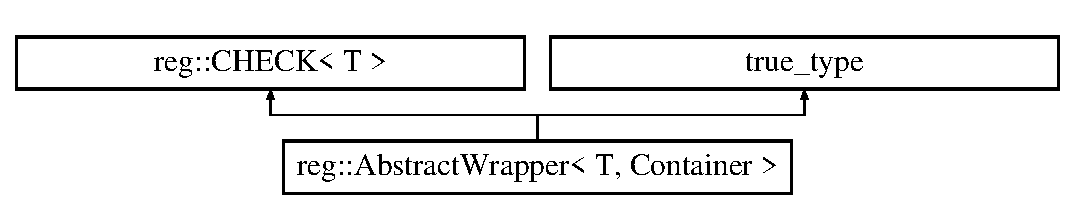
\includegraphics[height=2.000000cm]{structreg_1_1_abstract_wrapper}
\end{center}
\end{figure}
\subsection*{Public Types}
\begin{DoxyCompactItemize}
\item 
using \hyperlink{structreg_1_1_abstract_wrapper_a65e2282260e636ac1956862c158caa59}{self\+\_\+type} = T
\begin{DoxyCompactList}\small\item\em for introspection \end{DoxyCompactList}\end{DoxyCompactItemize}
\subsection*{Protected Member Functions}
\begin{DoxyCompactItemize}
\item 
\hyperlink{structreg_1_1_abstract_wrapper_a1b932145981f0c3f71466707725d772f}{Abstract\+Wrapper} ()
\begin{DoxyCompactList}\small\item\em R\+T\+TI. \end{DoxyCompactList}\item 
virtual T $\ast$ \hyperlink{structreg_1_1_abstract_wrapper_a88e7079432573b09a5cd695be34e9147}{Get} () const noexcept=0
\item 
virtual void \hyperlink{structreg_1_1_abstract_wrapper_af017f2af039fd5b940345e930e4bb397}{Set} (T $\ast$) noexcept=0
\item 
virtual void \hyperlink{structreg_1_1_abstract_wrapper_aad461ca147a0a7fcfd4f8662994742f3}{Allocate} () noexcept=0
\end{DoxyCompactItemize}
\subsection*{Protected Attributes}
\begin{DoxyCompactItemize}
\item 
Container \hyperlink{structreg_1_1_abstract_wrapper_a76a3713665e76d5ef8437681c7f309aa}{container\+\_\+}
\end{DoxyCompactItemize}


\subsection{Detailed Description}
\subsubsection*{template$<$typename T, typename Container$>$\newline
struct reg\+::\+Abstract\+Wrapper$<$ T, Container $>$}

abstract class for all \hyperlink{structreg_1_1_wrapper}{Wrapper} classes 

$<$ check if \hyperlink{structreg_1_1_wrapper}{Wrapper} inherits any specialized \hyperlink{structreg_1_1_wrapper_base}{Wrapper\+Base} structs

encapsulates data 
\begin{DoxyParams}{Parameters}
{\em T} & contained type \\
\hline
{\em Container} & container type \\
\hline
\end{DoxyParams}
\begin{DoxyNote}{Note}
R\+T\+TI 
\end{DoxyNote}


Definition at line 21 of file Wrapper.\+h.



\subsection{Member Typedef Documentation}
\mbox{\Hypertarget{structreg_1_1_abstract_wrapper_a65e2282260e636ac1956862c158caa59}\label{structreg_1_1_abstract_wrapper_a65e2282260e636ac1956862c158caa59}} 
\index{reg\+::\+Abstract\+Wrapper@{reg\+::\+Abstract\+Wrapper}!self\+\_\+type@{self\+\_\+type}}
\index{self\+\_\+type@{self\+\_\+type}!reg\+::\+Abstract\+Wrapper@{reg\+::\+Abstract\+Wrapper}}
\subsubsection{\texorpdfstring{self\+\_\+type}{self\_type}}
{\footnotesize\ttfamily template$<$typename T, typename Container$>$ \\
using \hyperlink{structreg_1_1_abstract_wrapper}{reg\+::\+Abstract\+Wrapper}$<$ T, Container $>$\+::\hyperlink{structreg_1_1_abstract_wrapper_a65e2282260e636ac1956862c158caa59}{self\+\_\+type} =  T}



for introspection 



Definition at line 25 of file Wrapper.\+h.



\subsection{Constructor \& Destructor Documentation}
\mbox{\Hypertarget{structreg_1_1_abstract_wrapper_a1b932145981f0c3f71466707725d772f}\label{structreg_1_1_abstract_wrapper_a1b932145981f0c3f71466707725d772f}} 
\index{reg\+::\+Abstract\+Wrapper@{reg\+::\+Abstract\+Wrapper}!Abstract\+Wrapper@{Abstract\+Wrapper}}
\index{Abstract\+Wrapper@{Abstract\+Wrapper}!reg\+::\+Abstract\+Wrapper@{reg\+::\+Abstract\+Wrapper}}
\subsubsection{\texorpdfstring{Abstract\+Wrapper()}{AbstractWrapper()}}
{\footnotesize\ttfamily template$<$typename T, typename Container$>$ \\
\hyperlink{structreg_1_1_abstract_wrapper}{reg\+::\+Abstract\+Wrapper}$<$ T, Container $>$\+::\hyperlink{structreg_1_1_abstract_wrapper}{Abstract\+Wrapper} (\begin{DoxyParamCaption}{ }\end{DoxyParamCaption})\hspace{0.3cm}{\ttfamily [inline]}, {\ttfamily [protected]}}



R\+T\+TI. 



Definition at line 28 of file Wrapper.\+h.



\subsection{Member Function Documentation}
\mbox{\Hypertarget{structreg_1_1_abstract_wrapper_aad461ca147a0a7fcfd4f8662994742f3}\label{structreg_1_1_abstract_wrapper_aad461ca147a0a7fcfd4f8662994742f3}} 
\index{reg\+::\+Abstract\+Wrapper@{reg\+::\+Abstract\+Wrapper}!Allocate@{Allocate}}
\index{Allocate@{Allocate}!reg\+::\+Abstract\+Wrapper@{reg\+::\+Abstract\+Wrapper}}
\subsubsection{\texorpdfstring{Allocate()}{Allocate()}}
{\footnotesize\ttfamily template$<$typename T, typename Container$>$ \\
virtual void \hyperlink{structreg_1_1_abstract_wrapper}{reg\+::\+Abstract\+Wrapper}$<$ T, Container $>$\+::Allocate (\begin{DoxyParamCaption}{ }\end{DoxyParamCaption})\hspace{0.3cm}{\ttfamily [protected]}, {\ttfamily [pure virtual]}, {\ttfamily [noexcept]}}



Implemented in \hyperlink{structreg_1_1_wrapper_base_3_01_t_00_01vtk_smart_pointer_3_01_t_01_4_01_4_a3b2609bc1666d9f2dbfe789100889bdc}{reg\+::\+Wrapper\+Base$<$ T, vtk\+Smart\+Pointer$<$ T $>$ $>$}, \hyperlink{structreg_1_1_wrapper_base_3_01_t_00_01itk_1_1_smart_pointer_3_01_t_01_4_01_4_a10fb689e5da772970c04d312d600868d}{reg\+::\+Wrapper\+Base$<$ T, itk\+::\+Smart\+Pointer$<$ T $>$ $>$}, and \hyperlink{structreg_1_1_wrapper_base_3_01_t_00_01std_1_1unique__ptr_3_01_t_01_4_01_4_a1b7e67476da7973f319d68e65543d1be}{reg\+::\+Wrapper\+Base$<$ T, std\+::unique\+\_\+ptr$<$ T $>$ $>$}.

\mbox{\Hypertarget{structreg_1_1_abstract_wrapper_a88e7079432573b09a5cd695be34e9147}\label{structreg_1_1_abstract_wrapper_a88e7079432573b09a5cd695be34e9147}} 
\index{reg\+::\+Abstract\+Wrapper@{reg\+::\+Abstract\+Wrapper}!Get@{Get}}
\index{Get@{Get}!reg\+::\+Abstract\+Wrapper@{reg\+::\+Abstract\+Wrapper}}
\subsubsection{\texorpdfstring{Get()}{Get()}}
{\footnotesize\ttfamily template$<$typename T, typename Container$>$ \\
virtual T$\ast$ \hyperlink{structreg_1_1_abstract_wrapper}{reg\+::\+Abstract\+Wrapper}$<$ T, Container $>$\+::Get (\begin{DoxyParamCaption}{ }\end{DoxyParamCaption}) const\hspace{0.3cm}{\ttfamily [protected]}, {\ttfamily [pure virtual]}, {\ttfamily [noexcept]}}



Implemented in \hyperlink{structreg_1_1_wrapper_base_3_01_t_00_01vtk_smart_pointer_3_01_t_01_4_01_4_a61bd745924ef0582ee61ae174ed7479f}{reg\+::\+Wrapper\+Base$<$ T, vtk\+Smart\+Pointer$<$ T $>$ $>$}, \hyperlink{structreg_1_1_wrapper_base_3_01_t_00_01itk_1_1_smart_pointer_3_01_t_01_4_01_4_ac2d57c43556c87aa45dcafd2c8a9cb47}{reg\+::\+Wrapper\+Base$<$ T, itk\+::\+Smart\+Pointer$<$ T $>$ $>$}, and \hyperlink{structreg_1_1_wrapper_base_3_01_t_00_01std_1_1unique__ptr_3_01_t_01_4_01_4_a9f4701d60f0dee6b61ae4046633f3ebe}{reg\+::\+Wrapper\+Base$<$ T, std\+::unique\+\_\+ptr$<$ T $>$ $>$}.

\mbox{\Hypertarget{structreg_1_1_abstract_wrapper_af017f2af039fd5b940345e930e4bb397}\label{structreg_1_1_abstract_wrapper_af017f2af039fd5b940345e930e4bb397}} 
\index{reg\+::\+Abstract\+Wrapper@{reg\+::\+Abstract\+Wrapper}!Set@{Set}}
\index{Set@{Set}!reg\+::\+Abstract\+Wrapper@{reg\+::\+Abstract\+Wrapper}}
\subsubsection{\texorpdfstring{Set()}{Set()}}
{\footnotesize\ttfamily template$<$typename T, typename Container$>$ \\
virtual void \hyperlink{structreg_1_1_abstract_wrapper}{reg\+::\+Abstract\+Wrapper}$<$ T, Container $>$\+::Set (\begin{DoxyParamCaption}\item[{T $\ast$}]{ }\end{DoxyParamCaption})\hspace{0.3cm}{\ttfamily [protected]}, {\ttfamily [pure virtual]}, {\ttfamily [noexcept]}}



Implemented in \hyperlink{structreg_1_1_wrapper_base_3_01_t_00_01vtk_smart_pointer_3_01_t_01_4_01_4_aa066a74ca5abf0e13fd3ed62f0508e32}{reg\+::\+Wrapper\+Base$<$ T, vtk\+Smart\+Pointer$<$ T $>$ $>$}, \hyperlink{structreg_1_1_wrapper_base_3_01_t_00_01itk_1_1_smart_pointer_3_01_t_01_4_01_4_a9a9bcfbe7236f66cb355f929aeeca281}{reg\+::\+Wrapper\+Base$<$ T, itk\+::\+Smart\+Pointer$<$ T $>$ $>$}, and \hyperlink{structreg_1_1_wrapper_base_3_01_t_00_01std_1_1unique__ptr_3_01_t_01_4_01_4_a280dc1e6a85e2a95eaa849a45169942f}{reg\+::\+Wrapper\+Base$<$ T, std\+::unique\+\_\+ptr$<$ T $>$ $>$}.



\subsection{Member Data Documentation}
\mbox{\Hypertarget{structreg_1_1_abstract_wrapper_a76a3713665e76d5ef8437681c7f309aa}\label{structreg_1_1_abstract_wrapper_a76a3713665e76d5ef8437681c7f309aa}} 
\index{reg\+::\+Abstract\+Wrapper@{reg\+::\+Abstract\+Wrapper}!container\+\_\+@{container\+\_\+}}
\index{container\+\_\+@{container\+\_\+}!reg\+::\+Abstract\+Wrapper@{reg\+::\+Abstract\+Wrapper}}
\subsubsection{\texorpdfstring{container\+\_\+}{container\_}}
{\footnotesize\ttfamily template$<$typename T, typename Container$>$ \\
Container \hyperlink{structreg_1_1_abstract_wrapper}{reg\+::\+Abstract\+Wrapper}$<$ T, Container $>$\+::container\+\_\+\hspace{0.3cm}{\ttfamily [protected]}}



Definition at line 35 of file Wrapper.\+h.



The documentation for this struct was generated from the following file\+:\begin{DoxyCompactItemize}
\item 
/home/adam/\+Desktop/reg/\+Wrapper/\hyperlink{_wrapper_8h}{Wrapper.\+h}\end{DoxyCompactItemize}

\hypertarget{structreg_1_1_c_h_e_c_k}{}\section{reg\+:\+:C\+H\+E\+CK$<$ T $>$ Struct Template Reference}
\label{structreg_1_1_c_h_e_c_k}\index{reg\+::\+C\+H\+E\+C\+K$<$ T $>$@{reg\+::\+C\+H\+E\+C\+K$<$ T $>$}}


error checking class  




{\ttfamily \#include $<$C\+H\+E\+C\+K.\+h$>$}

Inheritance diagram for reg\+:\+:C\+H\+E\+CK$<$ T $>$\+:\begin{figure}[H]
\begin{center}
\leavevmode
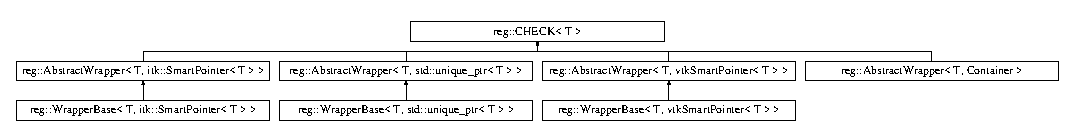
\includegraphics[height=1.390728cm]{structreg_1_1_c_h_e_c_k}
\end{center}
\end{figure}
\subsection*{Protected Member Functions}
\begin{DoxyCompactItemize}
\item 
void \hyperlink{structreg_1_1_c_h_e_c_k_a71d36138703b538aebcd1ca2dabd2d63}{N\+U\+L\+L\+P\+T\+R\+\_\+\+E\+R\+R\+OR} (T $\ast$t, std\+::string \&\&msg=\char`\"{}N\+U\+L\+L\+P\+T\+R\+\_\+\+E\+R\+R\+OR\char`\"{}) const noexcept
\item 
void \hyperlink{structreg_1_1_c_h_e_c_k_ab3559ddae75930312bb95e57dc07f655}{N\+U\+L\+L\+P\+T\+R\+\_\+\+N\+O\+TE} (T $\ast$t, std\+::string \&\&msg=\char`\"{}N\+U\+L\+L\+P\+T\+R\+\_\+\+N\+O\+TE\char`\"{}) const noexcept
\item 
void \hyperlink{structreg_1_1_c_h_e_c_k_aaa2449b02889f76964587061684795d2}{N\+U\+L\+L\+P\+T\+R\+\_\+\+W\+A\+R\+N\+I\+NG} (T $\ast$t, std\+::string \&\&msg=\char`\"{}N\+U\+L\+L\+P\+T\+R\+\_\+\+W\+A\+R\+N\+I\+NG\char`\"{}) const noexcept
\end{DoxyCompactItemize}


\subsection{Detailed Description}
\subsubsection*{template$<$typename T$>$\newline
struct reg\+::\+C\+H\+E\+C\+K$<$ T $>$}

error checking class 

avoid exceptions because they cause undefined behavior; rather, use detailed reporting \begin{DoxyNote}{Note}
every class should directly or indirectly be derived from this class 
\end{DoxyNote}

\begin{DoxyParams}{Parameters}
{\em T} & the base type to monitor \\
\hline
\end{DoxyParams}


Definition at line 15 of file C\+H\+E\+C\+K.\+h.



\subsection{Member Function Documentation}
\mbox{\Hypertarget{structreg_1_1_c_h_e_c_k_a71d36138703b538aebcd1ca2dabd2d63}\label{structreg_1_1_c_h_e_c_k_a71d36138703b538aebcd1ca2dabd2d63}} 
\index{reg\+::\+C\+H\+E\+CK@{reg\+::\+C\+H\+E\+CK}!N\+U\+L\+L\+P\+T\+R\+\_\+\+E\+R\+R\+OR@{N\+U\+L\+L\+P\+T\+R\+\_\+\+E\+R\+R\+OR}}
\index{N\+U\+L\+L\+P\+T\+R\+\_\+\+E\+R\+R\+OR@{N\+U\+L\+L\+P\+T\+R\+\_\+\+E\+R\+R\+OR}!reg\+::\+C\+H\+E\+CK@{reg\+::\+C\+H\+E\+CK}}
\subsubsection{\texorpdfstring{N\+U\+L\+L\+P\+T\+R\+\_\+\+E\+R\+R\+O\+R()}{NULLPTR\_ERROR()}}
{\footnotesize\ttfamily template$<$typename T$>$ \\
void \hyperlink{structreg_1_1_c_h_e_c_k}{reg\+::\+C\+H\+E\+CK}$<$ T $>$\+::N\+U\+L\+L\+P\+T\+R\+\_\+\+E\+R\+R\+OR (\begin{DoxyParamCaption}\item[{T $\ast$}]{t,  }\item[{std\+::string \&\&}]{msg = {\ttfamily \char`\"{}NULLPTR\+\_\+ERROR\char`\"{}} }\end{DoxyParamCaption}) const\hspace{0.3cm}{\ttfamily [inline]}, {\ttfamily [protected]}, {\ttfamily [noexcept]}}



Definition at line 17 of file C\+H\+E\+C\+K.\+h.

\mbox{\Hypertarget{structreg_1_1_c_h_e_c_k_ab3559ddae75930312bb95e57dc07f655}\label{structreg_1_1_c_h_e_c_k_ab3559ddae75930312bb95e57dc07f655}} 
\index{reg\+::\+C\+H\+E\+CK@{reg\+::\+C\+H\+E\+CK}!N\+U\+L\+L\+P\+T\+R\+\_\+\+N\+O\+TE@{N\+U\+L\+L\+P\+T\+R\+\_\+\+N\+O\+TE}}
\index{N\+U\+L\+L\+P\+T\+R\+\_\+\+N\+O\+TE@{N\+U\+L\+L\+P\+T\+R\+\_\+\+N\+O\+TE}!reg\+::\+C\+H\+E\+CK@{reg\+::\+C\+H\+E\+CK}}
\subsubsection{\texorpdfstring{N\+U\+L\+L\+P\+T\+R\+\_\+\+N\+O\+T\+E()}{NULLPTR\_NOTE()}}
{\footnotesize\ttfamily template$<$typename T$>$ \\
void \hyperlink{structreg_1_1_c_h_e_c_k}{reg\+::\+C\+H\+E\+CK}$<$ T $>$\+::N\+U\+L\+L\+P\+T\+R\+\_\+\+N\+O\+TE (\begin{DoxyParamCaption}\item[{T $\ast$}]{t,  }\item[{std\+::string \&\&}]{msg = {\ttfamily \char`\"{}NULLPTR\+\_\+NOTE\char`\"{}} }\end{DoxyParamCaption}) const\hspace{0.3cm}{\ttfamily [inline]}, {\ttfamily [protected]}, {\ttfamily [noexcept]}}



Definition at line 21 of file C\+H\+E\+C\+K.\+h.

\mbox{\Hypertarget{structreg_1_1_c_h_e_c_k_aaa2449b02889f76964587061684795d2}\label{structreg_1_1_c_h_e_c_k_aaa2449b02889f76964587061684795d2}} 
\index{reg\+::\+C\+H\+E\+CK@{reg\+::\+C\+H\+E\+CK}!N\+U\+L\+L\+P\+T\+R\+\_\+\+W\+A\+R\+N\+I\+NG@{N\+U\+L\+L\+P\+T\+R\+\_\+\+W\+A\+R\+N\+I\+NG}}
\index{N\+U\+L\+L\+P\+T\+R\+\_\+\+W\+A\+R\+N\+I\+NG@{N\+U\+L\+L\+P\+T\+R\+\_\+\+W\+A\+R\+N\+I\+NG}!reg\+::\+C\+H\+E\+CK@{reg\+::\+C\+H\+E\+CK}}
\subsubsection{\texorpdfstring{N\+U\+L\+L\+P\+T\+R\+\_\+\+W\+A\+R\+N\+I\+N\+G()}{NULLPTR\_WARNING()}}
{\footnotesize\ttfamily template$<$typename T$>$ \\
void \hyperlink{structreg_1_1_c_h_e_c_k}{reg\+::\+C\+H\+E\+CK}$<$ T $>$\+::N\+U\+L\+L\+P\+T\+R\+\_\+\+W\+A\+R\+N\+I\+NG (\begin{DoxyParamCaption}\item[{T $\ast$}]{t,  }\item[{std\+::string \&\&}]{msg = {\ttfamily \char`\"{}NULLPTR\+\_\+WARNING\char`\"{}} }\end{DoxyParamCaption}) const\hspace{0.3cm}{\ttfamily [inline]}, {\ttfamily [protected]}, {\ttfamily [noexcept]}}



Definition at line 25 of file C\+H\+E\+C\+K.\+h.



The documentation for this struct was generated from the following file\+:\begin{DoxyCompactItemize}
\item 
/home/adam/\+Desktop/reg/\+C\+H\+E\+C\+K/\hyperlink{_c_h_e_c_k_8h}{C\+H\+E\+C\+K.\+h}\end{DoxyCompactItemize}

\hypertarget{structreg_1_1_combined}{}\section{reg\+:\+:Combined Struct Reference}
\label{structreg_1_1_combined}\index{reg\+::\+Combined@{reg\+::\+Combined}}


{\ttfamily \#include $<$Registrator.\+h$>$}

Inheritance diagram for reg\+:\+:Combined\+:\begin{figure}[H]
\begin{center}
\leavevmode
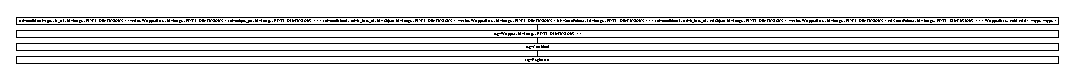
\includegraphics[height=0.625698cm]{structreg_1_1_combined}
\end{center}
\end{figure}


\subsection{Detailed Description}


Definition at line 18 of file Registrator.\+h.



The documentation for this struct was generated from the following file\+:\begin{DoxyCompactItemize}
\item 
/home/adam/\+Desktop/reg/\+Registrator/\hyperlink{_registrator_8h}{Registrator.\+h}\end{DoxyCompactItemize}

\hypertarget{class_command_iteration_update}{}\section{Command\+Iteration\+Update Class Reference}
\label{class_command_iteration_update}\index{Command\+Iteration\+Update@{Command\+Iteration\+Update}}


{\ttfamily \#include $<$Observer.\+h$>$}

Inheritance diagram for Command\+Iteration\+Update\+:\begin{figure}[H]
\begin{center}
\leavevmode
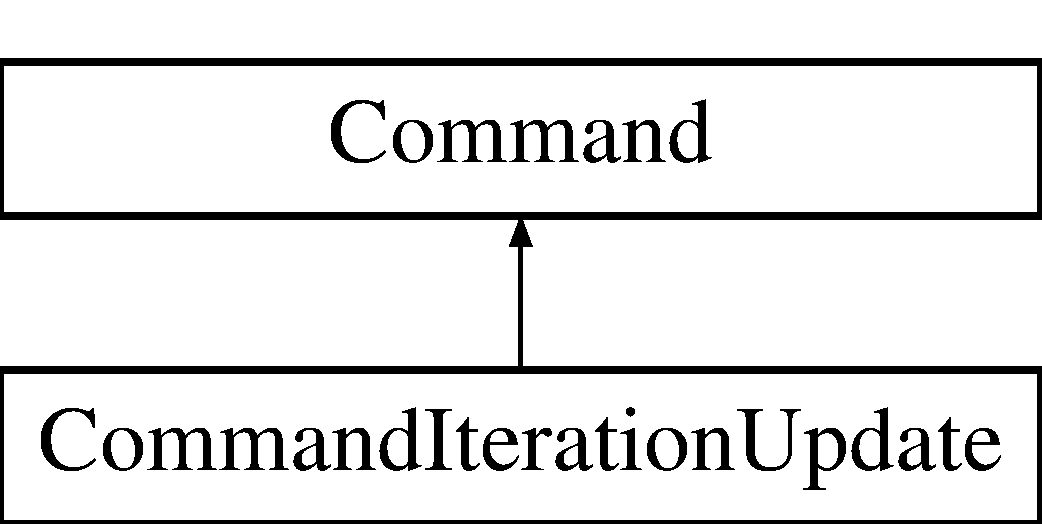
\includegraphics[height=2.000000cm]{class_command_iteration_update}
\end{center}
\end{figure}
\subsection*{Public Types}
\begin{DoxyCompactItemize}
\item 
typedef \hyperlink{class_command_iteration_update}{Command\+Iteration\+Update} \hyperlink{class_command_iteration_update_a82da0970ef8c14141f85f3465f08242e}{Self}
\item 
typedef itk\+::\+Command \hyperlink{class_command_iteration_update_a7321e36a5179cac3cf6dc00de2d5f494}{Superclass}
\item 
typedef itk\+::\+Smart\+Pointer$<$ \hyperlink{class_command_iteration_update_a82da0970ef8c14141f85f3465f08242e}{Self} $>$ \hyperlink{class_command_iteration_update_a07d09836044e93fd8693d947d77a58a5}{Pointer}
\item 
typedef itk\+::\+Gradient\+Descent\+Optimizerv4\+Template$<$ double $>$ \hyperlink{class_command_iteration_update_aa3ff4b0f0b936c866d1bed92cacaf6a1}{Optimizer\+Type}
\item 
typedef const \hyperlink{class_command_iteration_update_aa3ff4b0f0b936c866d1bed92cacaf6a1}{Optimizer\+Type} $\ast$ \hyperlink{class_command_iteration_update_aed2829c5e03b1f7b5e9c862f00f493af}{Optimizer\+Pointer}
\end{DoxyCompactItemize}
\subsection*{Public Member Functions}
\begin{DoxyCompactItemize}
\item 
\hyperlink{class_command_iteration_update_a45a63d6e43a42eabd6adb27b1309c7a1}{itk\+New\+Macro} (\hyperlink{class_command_iteration_update_a82da0970ef8c14141f85f3465f08242e}{Self})
\item 
void \hyperlink{class_command_iteration_update_a9283ff36a470e597ea27e73a557d7c5f}{Execute} (itk\+::\+Object $\ast$caller, const itk\+::\+Event\+Object \&event) I\+T\+K\+\_\+\+O\+V\+E\+R\+R\+I\+DE
\item 
void \hyperlink{class_command_iteration_update_acb3a3b59afa764cf1b6d73190c33e6cb}{Execute} (const itk\+::\+Object $\ast$object, const itk\+::\+Event\+Object \&event) I\+T\+K\+\_\+\+O\+V\+E\+R\+R\+I\+DE
\end{DoxyCompactItemize}
\subsection*{Protected Member Functions}
\begin{DoxyCompactItemize}
\item 
\hyperlink{class_command_iteration_update_a3b6dc4b6e947779a656ce69152377a70}{Command\+Iteration\+Update} ()
\end{DoxyCompactItemize}


\subsection{Detailed Description}
\begin{DoxySeeAlso}{See also}
\href{https://itk.org/Doxygen45/html/Registration_2ImageRegistration8_8cxx-example.html}{\tt https\+://itk.\+org/\+Doxygen45/html/\+Registration\+\_\+2\+Image\+Registration8\+\_\+8cxx-\/example.\+html} 
\end{DoxySeeAlso}
\begin{DoxyNote}{Note}
uses itk\+::\+Gradient\+Descent\+Optimizerv4\+Template$<$double$>$ instead 
\end{DoxyNote}
\begin{DoxyWarning}{Warning}
no considerations for extensibility 
\end{DoxyWarning}


Definition at line 20 of file Observer.\+h.



\subsection{Member Typedef Documentation}
\mbox{\Hypertarget{class_command_iteration_update_aed2829c5e03b1f7b5e9c862f00f493af}\label{class_command_iteration_update_aed2829c5e03b1f7b5e9c862f00f493af}} 
\index{Command\+Iteration\+Update@{Command\+Iteration\+Update}!Optimizer\+Pointer@{Optimizer\+Pointer}}
\index{Optimizer\+Pointer@{Optimizer\+Pointer}!Command\+Iteration\+Update@{Command\+Iteration\+Update}}
\subsubsection{\texorpdfstring{Optimizer\+Pointer}{OptimizerPointer}}
{\footnotesize\ttfamily typedef const \hyperlink{class_command_iteration_update_aa3ff4b0f0b936c866d1bed92cacaf6a1}{Optimizer\+Type}$\ast$ \hyperlink{class_command_iteration_update_aed2829c5e03b1f7b5e9c862f00f493af}{Command\+Iteration\+Update\+::\+Optimizer\+Pointer}}



Definition at line 32 of file Observer.\+h.

\mbox{\Hypertarget{class_command_iteration_update_aa3ff4b0f0b936c866d1bed92cacaf6a1}\label{class_command_iteration_update_aa3ff4b0f0b936c866d1bed92cacaf6a1}} 
\index{Command\+Iteration\+Update@{Command\+Iteration\+Update}!Optimizer\+Type@{Optimizer\+Type}}
\index{Optimizer\+Type@{Optimizer\+Type}!Command\+Iteration\+Update@{Command\+Iteration\+Update}}
\subsubsection{\texorpdfstring{Optimizer\+Type}{OptimizerType}}
{\footnotesize\ttfamily typedef itk\+::\+Gradient\+Descent\+Optimizerv4\+Template$<$double$>$ \hyperlink{class_command_iteration_update_aa3ff4b0f0b936c866d1bed92cacaf6a1}{Command\+Iteration\+Update\+::\+Optimizer\+Type}}



Definition at line 28 of file Observer.\+h.

\mbox{\Hypertarget{class_command_iteration_update_a07d09836044e93fd8693d947d77a58a5}\label{class_command_iteration_update_a07d09836044e93fd8693d947d77a58a5}} 
\index{Command\+Iteration\+Update@{Command\+Iteration\+Update}!Pointer@{Pointer}}
\index{Pointer@{Pointer}!Command\+Iteration\+Update@{Command\+Iteration\+Update}}
\subsubsection{\texorpdfstring{Pointer}{Pointer}}
{\footnotesize\ttfamily typedef itk\+::\+Smart\+Pointer$<$\hyperlink{class_command_iteration_update_a82da0970ef8c14141f85f3465f08242e}{Self}$>$ \hyperlink{class_command_iteration_update_a07d09836044e93fd8693d947d77a58a5}{Command\+Iteration\+Update\+::\+Pointer}}



Definition at line 24 of file Observer.\+h.

\mbox{\Hypertarget{class_command_iteration_update_a82da0970ef8c14141f85f3465f08242e}\label{class_command_iteration_update_a82da0970ef8c14141f85f3465f08242e}} 
\index{Command\+Iteration\+Update@{Command\+Iteration\+Update}!Self@{Self}}
\index{Self@{Self}!Command\+Iteration\+Update@{Command\+Iteration\+Update}}
\subsubsection{\texorpdfstring{Self}{Self}}
{\footnotesize\ttfamily typedef \hyperlink{class_command_iteration_update}{Command\+Iteration\+Update} \hyperlink{class_command_iteration_update_a82da0970ef8c14141f85f3465f08242e}{Command\+Iteration\+Update\+::\+Self}}



Definition at line 22 of file Observer.\+h.

\mbox{\Hypertarget{class_command_iteration_update_a7321e36a5179cac3cf6dc00de2d5f494}\label{class_command_iteration_update_a7321e36a5179cac3cf6dc00de2d5f494}} 
\index{Command\+Iteration\+Update@{Command\+Iteration\+Update}!Superclass@{Superclass}}
\index{Superclass@{Superclass}!Command\+Iteration\+Update@{Command\+Iteration\+Update}}
\subsubsection{\texorpdfstring{Superclass}{Superclass}}
{\footnotesize\ttfamily typedef itk\+::\+Command \hyperlink{class_command_iteration_update_a7321e36a5179cac3cf6dc00de2d5f494}{Command\+Iteration\+Update\+::\+Superclass}}



Definition at line 23 of file Observer.\+h.



\subsection{Constructor \& Destructor Documentation}
\mbox{\Hypertarget{class_command_iteration_update_a3b6dc4b6e947779a656ce69152377a70}\label{class_command_iteration_update_a3b6dc4b6e947779a656ce69152377a70}} 
\index{Command\+Iteration\+Update@{Command\+Iteration\+Update}!Command\+Iteration\+Update@{Command\+Iteration\+Update}}
\index{Command\+Iteration\+Update@{Command\+Iteration\+Update}!Command\+Iteration\+Update@{Command\+Iteration\+Update}}
\subsubsection{\texorpdfstring{Command\+Iteration\+Update()}{CommandIterationUpdate()}}
{\footnotesize\ttfamily Command\+Iteration\+Update\+::\+Command\+Iteration\+Update (\begin{DoxyParamCaption}{ }\end{DoxyParamCaption})\hspace{0.3cm}{\ttfamily [inline]}, {\ttfamily [protected]}}



Definition at line 28 of file Observer.\+h.



\subsection{Member Function Documentation}
\mbox{\Hypertarget{class_command_iteration_update_a9283ff36a470e597ea27e73a557d7c5f}\label{class_command_iteration_update_a9283ff36a470e597ea27e73a557d7c5f}} 
\index{Command\+Iteration\+Update@{Command\+Iteration\+Update}!Execute@{Execute}}
\index{Execute@{Execute}!Command\+Iteration\+Update@{Command\+Iteration\+Update}}
\subsubsection{\texorpdfstring{Execute()}{Execute()}\hspace{0.1cm}{\footnotesize\ttfamily [1/2]}}
{\footnotesize\ttfamily void Command\+Iteration\+Update\+::\+Execute (\begin{DoxyParamCaption}\item[{itk\+::\+Object $\ast$}]{caller,  }\item[{const itk\+::\+Event\+Object \&}]{event }\end{DoxyParamCaption})\hspace{0.3cm}{\ttfamily [inline]}}



Definition at line 33 of file Observer.\+h.

\mbox{\Hypertarget{class_command_iteration_update_acb3a3b59afa764cf1b6d73190c33e6cb}\label{class_command_iteration_update_acb3a3b59afa764cf1b6d73190c33e6cb}} 
\index{Command\+Iteration\+Update@{Command\+Iteration\+Update}!Execute@{Execute}}
\index{Execute@{Execute}!Command\+Iteration\+Update@{Command\+Iteration\+Update}}
\subsubsection{\texorpdfstring{Execute()}{Execute()}\hspace{0.1cm}{\footnotesize\ttfamily [2/2]}}
{\footnotesize\ttfamily void Command\+Iteration\+Update\+::\+Execute (\begin{DoxyParamCaption}\item[{const itk\+::\+Object $\ast$}]{object,  }\item[{const itk\+::\+Event\+Object \&}]{event }\end{DoxyParamCaption})\hspace{0.3cm}{\ttfamily [inline]}}



Definition at line 37 of file Observer.\+h.

\mbox{\Hypertarget{class_command_iteration_update_a45a63d6e43a42eabd6adb27b1309c7a1}\label{class_command_iteration_update_a45a63d6e43a42eabd6adb27b1309c7a1}} 
\index{Command\+Iteration\+Update@{Command\+Iteration\+Update}!itk\+New\+Macro@{itk\+New\+Macro}}
\index{itk\+New\+Macro@{itk\+New\+Macro}!Command\+Iteration\+Update@{Command\+Iteration\+Update}}
\subsubsection{\texorpdfstring{itk\+New\+Macro()}{itkNewMacro()}}
{\footnotesize\ttfamily Command\+Iteration\+Update\+::itk\+New\+Macro (\begin{DoxyParamCaption}\item[{\hyperlink{class_command_iteration_update_a82da0970ef8c14141f85f3465f08242e}{Self}}]{ }\end{DoxyParamCaption})}



The documentation for this class was generated from the following file\+:\begin{DoxyCompactItemize}
\item 
/home/adam/\+Desktop/reg/\+Observer/\hyperlink{_observer_8h}{Observer.\+h}\end{DoxyCompactItemize}

\hypertarget{structreg_1_1_composite_opacity}{}\section{reg\+:\+:Composite\+Opacity Struct Reference}
\label{structreg_1_1_composite_opacity}\index{reg\+::\+Composite\+Opacity@{reg\+::\+Composite\+Opacity}}


alias for \hyperlink{structreg_1_1_wrapper}{Wrapper$<$vtk\+Piecewise\+Function$>$} for disambiguation  




{\ttfamily \#include $<$Visualizer.\+h$>$}

Inheritance diagram for reg\+:\+:Composite\+Opacity\+:\begin{figure}[H]
\begin{center}
\leavevmode
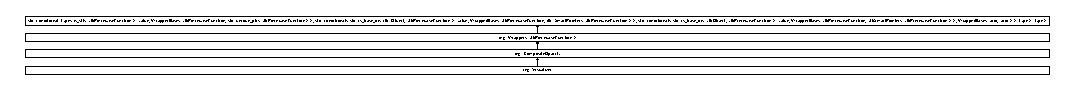
\includegraphics[height=0.771084cm]{structreg_1_1_composite_opacity}
\end{center}
\end{figure}


\subsection{Detailed Description}
alias for \hyperlink{structreg_1_1_wrapper}{Wrapper$<$vtk\+Piecewise\+Function$>$} for disambiguation 

Definition at line 18 of file Visualizer.\+h.



The documentation for this struct was generated from the following file\+:\begin{DoxyCompactItemize}
\item 
/home/adam/\+Desktop/reg/\+Visualizer/\hyperlink{_visualizer_8h}{Visualizer.\+h}\end{DoxyCompactItemize}

\hypertarget{structreg_1_1_fixed}{}\section{reg\+:\+:Fixed Struct Reference}
\label{structreg_1_1_fixed}\index{reg\+::\+Fixed@{reg\+::\+Fixed}}


{\ttfamily \#include $<$Registrator.\+h$>$}

Inheritance diagram for reg\+:\+:Fixed\+:\begin{figure}[H]
\begin{center}
\leavevmode
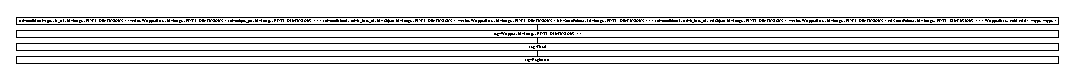
\includegraphics[height=0.625698cm]{structreg_1_1_fixed}
\end{center}
\end{figure}


\subsection{Detailed Description}


Definition at line 20 of file Registrator.\+h.



The documentation for this struct was generated from the following file\+:\begin{DoxyCompactItemize}
\item 
/home/adam/\+Desktop/reg/\+Registrator/\hyperlink{_registrator_8h}{Registrator.\+h}\end{DoxyCompactItemize}

\hypertarget{classitk_1_1_image_i_o_factory_register_manager}{}\section{itk\+:\+:Image\+I\+O\+Factory\+Register\+Manager Class Reference}
\label{classitk_1_1_image_i_o_factory_register_manager}\index{itk\+::\+Image\+I\+O\+Factory\+Register\+Manager@{itk\+::\+Image\+I\+O\+Factory\+Register\+Manager}}


{\ttfamily \#include $<$itk\+Image\+I\+O\+Factory\+Register\+Manager.\+h$>$}

\subsection*{Public Member Functions}
\begin{DoxyCompactItemize}
\item 
\hyperlink{classitk_1_1_image_i_o_factory_register_manager_aed949d5467196438d79b90abfcfb189b}{Image\+I\+O\+Factory\+Register\+Manager} (void($\ast$list\mbox{[}$\,$\mbox{]})(void))
\item 
\hyperlink{classitk_1_1_image_i_o_factory_register_manager_aed949d5467196438d79b90abfcfb189b}{Image\+I\+O\+Factory\+Register\+Manager} (void($\ast$list\mbox{[}$\,$\mbox{]})(void))
\end{DoxyCompactItemize}


\subsection{Detailed Description}


Definition at line 24 of file itk\+Image\+I\+O\+Factory\+Register\+Manager.\+h.



\subsection{Constructor \& Destructor Documentation}
\mbox{\Hypertarget{classitk_1_1_image_i_o_factory_register_manager_aed949d5467196438d79b90abfcfb189b}\label{classitk_1_1_image_i_o_factory_register_manager_aed949d5467196438d79b90abfcfb189b}} 
\index{itk\+::\+Image\+I\+O\+Factory\+Register\+Manager@{itk\+::\+Image\+I\+O\+Factory\+Register\+Manager}!Image\+I\+O\+Factory\+Register\+Manager@{Image\+I\+O\+Factory\+Register\+Manager}}
\index{Image\+I\+O\+Factory\+Register\+Manager@{Image\+I\+O\+Factory\+Register\+Manager}!itk\+::\+Image\+I\+O\+Factory\+Register\+Manager@{itk\+::\+Image\+I\+O\+Factory\+Register\+Manager}}
\subsubsection{\texorpdfstring{Image\+I\+O\+Factory\+Register\+Manager()}{ImageIOFactoryRegisterManager()}\hspace{0.1cm}{\footnotesize\ttfamily [1/2]}}
{\footnotesize\ttfamily itk\+::\+Image\+I\+O\+Factory\+Register\+Manager\+::\+Image\+I\+O\+Factory\+Register\+Manager (\begin{DoxyParamCaption}\item[{void($\ast$\mbox{[}$\,$\mbox{]})(void)}]{list }\end{DoxyParamCaption})\hspace{0.3cm}{\ttfamily [inline]}}



Definition at line 27 of file itk\+Image\+I\+O\+Factory\+Register\+Manager.\+h.

\mbox{\Hypertarget{classitk_1_1_image_i_o_factory_register_manager_aed949d5467196438d79b90abfcfb189b}\label{classitk_1_1_image_i_o_factory_register_manager_aed949d5467196438d79b90abfcfb189b}} 
\index{itk\+::\+Image\+I\+O\+Factory\+Register\+Manager@{itk\+::\+Image\+I\+O\+Factory\+Register\+Manager}!Image\+I\+O\+Factory\+Register\+Manager@{Image\+I\+O\+Factory\+Register\+Manager}}
\index{Image\+I\+O\+Factory\+Register\+Manager@{Image\+I\+O\+Factory\+Register\+Manager}!itk\+::\+Image\+I\+O\+Factory\+Register\+Manager@{itk\+::\+Image\+I\+O\+Factory\+Register\+Manager}}
\subsubsection{\texorpdfstring{Image\+I\+O\+Factory\+Register\+Manager()}{ImageIOFactoryRegisterManager()}\hspace{0.1cm}{\footnotesize\ttfamily [2/2]}}
{\footnotesize\ttfamily itk\+::\+Image\+I\+O\+Factory\+Register\+Manager\+::\+Image\+I\+O\+Factory\+Register\+Manager (\begin{DoxyParamCaption}\item[{void($\ast$\mbox{[}$\,$\mbox{]})(void)}]{list }\end{DoxyParamCaption})\hspace{0.3cm}{\ttfamily [inline]}}



Definition at line 27 of file itk\+Image\+I\+O\+Factory\+Register\+Manager.\+h.



The documentation for this class was generated from the following file\+:\begin{DoxyCompactItemize}
\item 
/home/adam/\+Desktop/reg/build/\+I\+T\+K\+I\+O\+Factory\+Registration/\hyperlink{build_2_i_t_k_i_o_factory_registration_2itk_image_i_o_factory_register_manager_8h}{itk\+Image\+I\+O\+Factory\+Register\+Manager.\+h}\end{DoxyCompactItemize}

\hypertarget{structreg_1_1_interpolator}{}\section{reg\+:\+:Interpolator Struct Reference}
\label{structreg_1_1_interpolator}\index{reg\+::\+Interpolator@{reg\+::\+Interpolator}}


{\ttfamily \#include $<$Registrator.\+h$>$}

Inheritance diagram for reg\+:\+:Interpolator\+:\begin{figure}[H]
\begin{center}
\leavevmode
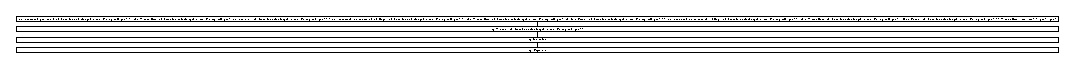
\includegraphics[height=0.479760cm]{structreg_1_1_interpolator}
\end{center}
\end{figure}


\subsection{Detailed Description}


Definition at line 30 of file Registrator.\+h.



The documentation for this struct was generated from the following file\+:\begin{DoxyCompactItemize}
\item 
/home/adam/\+Desktop/reg/\+Registrator/\hyperlink{_registrator_8h}{Registrator.\+h}\end{DoxyCompactItemize}

\hypertarget{structreg_1_1is__stl}{}\section{reg\+:\+:is\+\_\+stl$<$ typename $>$ Struct Template Reference}
\label{structreg_1_1is__stl}\index{reg\+::is\+\_\+stl$<$ typename $>$@{reg\+::is\+\_\+stl$<$ typename $>$}}


general template of \hyperlink{structreg_1_1is__stl}{is\+\_\+stl}  




{\ttfamily \#include $<$Wrapper.\+h$>$}

Inheritance diagram for reg\+:\+:is\+\_\+stl$<$ typename $>$\+:\begin{figure}[H]
\begin{center}
\leavevmode
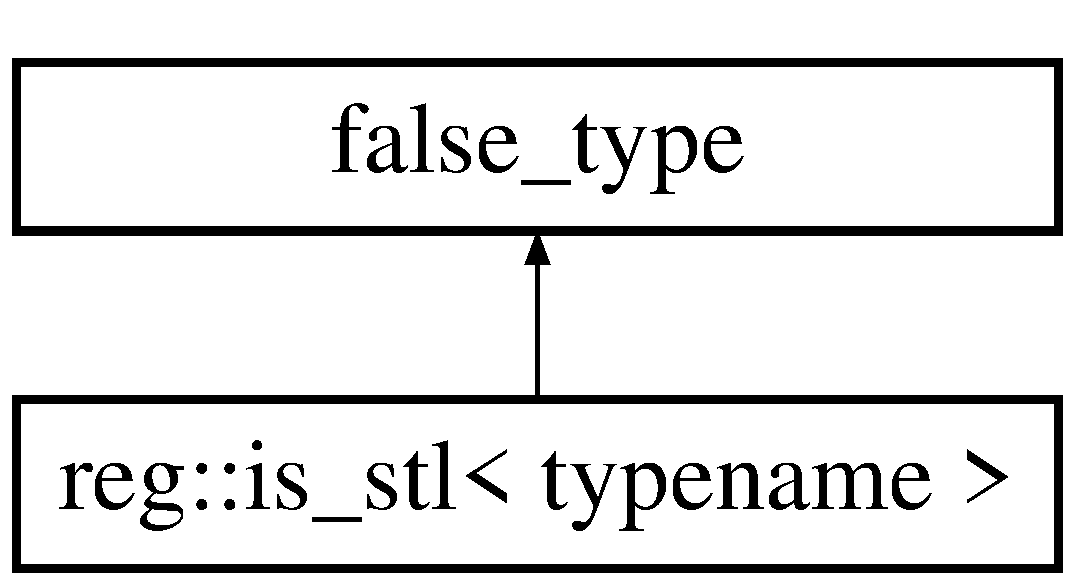
\includegraphics[height=2.000000cm]{structreg_1_1is__stl}
\end{center}
\end{figure}


\subsection{Detailed Description}
\subsubsection*{template$<$typename$>$\newline
struct reg\+::is\+\_\+stl$<$ typename $>$}

general template of \hyperlink{structreg_1_1is__stl}{is\+\_\+stl} 

specialized template of \hyperlink{structreg_1_1is__stl}{is\+\_\+stl}

check if type is S\+TL

detects any containers based on std\+::vector 
\begin{DoxyParams}{Parameters}
{\em T} & contained type \\
\hline
{\em Alloc} & S\+TL specific allocator\\
\hline
\end{DoxyParams}
detects std\+::string 

Definition at line 92 of file Wrapper.\+h.



The documentation for this struct was generated from the following file\+:\begin{DoxyCompactItemize}
\item 
/home/adam/\+Desktop/reg/\+Wrapper/\hyperlink{_wrapper_8h}{Wrapper.\+h}\end{DoxyCompactItemize}

\hypertarget{structreg_1_1is__stl_3_01std_1_1string_01_4}{}\section{reg\+:\+:is\+\_\+stl$<$ std\+:\+:string $>$ Struct Template Reference}
\label{structreg_1_1is__stl_3_01std_1_1string_01_4}\index{reg\+::is\+\_\+stl$<$ std\+::string $>$@{reg\+::is\+\_\+stl$<$ std\+::string $>$}}


{\ttfamily \#include $<$Wrapper.\+h$>$}

Inheritance diagram for reg\+:\+:is\+\_\+stl$<$ std\+:\+:string $>$\+:\begin{figure}[H]
\begin{center}
\leavevmode
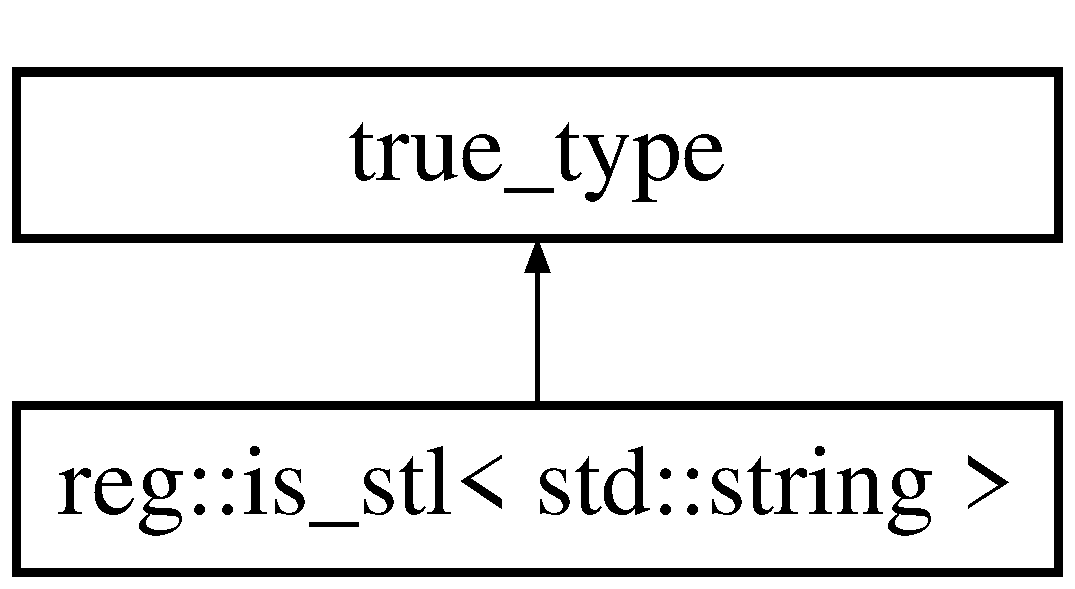
\includegraphics[height=2.000000cm]{structreg_1_1is__stl_3_01std_1_1string_01_4}
\end{center}
\end{figure}


\subsection{Detailed Description}
\subsubsection*{template$<$$>$\newline
struct reg\+::is\+\_\+stl$<$ std\+::string $>$}



Definition at line 105 of file Wrapper.\+h.



The documentation for this struct was generated from the following file\+:\begin{DoxyCompactItemize}
\item 
/home/adam/\+Desktop/reg/\+Wrapper/\hyperlink{_wrapper_8h}{Wrapper.\+h}\end{DoxyCompactItemize}

\hypertarget{structreg_1_1is__stl_3_01std_1_1vector_3_01_t_00_01_alloc_01_4_01_4}{}\section{reg\+:\+:is\+\_\+stl$<$ std\+:\+:vector$<$ T, Alloc $>$ $>$ Struct Template Reference}
\label{structreg_1_1is__stl_3_01std_1_1vector_3_01_t_00_01_alloc_01_4_01_4}\index{reg\+::is\+\_\+stl$<$ std\+::vector$<$ T, Alloc $>$ $>$@{reg\+::is\+\_\+stl$<$ std\+::vector$<$ T, Alloc $>$ $>$}}


{\ttfamily \#include $<$Wrapper.\+h$>$}

Inheritance diagram for reg\+:\+:is\+\_\+stl$<$ std\+:\+:vector$<$ T, Alloc $>$ $>$\+:\begin{figure}[H]
\begin{center}
\leavevmode
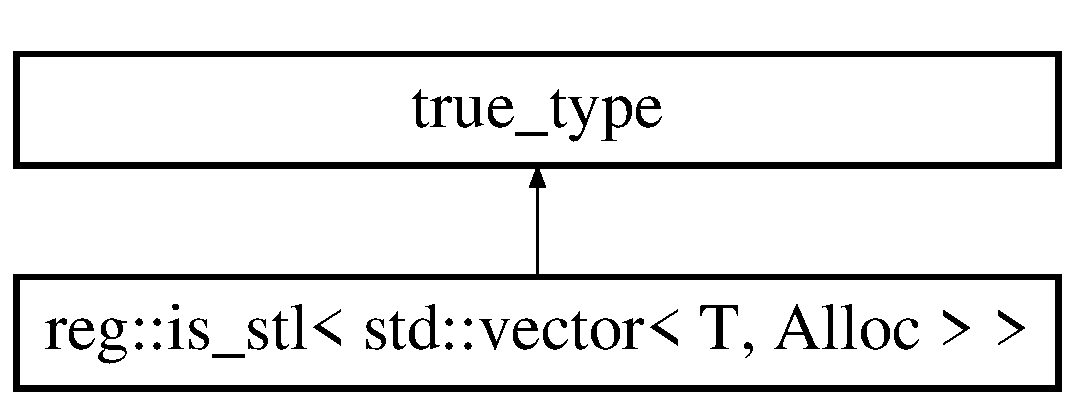
\includegraphics[height=2.000000cm]{structreg_1_1is__stl_3_01std_1_1vector_3_01_t_00_01_alloc_01_4_01_4}
\end{center}
\end{figure}


\subsection{Detailed Description}
\subsubsection*{template$<$typename T, typename Alloc$>$\newline
struct reg\+::is\+\_\+stl$<$ std\+::vector$<$ T, Alloc $>$ $>$}



Definition at line 100 of file Wrapper.\+h.



The documentation for this struct was generated from the following file\+:\begin{DoxyCompactItemize}
\item 
/home/adam/\+Desktop/reg/\+Wrapper/\hyperlink{_wrapper_8h}{Wrapper.\+h}\end{DoxyCompactItemize}

\hypertarget{structreg_1_1_i_t_kto_v_t_k}{}\section{reg\+:\+:I\+T\+Kto\+V\+TK Struct Reference}
\label{structreg_1_1_i_t_kto_v_t_k}\index{reg\+::\+I\+T\+Kto\+V\+TK@{reg\+::\+I\+T\+Kto\+V\+TK}}


converts itk\+::\+Image$<$double, 3$>$ to vtk\+::\+Image\+Data  




{\ttfamily \#include $<$I\+T\+Kto\+V\+T\+K.\+h$>$}

Inheritance diagram for reg\+:\+:I\+T\+Kto\+V\+TK\+:\begin{figure}[H]
\begin{center}
\leavevmode
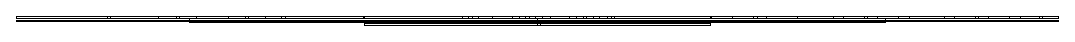
\includegraphics[height=0.123267cm]{structreg_1_1_i_t_kto_v_t_k}
\end{center}
\end{figure}
\subsection*{Public Member Functions}
\begin{DoxyCompactItemize}
\item 
\hyperlink{structreg_1_1_i_t_kto_v_t_k_aa877c393c7f899273ac90560680cccaa}{I\+T\+Kto\+V\+TK} ()=default
\item 
\hyperlink{structreg_1_1_i_t_kto_v_t_k_ae2fc7374133514e565fdb3e5d5dfad35}{I\+T\+Kto\+V\+TK} (itk\+::\+Image$<$ double, 3 $>$ $\ast$)
\item 
void \hyperlink{structreg_1_1_i_t_kto_v_t_k_a25b4c1792d1517d235f5c6d7319006f6}{Execute} (itk\+::\+Image$<$ double, 3 $>$ $\ast$)
\item 
void \hyperlink{structreg_1_1_i_t_kto_v_t_k_ab3e02f695618ce6ca0bb577b1cc97e7b}{Initialize} (itk\+::\+Image$<$ double, 3 $>$ $\ast$)
\end{DoxyCompactItemize}


\subsection{Detailed Description}
converts itk\+::\+Image$<$double, 3$>$ to vtk\+::\+Image\+Data 

\begin{DoxyWarning}{Warning}
requires itk to be built with I\+T\+K\+V\+T\+Kglue 
\end{DoxyWarning}


Definition at line 12 of file I\+T\+Kto\+V\+T\+K.\+h.



\subsection{Constructor \& Destructor Documentation}
\mbox{\Hypertarget{structreg_1_1_i_t_kto_v_t_k_aa877c393c7f899273ac90560680cccaa}\label{structreg_1_1_i_t_kto_v_t_k_aa877c393c7f899273ac90560680cccaa}} 
\index{reg\+::\+I\+T\+Kto\+V\+TK@{reg\+::\+I\+T\+Kto\+V\+TK}!I\+T\+Kto\+V\+TK@{I\+T\+Kto\+V\+TK}}
\index{I\+T\+Kto\+V\+TK@{I\+T\+Kto\+V\+TK}!reg\+::\+I\+T\+Kto\+V\+TK@{reg\+::\+I\+T\+Kto\+V\+TK}}
\subsubsection{\texorpdfstring{I\+T\+Kto\+V\+T\+K()}{ITKtoVTK()}\hspace{0.1cm}{\footnotesize\ttfamily [1/2]}}
{\footnotesize\ttfamily reg\+::\+I\+T\+Kto\+V\+T\+K\+::\+I\+T\+Kto\+V\+TK (\begin{DoxyParamCaption}{ }\end{DoxyParamCaption})\hspace{0.3cm}{\ttfamily [default]}}

\mbox{\Hypertarget{structreg_1_1_i_t_kto_v_t_k_ae2fc7374133514e565fdb3e5d5dfad35}\label{structreg_1_1_i_t_kto_v_t_k_ae2fc7374133514e565fdb3e5d5dfad35}} 
\index{reg\+::\+I\+T\+Kto\+V\+TK@{reg\+::\+I\+T\+Kto\+V\+TK}!I\+T\+Kto\+V\+TK@{I\+T\+Kto\+V\+TK}}
\index{I\+T\+Kto\+V\+TK@{I\+T\+Kto\+V\+TK}!reg\+::\+I\+T\+Kto\+V\+TK@{reg\+::\+I\+T\+Kto\+V\+TK}}
\subsubsection{\texorpdfstring{I\+T\+Kto\+V\+T\+K()}{ITKtoVTK()}\hspace{0.1cm}{\footnotesize\ttfamily [2/2]}}
{\footnotesize\ttfamily reg\+::\+I\+T\+Kto\+V\+T\+K\+::\+I\+T\+Kto\+V\+TK (\begin{DoxyParamCaption}\item[{itk\+::\+Image$<$ double, 3 $>$ $\ast$}]{itk\+\_\+image }\end{DoxyParamCaption})}



Definition at line 3 of file I\+T\+Kto\+V\+T\+K.\+cpp.



\subsection{Member Function Documentation}
\mbox{\Hypertarget{structreg_1_1_i_t_kto_v_t_k_a25b4c1792d1517d235f5c6d7319006f6}\label{structreg_1_1_i_t_kto_v_t_k_a25b4c1792d1517d235f5c6d7319006f6}} 
\index{reg\+::\+I\+T\+Kto\+V\+TK@{reg\+::\+I\+T\+Kto\+V\+TK}!Execute@{Execute}}
\index{Execute@{Execute}!reg\+::\+I\+T\+Kto\+V\+TK@{reg\+::\+I\+T\+Kto\+V\+TK}}
\subsubsection{\texorpdfstring{Execute()}{Execute()}}
{\footnotesize\ttfamily void reg\+::\+I\+T\+Kto\+V\+T\+K\+::\+Execute (\begin{DoxyParamCaption}\item[{itk\+::\+Image$<$ double, 3 $>$ $\ast$}]{itk\+\_\+image }\end{DoxyParamCaption})}



Definition at line 8 of file I\+T\+Kto\+V\+T\+K.\+cpp.

\mbox{\Hypertarget{structreg_1_1_i_t_kto_v_t_k_ab3e02f695618ce6ca0bb577b1cc97e7b}\label{structreg_1_1_i_t_kto_v_t_k_ab3e02f695618ce6ca0bb577b1cc97e7b}} 
\index{reg\+::\+I\+T\+Kto\+V\+TK@{reg\+::\+I\+T\+Kto\+V\+TK}!Initialize@{Initialize}}
\index{Initialize@{Initialize}!reg\+::\+I\+T\+Kto\+V\+TK@{reg\+::\+I\+T\+Kto\+V\+TK}}
\subsubsection{\texorpdfstring{Initialize()}{Initialize()}}
{\footnotesize\ttfamily void reg\+::\+I\+T\+Kto\+V\+T\+K\+::\+Initialize (\begin{DoxyParamCaption}\item[{itk\+::\+Image$<$ double, 3 $>$ $\ast$}]{itk\+\_\+image }\end{DoxyParamCaption})}



Definition at line 17 of file I\+T\+Kto\+V\+T\+K.\+cpp.



The documentation for this struct was generated from the following files\+:\begin{DoxyCompactItemize}
\item 
/home/adam/\+Desktop/reg/\+I\+T\+Kto\+V\+T\+K/\hyperlink{_i_t_kto_v_t_k_8h}{I\+T\+Kto\+V\+T\+K.\+h}\item 
/home/adam/\+Desktop/reg/\+I\+T\+Kto\+V\+T\+K/\hyperlink{_i_t_kto_v_t_k_8cpp}{I\+T\+Kto\+V\+T\+K.\+cpp}\end{DoxyCompactItemize}

\hypertarget{structreg_1_1_method}{}\section{reg\+:\+:Method Struct Reference}
\label{structreg_1_1_method}\index{reg\+::\+Method@{reg\+::\+Method}}


{\ttfamily \#include $<$Registrator.\+h$>$}

Inheritance diagram for reg\+:\+:Method\+:\begin{figure}[H]
\begin{center}
\leavevmode
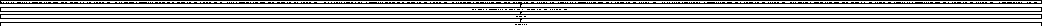
\includegraphics[height=0.347233cm]{structreg_1_1_method}
\end{center}
\end{figure}


\subsection{Detailed Description}


Definition at line 33 of file Registrator.\+h.



The documentation for this struct was generated from the following file\+:\begin{DoxyCompactItemize}
\item 
/home/adam/\+Desktop/reg/\+Registrator/\hyperlink{_registrator_8h}{Registrator.\+h}\end{DoxyCompactItemize}

\hypertarget{structreg_1_1_metric}{}\section{reg\+:\+:Metric Struct Reference}
\label{structreg_1_1_metric}\index{reg\+::\+Metric@{reg\+::\+Metric}}


{\ttfamily \#include $<$Registrator.\+h$>$}

Inheritance diagram for reg\+:\+:Metric\+:\begin{figure}[H]
\begin{center}
\leavevmode
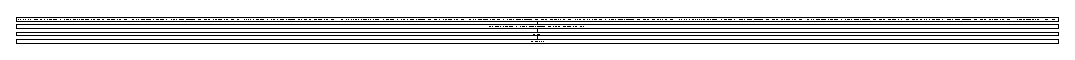
\includegraphics[height=0.352645cm]{structreg_1_1_metric}
\end{center}
\end{figure}


\subsection{Detailed Description}


Definition at line 37 of file Registrator.\+h.



The documentation for this struct was generated from the following file\+:\begin{DoxyCompactItemize}
\item 
/home/adam/\+Desktop/reg/\+Registrator/\hyperlink{_registrator_8h}{Registrator.\+h}\end{DoxyCompactItemize}

\hypertarget{structreg_1_1_monitor}{}\section{reg\+:\+:Monitor Struct Reference}
\label{structreg_1_1_monitor}\index{reg\+::\+Monitor@{reg\+::\+Monitor}}


{\ttfamily \#include $<$Registrator.\+h$>$}

Inheritance diagram for reg\+:\+:Monitor\+:\begin{figure}[H]
\begin{center}
\leavevmode
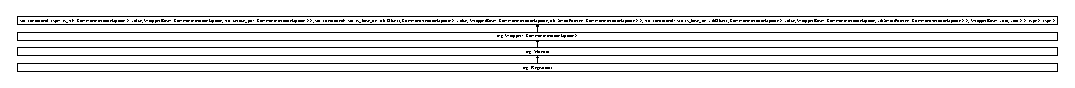
\includegraphics[height=0.732505cm]{structreg_1_1_monitor}
\end{center}
\end{figure}


\subsection{Detailed Description}


Definition at line 55 of file Registrator.\+h.



The documentation for this struct was generated from the following file\+:\begin{DoxyCompactItemize}
\item 
/home/adam/\+Desktop/reg/\+Registrator/\hyperlink{_registrator_8h}{Registrator.\+h}\end{DoxyCompactItemize}

\hypertarget{structreg_1_1_moving}{}\section{reg\+:\+:Moving Struct Reference}
\label{structreg_1_1_moving}\index{reg\+::\+Moving@{reg\+::\+Moving}}


{\ttfamily \#include $<$Registrator.\+h$>$}

Inheritance diagram for reg\+:\+:Moving\+:\begin{figure}[H]
\begin{center}
\leavevmode
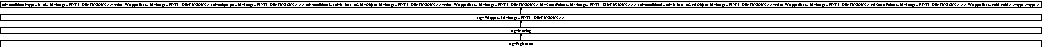
\includegraphics[height=0.625698cm]{structreg_1_1_moving}
\end{center}
\end{figure}


\subsection{Detailed Description}


Definition at line 22 of file Registrator.\+h.



The documentation for this struct was generated from the following file\+:\begin{DoxyCompactItemize}
\item 
/home/adam/\+Desktop/reg/\+Registrator/\hyperlink{_registrator_8h}{Registrator.\+h}\end{DoxyCompactItemize}

\hypertarget{structreg_1_1_optimizer}{}\section{reg\+:\+:Optimizer Struct Reference}
\label{structreg_1_1_optimizer}\index{reg\+::\+Optimizer@{reg\+::\+Optimizer}}


{\ttfamily \#include $<$Registrator.\+h$>$}

Inheritance diagram for reg\+:\+:Optimizer\+:\begin{figure}[H]
\begin{center}
\leavevmode
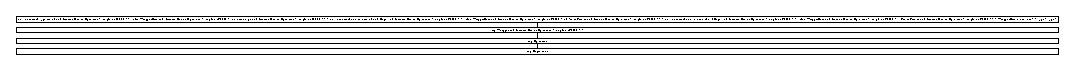
\includegraphics[height=0.509207cm]{structreg_1_1_optimizer}
\end{center}
\end{figure}


\subsection{Detailed Description}


Definition at line 40 of file Registrator.\+h.



The documentation for this struct was generated from the following file\+:\begin{DoxyCompactItemize}
\item 
/home/adam/\+Desktop/reg/\+Registrator/\hyperlink{_registrator_8h}{Registrator.\+h}\end{DoxyCompactItemize}

\hypertarget{structreg_1_1_reader}{}\section{reg\+:\+:Reader Struct Reference}
\label{structreg_1_1_reader}\index{reg\+::\+Reader@{reg\+::\+Reader}}


read an image into itk\+::\+Image$<$double, 3$>$  




{\ttfamily \#include $<$Reader.\+h$>$}

Inheritance diagram for reg\+:\+:Reader\+:\begin{figure}[H]
\begin{center}
\leavevmode
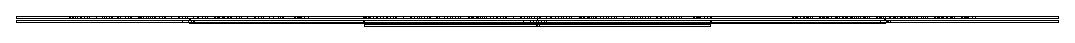
\includegraphics[height=0.133302cm]{structreg_1_1_reader}
\end{center}
\end{figure}
\subsection*{Public Member Functions}
\begin{DoxyCompactItemize}
\item 
\hyperlink{structreg_1_1_reader_abbb5102832a229bb96b75ec5c990b3f3}{Reader} ()=default
\item 
\hyperlink{structreg_1_1_reader_a0c69ac8185cf110c693496eb86c1a734}{Reader} (std\+::string \&\&)
\item 
void \hyperlink{structreg_1_1_reader_a5d87eae44d06ce2e055c6f3cd8b46241}{Execute} (std\+::string \&\&)
\item 
void \hyperlink{structreg_1_1_reader_ac537416d01e0f7ed72506126de45c54c}{Initialize} (std\+::string \&\&)
\end{DoxyCompactItemize}


\subsection{Detailed Description}
read an image into itk\+::\+Image$<$double, 3$>$ 

\begin{DoxyNote}{Note}

\end{DoxyNote}


Definition at line 11 of file Reader.\+h.



\subsection{Constructor \& Destructor Documentation}
\mbox{\Hypertarget{structreg_1_1_reader_abbb5102832a229bb96b75ec5c990b3f3}\label{structreg_1_1_reader_abbb5102832a229bb96b75ec5c990b3f3}} 
\index{reg\+::\+Reader@{reg\+::\+Reader}!Reader@{Reader}}
\index{Reader@{Reader}!reg\+::\+Reader@{reg\+::\+Reader}}
\subsubsection{\texorpdfstring{Reader()}{Reader()}\hspace{0.1cm}{\footnotesize\ttfamily [1/2]}}
{\footnotesize\ttfamily reg\+::\+Reader\+::\+Reader (\begin{DoxyParamCaption}{ }\end{DoxyParamCaption})\hspace{0.3cm}{\ttfamily [default]}}

\mbox{\Hypertarget{structreg_1_1_reader_a0c69ac8185cf110c693496eb86c1a734}\label{structreg_1_1_reader_a0c69ac8185cf110c693496eb86c1a734}} 
\index{reg\+::\+Reader@{reg\+::\+Reader}!Reader@{Reader}}
\index{Reader@{Reader}!reg\+::\+Reader@{reg\+::\+Reader}}
\subsubsection{\texorpdfstring{Reader()}{Reader()}\hspace{0.1cm}{\footnotesize\ttfamily [2/2]}}
{\footnotesize\ttfamily reg\+::\+Reader\+::\+Reader (\begin{DoxyParamCaption}\item[{std\+::string \&\&}]{filename }\end{DoxyParamCaption})}



Definition at line 3 of file Reader.\+cpp.



\subsection{Member Function Documentation}
\mbox{\Hypertarget{structreg_1_1_reader_a5d87eae44d06ce2e055c6f3cd8b46241}\label{structreg_1_1_reader_a5d87eae44d06ce2e055c6f3cd8b46241}} 
\index{reg\+::\+Reader@{reg\+::\+Reader}!Execute@{Execute}}
\index{Execute@{Execute}!reg\+::\+Reader@{reg\+::\+Reader}}
\subsubsection{\texorpdfstring{Execute()}{Execute()}}
{\footnotesize\ttfamily void reg\+::\+Reader\+::\+Execute (\begin{DoxyParamCaption}\item[{std\+::string \&\&}]{filename }\end{DoxyParamCaption})}



Definition at line 8 of file Reader.\+cpp.

\mbox{\Hypertarget{structreg_1_1_reader_ac537416d01e0f7ed72506126de45c54c}\label{structreg_1_1_reader_ac537416d01e0f7ed72506126de45c54c}} 
\index{reg\+::\+Reader@{reg\+::\+Reader}!Initialize@{Initialize}}
\index{Initialize@{Initialize}!reg\+::\+Reader@{reg\+::\+Reader}}
\subsubsection{\texorpdfstring{Initialize()}{Initialize()}}
{\footnotesize\ttfamily void reg\+::\+Reader\+::\+Initialize (\begin{DoxyParamCaption}\item[{std\+::string \&\&}]{filename }\end{DoxyParamCaption})}



Definition at line 16 of file Reader.\+cpp.



The documentation for this struct was generated from the following files\+:\begin{DoxyCompactItemize}
\item 
/home/adam/\+Desktop/reg/\+Reader/\hyperlink{_reader_8h}{Reader.\+h}\item 
/home/adam/\+Desktop/reg/\+Reader/\hyperlink{_reader_8cpp}{Reader.\+cpp}\end{DoxyCompactItemize}

\hypertarget{structreg_1_1_registrator}{}\section{reg\+:\+:Registrator Struct Reference}
\label{structreg_1_1_registrator}\index{reg\+::\+Registrator@{reg\+::\+Registrator}}


{\ttfamily \#include $<$Registrator.\+h$>$}

Inheritance diagram for reg\+:\+:Registrator\+:\begin{figure}[H]
\begin{center}
\leavevmode
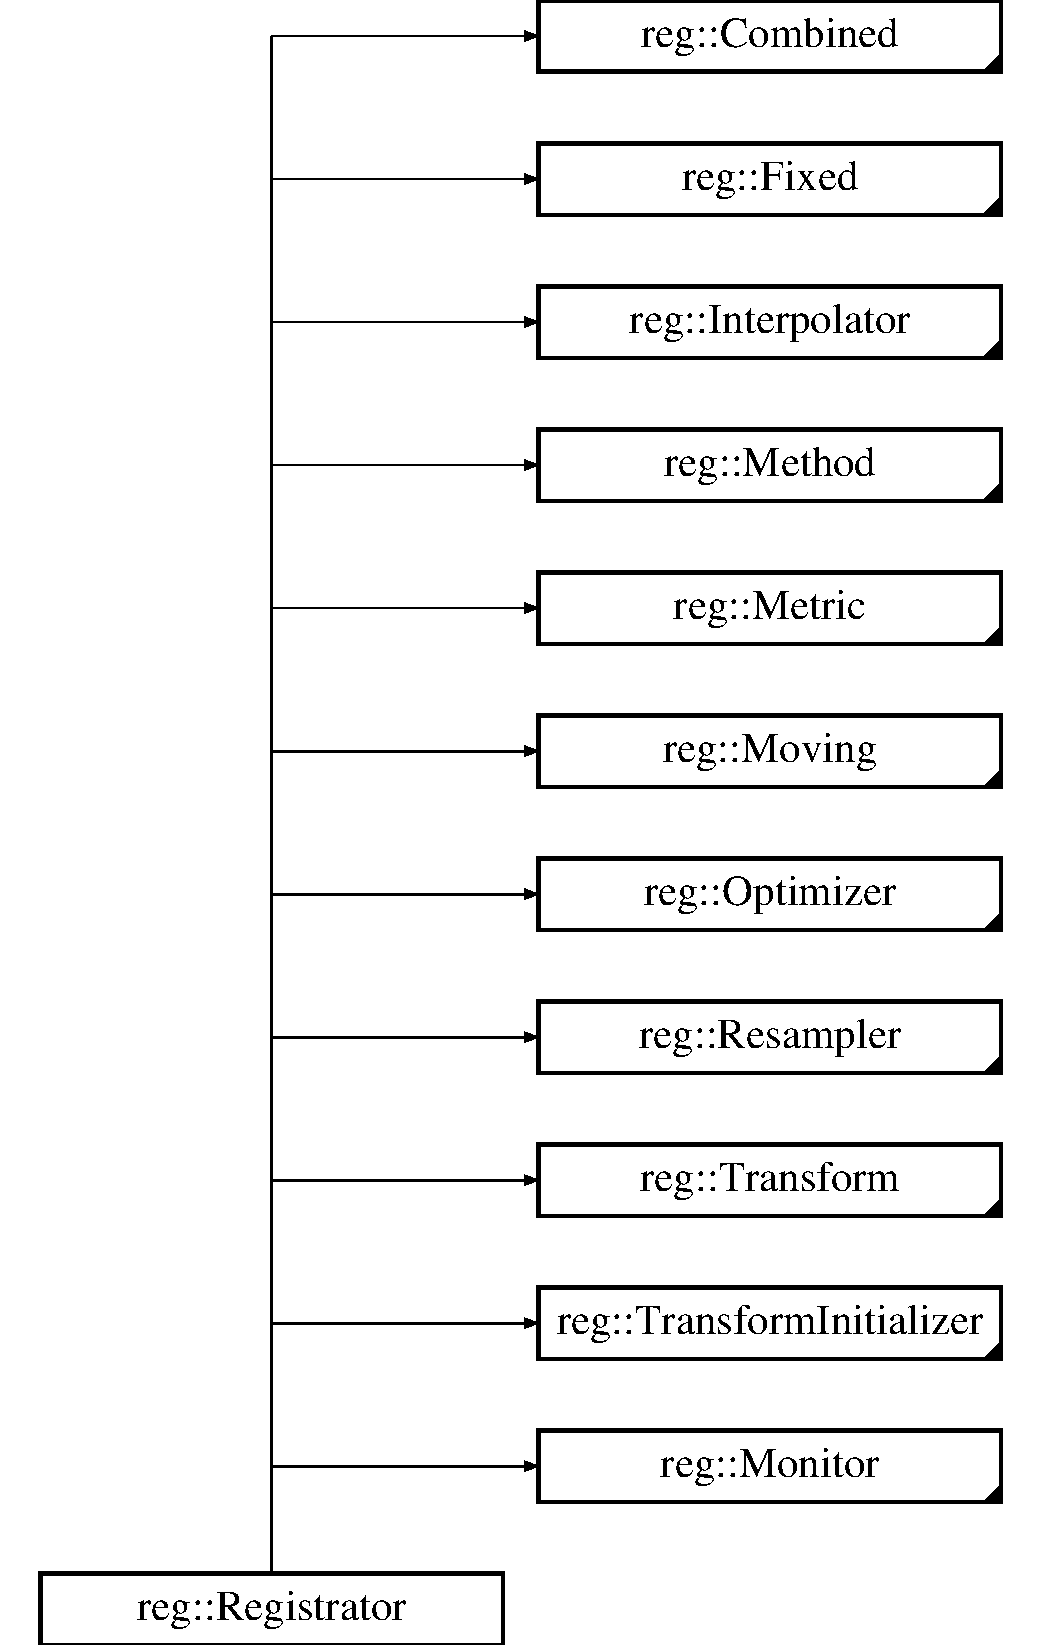
\includegraphics[height=12.000000cm]{structreg_1_1_registrator}
\end{center}
\end{figure}
\subsection*{Public Member Functions}
\begin{DoxyCompactItemize}
\item 
\hyperlink{structreg_1_1_registrator_a0a8d44017cb8112001a1d13f984145ef}{Registrator} ()=default
\item 
\hyperlink{structreg_1_1_registrator_a63b1984827ba8ccbbc785502bbc3c5da}{Registrator} (Fixed\+::self\+\_\+type $\ast$, Moving\+::self\+\_\+type $\ast$)
\item 
void \hyperlink{structreg_1_1_registrator_a8415aef78761d11e560d280ce30f0de8}{Initialize} (Fixed\+::self\+\_\+type $\ast$, Moving\+::self\+\_\+type $\ast$)
\item 
void \hyperlink{structreg_1_1_registrator_ac8709c0e86e8e53bffc04ae517bdb863}{Execute} (Fixed\+::self\+\_\+type $\ast$, Moving\+::self\+\_\+type $\ast$)
\end{DoxyCompactItemize}


\subsection{Detailed Description}


Definition at line 57 of file Registrator.\+h.



\subsection{Constructor \& Destructor Documentation}
\mbox{\Hypertarget{structreg_1_1_registrator_a0a8d44017cb8112001a1d13f984145ef}\label{structreg_1_1_registrator_a0a8d44017cb8112001a1d13f984145ef}} 
\index{reg\+::\+Registrator@{reg\+::\+Registrator}!Registrator@{Registrator}}
\index{Registrator@{Registrator}!reg\+::\+Registrator@{reg\+::\+Registrator}}
\subsubsection{\texorpdfstring{Registrator()}{Registrator()}\hspace{0.1cm}{\footnotesize\ttfamily [1/2]}}
{\footnotesize\ttfamily reg\+::\+Registrator\+::\+Registrator (\begin{DoxyParamCaption}{ }\end{DoxyParamCaption})\hspace{0.3cm}{\ttfamily [default]}}

\mbox{\Hypertarget{structreg_1_1_registrator_a63b1984827ba8ccbbc785502bbc3c5da}\label{structreg_1_1_registrator_a63b1984827ba8ccbbc785502bbc3c5da}} 
\index{reg\+::\+Registrator@{reg\+::\+Registrator}!Registrator@{Registrator}}
\index{Registrator@{Registrator}!reg\+::\+Registrator@{reg\+::\+Registrator}}
\subsubsection{\texorpdfstring{Registrator()}{Registrator()}\hspace{0.1cm}{\footnotesize\ttfamily [2/2]}}
{\footnotesize\ttfamily reg\+::\+Registrator\+::\+Registrator (\begin{DoxyParamCaption}\item[{Fixed\+::self\+\_\+type $\ast$}]{fixed,  }\item[{Moving\+::self\+\_\+type $\ast$}]{moving }\end{DoxyParamCaption})}



Definition at line 3 of file Registrator.\+cpp.



\subsection{Member Function Documentation}
\mbox{\Hypertarget{structreg_1_1_registrator_ac8709c0e86e8e53bffc04ae517bdb863}\label{structreg_1_1_registrator_ac8709c0e86e8e53bffc04ae517bdb863}} 
\index{reg\+::\+Registrator@{reg\+::\+Registrator}!Execute@{Execute}}
\index{Execute@{Execute}!reg\+::\+Registrator@{reg\+::\+Registrator}}
\subsubsection{\texorpdfstring{Execute()}{Execute()}}
{\footnotesize\ttfamily void reg\+::\+Registrator\+::\+Execute (\begin{DoxyParamCaption}\item[{Fixed\+::self\+\_\+type $\ast$}]{fixed,  }\item[{Moving\+::self\+\_\+type $\ast$}]{moving }\end{DoxyParamCaption})}



Definition at line 23 of file Registrator.\+cpp.

\mbox{\Hypertarget{structreg_1_1_registrator_a8415aef78761d11e560d280ce30f0de8}\label{structreg_1_1_registrator_a8415aef78761d11e560d280ce30f0de8}} 
\index{reg\+::\+Registrator@{reg\+::\+Registrator}!Initialize@{Initialize}}
\index{Initialize@{Initialize}!reg\+::\+Registrator@{reg\+::\+Registrator}}
\subsubsection{\texorpdfstring{Initialize()}{Initialize()}}
{\footnotesize\ttfamily void reg\+::\+Registrator\+::\+Initialize (\begin{DoxyParamCaption}\item[{Fixed\+::self\+\_\+type $\ast$}]{fixed,  }\item[{Moving\+::self\+\_\+type $\ast$}]{moving }\end{DoxyParamCaption})}



Definition at line 9 of file Registrator.\+cpp.



The documentation for this struct was generated from the following files\+:\begin{DoxyCompactItemize}
\item 
/home/adam/\+Desktop/reg/\+Registrator/\hyperlink{_registrator_8h}{Registrator.\+h}\item 
/home/adam/\+Desktop/reg/\+Registrator/\hyperlink{_registrator_8cpp}{Registrator.\+cpp}\end{DoxyCompactItemize}

\hypertarget{structreg_1_1_resampler}{}\section{reg\+:\+:Resampler Struct Reference}
\label{structreg_1_1_resampler}\index{reg\+::\+Resampler@{reg\+::\+Resampler}}


{\ttfamily \#include $<$Registrator.\+h$>$}

Inheritance diagram for reg\+:\+:Resampler\+:\begin{figure}[H]
\begin{center}
\leavevmode
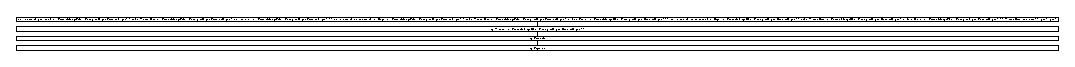
\includegraphics[height=0.448628cm]{structreg_1_1_resampler}
\end{center}
\end{figure}


\subsection{Detailed Description}
$<$ \begin{DoxyNote}{Note}
optional template parameters not explicitly declared 
\end{DoxyNote}


Definition at line 42 of file Registrator.\+h.



The documentation for this struct was generated from the following file\+:\begin{DoxyCompactItemize}
\item 
/home/adam/\+Desktop/reg/\+Registrator/\hyperlink{_registrator_8h}{Registrator.\+h}\end{DoxyCompactItemize}

\hypertarget{structreg_1_1_transform}{}\section{reg\+:\+:Transform Struct Reference}
\label{structreg_1_1_transform}\index{reg\+::\+Transform@{reg\+::\+Transform}}


{\ttfamily \#include $<$Registrator.\+h$>$}

Inheritance diagram for reg\+:\+:Transform\+:\begin{figure}[H]
\begin{center}
\leavevmode
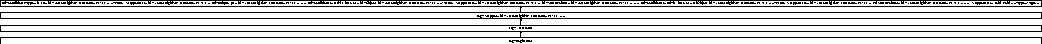
\includegraphics[height=0.595745cm]{structreg_1_1_transform}
\end{center}
\end{figure}


\subsection{Detailed Description}
$<$ \begin{DoxyWarning}{Warning}
require manipulation when changing D\+I\+M\+E\+N\+S\+I\+O\+NS 
\end{DoxyWarning}


Definition at line 24 of file Registrator.\+h.



The documentation for this struct was generated from the following file\+:\begin{DoxyCompactItemize}
\item 
/home/adam/\+Desktop/reg/\+Registrator/\hyperlink{_registrator_8h}{Registrator.\+h}\end{DoxyCompactItemize}

\hypertarget{structreg_1_1_transform_initializer}{}\section{reg\+:\+:Transform\+Initializer Struct Reference}
\label{structreg_1_1_transform_initializer}\index{reg\+::\+Transform\+Initializer@{reg\+::\+Transform\+Initializer}}


{\ttfamily \#include $<$Registrator.\+h$>$}

Inheritance diagram for reg\+:\+:Transform\+Initializer\+:\begin{figure}[H]
\begin{center}
\leavevmode
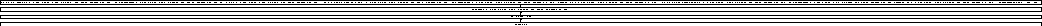
\includegraphics[height=0.345306cm]{structreg_1_1_transform_initializer}
\end{center}
\end{figure}


\subsection{Detailed Description}


Definition at line 51 of file Registrator.\+h.



The documentation for this struct was generated from the following file\+:\begin{DoxyCompactItemize}
\item 
/home/adam/\+Desktop/reg/\+Registrator/\hyperlink{_registrator_8h}{Registrator.\+h}\end{DoxyCompactItemize}

\hypertarget{classitk_1_1_transform_i_o_factory_register_manager}{}\section{itk\+:\+:Transform\+I\+O\+Factory\+Register\+Manager Class Reference}
\label{classitk_1_1_transform_i_o_factory_register_manager}\index{itk\+::\+Transform\+I\+O\+Factory\+Register\+Manager@{itk\+::\+Transform\+I\+O\+Factory\+Register\+Manager}}


{\ttfamily \#include $<$itk\+Transform\+I\+O\+Factory\+Register\+Manager.\+h$>$}

\subsection*{Public Member Functions}
\begin{DoxyCompactItemize}
\item 
\hyperlink{classitk_1_1_transform_i_o_factory_register_manager_aefb761ca3bfca773fe91c4861c19e4f8}{Transform\+I\+O\+Factory\+Register\+Manager} (void($\ast$list\mbox{[}$\,$\mbox{]})(void))
\item 
\hyperlink{classitk_1_1_transform_i_o_factory_register_manager_aefb761ca3bfca773fe91c4861c19e4f8}{Transform\+I\+O\+Factory\+Register\+Manager} (void($\ast$list\mbox{[}$\,$\mbox{]})(void))
\end{DoxyCompactItemize}


\subsection{Detailed Description}


Definition at line 24 of file itk\+Transform\+I\+O\+Factory\+Register\+Manager.\+h.



\subsection{Constructor \& Destructor Documentation}
\mbox{\Hypertarget{classitk_1_1_transform_i_o_factory_register_manager_aefb761ca3bfca773fe91c4861c19e4f8}\label{classitk_1_1_transform_i_o_factory_register_manager_aefb761ca3bfca773fe91c4861c19e4f8}} 
\index{itk\+::\+Transform\+I\+O\+Factory\+Register\+Manager@{itk\+::\+Transform\+I\+O\+Factory\+Register\+Manager}!Transform\+I\+O\+Factory\+Register\+Manager@{Transform\+I\+O\+Factory\+Register\+Manager}}
\index{Transform\+I\+O\+Factory\+Register\+Manager@{Transform\+I\+O\+Factory\+Register\+Manager}!itk\+::\+Transform\+I\+O\+Factory\+Register\+Manager@{itk\+::\+Transform\+I\+O\+Factory\+Register\+Manager}}
\subsubsection{\texorpdfstring{Transform\+I\+O\+Factory\+Register\+Manager()}{TransformIOFactoryRegisterManager()}\hspace{0.1cm}{\footnotesize\ttfamily [1/2]}}
{\footnotesize\ttfamily itk\+::\+Transform\+I\+O\+Factory\+Register\+Manager\+::\+Transform\+I\+O\+Factory\+Register\+Manager (\begin{DoxyParamCaption}\item[{void($\ast$\mbox{[}$\,$\mbox{]})(void)}]{list }\end{DoxyParamCaption})\hspace{0.3cm}{\ttfamily [inline]}}



Definition at line 27 of file itk\+Transform\+I\+O\+Factory\+Register\+Manager.\+h.

\mbox{\Hypertarget{classitk_1_1_transform_i_o_factory_register_manager_aefb761ca3bfca773fe91c4861c19e4f8}\label{classitk_1_1_transform_i_o_factory_register_manager_aefb761ca3bfca773fe91c4861c19e4f8}} 
\index{itk\+::\+Transform\+I\+O\+Factory\+Register\+Manager@{itk\+::\+Transform\+I\+O\+Factory\+Register\+Manager}!Transform\+I\+O\+Factory\+Register\+Manager@{Transform\+I\+O\+Factory\+Register\+Manager}}
\index{Transform\+I\+O\+Factory\+Register\+Manager@{Transform\+I\+O\+Factory\+Register\+Manager}!itk\+::\+Transform\+I\+O\+Factory\+Register\+Manager@{itk\+::\+Transform\+I\+O\+Factory\+Register\+Manager}}
\subsubsection{\texorpdfstring{Transform\+I\+O\+Factory\+Register\+Manager()}{TransformIOFactoryRegisterManager()}\hspace{0.1cm}{\footnotesize\ttfamily [2/2]}}
{\footnotesize\ttfamily itk\+::\+Transform\+I\+O\+Factory\+Register\+Manager\+::\+Transform\+I\+O\+Factory\+Register\+Manager (\begin{DoxyParamCaption}\item[{void($\ast$\mbox{[}$\,$\mbox{]})(void)}]{list }\end{DoxyParamCaption})\hspace{0.3cm}{\ttfamily [inline]}}



Definition at line 27 of file itk\+Transform\+I\+O\+Factory\+Register\+Manager.\+h.



The documentation for this class was generated from the following file\+:\begin{DoxyCompactItemize}
\item 
/home/adam/\+Desktop/reg/build/\+I\+T\+K\+I\+O\+Factory\+Registration/\hyperlink{build_2_i_t_k_i_o_factory_registration_2itk_transform_i_o_factory_register_manager_8h}{itk\+Transform\+I\+O\+Factory\+Register\+Manager.\+h}\end{DoxyCompactItemize}

\hypertarget{structreg_1_1_visualizer}{}\section{reg\+:\+:Visualizer Struct Reference}
\label{structreg_1_1_visualizer}\index{reg\+::\+Visualizer@{reg\+::\+Visualizer}}


visualize vtk\+Image\+Data in 3D space  




{\ttfamily \#include $<$Visualizer.\+h$>$}

Inheritance diagram for reg\+:\+:Visualizer\+:\begin{figure}[H]
\begin{center}
\leavevmode
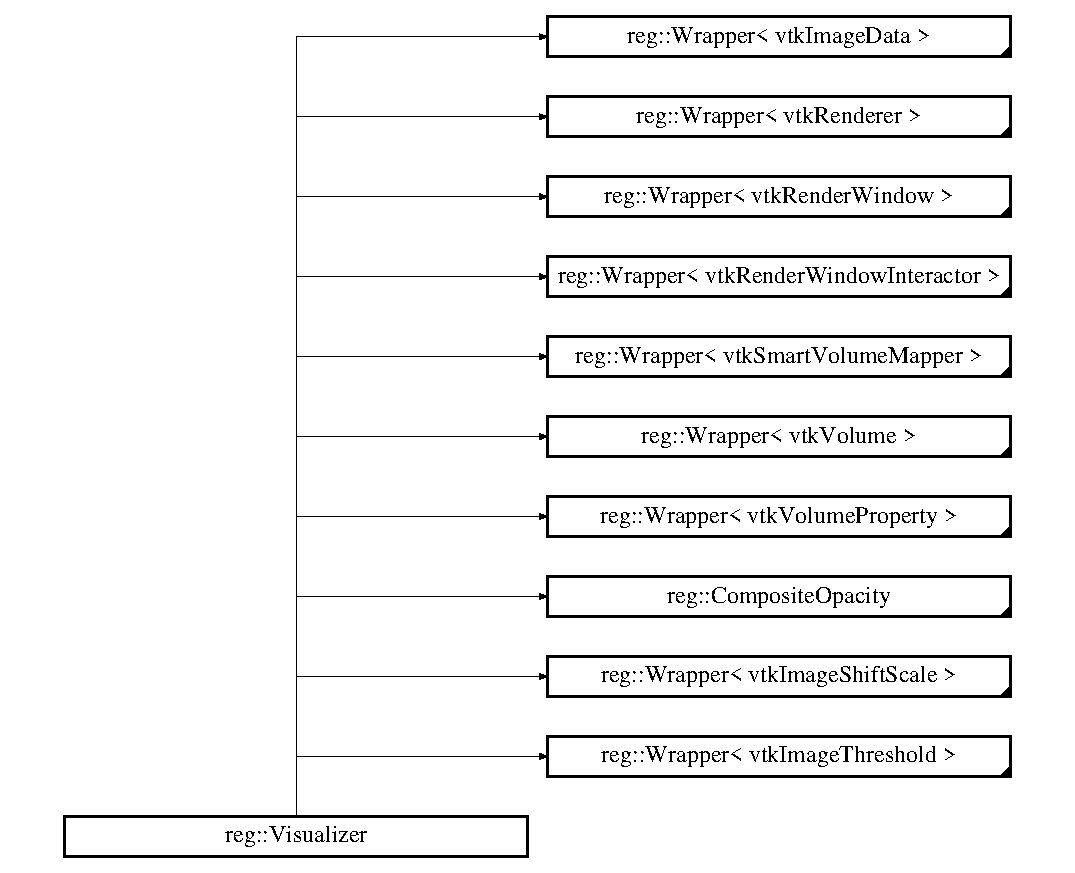
\includegraphics[height=11.000000cm]{structreg_1_1_visualizer}
\end{center}
\end{figure}
\subsection*{Public Member Functions}
\begin{DoxyCompactItemize}
\item 
\hyperlink{structreg_1_1_visualizer_a7b2aa4228668fdd9e9c174fc060d2fb9}{Visualizer} ()=default
\item 
\hyperlink{structreg_1_1_visualizer_a0746fc30028f0293bedd23468dae4d43}{Visualizer} (vtk\+Image\+Data $\ast$)
\item 
void \hyperlink{structreg_1_1_visualizer_aad11952fc8c47d0f208620a690ce4985}{Execute} (vtk\+Image\+Data $\ast$)
\item 
void \hyperlink{structreg_1_1_visualizer_a43f723595f4d7c1043cc13997aa9046b}{Initialize} (vtk\+Image\+Data $\ast$)
\end{DoxyCompactItemize}


\subsection{Detailed Description}
visualize vtk\+Image\+Data in 3D space 

Definition at line 22 of file Visualizer.\+h.



\subsection{Constructor \& Destructor Documentation}
\mbox{\Hypertarget{structreg_1_1_visualizer_a7b2aa4228668fdd9e9c174fc060d2fb9}\label{structreg_1_1_visualizer_a7b2aa4228668fdd9e9c174fc060d2fb9}} 
\index{reg\+::\+Visualizer@{reg\+::\+Visualizer}!Visualizer@{Visualizer}}
\index{Visualizer@{Visualizer}!reg\+::\+Visualizer@{reg\+::\+Visualizer}}
\subsubsection{\texorpdfstring{Visualizer()}{Visualizer()}\hspace{0.1cm}{\footnotesize\ttfamily [1/2]}}
{\footnotesize\ttfamily reg\+::\+Visualizer\+::\+Visualizer (\begin{DoxyParamCaption}{ }\end{DoxyParamCaption})\hspace{0.3cm}{\ttfamily [default]}}

\mbox{\Hypertarget{structreg_1_1_visualizer_a0746fc30028f0293bedd23468dae4d43}\label{structreg_1_1_visualizer_a0746fc30028f0293bedd23468dae4d43}} 
\index{reg\+::\+Visualizer@{reg\+::\+Visualizer}!Visualizer@{Visualizer}}
\index{Visualizer@{Visualizer}!reg\+::\+Visualizer@{reg\+::\+Visualizer}}
\subsubsection{\texorpdfstring{Visualizer()}{Visualizer()}\hspace{0.1cm}{\footnotesize\ttfamily [2/2]}}
{\footnotesize\ttfamily reg\+::\+Visualizer\+::\+Visualizer (\begin{DoxyParamCaption}\item[{vtk\+Image\+Data $\ast$}]{image }\end{DoxyParamCaption})}



Definition at line 3 of file Visualizer.\+cpp.



\subsection{Member Function Documentation}
\mbox{\Hypertarget{structreg_1_1_visualizer_aad11952fc8c47d0f208620a690ce4985}\label{structreg_1_1_visualizer_aad11952fc8c47d0f208620a690ce4985}} 
\index{reg\+::\+Visualizer@{reg\+::\+Visualizer}!Execute@{Execute}}
\index{Execute@{Execute}!reg\+::\+Visualizer@{reg\+::\+Visualizer}}
\subsubsection{\texorpdfstring{Execute()}{Execute()}}
{\footnotesize\ttfamily void reg\+::\+Visualizer\+::\+Execute (\begin{DoxyParamCaption}\item[{vtk\+Image\+Data $\ast$}]{image }\end{DoxyParamCaption})}

$<$ increase brightness by a factor of 5

$<$ inclusive range of grey values

$<$ specify replace values not in inclusive range

$<$ set non-\/included values to 0

$<$ explicitly specify no opacity 

Definition at line 8 of file Visualizer.\+cpp.

\mbox{\Hypertarget{structreg_1_1_visualizer_a43f723595f4d7c1043cc13997aa9046b}\label{structreg_1_1_visualizer_a43f723595f4d7c1043cc13997aa9046b}} 
\index{reg\+::\+Visualizer@{reg\+::\+Visualizer}!Initialize@{Initialize}}
\index{Initialize@{Initialize}!reg\+::\+Visualizer@{reg\+::\+Visualizer}}
\subsubsection{\texorpdfstring{Initialize()}{Initialize()}}
{\footnotesize\ttfamily void reg\+::\+Visualizer\+::\+Initialize (\begin{DoxyParamCaption}\item[{vtk\+Image\+Data $\ast$}]{image }\end{DoxyParamCaption})}



Definition at line 47 of file Visualizer.\+cpp.



The documentation for this struct was generated from the following files\+:\begin{DoxyCompactItemize}
\item 
/home/adam/\+Desktop/reg/\+Visualizer/\hyperlink{_visualizer_8h}{Visualizer.\+h}\item 
/home/adam/\+Desktop/reg/\+Visualizer/\hyperlink{_visualizer_8cpp}{Visualizer.\+cpp}\end{DoxyCompactItemize}

\hypertarget{structreg_1_1_wrapper}{}\section{reg\+:\+:Wrapper$<$ T $>$ Struct Template Reference}
\label{structreg_1_1_wrapper}\index{reg\+::\+Wrapper$<$ T $>$@{reg\+::\+Wrapper$<$ T $>$}}


interface \hyperlink{structreg_1_1_wrapper}{Wrapper}  




{\ttfamily \#include $<$Wrapper.\+h$>$}

Inheritance diagram for reg\+:\+:Wrapper$<$ T $>$\+:\begin{figure}[H]
\begin{center}
\leavevmode
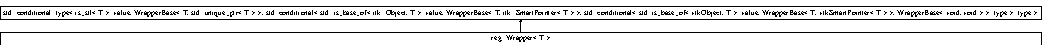
\includegraphics[height=0.598930cm]{structreg_1_1_wrapper}
\end{center}
\end{figure}


\subsection{Detailed Description}
\subsubsection*{template$<$typename T$>$\newline
struct reg\+::\+Wrapper$<$ T $>$}

interface \hyperlink{structreg_1_1_wrapper}{Wrapper} 

chooses which \hyperlink{structreg_1_1_wrapper_base}{Wrapper\+Base} to inherit depending on {\ttfamily T} \begin{DoxyWarning}{Warning}
not optimized for extensibility 
\end{DoxyWarning}
\begin{DoxyNote}{Note}
possible future implementation using S\+F\+I\+N\+AE and void\+\_\+t 
\end{DoxyNote}

\begin{DoxyParams}{Parameters}
{\em T} & contained type \\
\hline
\end{DoxyParams}


Definition at line 114 of file Wrapper.\+h.



The documentation for this struct was generated from the following file\+:\begin{DoxyCompactItemize}
\item 
/home/adam/\+Desktop/reg/\+Wrapper/\hyperlink{_wrapper_8h}{Wrapper.\+h}\end{DoxyCompactItemize}

\hypertarget{structreg_1_1_wrapper_base}{}\section{reg\+:\+:Wrapper\+Base$<$ typename, typename $>$ Struct Template Reference}
\label{structreg_1_1_wrapper_base}\index{reg\+::\+Wrapper\+Base$<$ typename, typename $>$@{reg\+::\+Wrapper\+Base$<$ typename, typename $>$}}


general template of \hyperlink{structreg_1_1_wrapper_base}{Wrapper\+Base}  




{\ttfamily \#include $<$Wrapper.\+h$>$}

Inheritance diagram for reg\+:\+:Wrapper\+Base$<$ typename, typename $>$\+:\begin{figure}[H]
\begin{center}
\leavevmode
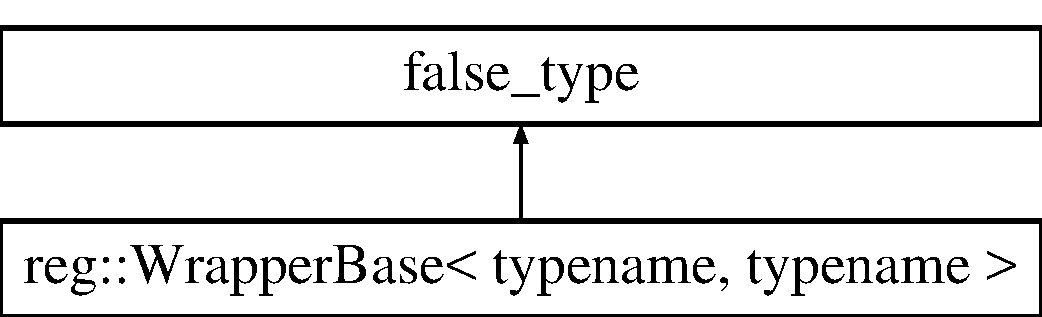
\includegraphics[height=2.000000cm]{structreg_1_1_wrapper_base}
\end{center}
\end{figure}


\subsection{Detailed Description}
\subsubsection*{template$<$typename, typename$>$\newline
struct reg\+::\+Wrapper\+Base$<$ typename, typename $>$}

general template of \hyperlink{structreg_1_1_wrapper_base}{Wrapper\+Base} 

specialized template of \hyperlink{structreg_1_1_wrapper_base}{Wrapper\+Base}

$<$ check if \hyperlink{structreg_1_1_wrapper}{Wrapper} inherits any specialized \hyperlink{structreg_1_1_wrapper_base}{Wrapper\+Base} structs

\begin{DoxyNote}{Note}
not specialized 
\end{DoxyNote}
\begin{DoxyWarning}{Warning}
not meant to be selected as Base
\end{DoxyWarning}
specialized for types in S\+TL 
\begin{DoxyParams}{Parameters}
{\em T} & contained type\\
\hline
\end{DoxyParams}
specialized for types in itk 
\begin{DoxyParams}{Parameters}
{\em T} & contained type\\
\hline
\end{DoxyParams}
specialized for types in vtk 
\begin{DoxyParams}{Parameters}
{\em T} & contained type \\
\hline
\end{DoxyParams}


Definition at line 43 of file Wrapper.\+h.



The documentation for this struct was generated from the following file\+:\begin{DoxyCompactItemize}
\item 
/home/adam/\+Desktop/reg/\+Wrapper/\hyperlink{_wrapper_8h}{Wrapper.\+h}\end{DoxyCompactItemize}

\hypertarget{structreg_1_1_wrapper_base_3_01_t_00_01itk_1_1_smart_pointer_3_01_t_01_4_01_4}{}\section{reg\+:\+:Wrapper\+Base$<$ T, itk\+:\+:Smart\+Pointer$<$ T $>$ $>$ Struct Template Reference}
\label{structreg_1_1_wrapper_base_3_01_t_00_01itk_1_1_smart_pointer_3_01_t_01_4_01_4}\index{reg\+::\+Wrapper\+Base$<$ T, itk\+::\+Smart\+Pointer$<$ T $>$ $>$@{reg\+::\+Wrapper\+Base$<$ T, itk\+::\+Smart\+Pointer$<$ T $>$ $>$}}


{\ttfamily \#include $<$Wrapper.\+h$>$}

Inheritance diagram for reg\+:\+:Wrapper\+Base$<$ T, itk\+:\+:Smart\+Pointer$<$ T $>$ $>$\+:\begin{figure}[H]
\begin{center}
\leavevmode
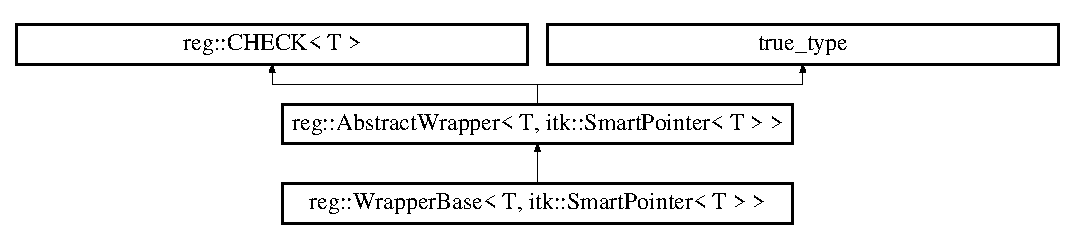
\includegraphics[height=2.781457cm]{structreg_1_1_wrapper_base_3_01_t_00_01itk_1_1_smart_pointer_3_01_t_01_4_01_4}
\end{center}
\end{figure}
\subsection*{Public Member Functions}
\begin{DoxyCompactItemize}
\item 
T $\ast$ \hyperlink{structreg_1_1_wrapper_base_3_01_t_00_01itk_1_1_smart_pointer_3_01_t_01_4_01_4_ac2d57c43556c87aa45dcafd2c8a9cb47}{Get} () const noexcept override
\item 
void \hyperlink{structreg_1_1_wrapper_base_3_01_t_00_01itk_1_1_smart_pointer_3_01_t_01_4_01_4_a9a9bcfbe7236f66cb355f929aeeca281}{Set} (T $\ast$) noexcept override
\end{DoxyCompactItemize}
\subsection*{Protected Member Functions}
\begin{DoxyCompactItemize}
\item 
void \hyperlink{structreg_1_1_wrapper_base_3_01_t_00_01itk_1_1_smart_pointer_3_01_t_01_4_01_4_a10fb689e5da772970c04d312d600868d}{Allocate} () noexcept override
\end{DoxyCompactItemize}
\subsection*{Additional Inherited Members}


\subsection{Detailed Description}
\subsubsection*{template$<$typename T$>$\newline
struct reg\+::\+Wrapper\+Base$<$ T, itk\+::\+Smart\+Pointer$<$ T $>$ $>$}



Definition at line 66 of file Wrapper.\+h.



\subsection{Member Function Documentation}
\mbox{\Hypertarget{structreg_1_1_wrapper_base_3_01_t_00_01itk_1_1_smart_pointer_3_01_t_01_4_01_4_a10fb689e5da772970c04d312d600868d}\label{structreg_1_1_wrapper_base_3_01_t_00_01itk_1_1_smart_pointer_3_01_t_01_4_01_4_a10fb689e5da772970c04d312d600868d}} 
\index{reg\+::\+Wrapper\+Base$<$ T, itk\+::\+Smart\+Pointer$<$ T $>$ $>$@{reg\+::\+Wrapper\+Base$<$ T, itk\+::\+Smart\+Pointer$<$ T $>$ $>$}!Allocate@{Allocate}}
\index{Allocate@{Allocate}!reg\+::\+Wrapper\+Base$<$ T, itk\+::\+Smart\+Pointer$<$ T $>$ $>$@{reg\+::\+Wrapper\+Base$<$ T, itk\+::\+Smart\+Pointer$<$ T $>$ $>$}}
\subsubsection{\texorpdfstring{Allocate()}{Allocate()}}
{\footnotesize\ttfamily template$<$typename T $>$ \\
void \hyperlink{structreg_1_1_wrapper_base}{reg\+::\+Wrapper\+Base}$<$ T, itk\+::\+Smart\+Pointer$<$ T $>$ $>$\+::Allocate (\begin{DoxyParamCaption}{ }\end{DoxyParamCaption})\hspace{0.3cm}{\ttfamily [inline]}, {\ttfamily [override]}, {\ttfamily [protected]}, {\ttfamily [virtual]}, {\ttfamily [noexcept]}}



Implements \hyperlink{structreg_1_1_abstract_wrapper_aad461ca147a0a7fcfd4f8662994742f3}{reg\+::\+Abstract\+Wrapper$<$ T, itk\+::\+Smart\+Pointer$<$ T $>$ $>$}.



Definition at line 187 of file Wrapper.\+h.

\mbox{\Hypertarget{structreg_1_1_wrapper_base_3_01_t_00_01itk_1_1_smart_pointer_3_01_t_01_4_01_4_ac2d57c43556c87aa45dcafd2c8a9cb47}\label{structreg_1_1_wrapper_base_3_01_t_00_01itk_1_1_smart_pointer_3_01_t_01_4_01_4_ac2d57c43556c87aa45dcafd2c8a9cb47}} 
\index{reg\+::\+Wrapper\+Base$<$ T, itk\+::\+Smart\+Pointer$<$ T $>$ $>$@{reg\+::\+Wrapper\+Base$<$ T, itk\+::\+Smart\+Pointer$<$ T $>$ $>$}!Get@{Get}}
\index{Get@{Get}!reg\+::\+Wrapper\+Base$<$ T, itk\+::\+Smart\+Pointer$<$ T $>$ $>$@{reg\+::\+Wrapper\+Base$<$ T, itk\+::\+Smart\+Pointer$<$ T $>$ $>$}}
\subsubsection{\texorpdfstring{Get()}{Get()}}
{\footnotesize\ttfamily template$<$typename T $>$ \\
T $\ast$ \hyperlink{structreg_1_1_wrapper_base}{reg\+::\+Wrapper\+Base}$<$ T, itk\+::\+Smart\+Pointer$<$ T $>$ $>$\+::Get (\begin{DoxyParamCaption}{ }\end{DoxyParamCaption}) const\hspace{0.3cm}{\ttfamily [inline]}, {\ttfamily [override]}, {\ttfamily [virtual]}, {\ttfamily [noexcept]}}



Implements \hyperlink{structreg_1_1_abstract_wrapper_a88e7079432573b09a5cd695be34e9147}{reg\+::\+Abstract\+Wrapper$<$ T, itk\+::\+Smart\+Pointer$<$ T $>$ $>$}.



Definition at line 133 of file Wrapper.\+h.

\mbox{\Hypertarget{structreg_1_1_wrapper_base_3_01_t_00_01itk_1_1_smart_pointer_3_01_t_01_4_01_4_a9a9bcfbe7236f66cb355f929aeeca281}\label{structreg_1_1_wrapper_base_3_01_t_00_01itk_1_1_smart_pointer_3_01_t_01_4_01_4_a9a9bcfbe7236f66cb355f929aeeca281}} 
\index{reg\+::\+Wrapper\+Base$<$ T, itk\+::\+Smart\+Pointer$<$ T $>$ $>$@{reg\+::\+Wrapper\+Base$<$ T, itk\+::\+Smart\+Pointer$<$ T $>$ $>$}!Set@{Set}}
\index{Set@{Set}!reg\+::\+Wrapper\+Base$<$ T, itk\+::\+Smart\+Pointer$<$ T $>$ $>$@{reg\+::\+Wrapper\+Base$<$ T, itk\+::\+Smart\+Pointer$<$ T $>$ $>$}}
\subsubsection{\texorpdfstring{Set()}{Set()}}
{\footnotesize\ttfamily template$<$typename T $>$ \\
void \hyperlink{structreg_1_1_wrapper_base}{reg\+::\+Wrapper\+Base}$<$ T, itk\+::\+Smart\+Pointer$<$ T $>$ $>$\+::Set (\begin{DoxyParamCaption}\item[{T $\ast$}]{m }\end{DoxyParamCaption})\hspace{0.3cm}{\ttfamily [inline]}, {\ttfamily [override]}, {\ttfamily [virtual]}, {\ttfamily [noexcept]}}



Implements \hyperlink{structreg_1_1_abstract_wrapper_af017f2af039fd5b940345e930e4bb397}{reg\+::\+Abstract\+Wrapper$<$ T, itk\+::\+Smart\+Pointer$<$ T $>$ $>$}.



Definition at line 160 of file Wrapper.\+h.



The documentation for this struct was generated from the following file\+:\begin{DoxyCompactItemize}
\item 
/home/adam/\+Desktop/reg/\+Wrapper/\hyperlink{_wrapper_8h}{Wrapper.\+h}\end{DoxyCompactItemize}

\hypertarget{structreg_1_1_wrapper_base_3_01_t_00_01std_1_1unique__ptr_3_01_t_01_4_01_4}{}\section{reg\+:\+:Wrapper\+Base$<$ T, std\+:\+:unique\+\_\+ptr$<$ T $>$ $>$ Struct Template Reference}
\label{structreg_1_1_wrapper_base_3_01_t_00_01std_1_1unique__ptr_3_01_t_01_4_01_4}\index{reg\+::\+Wrapper\+Base$<$ T, std\+::unique\+\_\+ptr$<$ T $>$ $>$@{reg\+::\+Wrapper\+Base$<$ T, std\+::unique\+\_\+ptr$<$ T $>$ $>$}}


{\ttfamily \#include $<$Wrapper.\+h$>$}

Inheritance diagram for reg\+:\+:Wrapper\+Base$<$ T, std\+:\+:unique\+\_\+ptr$<$ T $>$ $>$\+:\begin{figure}[H]
\begin{center}
\leavevmode
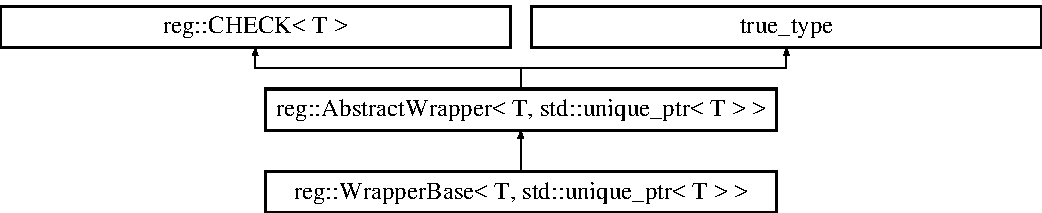
\includegraphics[height=2.866894cm]{structreg_1_1_wrapper_base_3_01_t_00_01std_1_1unique__ptr_3_01_t_01_4_01_4}
\end{center}
\end{figure}
\subsection*{Public Member Functions}
\begin{DoxyCompactItemize}
\item 
T $\ast$ \hyperlink{structreg_1_1_wrapper_base_3_01_t_00_01std_1_1unique__ptr_3_01_t_01_4_01_4_a9f4701d60f0dee6b61ae4046633f3ebe}{Get} () const noexcept override
\item 
void \hyperlink{structreg_1_1_wrapper_base_3_01_t_00_01std_1_1unique__ptr_3_01_t_01_4_01_4_a280dc1e6a85e2a95eaa849a45169942f}{Set} (T $\ast$) noexcept override
\end{DoxyCompactItemize}
\subsection*{Protected Member Functions}
\begin{DoxyCompactItemize}
\item 
void \hyperlink{structreg_1_1_wrapper_base_3_01_t_00_01std_1_1unique__ptr_3_01_t_01_4_01_4_a1b7e67476da7973f319d68e65543d1be}{Allocate} () noexcept override
\end{DoxyCompactItemize}
\subsection*{Additional Inherited Members}


\subsection{Detailed Description}
\subsubsection*{template$<$typename T$>$\newline
struct reg\+::\+Wrapper\+Base$<$ T, std\+::unique\+\_\+ptr$<$ T $>$ $>$}



Definition at line 52 of file Wrapper.\+h.



\subsection{Member Function Documentation}
\mbox{\Hypertarget{structreg_1_1_wrapper_base_3_01_t_00_01std_1_1unique__ptr_3_01_t_01_4_01_4_a1b7e67476da7973f319d68e65543d1be}\label{structreg_1_1_wrapper_base_3_01_t_00_01std_1_1unique__ptr_3_01_t_01_4_01_4_a1b7e67476da7973f319d68e65543d1be}} 
\index{reg\+::\+Wrapper\+Base$<$ T, std\+::unique\+\_\+ptr$<$ T $>$ $>$@{reg\+::\+Wrapper\+Base$<$ T, std\+::unique\+\_\+ptr$<$ T $>$ $>$}!Allocate@{Allocate}}
\index{Allocate@{Allocate}!reg\+::\+Wrapper\+Base$<$ T, std\+::unique\+\_\+ptr$<$ T $>$ $>$@{reg\+::\+Wrapper\+Base$<$ T, std\+::unique\+\_\+ptr$<$ T $>$ $>$}}
\subsubsection{\texorpdfstring{Allocate()}{Allocate()}}
{\footnotesize\ttfamily template$<$typename T $>$ \\
void \hyperlink{structreg_1_1_wrapper_base}{reg\+::\+Wrapper\+Base}$<$ T, std\+::unique\+\_\+ptr$<$ T $>$ $>$\+::Allocate (\begin{DoxyParamCaption}{ }\end{DoxyParamCaption})\hspace{0.3cm}{\ttfamily [inline]}, {\ttfamily [override]}, {\ttfamily [protected]}, {\ttfamily [virtual]}, {\ttfamily [noexcept]}}



Implements \hyperlink{structreg_1_1_abstract_wrapper_aad461ca147a0a7fcfd4f8662994742f3}{reg\+::\+Abstract\+Wrapper$<$ T, std\+::unique\+\_\+ptr$<$ T $>$ $>$}.



Definition at line 182 of file Wrapper.\+h.

\mbox{\Hypertarget{structreg_1_1_wrapper_base_3_01_t_00_01std_1_1unique__ptr_3_01_t_01_4_01_4_a9f4701d60f0dee6b61ae4046633f3ebe}\label{structreg_1_1_wrapper_base_3_01_t_00_01std_1_1unique__ptr_3_01_t_01_4_01_4_a9f4701d60f0dee6b61ae4046633f3ebe}} 
\index{reg\+::\+Wrapper\+Base$<$ T, std\+::unique\+\_\+ptr$<$ T $>$ $>$@{reg\+::\+Wrapper\+Base$<$ T, std\+::unique\+\_\+ptr$<$ T $>$ $>$}!Get@{Get}}
\index{Get@{Get}!reg\+::\+Wrapper\+Base$<$ T, std\+::unique\+\_\+ptr$<$ T $>$ $>$@{reg\+::\+Wrapper\+Base$<$ T, std\+::unique\+\_\+ptr$<$ T $>$ $>$}}
\subsubsection{\texorpdfstring{Get()}{Get()}}
{\footnotesize\ttfamily template$<$typename T $>$ \\
T $\ast$ \hyperlink{structreg_1_1_wrapper_base}{reg\+::\+Wrapper\+Base}$<$ T, std\+::unique\+\_\+ptr$<$ T $>$ $>$\+::Get (\begin{DoxyParamCaption}{ }\end{DoxyParamCaption}) const\hspace{0.3cm}{\ttfamily [inline]}, {\ttfamily [override]}, {\ttfamily [virtual]}, {\ttfamily [noexcept]}}



Implements \hyperlink{structreg_1_1_abstract_wrapper_a88e7079432573b09a5cd695be34e9147}{reg\+::\+Abstract\+Wrapper$<$ T, std\+::unique\+\_\+ptr$<$ T $>$ $>$}.



Definition at line 125 of file Wrapper.\+h.

\mbox{\Hypertarget{structreg_1_1_wrapper_base_3_01_t_00_01std_1_1unique__ptr_3_01_t_01_4_01_4_a280dc1e6a85e2a95eaa849a45169942f}\label{structreg_1_1_wrapper_base_3_01_t_00_01std_1_1unique__ptr_3_01_t_01_4_01_4_a280dc1e6a85e2a95eaa849a45169942f}} 
\index{reg\+::\+Wrapper\+Base$<$ T, std\+::unique\+\_\+ptr$<$ T $>$ $>$@{reg\+::\+Wrapper\+Base$<$ T, std\+::unique\+\_\+ptr$<$ T $>$ $>$}!Set@{Set}}
\index{Set@{Set}!reg\+::\+Wrapper\+Base$<$ T, std\+::unique\+\_\+ptr$<$ T $>$ $>$@{reg\+::\+Wrapper\+Base$<$ T, std\+::unique\+\_\+ptr$<$ T $>$ $>$}}
\subsubsection{\texorpdfstring{Set()}{Set()}}
{\footnotesize\ttfamily template$<$typename T $>$ \\
void \hyperlink{structreg_1_1_wrapper_base}{reg\+::\+Wrapper\+Base}$<$ T, std\+::unique\+\_\+ptr$<$ T $>$ $>$\+::Set (\begin{DoxyParamCaption}\item[{T $\ast$}]{m }\end{DoxyParamCaption})\hspace{0.3cm}{\ttfamily [inline]}, {\ttfamily [override]}, {\ttfamily [virtual]}, {\ttfamily [noexcept]}}



Implements \hyperlink{structreg_1_1_abstract_wrapper_af017f2af039fd5b940345e930e4bb397}{reg\+::\+Abstract\+Wrapper$<$ T, std\+::unique\+\_\+ptr$<$ T $>$ $>$}.



Definition at line 149 of file Wrapper.\+h.



The documentation for this struct was generated from the following file\+:\begin{DoxyCompactItemize}
\item 
/home/adam/\+Desktop/reg/\+Wrapper/\hyperlink{_wrapper_8h}{Wrapper.\+h}\end{DoxyCompactItemize}

\hypertarget{structreg_1_1_wrapper_base_3_01_t_00_01vtk_smart_pointer_3_01_t_01_4_01_4}{}\section{reg\+:\+:Wrapper\+Base$<$ T, vtk\+Smart\+Pointer$<$ T $>$ $>$ Struct Template Reference}
\label{structreg_1_1_wrapper_base_3_01_t_00_01vtk_smart_pointer_3_01_t_01_4_01_4}\index{reg\+::\+Wrapper\+Base$<$ T, vtk\+Smart\+Pointer$<$ T $>$ $>$@{reg\+::\+Wrapper\+Base$<$ T, vtk\+Smart\+Pointer$<$ T $>$ $>$}}


{\ttfamily \#include $<$Wrapper.\+h$>$}

Inheritance diagram for reg\+:\+:Wrapper\+Base$<$ T, vtk\+Smart\+Pointer$<$ T $>$ $>$\+:\begin{figure}[H]
\begin{center}
\leavevmode
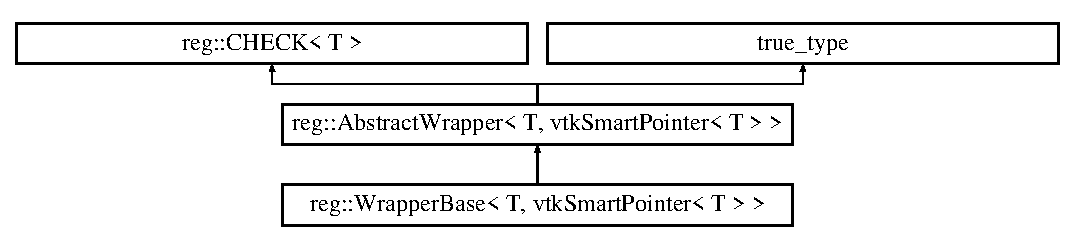
\includegraphics[height=2.800000cm]{structreg_1_1_wrapper_base_3_01_t_00_01vtk_smart_pointer_3_01_t_01_4_01_4}
\end{center}
\end{figure}
\subsection*{Public Member Functions}
\begin{DoxyCompactItemize}
\item 
T $\ast$ \hyperlink{structreg_1_1_wrapper_base_3_01_t_00_01vtk_smart_pointer_3_01_t_01_4_01_4_a61bd745924ef0582ee61ae174ed7479f}{Get} () const noexcept override
\item 
void \hyperlink{structreg_1_1_wrapper_base_3_01_t_00_01vtk_smart_pointer_3_01_t_01_4_01_4_aa066a74ca5abf0e13fd3ed62f0508e32}{Set} (T $\ast$) noexcept override
\end{DoxyCompactItemize}
\subsection*{Protected Member Functions}
\begin{DoxyCompactItemize}
\item 
void \hyperlink{structreg_1_1_wrapper_base_3_01_t_00_01vtk_smart_pointer_3_01_t_01_4_01_4_a3b2609bc1666d9f2dbfe789100889bdc}{Allocate} () noexcept override
\end{DoxyCompactItemize}
\subsection*{Additional Inherited Members}


\subsection{Detailed Description}
\subsubsection*{template$<$typename T$>$\newline
struct reg\+::\+Wrapper\+Base$<$ T, vtk\+Smart\+Pointer$<$ T $>$ $>$}



Definition at line 80 of file Wrapper.\+h.



\subsection{Member Function Documentation}
\mbox{\Hypertarget{structreg_1_1_wrapper_base_3_01_t_00_01vtk_smart_pointer_3_01_t_01_4_01_4_a3b2609bc1666d9f2dbfe789100889bdc}\label{structreg_1_1_wrapper_base_3_01_t_00_01vtk_smart_pointer_3_01_t_01_4_01_4_a3b2609bc1666d9f2dbfe789100889bdc}} 
\index{reg\+::\+Wrapper\+Base$<$ T, vtk\+Smart\+Pointer$<$ T $>$ $>$@{reg\+::\+Wrapper\+Base$<$ T, vtk\+Smart\+Pointer$<$ T $>$ $>$}!Allocate@{Allocate}}
\index{Allocate@{Allocate}!reg\+::\+Wrapper\+Base$<$ T, vtk\+Smart\+Pointer$<$ T $>$ $>$@{reg\+::\+Wrapper\+Base$<$ T, vtk\+Smart\+Pointer$<$ T $>$ $>$}}
\subsubsection{\texorpdfstring{Allocate()}{Allocate()}}
{\footnotesize\ttfamily template$<$typename T $>$ \\
void \hyperlink{structreg_1_1_wrapper_base}{reg\+::\+Wrapper\+Base}$<$ T, vtk\+Smart\+Pointer$<$ T $>$ $>$\+::Allocate (\begin{DoxyParamCaption}{ }\end{DoxyParamCaption})\hspace{0.3cm}{\ttfamily [inline]}, {\ttfamily [override]}, {\ttfamily [protected]}, {\ttfamily [virtual]}, {\ttfamily [noexcept]}}



Implements \hyperlink{structreg_1_1_abstract_wrapper_aad461ca147a0a7fcfd4f8662994742f3}{reg\+::\+Abstract\+Wrapper$<$ T, vtk\+Smart\+Pointer$<$ T $>$ $>$}.



Definition at line 192 of file Wrapper.\+h.

\mbox{\Hypertarget{structreg_1_1_wrapper_base_3_01_t_00_01vtk_smart_pointer_3_01_t_01_4_01_4_a61bd745924ef0582ee61ae174ed7479f}\label{structreg_1_1_wrapper_base_3_01_t_00_01vtk_smart_pointer_3_01_t_01_4_01_4_a61bd745924ef0582ee61ae174ed7479f}} 
\index{reg\+::\+Wrapper\+Base$<$ T, vtk\+Smart\+Pointer$<$ T $>$ $>$@{reg\+::\+Wrapper\+Base$<$ T, vtk\+Smart\+Pointer$<$ T $>$ $>$}!Get@{Get}}
\index{Get@{Get}!reg\+::\+Wrapper\+Base$<$ T, vtk\+Smart\+Pointer$<$ T $>$ $>$@{reg\+::\+Wrapper\+Base$<$ T, vtk\+Smart\+Pointer$<$ T $>$ $>$}}
\subsubsection{\texorpdfstring{Get()}{Get()}}
{\footnotesize\ttfamily template$<$typename T $>$ \\
T $\ast$ \hyperlink{structreg_1_1_wrapper_base}{reg\+::\+Wrapper\+Base}$<$ T, vtk\+Smart\+Pointer$<$ T $>$ $>$\+::Get (\begin{DoxyParamCaption}{ }\end{DoxyParamCaption}) const\hspace{0.3cm}{\ttfamily [inline]}, {\ttfamily [override]}, {\ttfamily [virtual]}, {\ttfamily [noexcept]}}



Implements \hyperlink{structreg_1_1_abstract_wrapper_a88e7079432573b09a5cd695be34e9147}{reg\+::\+Abstract\+Wrapper$<$ T, vtk\+Smart\+Pointer$<$ T $>$ $>$}.



Definition at line 141 of file Wrapper.\+h.

\mbox{\Hypertarget{structreg_1_1_wrapper_base_3_01_t_00_01vtk_smart_pointer_3_01_t_01_4_01_4_aa066a74ca5abf0e13fd3ed62f0508e32}\label{structreg_1_1_wrapper_base_3_01_t_00_01vtk_smart_pointer_3_01_t_01_4_01_4_aa066a74ca5abf0e13fd3ed62f0508e32}} 
\index{reg\+::\+Wrapper\+Base$<$ T, vtk\+Smart\+Pointer$<$ T $>$ $>$@{reg\+::\+Wrapper\+Base$<$ T, vtk\+Smart\+Pointer$<$ T $>$ $>$}!Set@{Set}}
\index{Set@{Set}!reg\+::\+Wrapper\+Base$<$ T, vtk\+Smart\+Pointer$<$ T $>$ $>$@{reg\+::\+Wrapper\+Base$<$ T, vtk\+Smart\+Pointer$<$ T $>$ $>$}}
\subsubsection{\texorpdfstring{Set()}{Set()}}
{\footnotesize\ttfamily template$<$typename T $>$ \\
void \hyperlink{structreg_1_1_wrapper_base}{reg\+::\+Wrapper\+Base}$<$ T, vtk\+Smart\+Pointer$<$ T $>$ $>$\+::Set (\begin{DoxyParamCaption}\item[{T $\ast$}]{m }\end{DoxyParamCaption})\hspace{0.3cm}{\ttfamily [inline]}, {\ttfamily [override]}, {\ttfamily [virtual]}, {\ttfamily [noexcept]}}



Implements \hyperlink{structreg_1_1_abstract_wrapper_af017f2af039fd5b940345e930e4bb397}{reg\+::\+Abstract\+Wrapper$<$ T, vtk\+Smart\+Pointer$<$ T $>$ $>$}.



Definition at line 171 of file Wrapper.\+h.



The documentation for this struct was generated from the following file\+:\begin{DoxyCompactItemize}
\item 
/home/adam/\+Desktop/reg/\+Wrapper/\hyperlink{_wrapper_8h}{Wrapper.\+h}\end{DoxyCompactItemize}

\hypertarget{structreg_1_1_writer}{}\section{reg\+:\+:Writer Struct Reference}
\label{structreg_1_1_writer}\index{reg\+::\+Writer@{reg\+::\+Writer}}


writes itk\+::\+Image$<$double, 3$>$ to given filename  




{\ttfamily \#include $<$Writer.\+h$>$}

Inheritance diagram for reg\+:\+:Writer\+:\begin{figure}[H]
\begin{center}
\leavevmode

\includegraphics[height=0.135331cm]{structreg_1_1_writer}
\end{center}
\end{figure}
\subsection*{Public Member Functions}
\begin{DoxyCompactItemize}
\item 
\hyperlink{structreg_1_1_writer_af4772fac6913708ed8ad4292a908ef7f}{Writer} ()=default
\item 
\hyperlink{structreg_1_1_writer_afbce1fdc6153a79d9affc3c3c0b8b28c}{Writer} (std\+::string \&\&, itk\+::\+Image$<$ double, 3 $>$ $\ast$)
\item 
void \hyperlink{structreg_1_1_writer_abc483635c322211e5e0e8789e4a21a1c}{Execute} (std\+::string \&\&, itk\+::\+Image$<$ double, 3 $>$ $\ast$)
\item 
void \hyperlink{structreg_1_1_writer_af64428b12094aa95d2ee441e6150d409}{Initialize} (std\+::string \&\&, itk\+::\+Image$<$ double, 3 $>$ $\ast$)
\end{DoxyCompactItemize}


\subsection{Detailed Description}
writes itk\+::\+Image$<$double, 3$>$ to given filename 

\begin{DoxyNote}{Note}

\end{DoxyNote}


Definition at line 11 of file Writer.\+h.



\subsection{Constructor \& Destructor Documentation}
\mbox{\Hypertarget{structreg_1_1_writer_af4772fac6913708ed8ad4292a908ef7f}\label{structreg_1_1_writer_af4772fac6913708ed8ad4292a908ef7f}} 
\index{reg\+::\+Writer@{reg\+::\+Writer}!Writer@{Writer}}
\index{Writer@{Writer}!reg\+::\+Writer@{reg\+::\+Writer}}
\subsubsection{\texorpdfstring{Writer()}{Writer()}\hspace{0.1cm}{\footnotesize\ttfamily [1/2]}}
{\footnotesize\ttfamily reg\+::\+Writer\+::\+Writer (\begin{DoxyParamCaption}{ }\end{DoxyParamCaption})\hspace{0.3cm}{\ttfamily [default]}}

\mbox{\Hypertarget{structreg_1_1_writer_afbce1fdc6153a79d9affc3c3c0b8b28c}\label{structreg_1_1_writer_afbce1fdc6153a79d9affc3c3c0b8b28c}} 
\index{reg\+::\+Writer@{reg\+::\+Writer}!Writer@{Writer}}
\index{Writer@{Writer}!reg\+::\+Writer@{reg\+::\+Writer}}
\subsubsection{\texorpdfstring{Writer()}{Writer()}\hspace{0.1cm}{\footnotesize\ttfamily [2/2]}}
{\footnotesize\ttfamily reg\+::\+Writer\+::\+Writer (\begin{DoxyParamCaption}\item[{std\+::string \&\&}]{filename,  }\item[{itk\+::\+Image$<$ double, 3 $>$ $\ast$}]{image }\end{DoxyParamCaption})}



Definition at line 3 of file Writer.\+cpp.



\subsection{Member Function Documentation}
\mbox{\Hypertarget{structreg_1_1_writer_abc483635c322211e5e0e8789e4a21a1c}\label{structreg_1_1_writer_abc483635c322211e5e0e8789e4a21a1c}} 
\index{reg\+::\+Writer@{reg\+::\+Writer}!Execute@{Execute}}
\index{Execute@{Execute}!reg\+::\+Writer@{reg\+::\+Writer}}
\subsubsection{\texorpdfstring{Execute()}{Execute()}}
{\footnotesize\ttfamily void reg\+::\+Writer\+::\+Execute (\begin{DoxyParamCaption}\item[{std\+::string \&\&}]{filename,  }\item[{itk\+::\+Image$<$ double, 3 $>$ $\ast$}]{image }\end{DoxyParamCaption})}



Definition at line 8 of file Writer.\+cpp.

\mbox{\Hypertarget{structreg_1_1_writer_af64428b12094aa95d2ee441e6150d409}\label{structreg_1_1_writer_af64428b12094aa95d2ee441e6150d409}} 
\index{reg\+::\+Writer@{reg\+::\+Writer}!Initialize@{Initialize}}
\index{Initialize@{Initialize}!reg\+::\+Writer@{reg\+::\+Writer}}
\subsubsection{\texorpdfstring{Initialize()}{Initialize()}}
{\footnotesize\ttfamily void reg\+::\+Writer\+::\+Initialize (\begin{DoxyParamCaption}\item[{std\+::string \&\&}]{filename,  }\item[{itk\+::\+Image$<$ double, 3 $>$ $\ast$}]{image }\end{DoxyParamCaption})}



Definition at line 17 of file Writer.\+cpp.



The documentation for this struct was generated from the following files\+:\begin{DoxyCompactItemize}
\item 
/home/adam/\+Desktop/reg/\+Writer/\hyperlink{_writer_8h}{Writer.\+h}\item 
/home/adam/\+Desktop/reg/\+Writer/\hyperlink{_writer_8cpp}{Writer.\+cpp}\end{DoxyCompactItemize}

\chapter{File Documentation}
\hypertarget{build_2_c_make_files_23_87_82_2_compiler_id_c_2_c_make_c_compiler_id_8c}{}\section{/home/adam/\+Desktop/reg/build/\+C\+Make\+Files/3.7.2/\+Compiler\+Id\+C/\+C\+Make\+C\+Compiler\+Id.c File Reference}
\label{build_2_c_make_files_23_87_82_2_compiler_id_c_2_c_make_c_compiler_id_8c}\index{/home/adam/\+Desktop/reg/build/\+C\+Make\+Files/3.\+7.\+2/\+Compiler\+Id\+C/\+C\+Make\+C\+Compiler\+Id.\+c@{/home/adam/\+Desktop/reg/build/\+C\+Make\+Files/3.\+7.\+2/\+Compiler\+Id\+C/\+C\+Make\+C\+Compiler\+Id.\+c}}
\subsection*{Macros}
\begin{DoxyCompactItemize}
\item 
\#define \hyperlink{build_2_c_make_files_23_87_82_2_compiler_id_c_2_c_make_c_compiler_id_8c_a81dee0709ded976b2e0319239f72d174}{C\+O\+M\+P\+I\+L\+E\+R\+\_\+\+ID}~\char`\"{}\char`\"{}
\item 
\#define \hyperlink{build_2_c_make_files_23_87_82_2_compiler_id_c_2_c_make_c_compiler_id_8c_a2ae9b72bb13abaabfcf2ee0ba7d3fa1d}{S\+T\+R\+I\+N\+G\+I\+F\+Y\+\_\+\+H\+E\+L\+P\+ER}(X)~\#X
\item 
\#define \hyperlink{build_2_c_make_files_23_87_82_2_compiler_id_c_2_c_make_c_compiler_id_8c_a43e1cad902b6477bec893cb6430bd6c8}{S\+T\+R\+I\+N\+G\+I\+FY}(X)~\hyperlink{_c_make_files_23_87_82_2_compiler_id_c_x_x_2_c_make_c_x_x_compiler_id_8cpp_a2ae9b72bb13abaabfcf2ee0ba7d3fa1d}{S\+T\+R\+I\+N\+G\+I\+F\+Y\+\_\+\+H\+E\+L\+P\+ER}(X)
\item 
\#define \hyperlink{build_2_c_make_files_23_87_82_2_compiler_id_c_2_c_make_c_compiler_id_8c_adbc5372f40838899018fadbc89bd588b}{P\+L\+A\+T\+F\+O\+R\+M\+\_\+\+ID}
\item 
\#define \hyperlink{build_2_c_make_files_23_87_82_2_compiler_id_c_2_c_make_c_compiler_id_8c_aba35d0d200deaeb06aee95ca297acb28}{A\+R\+C\+H\+I\+T\+E\+C\+T\+U\+R\+E\+\_\+\+ID}
\item 
\#define \hyperlink{build_2_c_make_files_23_87_82_2_compiler_id_c_2_c_make_c_compiler_id_8c_ad1280362da42492bbc11aa78cbf776ad}{D\+EC}(n)
\item 
\#define \hyperlink{build_2_c_make_files_23_87_82_2_compiler_id_c_2_c_make_c_compiler_id_8c_a46d5d95daa1bef867bd0179594310ed5}{H\+EX}(n)
\item 
\#define \hyperlink{build_2_c_make_files_23_87_82_2_compiler_id_c_2_c_make_c_compiler_id_8c_a07f8e5783674099cd7f5110e22a78cdb}{C\+\_\+\+D\+I\+A\+L\+E\+CT}
\end{DoxyCompactItemize}
\subsection*{Functions}
\begin{DoxyCompactItemize}
\item 
int \hyperlink{build_2_c_make_files_23_87_82_2_compiler_id_c_2_c_make_c_compiler_id_8c_a0ddf1224851353fc92bfbff6f499fa97}{main} (int argc, char $\ast$argv\mbox{[}$\,$\mbox{]})
\end{DoxyCompactItemize}
\subsection*{Variables}
\begin{DoxyCompactItemize}
\item 
char const  $\ast$ \hyperlink{build_2_c_make_files_23_87_82_2_compiler_id_c_2_c_make_c_compiler_id_8c_a4b0efeb7a5d59313986b3a0390f050f6}{info\+\_\+compiler} = \char`\"{}I\+N\+FO\char`\"{} \char`\"{}\+:\char`\"{} \char`\"{}compiler\mbox{[}\char`\"{} C\+O\+M\+P\+I\+L\+E\+R\+\_\+\+ID \char`\"{}\mbox{]}\char`\"{}
\item 
char const  $\ast$ \hyperlink{build_2_c_make_files_23_87_82_2_compiler_id_c_2_c_make_c_compiler_id_8c_a2321403dee54ee23f0c2fa849c60f7d4}{info\+\_\+platform} = \char`\"{}I\+N\+FO\char`\"{} \char`\"{}\+:\char`\"{} \char`\"{}platform\mbox{[}\char`\"{} P\+L\+A\+T\+F\+O\+R\+M\+\_\+\+ID \char`\"{}\mbox{]}\char`\"{}
\item 
char const  $\ast$ \hyperlink{build_2_c_make_files_23_87_82_2_compiler_id_c_2_c_make_c_compiler_id_8c_a59647e99d304ed33b15cb284c27ed391}{info\+\_\+arch} = \char`\"{}I\+N\+FO\char`\"{} \char`\"{}\+:\char`\"{} \char`\"{}arch\mbox{[}\char`\"{} A\+R\+C\+H\+I\+T\+E\+C\+T\+U\+R\+E\+\_\+\+ID \char`\"{}\mbox{]}\char`\"{}
\item 
const char $\ast$ \hyperlink{build_2_c_make_files_23_87_82_2_compiler_id_c_2_c_make_c_compiler_id_8c_a1ce162bad2fe6966ac8b33cc19e120b8}{info\+\_\+language\+\_\+dialect\+\_\+default}
\end{DoxyCompactItemize}


\subsection{Macro Definition Documentation}
\mbox{\Hypertarget{build_2_c_make_files_23_87_82_2_compiler_id_c_2_c_make_c_compiler_id_8c_aba35d0d200deaeb06aee95ca297acb28}\label{build_2_c_make_files_23_87_82_2_compiler_id_c_2_c_make_c_compiler_id_8c_aba35d0d200deaeb06aee95ca297acb28}} 
\index{build/\+C\+Make\+Files/3.\+7.\+2/\+Compiler\+Id\+C/\+C\+Make\+C\+Compiler\+Id.\+c@{build/\+C\+Make\+Files/3.\+7.\+2/\+Compiler\+Id\+C/\+C\+Make\+C\+Compiler\+Id.\+c}!A\+R\+C\+H\+I\+T\+E\+C\+T\+U\+R\+E\+\_\+\+ID@{A\+R\+C\+H\+I\+T\+E\+C\+T\+U\+R\+E\+\_\+\+ID}}
\index{A\+R\+C\+H\+I\+T\+E\+C\+T\+U\+R\+E\+\_\+\+ID@{A\+R\+C\+H\+I\+T\+E\+C\+T\+U\+R\+E\+\_\+\+ID}!build/\+C\+Make\+Files/3.\+7.\+2/\+Compiler\+Id\+C/\+C\+Make\+C\+Compiler\+Id.\+c@{build/\+C\+Make\+Files/3.\+7.\+2/\+Compiler\+Id\+C/\+C\+Make\+C\+Compiler\+Id.\+c}}
\subsubsection{\texorpdfstring{A\+R\+C\+H\+I\+T\+E\+C\+T\+U\+R\+E\+\_\+\+ID}{ARCHITECTURE\_ID}}
{\footnotesize\ttfamily \#define A\+R\+C\+H\+I\+T\+E\+C\+T\+U\+R\+E\+\_\+\+ID}



Definition at line 443 of file C\+Make\+C\+Compiler\+Id.\+c.

\mbox{\Hypertarget{build_2_c_make_files_23_87_82_2_compiler_id_c_2_c_make_c_compiler_id_8c_a07f8e5783674099cd7f5110e22a78cdb}\label{build_2_c_make_files_23_87_82_2_compiler_id_c_2_c_make_c_compiler_id_8c_a07f8e5783674099cd7f5110e22a78cdb}} 
\index{build/\+C\+Make\+Files/3.\+7.\+2/\+Compiler\+Id\+C/\+C\+Make\+C\+Compiler\+Id.\+c@{build/\+C\+Make\+Files/3.\+7.\+2/\+Compiler\+Id\+C/\+C\+Make\+C\+Compiler\+Id.\+c}!C\+\_\+\+D\+I\+A\+L\+E\+CT@{C\+\_\+\+D\+I\+A\+L\+E\+CT}}
\index{C\+\_\+\+D\+I\+A\+L\+E\+CT@{C\+\_\+\+D\+I\+A\+L\+E\+CT}!build/\+C\+Make\+Files/3.\+7.\+2/\+Compiler\+Id\+C/\+C\+Make\+C\+Compiler\+Id.\+c@{build/\+C\+Make\+Files/3.\+7.\+2/\+Compiler\+Id\+C/\+C\+Make\+C\+Compiler\+Id.\+c}}
\subsubsection{\texorpdfstring{C\+\_\+\+D\+I\+A\+L\+E\+CT}{C\_DIALECT}}
{\footnotesize\ttfamily \#define C\+\_\+\+D\+I\+A\+L\+E\+CT}



Definition at line 518 of file C\+Make\+C\+Compiler\+Id.\+c.

\mbox{\Hypertarget{build_2_c_make_files_23_87_82_2_compiler_id_c_2_c_make_c_compiler_id_8c_a81dee0709ded976b2e0319239f72d174}\label{build_2_c_make_files_23_87_82_2_compiler_id_c_2_c_make_c_compiler_id_8c_a81dee0709ded976b2e0319239f72d174}} 
\index{build/\+C\+Make\+Files/3.\+7.\+2/\+Compiler\+Id\+C/\+C\+Make\+C\+Compiler\+Id.\+c@{build/\+C\+Make\+Files/3.\+7.\+2/\+Compiler\+Id\+C/\+C\+Make\+C\+Compiler\+Id.\+c}!C\+O\+M\+P\+I\+L\+E\+R\+\_\+\+ID@{C\+O\+M\+P\+I\+L\+E\+R\+\_\+\+ID}}
\index{C\+O\+M\+P\+I\+L\+E\+R\+\_\+\+ID@{C\+O\+M\+P\+I\+L\+E\+R\+\_\+\+ID}!build/\+C\+Make\+Files/3.\+7.\+2/\+Compiler\+Id\+C/\+C\+Make\+C\+Compiler\+Id.\+c@{build/\+C\+Make\+Files/3.\+7.\+2/\+Compiler\+Id\+C/\+C\+Make\+C\+Compiler\+Id.\+c}}
\subsubsection{\texorpdfstring{C\+O\+M\+P\+I\+L\+E\+R\+\_\+\+ID}{COMPILER\_ID}}
{\footnotesize\ttfamily \#define C\+O\+M\+P\+I\+L\+E\+R\+\_\+\+ID~\char`\"{}\char`\"{}}



Definition at line 276 of file C\+Make\+C\+Compiler\+Id.\+c.

\mbox{\Hypertarget{build_2_c_make_files_23_87_82_2_compiler_id_c_2_c_make_c_compiler_id_8c_ad1280362da42492bbc11aa78cbf776ad}\label{build_2_c_make_files_23_87_82_2_compiler_id_c_2_c_make_c_compiler_id_8c_ad1280362da42492bbc11aa78cbf776ad}} 
\index{build/\+C\+Make\+Files/3.\+7.\+2/\+Compiler\+Id\+C/\+C\+Make\+C\+Compiler\+Id.\+c@{build/\+C\+Make\+Files/3.\+7.\+2/\+Compiler\+Id\+C/\+C\+Make\+C\+Compiler\+Id.\+c}!D\+EC@{D\+EC}}
\index{D\+EC@{D\+EC}!build/\+C\+Make\+Files/3.\+7.\+2/\+Compiler\+Id\+C/\+C\+Make\+C\+Compiler\+Id.\+c@{build/\+C\+Make\+Files/3.\+7.\+2/\+Compiler\+Id\+C/\+C\+Make\+C\+Compiler\+Id.\+c}}
\subsubsection{\texorpdfstring{D\+EC}{DEC}}
{\footnotesize\ttfamily \#define D\+EC(\begin{DoxyParamCaption}\item[{}]{n }\end{DoxyParamCaption})}

{\bfseries Value\+:}
\begin{DoxyCode}
(\textcolor{charliteral}{'0'} + (((n) / 10000000)%10)), \(\backslash\)
  (\textcolor{charliteral}{'0'} + (((n) / 1000000)%10)),  \(\backslash\)
  (\textcolor{charliteral}{'0'} + (((n) / 100000)%10)),   \(\backslash\)
  (\textcolor{charliteral}{'0'} + (((n) / 10000)%10)),    \(\backslash\)
  (\textcolor{charliteral}{'0'} + (((n) / 1000)%10)),     \(\backslash\)
  (\textcolor{charliteral}{'0'} + (((n) / 100)%10)),      \(\backslash\)
  (\textcolor{charliteral}{'0'} + (((n) / 10)%10)),       \(\backslash\)
  (\textcolor{charliteral}{'0'} +  ((n) % 10))
\end{DoxyCode}


Definition at line 447 of file C\+Make\+C\+Compiler\+Id.\+c.

\mbox{\Hypertarget{build_2_c_make_files_23_87_82_2_compiler_id_c_2_c_make_c_compiler_id_8c_a46d5d95daa1bef867bd0179594310ed5}\label{build_2_c_make_files_23_87_82_2_compiler_id_c_2_c_make_c_compiler_id_8c_a46d5d95daa1bef867bd0179594310ed5}} 
\index{build/\+C\+Make\+Files/3.\+7.\+2/\+Compiler\+Id\+C/\+C\+Make\+C\+Compiler\+Id.\+c@{build/\+C\+Make\+Files/3.\+7.\+2/\+Compiler\+Id\+C/\+C\+Make\+C\+Compiler\+Id.\+c}!H\+EX@{H\+EX}}
\index{H\+EX@{H\+EX}!build/\+C\+Make\+Files/3.\+7.\+2/\+Compiler\+Id\+C/\+C\+Make\+C\+Compiler\+Id.\+c@{build/\+C\+Make\+Files/3.\+7.\+2/\+Compiler\+Id\+C/\+C\+Make\+C\+Compiler\+Id.\+c}}
\subsubsection{\texorpdfstring{H\+EX}{HEX}}
{\footnotesize\ttfamily \#define H\+EX(\begin{DoxyParamCaption}\item[{}]{n }\end{DoxyParamCaption})}

{\bfseries Value\+:}
\begin{DoxyCode}
(\textcolor{charliteral}{'0'} + ((n)>>28 & 0xF)), \(\backslash\)
  (\textcolor{charliteral}{'0'} + ((n)>>24 & 0xF)), \(\backslash\)
  (\textcolor{charliteral}{'0'} + ((n)>>20 & 0xF)), \(\backslash\)
  (\textcolor{charliteral}{'0'} + ((n)>>16 & 0xF)), \(\backslash\)
  (\textcolor{charliteral}{'0'} + ((n)>>12 & 0xF)), \(\backslash\)
  (\textcolor{charliteral}{'0'} + ((n)>>8  & 0xF)), \(\backslash\)
  (\textcolor{charliteral}{'0'} + ((n)>>4  & 0xF)), \(\backslash\)
  (\textcolor{charliteral}{'0'} + ((n)     & 0xF))
\end{DoxyCode}


Definition at line 458 of file C\+Make\+C\+Compiler\+Id.\+c.

\mbox{\Hypertarget{build_2_c_make_files_23_87_82_2_compiler_id_c_2_c_make_c_compiler_id_8c_adbc5372f40838899018fadbc89bd588b}\label{build_2_c_make_files_23_87_82_2_compiler_id_c_2_c_make_c_compiler_id_8c_adbc5372f40838899018fadbc89bd588b}} 
\index{build/\+C\+Make\+Files/3.\+7.\+2/\+Compiler\+Id\+C/\+C\+Make\+C\+Compiler\+Id.\+c@{build/\+C\+Make\+Files/3.\+7.\+2/\+Compiler\+Id\+C/\+C\+Make\+C\+Compiler\+Id.\+c}!P\+L\+A\+T\+F\+O\+R\+M\+\_\+\+ID@{P\+L\+A\+T\+F\+O\+R\+M\+\_\+\+ID}}
\index{P\+L\+A\+T\+F\+O\+R\+M\+\_\+\+ID@{P\+L\+A\+T\+F\+O\+R\+M\+\_\+\+ID}!build/\+C\+Make\+Files/3.\+7.\+2/\+Compiler\+Id\+C/\+C\+Make\+C\+Compiler\+Id.\+c@{build/\+C\+Make\+Files/3.\+7.\+2/\+Compiler\+Id\+C/\+C\+Make\+C\+Compiler\+Id.\+c}}
\subsubsection{\texorpdfstring{P\+L\+A\+T\+F\+O\+R\+M\+\_\+\+ID}{PLATFORM\_ID}}
{\footnotesize\ttfamily \#define P\+L\+A\+T\+F\+O\+R\+M\+\_\+\+ID}



Definition at line 393 of file C\+Make\+C\+Compiler\+Id.\+c.

\mbox{\Hypertarget{build_2_c_make_files_23_87_82_2_compiler_id_c_2_c_make_c_compiler_id_8c_a43e1cad902b6477bec893cb6430bd6c8}\label{build_2_c_make_files_23_87_82_2_compiler_id_c_2_c_make_c_compiler_id_8c_a43e1cad902b6477bec893cb6430bd6c8}} 
\index{build/\+C\+Make\+Files/3.\+7.\+2/\+Compiler\+Id\+C/\+C\+Make\+C\+Compiler\+Id.\+c@{build/\+C\+Make\+Files/3.\+7.\+2/\+Compiler\+Id\+C/\+C\+Make\+C\+Compiler\+Id.\+c}!S\+T\+R\+I\+N\+G\+I\+FY@{S\+T\+R\+I\+N\+G\+I\+FY}}
\index{S\+T\+R\+I\+N\+G\+I\+FY@{S\+T\+R\+I\+N\+G\+I\+FY}!build/\+C\+Make\+Files/3.\+7.\+2/\+Compiler\+Id\+C/\+C\+Make\+C\+Compiler\+Id.\+c@{build/\+C\+Make\+Files/3.\+7.\+2/\+Compiler\+Id\+C/\+C\+Make\+C\+Compiler\+Id.\+c}}
\subsubsection{\texorpdfstring{S\+T\+R\+I\+N\+G\+I\+FY}{STRINGIFY}}
{\footnotesize\ttfamily \#define S\+T\+R\+I\+N\+G\+I\+FY(\begin{DoxyParamCaption}\item[{}]{X }\end{DoxyParamCaption})~\hyperlink{_c_make_files_23_87_82_2_compiler_id_c_x_x_2_c_make_c_x_x_compiler_id_8cpp_a2ae9b72bb13abaabfcf2ee0ba7d3fa1d}{S\+T\+R\+I\+N\+G\+I\+F\+Y\+\_\+\+H\+E\+L\+P\+ER}(X)}



Definition at line 297 of file C\+Make\+C\+Compiler\+Id.\+c.

\mbox{\Hypertarget{build_2_c_make_files_23_87_82_2_compiler_id_c_2_c_make_c_compiler_id_8c_a2ae9b72bb13abaabfcf2ee0ba7d3fa1d}\label{build_2_c_make_files_23_87_82_2_compiler_id_c_2_c_make_c_compiler_id_8c_a2ae9b72bb13abaabfcf2ee0ba7d3fa1d}} 
\index{build/\+C\+Make\+Files/3.\+7.\+2/\+Compiler\+Id\+C/\+C\+Make\+C\+Compiler\+Id.\+c@{build/\+C\+Make\+Files/3.\+7.\+2/\+Compiler\+Id\+C/\+C\+Make\+C\+Compiler\+Id.\+c}!S\+T\+R\+I\+N\+G\+I\+F\+Y\+\_\+\+H\+E\+L\+P\+ER@{S\+T\+R\+I\+N\+G\+I\+F\+Y\+\_\+\+H\+E\+L\+P\+ER}}
\index{S\+T\+R\+I\+N\+G\+I\+F\+Y\+\_\+\+H\+E\+L\+P\+ER@{S\+T\+R\+I\+N\+G\+I\+F\+Y\+\_\+\+H\+E\+L\+P\+ER}!build/\+C\+Make\+Files/3.\+7.\+2/\+Compiler\+Id\+C/\+C\+Make\+C\+Compiler\+Id.\+c@{build/\+C\+Make\+Files/3.\+7.\+2/\+Compiler\+Id\+C/\+C\+Make\+C\+Compiler\+Id.\+c}}
\subsubsection{\texorpdfstring{S\+T\+R\+I\+N\+G\+I\+F\+Y\+\_\+\+H\+E\+L\+P\+ER}{STRINGIFY\_HELPER}}
{\footnotesize\ttfamily \#define S\+T\+R\+I\+N\+G\+I\+F\+Y\+\_\+\+H\+E\+L\+P\+ER(\begin{DoxyParamCaption}\item[{}]{X }\end{DoxyParamCaption})~\#X}



Definition at line 296 of file C\+Make\+C\+Compiler\+Id.\+c.



\subsection{Function Documentation}
\mbox{\Hypertarget{build_2_c_make_files_23_87_82_2_compiler_id_c_2_c_make_c_compiler_id_8c_a0ddf1224851353fc92bfbff6f499fa97}\label{build_2_c_make_files_23_87_82_2_compiler_id_c_2_c_make_c_compiler_id_8c_a0ddf1224851353fc92bfbff6f499fa97}} 
\index{build/\+C\+Make\+Files/3.\+7.\+2/\+Compiler\+Id\+C/\+C\+Make\+C\+Compiler\+Id.\+c@{build/\+C\+Make\+Files/3.\+7.\+2/\+Compiler\+Id\+C/\+C\+Make\+C\+Compiler\+Id.\+c}!main@{main}}
\index{main@{main}!build/\+C\+Make\+Files/3.\+7.\+2/\+Compiler\+Id\+C/\+C\+Make\+C\+Compiler\+Id.\+c@{build/\+C\+Make\+Files/3.\+7.\+2/\+Compiler\+Id\+C/\+C\+Make\+C\+Compiler\+Id.\+c}}
\subsubsection{\texorpdfstring{main()}{main()}}
{\footnotesize\ttfamily int main (\begin{DoxyParamCaption}\item[{int}]{argc,  }\item[{char $\ast$}]{argv\mbox{[}$\,$\mbox{]} }\end{DoxyParamCaption})}



Definition at line 538 of file C\+Make\+C\+Compiler\+Id.\+c.



\subsection{Variable Documentation}
\mbox{\Hypertarget{build_2_c_make_files_23_87_82_2_compiler_id_c_2_c_make_c_compiler_id_8c_a59647e99d304ed33b15cb284c27ed391}\label{build_2_c_make_files_23_87_82_2_compiler_id_c_2_c_make_c_compiler_id_8c_a59647e99d304ed33b15cb284c27ed391}} 
\index{build/\+C\+Make\+Files/3.\+7.\+2/\+Compiler\+Id\+C/\+C\+Make\+C\+Compiler\+Id.\+c@{build/\+C\+Make\+Files/3.\+7.\+2/\+Compiler\+Id\+C/\+C\+Make\+C\+Compiler\+Id.\+c}!info\+\_\+arch@{info\+\_\+arch}}
\index{info\+\_\+arch@{info\+\_\+arch}!build/\+C\+Make\+Files/3.\+7.\+2/\+Compiler\+Id\+C/\+C\+Make\+C\+Compiler\+Id.\+c@{build/\+C\+Make\+Files/3.\+7.\+2/\+Compiler\+Id\+C/\+C\+Make\+C\+Compiler\+Id.\+c}}
\subsubsection{\texorpdfstring{info\+\_\+arch}{info\_arch}}
{\footnotesize\ttfamily char const$\ast$ info\+\_\+arch = \char`\"{}I\+N\+FO\char`\"{} \char`\"{}\+:\char`\"{} \char`\"{}arch\mbox{[}\char`\"{} A\+R\+C\+H\+I\+T\+E\+C\+T\+U\+R\+E\+\_\+\+ID \char`\"{}\mbox{]}\char`\"{}}



Definition at line 509 of file C\+Make\+C\+Compiler\+Id.\+c.

\mbox{\Hypertarget{build_2_c_make_files_23_87_82_2_compiler_id_c_2_c_make_c_compiler_id_8c_a4b0efeb7a5d59313986b3a0390f050f6}\label{build_2_c_make_files_23_87_82_2_compiler_id_c_2_c_make_c_compiler_id_8c_a4b0efeb7a5d59313986b3a0390f050f6}} 
\index{build/\+C\+Make\+Files/3.\+7.\+2/\+Compiler\+Id\+C/\+C\+Make\+C\+Compiler\+Id.\+c@{build/\+C\+Make\+Files/3.\+7.\+2/\+Compiler\+Id\+C/\+C\+Make\+C\+Compiler\+Id.\+c}!info\+\_\+compiler@{info\+\_\+compiler}}
\index{info\+\_\+compiler@{info\+\_\+compiler}!build/\+C\+Make\+Files/3.\+7.\+2/\+Compiler\+Id\+C/\+C\+Make\+C\+Compiler\+Id.\+c@{build/\+C\+Make\+Files/3.\+7.\+2/\+Compiler\+Id\+C/\+C\+Make\+C\+Compiler\+Id.\+c}}
\subsubsection{\texorpdfstring{info\+\_\+compiler}{info\_compiler}}
{\footnotesize\ttfamily char const$\ast$ info\+\_\+compiler = \char`\"{}I\+N\+FO\char`\"{} \char`\"{}\+:\char`\"{} \char`\"{}compiler\mbox{[}\char`\"{} C\+O\+M\+P\+I\+L\+E\+R\+\_\+\+ID \char`\"{}\mbox{]}\char`\"{}}



Definition at line 283 of file C\+Make\+C\+Compiler\+Id.\+c.

\mbox{\Hypertarget{build_2_c_make_files_23_87_82_2_compiler_id_c_2_c_make_c_compiler_id_8c_a1ce162bad2fe6966ac8b33cc19e120b8}\label{build_2_c_make_files_23_87_82_2_compiler_id_c_2_c_make_c_compiler_id_8c_a1ce162bad2fe6966ac8b33cc19e120b8}} 
\index{build/\+C\+Make\+Files/3.\+7.\+2/\+Compiler\+Id\+C/\+C\+Make\+C\+Compiler\+Id.\+c@{build/\+C\+Make\+Files/3.\+7.\+2/\+Compiler\+Id\+C/\+C\+Make\+C\+Compiler\+Id.\+c}!info\+\_\+language\+\_\+dialect\+\_\+default@{info\+\_\+language\+\_\+dialect\+\_\+default}}
\index{info\+\_\+language\+\_\+dialect\+\_\+default@{info\+\_\+language\+\_\+dialect\+\_\+default}!build/\+C\+Make\+Files/3.\+7.\+2/\+Compiler\+Id\+C/\+C\+Make\+C\+Compiler\+Id.\+c@{build/\+C\+Make\+Files/3.\+7.\+2/\+Compiler\+Id\+C/\+C\+Make\+C\+Compiler\+Id.\+c}}
\subsubsection{\texorpdfstring{info\+\_\+language\+\_\+dialect\+\_\+default}{info\_language\_dialect\_default}}
{\footnotesize\ttfamily const char$\ast$ info\+\_\+language\+\_\+dialect\+\_\+default}

{\bfseries Initial value\+:}
\begin{DoxyCode}
=
  \textcolor{stringliteral}{"INFO"} \textcolor{stringliteral}{":"} \textcolor{stringliteral}{"dialect\_default["} \hyperlink{build_2_c_make_files_23_87_82_2_compiler_id_c_2_c_make_c_compiler_id_8c_a07f8e5783674099cd7f5110e22a78cdb}{C\_DIALECT} \textcolor{stringliteral}{"]"}
\end{DoxyCode}


Definition at line 527 of file C\+Make\+C\+Compiler\+Id.\+c.

\mbox{\Hypertarget{build_2_c_make_files_23_87_82_2_compiler_id_c_2_c_make_c_compiler_id_8c_a2321403dee54ee23f0c2fa849c60f7d4}\label{build_2_c_make_files_23_87_82_2_compiler_id_c_2_c_make_c_compiler_id_8c_a2321403dee54ee23f0c2fa849c60f7d4}} 
\index{build/\+C\+Make\+Files/3.\+7.\+2/\+Compiler\+Id\+C/\+C\+Make\+C\+Compiler\+Id.\+c@{build/\+C\+Make\+Files/3.\+7.\+2/\+Compiler\+Id\+C/\+C\+Make\+C\+Compiler\+Id.\+c}!info\+\_\+platform@{info\+\_\+platform}}
\index{info\+\_\+platform@{info\+\_\+platform}!build/\+C\+Make\+Files/3.\+7.\+2/\+Compiler\+Id\+C/\+C\+Make\+C\+Compiler\+Id.\+c@{build/\+C\+Make\+Files/3.\+7.\+2/\+Compiler\+Id\+C/\+C\+Make\+C\+Compiler\+Id.\+c}}
\subsubsection{\texorpdfstring{info\+\_\+platform}{info\_platform}}
{\footnotesize\ttfamily char const$\ast$ info\+\_\+platform = \char`\"{}I\+N\+FO\char`\"{} \char`\"{}\+:\char`\"{} \char`\"{}platform\mbox{[}\char`\"{} P\+L\+A\+T\+F\+O\+R\+M\+\_\+\+ID \char`\"{}\mbox{]}\char`\"{}}



Definition at line 508 of file C\+Make\+C\+Compiler\+Id.\+c.


\hypertarget{build_2_c_make_files_23_89_81_2_compiler_id_c_2_c_make_c_compiler_id_8c}{}\section{/home/adam/\+Desktop/reg/build/\+C\+Make\+Files/3.9.1/\+Compiler\+Id\+C/\+C\+Make\+C\+Compiler\+Id.c File Reference}
\label{build_2_c_make_files_23_89_81_2_compiler_id_c_2_c_make_c_compiler_id_8c}\index{/home/adam/\+Desktop/reg/build/\+C\+Make\+Files/3.\+9.\+1/\+Compiler\+Id\+C/\+C\+Make\+C\+Compiler\+Id.\+c@{/home/adam/\+Desktop/reg/build/\+C\+Make\+Files/3.\+9.\+1/\+Compiler\+Id\+C/\+C\+Make\+C\+Compiler\+Id.\+c}}
\subsection*{Macros}
\begin{DoxyCompactItemize}
\item 
\#define \hyperlink{build_2_c_make_files_23_89_81_2_compiler_id_c_2_c_make_c_compiler_id_8c_a81dee0709ded976b2e0319239f72d174}{C\+O\+M\+P\+I\+L\+E\+R\+\_\+\+ID}~\char`\"{}\char`\"{}
\item 
\#define \hyperlink{build_2_c_make_files_23_89_81_2_compiler_id_c_2_c_make_c_compiler_id_8c_a2ae9b72bb13abaabfcf2ee0ba7d3fa1d}{S\+T\+R\+I\+N\+G\+I\+F\+Y\+\_\+\+H\+E\+L\+P\+ER}(X)~\#X
\item 
\#define \hyperlink{build_2_c_make_files_23_89_81_2_compiler_id_c_2_c_make_c_compiler_id_8c_a43e1cad902b6477bec893cb6430bd6c8}{S\+T\+R\+I\+N\+G\+I\+FY}(X)~\hyperlink{_c_make_files_23_87_82_2_compiler_id_c_x_x_2_c_make_c_x_x_compiler_id_8cpp_a2ae9b72bb13abaabfcf2ee0ba7d3fa1d}{S\+T\+R\+I\+N\+G\+I\+F\+Y\+\_\+\+H\+E\+L\+P\+ER}(X)
\item 
\#define \hyperlink{build_2_c_make_files_23_89_81_2_compiler_id_c_2_c_make_c_compiler_id_8c_adbc5372f40838899018fadbc89bd588b}{P\+L\+A\+T\+F\+O\+R\+M\+\_\+\+ID}
\item 
\#define \hyperlink{build_2_c_make_files_23_89_81_2_compiler_id_c_2_c_make_c_compiler_id_8c_aba35d0d200deaeb06aee95ca297acb28}{A\+R\+C\+H\+I\+T\+E\+C\+T\+U\+R\+E\+\_\+\+ID}
\item 
\#define \hyperlink{build_2_c_make_files_23_89_81_2_compiler_id_c_2_c_make_c_compiler_id_8c_ad1280362da42492bbc11aa78cbf776ad}{D\+EC}(n)
\item 
\#define \hyperlink{build_2_c_make_files_23_89_81_2_compiler_id_c_2_c_make_c_compiler_id_8c_a46d5d95daa1bef867bd0179594310ed5}{H\+EX}(n)
\item 
\#define \hyperlink{build_2_c_make_files_23_89_81_2_compiler_id_c_2_c_make_c_compiler_id_8c_a07f8e5783674099cd7f5110e22a78cdb}{C\+\_\+\+D\+I\+A\+L\+E\+CT}
\end{DoxyCompactItemize}
\subsection*{Functions}
\begin{DoxyCompactItemize}
\item 
int \hyperlink{build_2_c_make_files_23_89_81_2_compiler_id_c_2_c_make_c_compiler_id_8c_a0ddf1224851353fc92bfbff6f499fa97}{main} (int argc, char $\ast$argv\mbox{[}$\,$\mbox{]})
\end{DoxyCompactItemize}
\subsection*{Variables}
\begin{DoxyCompactItemize}
\item 
char const  $\ast$ \hyperlink{build_2_c_make_files_23_89_81_2_compiler_id_c_2_c_make_c_compiler_id_8c_a4b0efeb7a5d59313986b3a0390f050f6}{info\+\_\+compiler} = \char`\"{}I\+N\+FO\char`\"{} \char`\"{}\+:\char`\"{} \char`\"{}compiler\mbox{[}\char`\"{} C\+O\+M\+P\+I\+L\+E\+R\+\_\+\+ID \char`\"{}\mbox{]}\char`\"{}
\item 
char const  $\ast$ \hyperlink{build_2_c_make_files_23_89_81_2_compiler_id_c_2_c_make_c_compiler_id_8c_a2321403dee54ee23f0c2fa849c60f7d4}{info\+\_\+platform} = \char`\"{}I\+N\+FO\char`\"{} \char`\"{}\+:\char`\"{} \char`\"{}platform\mbox{[}\char`\"{} P\+L\+A\+T\+F\+O\+R\+M\+\_\+\+ID \char`\"{}\mbox{]}\char`\"{}
\item 
char const  $\ast$ \hyperlink{build_2_c_make_files_23_89_81_2_compiler_id_c_2_c_make_c_compiler_id_8c_a59647e99d304ed33b15cb284c27ed391}{info\+\_\+arch} = \char`\"{}I\+N\+FO\char`\"{} \char`\"{}\+:\char`\"{} \char`\"{}arch\mbox{[}\char`\"{} A\+R\+C\+H\+I\+T\+E\+C\+T\+U\+R\+E\+\_\+\+ID \char`\"{}\mbox{]}\char`\"{}
\item 
const char $\ast$ \hyperlink{build_2_c_make_files_23_89_81_2_compiler_id_c_2_c_make_c_compiler_id_8c_a1ce162bad2fe6966ac8b33cc19e120b8}{info\+\_\+language\+\_\+dialect\+\_\+default}
\end{DoxyCompactItemize}


\subsection{Macro Definition Documentation}
\mbox{\Hypertarget{build_2_c_make_files_23_89_81_2_compiler_id_c_2_c_make_c_compiler_id_8c_aba35d0d200deaeb06aee95ca297acb28}\label{build_2_c_make_files_23_89_81_2_compiler_id_c_2_c_make_c_compiler_id_8c_aba35d0d200deaeb06aee95ca297acb28}} 
\index{build/\+C\+Make\+Files/3.\+9.\+1/\+Compiler\+Id\+C/\+C\+Make\+C\+Compiler\+Id.\+c@{build/\+C\+Make\+Files/3.\+9.\+1/\+Compiler\+Id\+C/\+C\+Make\+C\+Compiler\+Id.\+c}!A\+R\+C\+H\+I\+T\+E\+C\+T\+U\+R\+E\+\_\+\+ID@{A\+R\+C\+H\+I\+T\+E\+C\+T\+U\+R\+E\+\_\+\+ID}}
\index{A\+R\+C\+H\+I\+T\+E\+C\+T\+U\+R\+E\+\_\+\+ID@{A\+R\+C\+H\+I\+T\+E\+C\+T\+U\+R\+E\+\_\+\+ID}!build/\+C\+Make\+Files/3.\+9.\+1/\+Compiler\+Id\+C/\+C\+Make\+C\+Compiler\+Id.\+c@{build/\+C\+Make\+Files/3.\+9.\+1/\+Compiler\+Id\+C/\+C\+Make\+C\+Compiler\+Id.\+c}}
\subsubsection{\texorpdfstring{A\+R\+C\+H\+I\+T\+E\+C\+T\+U\+R\+E\+\_\+\+ID}{ARCHITECTURE\_ID}}
{\footnotesize\ttfamily \#define A\+R\+C\+H\+I\+T\+E\+C\+T\+U\+R\+E\+\_\+\+ID}



Definition at line 449 of file C\+Make\+C\+Compiler\+Id.\+c.

\mbox{\Hypertarget{build_2_c_make_files_23_89_81_2_compiler_id_c_2_c_make_c_compiler_id_8c_a07f8e5783674099cd7f5110e22a78cdb}\label{build_2_c_make_files_23_89_81_2_compiler_id_c_2_c_make_c_compiler_id_8c_a07f8e5783674099cd7f5110e22a78cdb}} 
\index{build/\+C\+Make\+Files/3.\+9.\+1/\+Compiler\+Id\+C/\+C\+Make\+C\+Compiler\+Id.\+c@{build/\+C\+Make\+Files/3.\+9.\+1/\+Compiler\+Id\+C/\+C\+Make\+C\+Compiler\+Id.\+c}!C\+\_\+\+D\+I\+A\+L\+E\+CT@{C\+\_\+\+D\+I\+A\+L\+E\+CT}}
\index{C\+\_\+\+D\+I\+A\+L\+E\+CT@{C\+\_\+\+D\+I\+A\+L\+E\+CT}!build/\+C\+Make\+Files/3.\+9.\+1/\+Compiler\+Id\+C/\+C\+Make\+C\+Compiler\+Id.\+c@{build/\+C\+Make\+Files/3.\+9.\+1/\+Compiler\+Id\+C/\+C\+Make\+C\+Compiler\+Id.\+c}}
\subsubsection{\texorpdfstring{C\+\_\+\+D\+I\+A\+L\+E\+CT}{C\_DIALECT}}
{\footnotesize\ttfamily \#define C\+\_\+\+D\+I\+A\+L\+E\+CT}



Definition at line 524 of file C\+Make\+C\+Compiler\+Id.\+c.

\mbox{\Hypertarget{build_2_c_make_files_23_89_81_2_compiler_id_c_2_c_make_c_compiler_id_8c_a81dee0709ded976b2e0319239f72d174}\label{build_2_c_make_files_23_89_81_2_compiler_id_c_2_c_make_c_compiler_id_8c_a81dee0709ded976b2e0319239f72d174}} 
\index{build/\+C\+Make\+Files/3.\+9.\+1/\+Compiler\+Id\+C/\+C\+Make\+C\+Compiler\+Id.\+c@{build/\+C\+Make\+Files/3.\+9.\+1/\+Compiler\+Id\+C/\+C\+Make\+C\+Compiler\+Id.\+c}!C\+O\+M\+P\+I\+L\+E\+R\+\_\+\+ID@{C\+O\+M\+P\+I\+L\+E\+R\+\_\+\+ID}}
\index{C\+O\+M\+P\+I\+L\+E\+R\+\_\+\+ID@{C\+O\+M\+P\+I\+L\+E\+R\+\_\+\+ID}!build/\+C\+Make\+Files/3.\+9.\+1/\+Compiler\+Id\+C/\+C\+Make\+C\+Compiler\+Id.\+c@{build/\+C\+Make\+Files/3.\+9.\+1/\+Compiler\+Id\+C/\+C\+Make\+C\+Compiler\+Id.\+c}}
\subsubsection{\texorpdfstring{C\+O\+M\+P\+I\+L\+E\+R\+\_\+\+ID}{COMPILER\_ID}}
{\footnotesize\ttfamily \#define C\+O\+M\+P\+I\+L\+E\+R\+\_\+\+ID~\char`\"{}\char`\"{}}



Definition at line 282 of file C\+Make\+C\+Compiler\+Id.\+c.

\mbox{\Hypertarget{build_2_c_make_files_23_89_81_2_compiler_id_c_2_c_make_c_compiler_id_8c_ad1280362da42492bbc11aa78cbf776ad}\label{build_2_c_make_files_23_89_81_2_compiler_id_c_2_c_make_c_compiler_id_8c_ad1280362da42492bbc11aa78cbf776ad}} 
\index{build/\+C\+Make\+Files/3.\+9.\+1/\+Compiler\+Id\+C/\+C\+Make\+C\+Compiler\+Id.\+c@{build/\+C\+Make\+Files/3.\+9.\+1/\+Compiler\+Id\+C/\+C\+Make\+C\+Compiler\+Id.\+c}!D\+EC@{D\+EC}}
\index{D\+EC@{D\+EC}!build/\+C\+Make\+Files/3.\+9.\+1/\+Compiler\+Id\+C/\+C\+Make\+C\+Compiler\+Id.\+c@{build/\+C\+Make\+Files/3.\+9.\+1/\+Compiler\+Id\+C/\+C\+Make\+C\+Compiler\+Id.\+c}}
\subsubsection{\texorpdfstring{D\+EC}{DEC}}
{\footnotesize\ttfamily \#define D\+EC(\begin{DoxyParamCaption}\item[{}]{n }\end{DoxyParamCaption})}

{\bfseries Value\+:}
\begin{DoxyCode}
(\textcolor{charliteral}{'0'} + (((n) / 10000000)%10)), \(\backslash\)
  (\textcolor{charliteral}{'0'} + (((n) / 1000000)%10)),  \(\backslash\)
  (\textcolor{charliteral}{'0'} + (((n) / 100000)%10)),   \(\backslash\)
  (\textcolor{charliteral}{'0'} + (((n) / 10000)%10)),    \(\backslash\)
  (\textcolor{charliteral}{'0'} + (((n) / 1000)%10)),     \(\backslash\)
  (\textcolor{charliteral}{'0'} + (((n) / 100)%10)),      \(\backslash\)
  (\textcolor{charliteral}{'0'} + (((n) / 10)%10)),       \(\backslash\)
  (\textcolor{charliteral}{'0'} +  ((n) % 10))
\end{DoxyCode}


Definition at line 453 of file C\+Make\+C\+Compiler\+Id.\+c.

\mbox{\Hypertarget{build_2_c_make_files_23_89_81_2_compiler_id_c_2_c_make_c_compiler_id_8c_a46d5d95daa1bef867bd0179594310ed5}\label{build_2_c_make_files_23_89_81_2_compiler_id_c_2_c_make_c_compiler_id_8c_a46d5d95daa1bef867bd0179594310ed5}} 
\index{build/\+C\+Make\+Files/3.\+9.\+1/\+Compiler\+Id\+C/\+C\+Make\+C\+Compiler\+Id.\+c@{build/\+C\+Make\+Files/3.\+9.\+1/\+Compiler\+Id\+C/\+C\+Make\+C\+Compiler\+Id.\+c}!H\+EX@{H\+EX}}
\index{H\+EX@{H\+EX}!build/\+C\+Make\+Files/3.\+9.\+1/\+Compiler\+Id\+C/\+C\+Make\+C\+Compiler\+Id.\+c@{build/\+C\+Make\+Files/3.\+9.\+1/\+Compiler\+Id\+C/\+C\+Make\+C\+Compiler\+Id.\+c}}
\subsubsection{\texorpdfstring{H\+EX}{HEX}}
{\footnotesize\ttfamily \#define H\+EX(\begin{DoxyParamCaption}\item[{}]{n }\end{DoxyParamCaption})}

{\bfseries Value\+:}
\begin{DoxyCode}
(\textcolor{charliteral}{'0'} + ((n)>>28 & 0xF)), \(\backslash\)
  (\textcolor{charliteral}{'0'} + ((n)>>24 & 0xF)), \(\backslash\)
  (\textcolor{charliteral}{'0'} + ((n)>>20 & 0xF)), \(\backslash\)
  (\textcolor{charliteral}{'0'} + ((n)>>16 & 0xF)), \(\backslash\)
  (\textcolor{charliteral}{'0'} + ((n)>>12 & 0xF)), \(\backslash\)
  (\textcolor{charliteral}{'0'} + ((n)>>8  & 0xF)), \(\backslash\)
  (\textcolor{charliteral}{'0'} + ((n)>>4  & 0xF)), \(\backslash\)
  (\textcolor{charliteral}{'0'} + ((n)     & 0xF))
\end{DoxyCode}


Definition at line 464 of file C\+Make\+C\+Compiler\+Id.\+c.

\mbox{\Hypertarget{build_2_c_make_files_23_89_81_2_compiler_id_c_2_c_make_c_compiler_id_8c_adbc5372f40838899018fadbc89bd588b}\label{build_2_c_make_files_23_89_81_2_compiler_id_c_2_c_make_c_compiler_id_8c_adbc5372f40838899018fadbc89bd588b}} 
\index{build/\+C\+Make\+Files/3.\+9.\+1/\+Compiler\+Id\+C/\+C\+Make\+C\+Compiler\+Id.\+c@{build/\+C\+Make\+Files/3.\+9.\+1/\+Compiler\+Id\+C/\+C\+Make\+C\+Compiler\+Id.\+c}!P\+L\+A\+T\+F\+O\+R\+M\+\_\+\+ID@{P\+L\+A\+T\+F\+O\+R\+M\+\_\+\+ID}}
\index{P\+L\+A\+T\+F\+O\+R\+M\+\_\+\+ID@{P\+L\+A\+T\+F\+O\+R\+M\+\_\+\+ID}!build/\+C\+Make\+Files/3.\+9.\+1/\+Compiler\+Id\+C/\+C\+Make\+C\+Compiler\+Id.\+c@{build/\+C\+Make\+Files/3.\+9.\+1/\+Compiler\+Id\+C/\+C\+Make\+C\+Compiler\+Id.\+c}}
\subsubsection{\texorpdfstring{P\+L\+A\+T\+F\+O\+R\+M\+\_\+\+ID}{PLATFORM\_ID}}
{\footnotesize\ttfamily \#define P\+L\+A\+T\+F\+O\+R\+M\+\_\+\+ID}



Definition at line 399 of file C\+Make\+C\+Compiler\+Id.\+c.

\mbox{\Hypertarget{build_2_c_make_files_23_89_81_2_compiler_id_c_2_c_make_c_compiler_id_8c_a43e1cad902b6477bec893cb6430bd6c8}\label{build_2_c_make_files_23_89_81_2_compiler_id_c_2_c_make_c_compiler_id_8c_a43e1cad902b6477bec893cb6430bd6c8}} 
\index{build/\+C\+Make\+Files/3.\+9.\+1/\+Compiler\+Id\+C/\+C\+Make\+C\+Compiler\+Id.\+c@{build/\+C\+Make\+Files/3.\+9.\+1/\+Compiler\+Id\+C/\+C\+Make\+C\+Compiler\+Id.\+c}!S\+T\+R\+I\+N\+G\+I\+FY@{S\+T\+R\+I\+N\+G\+I\+FY}}
\index{S\+T\+R\+I\+N\+G\+I\+FY@{S\+T\+R\+I\+N\+G\+I\+FY}!build/\+C\+Make\+Files/3.\+9.\+1/\+Compiler\+Id\+C/\+C\+Make\+C\+Compiler\+Id.\+c@{build/\+C\+Make\+Files/3.\+9.\+1/\+Compiler\+Id\+C/\+C\+Make\+C\+Compiler\+Id.\+c}}
\subsubsection{\texorpdfstring{S\+T\+R\+I\+N\+G\+I\+FY}{STRINGIFY}}
{\footnotesize\ttfamily \#define S\+T\+R\+I\+N\+G\+I\+FY(\begin{DoxyParamCaption}\item[{}]{X }\end{DoxyParamCaption})~\hyperlink{_c_make_files_23_87_82_2_compiler_id_c_x_x_2_c_make_c_x_x_compiler_id_8cpp_a2ae9b72bb13abaabfcf2ee0ba7d3fa1d}{S\+T\+R\+I\+N\+G\+I\+F\+Y\+\_\+\+H\+E\+L\+P\+ER}(X)}



Definition at line 303 of file C\+Make\+C\+Compiler\+Id.\+c.

\mbox{\Hypertarget{build_2_c_make_files_23_89_81_2_compiler_id_c_2_c_make_c_compiler_id_8c_a2ae9b72bb13abaabfcf2ee0ba7d3fa1d}\label{build_2_c_make_files_23_89_81_2_compiler_id_c_2_c_make_c_compiler_id_8c_a2ae9b72bb13abaabfcf2ee0ba7d3fa1d}} 
\index{build/\+C\+Make\+Files/3.\+9.\+1/\+Compiler\+Id\+C/\+C\+Make\+C\+Compiler\+Id.\+c@{build/\+C\+Make\+Files/3.\+9.\+1/\+Compiler\+Id\+C/\+C\+Make\+C\+Compiler\+Id.\+c}!S\+T\+R\+I\+N\+G\+I\+F\+Y\+\_\+\+H\+E\+L\+P\+ER@{S\+T\+R\+I\+N\+G\+I\+F\+Y\+\_\+\+H\+E\+L\+P\+ER}}
\index{S\+T\+R\+I\+N\+G\+I\+F\+Y\+\_\+\+H\+E\+L\+P\+ER@{S\+T\+R\+I\+N\+G\+I\+F\+Y\+\_\+\+H\+E\+L\+P\+ER}!build/\+C\+Make\+Files/3.\+9.\+1/\+Compiler\+Id\+C/\+C\+Make\+C\+Compiler\+Id.\+c@{build/\+C\+Make\+Files/3.\+9.\+1/\+Compiler\+Id\+C/\+C\+Make\+C\+Compiler\+Id.\+c}}
\subsubsection{\texorpdfstring{S\+T\+R\+I\+N\+G\+I\+F\+Y\+\_\+\+H\+E\+L\+P\+ER}{STRINGIFY\_HELPER}}
{\footnotesize\ttfamily \#define S\+T\+R\+I\+N\+G\+I\+F\+Y\+\_\+\+H\+E\+L\+P\+ER(\begin{DoxyParamCaption}\item[{}]{X }\end{DoxyParamCaption})~\#X}



Definition at line 302 of file C\+Make\+C\+Compiler\+Id.\+c.



\subsection{Function Documentation}
\mbox{\Hypertarget{build_2_c_make_files_23_89_81_2_compiler_id_c_2_c_make_c_compiler_id_8c_a0ddf1224851353fc92bfbff6f499fa97}\label{build_2_c_make_files_23_89_81_2_compiler_id_c_2_c_make_c_compiler_id_8c_a0ddf1224851353fc92bfbff6f499fa97}} 
\index{build/\+C\+Make\+Files/3.\+9.\+1/\+Compiler\+Id\+C/\+C\+Make\+C\+Compiler\+Id.\+c@{build/\+C\+Make\+Files/3.\+9.\+1/\+Compiler\+Id\+C/\+C\+Make\+C\+Compiler\+Id.\+c}!main@{main}}
\index{main@{main}!build/\+C\+Make\+Files/3.\+9.\+1/\+Compiler\+Id\+C/\+C\+Make\+C\+Compiler\+Id.\+c@{build/\+C\+Make\+Files/3.\+9.\+1/\+Compiler\+Id\+C/\+C\+Make\+C\+Compiler\+Id.\+c}}
\subsubsection{\texorpdfstring{main()}{main()}}
{\footnotesize\ttfamily int main (\begin{DoxyParamCaption}\item[{int}]{argc,  }\item[{char $\ast$}]{argv\mbox{[}$\,$\mbox{]} }\end{DoxyParamCaption})}



Definition at line 544 of file C\+Make\+C\+Compiler\+Id.\+c.



\subsection{Variable Documentation}
\mbox{\Hypertarget{build_2_c_make_files_23_89_81_2_compiler_id_c_2_c_make_c_compiler_id_8c_a59647e99d304ed33b15cb284c27ed391}\label{build_2_c_make_files_23_89_81_2_compiler_id_c_2_c_make_c_compiler_id_8c_a59647e99d304ed33b15cb284c27ed391}} 
\index{build/\+C\+Make\+Files/3.\+9.\+1/\+Compiler\+Id\+C/\+C\+Make\+C\+Compiler\+Id.\+c@{build/\+C\+Make\+Files/3.\+9.\+1/\+Compiler\+Id\+C/\+C\+Make\+C\+Compiler\+Id.\+c}!info\+\_\+arch@{info\+\_\+arch}}
\index{info\+\_\+arch@{info\+\_\+arch}!build/\+C\+Make\+Files/3.\+9.\+1/\+Compiler\+Id\+C/\+C\+Make\+C\+Compiler\+Id.\+c@{build/\+C\+Make\+Files/3.\+9.\+1/\+Compiler\+Id\+C/\+C\+Make\+C\+Compiler\+Id.\+c}}
\subsubsection{\texorpdfstring{info\+\_\+arch}{info\_arch}}
{\footnotesize\ttfamily char const$\ast$ info\+\_\+arch = \char`\"{}I\+N\+FO\char`\"{} \char`\"{}\+:\char`\"{} \char`\"{}arch\mbox{[}\char`\"{} A\+R\+C\+H\+I\+T\+E\+C\+T\+U\+R\+E\+\_\+\+ID \char`\"{}\mbox{]}\char`\"{}}



Definition at line 515 of file C\+Make\+C\+Compiler\+Id.\+c.

\mbox{\Hypertarget{build_2_c_make_files_23_89_81_2_compiler_id_c_2_c_make_c_compiler_id_8c_a4b0efeb7a5d59313986b3a0390f050f6}\label{build_2_c_make_files_23_89_81_2_compiler_id_c_2_c_make_c_compiler_id_8c_a4b0efeb7a5d59313986b3a0390f050f6}} 
\index{build/\+C\+Make\+Files/3.\+9.\+1/\+Compiler\+Id\+C/\+C\+Make\+C\+Compiler\+Id.\+c@{build/\+C\+Make\+Files/3.\+9.\+1/\+Compiler\+Id\+C/\+C\+Make\+C\+Compiler\+Id.\+c}!info\+\_\+compiler@{info\+\_\+compiler}}
\index{info\+\_\+compiler@{info\+\_\+compiler}!build/\+C\+Make\+Files/3.\+9.\+1/\+Compiler\+Id\+C/\+C\+Make\+C\+Compiler\+Id.\+c@{build/\+C\+Make\+Files/3.\+9.\+1/\+Compiler\+Id\+C/\+C\+Make\+C\+Compiler\+Id.\+c}}
\subsubsection{\texorpdfstring{info\+\_\+compiler}{info\_compiler}}
{\footnotesize\ttfamily char const$\ast$ info\+\_\+compiler = \char`\"{}I\+N\+FO\char`\"{} \char`\"{}\+:\char`\"{} \char`\"{}compiler\mbox{[}\char`\"{} C\+O\+M\+P\+I\+L\+E\+R\+\_\+\+ID \char`\"{}\mbox{]}\char`\"{}}



Definition at line 289 of file C\+Make\+C\+Compiler\+Id.\+c.

\mbox{\Hypertarget{build_2_c_make_files_23_89_81_2_compiler_id_c_2_c_make_c_compiler_id_8c_a1ce162bad2fe6966ac8b33cc19e120b8}\label{build_2_c_make_files_23_89_81_2_compiler_id_c_2_c_make_c_compiler_id_8c_a1ce162bad2fe6966ac8b33cc19e120b8}} 
\index{build/\+C\+Make\+Files/3.\+9.\+1/\+Compiler\+Id\+C/\+C\+Make\+C\+Compiler\+Id.\+c@{build/\+C\+Make\+Files/3.\+9.\+1/\+Compiler\+Id\+C/\+C\+Make\+C\+Compiler\+Id.\+c}!info\+\_\+language\+\_\+dialect\+\_\+default@{info\+\_\+language\+\_\+dialect\+\_\+default}}
\index{info\+\_\+language\+\_\+dialect\+\_\+default@{info\+\_\+language\+\_\+dialect\+\_\+default}!build/\+C\+Make\+Files/3.\+9.\+1/\+Compiler\+Id\+C/\+C\+Make\+C\+Compiler\+Id.\+c@{build/\+C\+Make\+Files/3.\+9.\+1/\+Compiler\+Id\+C/\+C\+Make\+C\+Compiler\+Id.\+c}}
\subsubsection{\texorpdfstring{info\+\_\+language\+\_\+dialect\+\_\+default}{info\_language\_dialect\_default}}
{\footnotesize\ttfamily const char$\ast$ info\+\_\+language\+\_\+dialect\+\_\+default}

{\bfseries Initial value\+:}
\begin{DoxyCode}
=
  \textcolor{stringliteral}{"INFO"} \textcolor{stringliteral}{":"} \textcolor{stringliteral}{"dialect\_default["} \hyperlink{build_2_c_make_files_23_89_81_2_compiler_id_c_2_c_make_c_compiler_id_8c_a07f8e5783674099cd7f5110e22a78cdb}{C\_DIALECT} \textcolor{stringliteral}{"]"}
\end{DoxyCode}


Definition at line 533 of file C\+Make\+C\+Compiler\+Id.\+c.

\mbox{\Hypertarget{build_2_c_make_files_23_89_81_2_compiler_id_c_2_c_make_c_compiler_id_8c_a2321403dee54ee23f0c2fa849c60f7d4}\label{build_2_c_make_files_23_89_81_2_compiler_id_c_2_c_make_c_compiler_id_8c_a2321403dee54ee23f0c2fa849c60f7d4}} 
\index{build/\+C\+Make\+Files/3.\+9.\+1/\+Compiler\+Id\+C/\+C\+Make\+C\+Compiler\+Id.\+c@{build/\+C\+Make\+Files/3.\+9.\+1/\+Compiler\+Id\+C/\+C\+Make\+C\+Compiler\+Id.\+c}!info\+\_\+platform@{info\+\_\+platform}}
\index{info\+\_\+platform@{info\+\_\+platform}!build/\+C\+Make\+Files/3.\+9.\+1/\+Compiler\+Id\+C/\+C\+Make\+C\+Compiler\+Id.\+c@{build/\+C\+Make\+Files/3.\+9.\+1/\+Compiler\+Id\+C/\+C\+Make\+C\+Compiler\+Id.\+c}}
\subsubsection{\texorpdfstring{info\+\_\+platform}{info\_platform}}
{\footnotesize\ttfamily char const$\ast$ info\+\_\+platform = \char`\"{}I\+N\+FO\char`\"{} \char`\"{}\+:\char`\"{} \char`\"{}platform\mbox{[}\char`\"{} P\+L\+A\+T\+F\+O\+R\+M\+\_\+\+ID \char`\"{}\mbox{]}\char`\"{}}



Definition at line 514 of file C\+Make\+C\+Compiler\+Id.\+c.


\hypertarget{_c_make_files_23_87_82_2_compiler_id_c_2_c_make_c_compiler_id_8c}{}\section{/home/adam/\+Desktop/reg/\+C\+Make\+Files/3.7.2/\+Compiler\+Id\+C/\+C\+Make\+C\+Compiler\+Id.c File Reference}
\label{_c_make_files_23_87_82_2_compiler_id_c_2_c_make_c_compiler_id_8c}\index{/home/adam/\+Desktop/reg/\+C\+Make\+Files/3.\+7.\+2/\+Compiler\+Id\+C/\+C\+Make\+C\+Compiler\+Id.\+c@{/home/adam/\+Desktop/reg/\+C\+Make\+Files/3.\+7.\+2/\+Compiler\+Id\+C/\+C\+Make\+C\+Compiler\+Id.\+c}}
\subsection*{Macros}
\begin{DoxyCompactItemize}
\item 
\#define \hyperlink{_c_make_files_23_87_82_2_compiler_id_c_2_c_make_c_compiler_id_8c_a81dee0709ded976b2e0319239f72d174}{C\+O\+M\+P\+I\+L\+E\+R\+\_\+\+ID}~\char`\"{}\char`\"{}
\item 
\#define \hyperlink{_c_make_files_23_87_82_2_compiler_id_c_2_c_make_c_compiler_id_8c_a2ae9b72bb13abaabfcf2ee0ba7d3fa1d}{S\+T\+R\+I\+N\+G\+I\+F\+Y\+\_\+\+H\+E\+L\+P\+ER}(X)~\#X
\item 
\#define \hyperlink{_c_make_files_23_87_82_2_compiler_id_c_2_c_make_c_compiler_id_8c_a43e1cad902b6477bec893cb6430bd6c8}{S\+T\+R\+I\+N\+G\+I\+FY}(X)~\hyperlink{_c_make_files_23_87_82_2_compiler_id_c_x_x_2_c_make_c_x_x_compiler_id_8cpp_a2ae9b72bb13abaabfcf2ee0ba7d3fa1d}{S\+T\+R\+I\+N\+G\+I\+F\+Y\+\_\+\+H\+E\+L\+P\+ER}(X)
\item 
\#define \hyperlink{_c_make_files_23_87_82_2_compiler_id_c_2_c_make_c_compiler_id_8c_adbc5372f40838899018fadbc89bd588b}{P\+L\+A\+T\+F\+O\+R\+M\+\_\+\+ID}
\item 
\#define \hyperlink{_c_make_files_23_87_82_2_compiler_id_c_2_c_make_c_compiler_id_8c_aba35d0d200deaeb06aee95ca297acb28}{A\+R\+C\+H\+I\+T\+E\+C\+T\+U\+R\+E\+\_\+\+ID}
\item 
\#define \hyperlink{_c_make_files_23_87_82_2_compiler_id_c_2_c_make_c_compiler_id_8c_ad1280362da42492bbc11aa78cbf776ad}{D\+EC}(n)
\item 
\#define \hyperlink{_c_make_files_23_87_82_2_compiler_id_c_2_c_make_c_compiler_id_8c_a46d5d95daa1bef867bd0179594310ed5}{H\+EX}(n)
\item 
\#define \hyperlink{_c_make_files_23_87_82_2_compiler_id_c_2_c_make_c_compiler_id_8c_a07f8e5783674099cd7f5110e22a78cdb}{C\+\_\+\+D\+I\+A\+L\+E\+CT}
\end{DoxyCompactItemize}
\subsection*{Functions}
\begin{DoxyCompactItemize}
\item 
int \hyperlink{_c_make_files_23_87_82_2_compiler_id_c_2_c_make_c_compiler_id_8c_a0ddf1224851353fc92bfbff6f499fa97}{main} (int argc, char $\ast$argv\mbox{[}$\,$\mbox{]})
\end{DoxyCompactItemize}
\subsection*{Variables}
\begin{DoxyCompactItemize}
\item 
char const  $\ast$ \hyperlink{_c_make_files_23_87_82_2_compiler_id_c_2_c_make_c_compiler_id_8c_a4b0efeb7a5d59313986b3a0390f050f6}{info\+\_\+compiler} = \char`\"{}I\+N\+FO\char`\"{} \char`\"{}\+:\char`\"{} \char`\"{}compiler\mbox{[}\char`\"{} C\+O\+M\+P\+I\+L\+E\+R\+\_\+\+ID \char`\"{}\mbox{]}\char`\"{}
\item 
char const  $\ast$ \hyperlink{_c_make_files_23_87_82_2_compiler_id_c_2_c_make_c_compiler_id_8c_a2321403dee54ee23f0c2fa849c60f7d4}{info\+\_\+platform} = \char`\"{}I\+N\+FO\char`\"{} \char`\"{}\+:\char`\"{} \char`\"{}platform\mbox{[}\char`\"{} P\+L\+A\+T\+F\+O\+R\+M\+\_\+\+ID \char`\"{}\mbox{]}\char`\"{}
\item 
char const  $\ast$ \hyperlink{_c_make_files_23_87_82_2_compiler_id_c_2_c_make_c_compiler_id_8c_a59647e99d304ed33b15cb284c27ed391}{info\+\_\+arch} = \char`\"{}I\+N\+FO\char`\"{} \char`\"{}\+:\char`\"{} \char`\"{}arch\mbox{[}\char`\"{} A\+R\+C\+H\+I\+T\+E\+C\+T\+U\+R\+E\+\_\+\+ID \char`\"{}\mbox{]}\char`\"{}
\item 
const char $\ast$ \hyperlink{_c_make_files_23_87_82_2_compiler_id_c_2_c_make_c_compiler_id_8c_a1ce162bad2fe6966ac8b33cc19e120b8}{info\+\_\+language\+\_\+dialect\+\_\+default}
\end{DoxyCompactItemize}


\subsection{Macro Definition Documentation}
\mbox{\Hypertarget{_c_make_files_23_87_82_2_compiler_id_c_2_c_make_c_compiler_id_8c_aba35d0d200deaeb06aee95ca297acb28}\label{_c_make_files_23_87_82_2_compiler_id_c_2_c_make_c_compiler_id_8c_aba35d0d200deaeb06aee95ca297acb28}} 
\index{C\+Make\+Files/3.\+7.\+2/\+Compiler\+Id\+C/\+C\+Make\+C\+Compiler\+Id.\+c@{C\+Make\+Files/3.\+7.\+2/\+Compiler\+Id\+C/\+C\+Make\+C\+Compiler\+Id.\+c}!A\+R\+C\+H\+I\+T\+E\+C\+T\+U\+R\+E\+\_\+\+ID@{A\+R\+C\+H\+I\+T\+E\+C\+T\+U\+R\+E\+\_\+\+ID}}
\index{A\+R\+C\+H\+I\+T\+E\+C\+T\+U\+R\+E\+\_\+\+ID@{A\+R\+C\+H\+I\+T\+E\+C\+T\+U\+R\+E\+\_\+\+ID}!C\+Make\+Files/3.\+7.\+2/\+Compiler\+Id\+C/\+C\+Make\+C\+Compiler\+Id.\+c@{C\+Make\+Files/3.\+7.\+2/\+Compiler\+Id\+C/\+C\+Make\+C\+Compiler\+Id.\+c}}
\subsubsection{\texorpdfstring{A\+R\+C\+H\+I\+T\+E\+C\+T\+U\+R\+E\+\_\+\+ID}{ARCHITECTURE\_ID}}
{\footnotesize\ttfamily \#define A\+R\+C\+H\+I\+T\+E\+C\+T\+U\+R\+E\+\_\+\+ID}



Definition at line 443 of file C\+Make\+C\+Compiler\+Id.\+c.

\mbox{\Hypertarget{_c_make_files_23_87_82_2_compiler_id_c_2_c_make_c_compiler_id_8c_a07f8e5783674099cd7f5110e22a78cdb}\label{_c_make_files_23_87_82_2_compiler_id_c_2_c_make_c_compiler_id_8c_a07f8e5783674099cd7f5110e22a78cdb}} 
\index{C\+Make\+Files/3.\+7.\+2/\+Compiler\+Id\+C/\+C\+Make\+C\+Compiler\+Id.\+c@{C\+Make\+Files/3.\+7.\+2/\+Compiler\+Id\+C/\+C\+Make\+C\+Compiler\+Id.\+c}!C\+\_\+\+D\+I\+A\+L\+E\+CT@{C\+\_\+\+D\+I\+A\+L\+E\+CT}}
\index{C\+\_\+\+D\+I\+A\+L\+E\+CT@{C\+\_\+\+D\+I\+A\+L\+E\+CT}!C\+Make\+Files/3.\+7.\+2/\+Compiler\+Id\+C/\+C\+Make\+C\+Compiler\+Id.\+c@{C\+Make\+Files/3.\+7.\+2/\+Compiler\+Id\+C/\+C\+Make\+C\+Compiler\+Id.\+c}}
\subsubsection{\texorpdfstring{C\+\_\+\+D\+I\+A\+L\+E\+CT}{C\_DIALECT}}
{\footnotesize\ttfamily \#define C\+\_\+\+D\+I\+A\+L\+E\+CT}



Definition at line 518 of file C\+Make\+C\+Compiler\+Id.\+c.

\mbox{\Hypertarget{_c_make_files_23_87_82_2_compiler_id_c_2_c_make_c_compiler_id_8c_a81dee0709ded976b2e0319239f72d174}\label{_c_make_files_23_87_82_2_compiler_id_c_2_c_make_c_compiler_id_8c_a81dee0709ded976b2e0319239f72d174}} 
\index{C\+Make\+Files/3.\+7.\+2/\+Compiler\+Id\+C/\+C\+Make\+C\+Compiler\+Id.\+c@{C\+Make\+Files/3.\+7.\+2/\+Compiler\+Id\+C/\+C\+Make\+C\+Compiler\+Id.\+c}!C\+O\+M\+P\+I\+L\+E\+R\+\_\+\+ID@{C\+O\+M\+P\+I\+L\+E\+R\+\_\+\+ID}}
\index{C\+O\+M\+P\+I\+L\+E\+R\+\_\+\+ID@{C\+O\+M\+P\+I\+L\+E\+R\+\_\+\+ID}!C\+Make\+Files/3.\+7.\+2/\+Compiler\+Id\+C/\+C\+Make\+C\+Compiler\+Id.\+c@{C\+Make\+Files/3.\+7.\+2/\+Compiler\+Id\+C/\+C\+Make\+C\+Compiler\+Id.\+c}}
\subsubsection{\texorpdfstring{C\+O\+M\+P\+I\+L\+E\+R\+\_\+\+ID}{COMPILER\_ID}}
{\footnotesize\ttfamily \#define C\+O\+M\+P\+I\+L\+E\+R\+\_\+\+ID~\char`\"{}\char`\"{}}



Definition at line 276 of file C\+Make\+C\+Compiler\+Id.\+c.

\mbox{\Hypertarget{_c_make_files_23_87_82_2_compiler_id_c_2_c_make_c_compiler_id_8c_ad1280362da42492bbc11aa78cbf776ad}\label{_c_make_files_23_87_82_2_compiler_id_c_2_c_make_c_compiler_id_8c_ad1280362da42492bbc11aa78cbf776ad}} 
\index{C\+Make\+Files/3.\+7.\+2/\+Compiler\+Id\+C/\+C\+Make\+C\+Compiler\+Id.\+c@{C\+Make\+Files/3.\+7.\+2/\+Compiler\+Id\+C/\+C\+Make\+C\+Compiler\+Id.\+c}!D\+EC@{D\+EC}}
\index{D\+EC@{D\+EC}!C\+Make\+Files/3.\+7.\+2/\+Compiler\+Id\+C/\+C\+Make\+C\+Compiler\+Id.\+c@{C\+Make\+Files/3.\+7.\+2/\+Compiler\+Id\+C/\+C\+Make\+C\+Compiler\+Id.\+c}}
\subsubsection{\texorpdfstring{D\+EC}{DEC}}
{\footnotesize\ttfamily \#define D\+EC(\begin{DoxyParamCaption}\item[{}]{n }\end{DoxyParamCaption})}

{\bfseries Value\+:}
\begin{DoxyCode}
(\textcolor{charliteral}{'0'} + (((n) / 10000000)%10)), \(\backslash\)
  (\textcolor{charliteral}{'0'} + (((n) / 1000000)%10)),  \(\backslash\)
  (\textcolor{charliteral}{'0'} + (((n) / 100000)%10)),   \(\backslash\)
  (\textcolor{charliteral}{'0'} + (((n) / 10000)%10)),    \(\backslash\)
  (\textcolor{charliteral}{'0'} + (((n) / 1000)%10)),     \(\backslash\)
  (\textcolor{charliteral}{'0'} + (((n) / 100)%10)),      \(\backslash\)
  (\textcolor{charliteral}{'0'} + (((n) / 10)%10)),       \(\backslash\)
  (\textcolor{charliteral}{'0'} +  ((n) % 10))
\end{DoxyCode}


Definition at line 447 of file C\+Make\+C\+Compiler\+Id.\+c.

\mbox{\Hypertarget{_c_make_files_23_87_82_2_compiler_id_c_2_c_make_c_compiler_id_8c_a46d5d95daa1bef867bd0179594310ed5}\label{_c_make_files_23_87_82_2_compiler_id_c_2_c_make_c_compiler_id_8c_a46d5d95daa1bef867bd0179594310ed5}} 
\index{C\+Make\+Files/3.\+7.\+2/\+Compiler\+Id\+C/\+C\+Make\+C\+Compiler\+Id.\+c@{C\+Make\+Files/3.\+7.\+2/\+Compiler\+Id\+C/\+C\+Make\+C\+Compiler\+Id.\+c}!H\+EX@{H\+EX}}
\index{H\+EX@{H\+EX}!C\+Make\+Files/3.\+7.\+2/\+Compiler\+Id\+C/\+C\+Make\+C\+Compiler\+Id.\+c@{C\+Make\+Files/3.\+7.\+2/\+Compiler\+Id\+C/\+C\+Make\+C\+Compiler\+Id.\+c}}
\subsubsection{\texorpdfstring{H\+EX}{HEX}}
{\footnotesize\ttfamily \#define H\+EX(\begin{DoxyParamCaption}\item[{}]{n }\end{DoxyParamCaption})}

{\bfseries Value\+:}
\begin{DoxyCode}
(\textcolor{charliteral}{'0'} + ((n)>>28 & 0xF)), \(\backslash\)
  (\textcolor{charliteral}{'0'} + ((n)>>24 & 0xF)), \(\backslash\)
  (\textcolor{charliteral}{'0'} + ((n)>>20 & 0xF)), \(\backslash\)
  (\textcolor{charliteral}{'0'} + ((n)>>16 & 0xF)), \(\backslash\)
  (\textcolor{charliteral}{'0'} + ((n)>>12 & 0xF)), \(\backslash\)
  (\textcolor{charliteral}{'0'} + ((n)>>8  & 0xF)), \(\backslash\)
  (\textcolor{charliteral}{'0'} + ((n)>>4  & 0xF)), \(\backslash\)
  (\textcolor{charliteral}{'0'} + ((n)     & 0xF))
\end{DoxyCode}


Definition at line 458 of file C\+Make\+C\+Compiler\+Id.\+c.

\mbox{\Hypertarget{_c_make_files_23_87_82_2_compiler_id_c_2_c_make_c_compiler_id_8c_adbc5372f40838899018fadbc89bd588b}\label{_c_make_files_23_87_82_2_compiler_id_c_2_c_make_c_compiler_id_8c_adbc5372f40838899018fadbc89bd588b}} 
\index{C\+Make\+Files/3.\+7.\+2/\+Compiler\+Id\+C/\+C\+Make\+C\+Compiler\+Id.\+c@{C\+Make\+Files/3.\+7.\+2/\+Compiler\+Id\+C/\+C\+Make\+C\+Compiler\+Id.\+c}!P\+L\+A\+T\+F\+O\+R\+M\+\_\+\+ID@{P\+L\+A\+T\+F\+O\+R\+M\+\_\+\+ID}}
\index{P\+L\+A\+T\+F\+O\+R\+M\+\_\+\+ID@{P\+L\+A\+T\+F\+O\+R\+M\+\_\+\+ID}!C\+Make\+Files/3.\+7.\+2/\+Compiler\+Id\+C/\+C\+Make\+C\+Compiler\+Id.\+c@{C\+Make\+Files/3.\+7.\+2/\+Compiler\+Id\+C/\+C\+Make\+C\+Compiler\+Id.\+c}}
\subsubsection{\texorpdfstring{P\+L\+A\+T\+F\+O\+R\+M\+\_\+\+ID}{PLATFORM\_ID}}
{\footnotesize\ttfamily \#define P\+L\+A\+T\+F\+O\+R\+M\+\_\+\+ID}



Definition at line 393 of file C\+Make\+C\+Compiler\+Id.\+c.

\mbox{\Hypertarget{_c_make_files_23_87_82_2_compiler_id_c_2_c_make_c_compiler_id_8c_a43e1cad902b6477bec893cb6430bd6c8}\label{_c_make_files_23_87_82_2_compiler_id_c_2_c_make_c_compiler_id_8c_a43e1cad902b6477bec893cb6430bd6c8}} 
\index{C\+Make\+Files/3.\+7.\+2/\+Compiler\+Id\+C/\+C\+Make\+C\+Compiler\+Id.\+c@{C\+Make\+Files/3.\+7.\+2/\+Compiler\+Id\+C/\+C\+Make\+C\+Compiler\+Id.\+c}!S\+T\+R\+I\+N\+G\+I\+FY@{S\+T\+R\+I\+N\+G\+I\+FY}}
\index{S\+T\+R\+I\+N\+G\+I\+FY@{S\+T\+R\+I\+N\+G\+I\+FY}!C\+Make\+Files/3.\+7.\+2/\+Compiler\+Id\+C/\+C\+Make\+C\+Compiler\+Id.\+c@{C\+Make\+Files/3.\+7.\+2/\+Compiler\+Id\+C/\+C\+Make\+C\+Compiler\+Id.\+c}}
\subsubsection{\texorpdfstring{S\+T\+R\+I\+N\+G\+I\+FY}{STRINGIFY}}
{\footnotesize\ttfamily \#define S\+T\+R\+I\+N\+G\+I\+FY(\begin{DoxyParamCaption}\item[{}]{X }\end{DoxyParamCaption})~\hyperlink{_c_make_files_23_87_82_2_compiler_id_c_x_x_2_c_make_c_x_x_compiler_id_8cpp_a2ae9b72bb13abaabfcf2ee0ba7d3fa1d}{S\+T\+R\+I\+N\+G\+I\+F\+Y\+\_\+\+H\+E\+L\+P\+ER}(X)}



Definition at line 297 of file C\+Make\+C\+Compiler\+Id.\+c.

\mbox{\Hypertarget{_c_make_files_23_87_82_2_compiler_id_c_2_c_make_c_compiler_id_8c_a2ae9b72bb13abaabfcf2ee0ba7d3fa1d}\label{_c_make_files_23_87_82_2_compiler_id_c_2_c_make_c_compiler_id_8c_a2ae9b72bb13abaabfcf2ee0ba7d3fa1d}} 
\index{C\+Make\+Files/3.\+7.\+2/\+Compiler\+Id\+C/\+C\+Make\+C\+Compiler\+Id.\+c@{C\+Make\+Files/3.\+7.\+2/\+Compiler\+Id\+C/\+C\+Make\+C\+Compiler\+Id.\+c}!S\+T\+R\+I\+N\+G\+I\+F\+Y\+\_\+\+H\+E\+L\+P\+ER@{S\+T\+R\+I\+N\+G\+I\+F\+Y\+\_\+\+H\+E\+L\+P\+ER}}
\index{S\+T\+R\+I\+N\+G\+I\+F\+Y\+\_\+\+H\+E\+L\+P\+ER@{S\+T\+R\+I\+N\+G\+I\+F\+Y\+\_\+\+H\+E\+L\+P\+ER}!C\+Make\+Files/3.\+7.\+2/\+Compiler\+Id\+C/\+C\+Make\+C\+Compiler\+Id.\+c@{C\+Make\+Files/3.\+7.\+2/\+Compiler\+Id\+C/\+C\+Make\+C\+Compiler\+Id.\+c}}
\subsubsection{\texorpdfstring{S\+T\+R\+I\+N\+G\+I\+F\+Y\+\_\+\+H\+E\+L\+P\+ER}{STRINGIFY\_HELPER}}
{\footnotesize\ttfamily \#define S\+T\+R\+I\+N\+G\+I\+F\+Y\+\_\+\+H\+E\+L\+P\+ER(\begin{DoxyParamCaption}\item[{}]{X }\end{DoxyParamCaption})~\#X}



Definition at line 296 of file C\+Make\+C\+Compiler\+Id.\+c.



\subsection{Function Documentation}
\mbox{\Hypertarget{_c_make_files_23_87_82_2_compiler_id_c_2_c_make_c_compiler_id_8c_a0ddf1224851353fc92bfbff6f499fa97}\label{_c_make_files_23_87_82_2_compiler_id_c_2_c_make_c_compiler_id_8c_a0ddf1224851353fc92bfbff6f499fa97}} 
\index{C\+Make\+Files/3.\+7.\+2/\+Compiler\+Id\+C/\+C\+Make\+C\+Compiler\+Id.\+c@{C\+Make\+Files/3.\+7.\+2/\+Compiler\+Id\+C/\+C\+Make\+C\+Compiler\+Id.\+c}!main@{main}}
\index{main@{main}!C\+Make\+Files/3.\+7.\+2/\+Compiler\+Id\+C/\+C\+Make\+C\+Compiler\+Id.\+c@{C\+Make\+Files/3.\+7.\+2/\+Compiler\+Id\+C/\+C\+Make\+C\+Compiler\+Id.\+c}}
\subsubsection{\texorpdfstring{main()}{main()}}
{\footnotesize\ttfamily int main (\begin{DoxyParamCaption}\item[{int}]{argc,  }\item[{char $\ast$}]{argv\mbox{[}$\,$\mbox{]} }\end{DoxyParamCaption})}



Definition at line 538 of file C\+Make\+C\+Compiler\+Id.\+c.



\subsection{Variable Documentation}
\mbox{\Hypertarget{_c_make_files_23_87_82_2_compiler_id_c_2_c_make_c_compiler_id_8c_a59647e99d304ed33b15cb284c27ed391}\label{_c_make_files_23_87_82_2_compiler_id_c_2_c_make_c_compiler_id_8c_a59647e99d304ed33b15cb284c27ed391}} 
\index{C\+Make\+Files/3.\+7.\+2/\+Compiler\+Id\+C/\+C\+Make\+C\+Compiler\+Id.\+c@{C\+Make\+Files/3.\+7.\+2/\+Compiler\+Id\+C/\+C\+Make\+C\+Compiler\+Id.\+c}!info\+\_\+arch@{info\+\_\+arch}}
\index{info\+\_\+arch@{info\+\_\+arch}!C\+Make\+Files/3.\+7.\+2/\+Compiler\+Id\+C/\+C\+Make\+C\+Compiler\+Id.\+c@{C\+Make\+Files/3.\+7.\+2/\+Compiler\+Id\+C/\+C\+Make\+C\+Compiler\+Id.\+c}}
\subsubsection{\texorpdfstring{info\+\_\+arch}{info\_arch}}
{\footnotesize\ttfamily char const$\ast$ info\+\_\+arch = \char`\"{}I\+N\+FO\char`\"{} \char`\"{}\+:\char`\"{} \char`\"{}arch\mbox{[}\char`\"{} A\+R\+C\+H\+I\+T\+E\+C\+T\+U\+R\+E\+\_\+\+ID \char`\"{}\mbox{]}\char`\"{}}



Definition at line 509 of file C\+Make\+C\+Compiler\+Id.\+c.

\mbox{\Hypertarget{_c_make_files_23_87_82_2_compiler_id_c_2_c_make_c_compiler_id_8c_a4b0efeb7a5d59313986b3a0390f050f6}\label{_c_make_files_23_87_82_2_compiler_id_c_2_c_make_c_compiler_id_8c_a4b0efeb7a5d59313986b3a0390f050f6}} 
\index{C\+Make\+Files/3.\+7.\+2/\+Compiler\+Id\+C/\+C\+Make\+C\+Compiler\+Id.\+c@{C\+Make\+Files/3.\+7.\+2/\+Compiler\+Id\+C/\+C\+Make\+C\+Compiler\+Id.\+c}!info\+\_\+compiler@{info\+\_\+compiler}}
\index{info\+\_\+compiler@{info\+\_\+compiler}!C\+Make\+Files/3.\+7.\+2/\+Compiler\+Id\+C/\+C\+Make\+C\+Compiler\+Id.\+c@{C\+Make\+Files/3.\+7.\+2/\+Compiler\+Id\+C/\+C\+Make\+C\+Compiler\+Id.\+c}}
\subsubsection{\texorpdfstring{info\+\_\+compiler}{info\_compiler}}
{\footnotesize\ttfamily char const$\ast$ info\+\_\+compiler = \char`\"{}I\+N\+FO\char`\"{} \char`\"{}\+:\char`\"{} \char`\"{}compiler\mbox{[}\char`\"{} C\+O\+M\+P\+I\+L\+E\+R\+\_\+\+ID \char`\"{}\mbox{]}\char`\"{}}



Definition at line 283 of file C\+Make\+C\+Compiler\+Id.\+c.

\mbox{\Hypertarget{_c_make_files_23_87_82_2_compiler_id_c_2_c_make_c_compiler_id_8c_a1ce162bad2fe6966ac8b33cc19e120b8}\label{_c_make_files_23_87_82_2_compiler_id_c_2_c_make_c_compiler_id_8c_a1ce162bad2fe6966ac8b33cc19e120b8}} 
\index{C\+Make\+Files/3.\+7.\+2/\+Compiler\+Id\+C/\+C\+Make\+C\+Compiler\+Id.\+c@{C\+Make\+Files/3.\+7.\+2/\+Compiler\+Id\+C/\+C\+Make\+C\+Compiler\+Id.\+c}!info\+\_\+language\+\_\+dialect\+\_\+default@{info\+\_\+language\+\_\+dialect\+\_\+default}}
\index{info\+\_\+language\+\_\+dialect\+\_\+default@{info\+\_\+language\+\_\+dialect\+\_\+default}!C\+Make\+Files/3.\+7.\+2/\+Compiler\+Id\+C/\+C\+Make\+C\+Compiler\+Id.\+c@{C\+Make\+Files/3.\+7.\+2/\+Compiler\+Id\+C/\+C\+Make\+C\+Compiler\+Id.\+c}}
\subsubsection{\texorpdfstring{info\+\_\+language\+\_\+dialect\+\_\+default}{info\_language\_dialect\_default}}
{\footnotesize\ttfamily const char$\ast$ info\+\_\+language\+\_\+dialect\+\_\+default}

{\bfseries Initial value\+:}
\begin{DoxyCode}
=
  \textcolor{stringliteral}{"INFO"} \textcolor{stringliteral}{":"} \textcolor{stringliteral}{"dialect\_default["} \hyperlink{_c_make_files_23_87_82_2_compiler_id_c_2_c_make_c_compiler_id_8c_a07f8e5783674099cd7f5110e22a78cdb}{C\_DIALECT} \textcolor{stringliteral}{"]"}
\end{DoxyCode}


Definition at line 527 of file C\+Make\+C\+Compiler\+Id.\+c.

\mbox{\Hypertarget{_c_make_files_23_87_82_2_compiler_id_c_2_c_make_c_compiler_id_8c_a2321403dee54ee23f0c2fa849c60f7d4}\label{_c_make_files_23_87_82_2_compiler_id_c_2_c_make_c_compiler_id_8c_a2321403dee54ee23f0c2fa849c60f7d4}} 
\index{C\+Make\+Files/3.\+7.\+2/\+Compiler\+Id\+C/\+C\+Make\+C\+Compiler\+Id.\+c@{C\+Make\+Files/3.\+7.\+2/\+Compiler\+Id\+C/\+C\+Make\+C\+Compiler\+Id.\+c}!info\+\_\+platform@{info\+\_\+platform}}
\index{info\+\_\+platform@{info\+\_\+platform}!C\+Make\+Files/3.\+7.\+2/\+Compiler\+Id\+C/\+C\+Make\+C\+Compiler\+Id.\+c@{C\+Make\+Files/3.\+7.\+2/\+Compiler\+Id\+C/\+C\+Make\+C\+Compiler\+Id.\+c}}
\subsubsection{\texorpdfstring{info\+\_\+platform}{info\_platform}}
{\footnotesize\ttfamily char const$\ast$ info\+\_\+platform = \char`\"{}I\+N\+FO\char`\"{} \char`\"{}\+:\char`\"{} \char`\"{}platform\mbox{[}\char`\"{} P\+L\+A\+T\+F\+O\+R\+M\+\_\+\+ID \char`\"{}\mbox{]}\char`\"{}}



Definition at line 508 of file C\+Make\+C\+Compiler\+Id.\+c.


\hypertarget{build_2_c_make_files_23_87_82_2_compiler_id_c_x_x_2_c_make_c_x_x_compiler_id_8cpp}{}\section{/home/adam/\+Desktop/reg/build/\+C\+Make\+Files/3.7.2/\+Compiler\+Id\+C\+X\+X/\+C\+Make\+C\+X\+X\+Compiler\+Id.cpp File Reference}
\label{build_2_c_make_files_23_87_82_2_compiler_id_c_x_x_2_c_make_c_x_x_compiler_id_8cpp}\index{/home/adam/\+Desktop/reg/build/\+C\+Make\+Files/3.\+7.\+2/\+Compiler\+Id\+C\+X\+X/\+C\+Make\+C\+X\+X\+Compiler\+Id.\+cpp@{/home/adam/\+Desktop/reg/build/\+C\+Make\+Files/3.\+7.\+2/\+Compiler\+Id\+C\+X\+X/\+C\+Make\+C\+X\+X\+Compiler\+Id.\+cpp}}
\subsection*{Macros}
\begin{DoxyCompactItemize}
\item 
\#define \hyperlink{build_2_c_make_files_23_87_82_2_compiler_id_c_x_x_2_c_make_c_x_x_compiler_id_8cpp_a81dee0709ded976b2e0319239f72d174}{C\+O\+M\+P\+I\+L\+E\+R\+\_\+\+ID}~\char`\"{}\char`\"{}
\item 
\#define \hyperlink{build_2_c_make_files_23_87_82_2_compiler_id_c_x_x_2_c_make_c_x_x_compiler_id_8cpp_a2ae9b72bb13abaabfcf2ee0ba7d3fa1d}{S\+T\+R\+I\+N\+G\+I\+F\+Y\+\_\+\+H\+E\+L\+P\+ER}(X)~\#X
\item 
\#define \hyperlink{build_2_c_make_files_23_87_82_2_compiler_id_c_x_x_2_c_make_c_x_x_compiler_id_8cpp_a43e1cad902b6477bec893cb6430bd6c8}{S\+T\+R\+I\+N\+G\+I\+FY}(X)~\hyperlink{_c_make_files_23_87_82_2_compiler_id_c_x_x_2_c_make_c_x_x_compiler_id_8cpp_a2ae9b72bb13abaabfcf2ee0ba7d3fa1d}{S\+T\+R\+I\+N\+G\+I\+F\+Y\+\_\+\+H\+E\+L\+P\+ER}(X)
\item 
\#define \hyperlink{build_2_c_make_files_23_87_82_2_compiler_id_c_x_x_2_c_make_c_x_x_compiler_id_8cpp_adbc5372f40838899018fadbc89bd588b}{P\+L\+A\+T\+F\+O\+R\+M\+\_\+\+ID}
\item 
\#define \hyperlink{build_2_c_make_files_23_87_82_2_compiler_id_c_x_x_2_c_make_c_x_x_compiler_id_8cpp_aba35d0d200deaeb06aee95ca297acb28}{A\+R\+C\+H\+I\+T\+E\+C\+T\+U\+R\+E\+\_\+\+ID}
\item 
\#define \hyperlink{build_2_c_make_files_23_87_82_2_compiler_id_c_x_x_2_c_make_c_x_x_compiler_id_8cpp_ad1280362da42492bbc11aa78cbf776ad}{D\+EC}(n)
\item 
\#define \hyperlink{build_2_c_make_files_23_87_82_2_compiler_id_c_x_x_2_c_make_c_x_x_compiler_id_8cpp_a46d5d95daa1bef867bd0179594310ed5}{H\+EX}(n)
\end{DoxyCompactItemize}
\subsection*{Functions}
\begin{DoxyCompactItemize}
\item 
int \hyperlink{build_2_c_make_files_23_87_82_2_compiler_id_c_x_x_2_c_make_c_x_x_compiler_id_8cpp_a0ddf1224851353fc92bfbff6f499fa97}{main} (int argc, char $\ast$argv\mbox{[}$\,$\mbox{]})
\end{DoxyCompactItemize}
\subsection*{Variables}
\begin{DoxyCompactItemize}
\item 
char const  $\ast$ \hyperlink{build_2_c_make_files_23_87_82_2_compiler_id_c_x_x_2_c_make_c_x_x_compiler_id_8cpp_a4b0efeb7a5d59313986b3a0390f050f6}{info\+\_\+compiler} = \char`\"{}I\+N\+FO\char`\"{} \char`\"{}\+:\char`\"{} \char`\"{}compiler\mbox{[}\char`\"{} C\+O\+M\+P\+I\+L\+E\+R\+\_\+\+ID \char`\"{}\mbox{]}\char`\"{}
\item 
char const  $\ast$ \hyperlink{build_2_c_make_files_23_87_82_2_compiler_id_c_x_x_2_c_make_c_x_x_compiler_id_8cpp_a2321403dee54ee23f0c2fa849c60f7d4}{info\+\_\+platform} = \char`\"{}I\+N\+FO\char`\"{} \char`\"{}\+:\char`\"{} \char`\"{}platform\mbox{[}\char`\"{} P\+L\+A\+T\+F\+O\+R\+M\+\_\+\+ID \char`\"{}\mbox{]}\char`\"{}
\item 
char const  $\ast$ \hyperlink{build_2_c_make_files_23_87_82_2_compiler_id_c_x_x_2_c_make_c_x_x_compiler_id_8cpp_a59647e99d304ed33b15cb284c27ed391}{info\+\_\+arch} = \char`\"{}I\+N\+FO\char`\"{} \char`\"{}\+:\char`\"{} \char`\"{}arch\mbox{[}\char`\"{} A\+R\+C\+H\+I\+T\+E\+C\+T\+U\+R\+E\+\_\+\+ID \char`\"{}\mbox{]}\char`\"{}
\item 
const char $\ast$ \hyperlink{build_2_c_make_files_23_87_82_2_compiler_id_c_x_x_2_c_make_c_x_x_compiler_id_8cpp_a1ce162bad2fe6966ac8b33cc19e120b8}{info\+\_\+language\+\_\+dialect\+\_\+default}
\end{DoxyCompactItemize}


\subsection{Macro Definition Documentation}
\mbox{\Hypertarget{build_2_c_make_files_23_87_82_2_compiler_id_c_x_x_2_c_make_c_x_x_compiler_id_8cpp_aba35d0d200deaeb06aee95ca297acb28}\label{build_2_c_make_files_23_87_82_2_compiler_id_c_x_x_2_c_make_c_x_x_compiler_id_8cpp_aba35d0d200deaeb06aee95ca297acb28}} 
\index{build/\+C\+Make\+Files/3.\+7.\+2/\+Compiler\+Id\+C\+X\+X/\+C\+Make\+C\+X\+X\+Compiler\+Id.\+cpp@{build/\+C\+Make\+Files/3.\+7.\+2/\+Compiler\+Id\+C\+X\+X/\+C\+Make\+C\+X\+X\+Compiler\+Id.\+cpp}!A\+R\+C\+H\+I\+T\+E\+C\+T\+U\+R\+E\+\_\+\+ID@{A\+R\+C\+H\+I\+T\+E\+C\+T\+U\+R\+E\+\_\+\+ID}}
\index{A\+R\+C\+H\+I\+T\+E\+C\+T\+U\+R\+E\+\_\+\+ID@{A\+R\+C\+H\+I\+T\+E\+C\+T\+U\+R\+E\+\_\+\+ID}!build/\+C\+Make\+Files/3.\+7.\+2/\+Compiler\+Id\+C\+X\+X/\+C\+Make\+C\+X\+X\+Compiler\+Id.\+cpp@{build/\+C\+Make\+Files/3.\+7.\+2/\+Compiler\+Id\+C\+X\+X/\+C\+Make\+C\+X\+X\+Compiler\+Id.\+cpp}}
\subsubsection{\texorpdfstring{A\+R\+C\+H\+I\+T\+E\+C\+T\+U\+R\+E\+\_\+\+ID}{ARCHITECTURE\_ID}}
{\footnotesize\ttfamily \#define A\+R\+C\+H\+I\+T\+E\+C\+T\+U\+R\+E\+\_\+\+ID}



Definition at line 430 of file C\+Make\+C\+X\+X\+Compiler\+Id.\+cpp.

\mbox{\Hypertarget{build_2_c_make_files_23_87_82_2_compiler_id_c_x_x_2_c_make_c_x_x_compiler_id_8cpp_a81dee0709ded976b2e0319239f72d174}\label{build_2_c_make_files_23_87_82_2_compiler_id_c_x_x_2_c_make_c_x_x_compiler_id_8cpp_a81dee0709ded976b2e0319239f72d174}} 
\index{build/\+C\+Make\+Files/3.\+7.\+2/\+Compiler\+Id\+C\+X\+X/\+C\+Make\+C\+X\+X\+Compiler\+Id.\+cpp@{build/\+C\+Make\+Files/3.\+7.\+2/\+Compiler\+Id\+C\+X\+X/\+C\+Make\+C\+X\+X\+Compiler\+Id.\+cpp}!C\+O\+M\+P\+I\+L\+E\+R\+\_\+\+ID@{C\+O\+M\+P\+I\+L\+E\+R\+\_\+\+ID}}
\index{C\+O\+M\+P\+I\+L\+E\+R\+\_\+\+ID@{C\+O\+M\+P\+I\+L\+E\+R\+\_\+\+ID}!build/\+C\+Make\+Files/3.\+7.\+2/\+Compiler\+Id\+C\+X\+X/\+C\+Make\+C\+X\+X\+Compiler\+Id.\+cpp@{build/\+C\+Make\+Files/3.\+7.\+2/\+Compiler\+Id\+C\+X\+X/\+C\+Make\+C\+X\+X\+Compiler\+Id.\+cpp}}
\subsubsection{\texorpdfstring{C\+O\+M\+P\+I\+L\+E\+R\+\_\+\+ID}{COMPILER\_ID}}
{\footnotesize\ttfamily \#define C\+O\+M\+P\+I\+L\+E\+R\+\_\+\+ID~\char`\"{}\char`\"{}}



Definition at line 263 of file C\+Make\+C\+X\+X\+Compiler\+Id.\+cpp.

\mbox{\Hypertarget{build_2_c_make_files_23_87_82_2_compiler_id_c_x_x_2_c_make_c_x_x_compiler_id_8cpp_ad1280362da42492bbc11aa78cbf776ad}\label{build_2_c_make_files_23_87_82_2_compiler_id_c_x_x_2_c_make_c_x_x_compiler_id_8cpp_ad1280362da42492bbc11aa78cbf776ad}} 
\index{build/\+C\+Make\+Files/3.\+7.\+2/\+Compiler\+Id\+C\+X\+X/\+C\+Make\+C\+X\+X\+Compiler\+Id.\+cpp@{build/\+C\+Make\+Files/3.\+7.\+2/\+Compiler\+Id\+C\+X\+X/\+C\+Make\+C\+X\+X\+Compiler\+Id.\+cpp}!D\+EC@{D\+EC}}
\index{D\+EC@{D\+EC}!build/\+C\+Make\+Files/3.\+7.\+2/\+Compiler\+Id\+C\+X\+X/\+C\+Make\+C\+X\+X\+Compiler\+Id.\+cpp@{build/\+C\+Make\+Files/3.\+7.\+2/\+Compiler\+Id\+C\+X\+X/\+C\+Make\+C\+X\+X\+Compiler\+Id.\+cpp}}
\subsubsection{\texorpdfstring{D\+EC}{DEC}}
{\footnotesize\ttfamily \#define D\+EC(\begin{DoxyParamCaption}\item[{}]{n }\end{DoxyParamCaption})}

{\bfseries Value\+:}
\begin{DoxyCode}
(\textcolor{charliteral}{'0'} + (((n) / 10000000)%10)), \(\backslash\)
  (\textcolor{charliteral}{'0'} + (((n) / 1000000)%10)),  \(\backslash\)
  (\textcolor{charliteral}{'0'} + (((n) / 100000)%10)),   \(\backslash\)
  (\textcolor{charliteral}{'0'} + (((n) / 10000)%10)),    \(\backslash\)
  (\textcolor{charliteral}{'0'} + (((n) / 1000)%10)),     \(\backslash\)
  (\textcolor{charliteral}{'0'} + (((n) / 100)%10)),      \(\backslash\)
  (\textcolor{charliteral}{'0'} + (((n) / 10)%10)),       \(\backslash\)
  (\textcolor{charliteral}{'0'} +  ((n) % 10))
\end{DoxyCode}


Definition at line 434 of file C\+Make\+C\+X\+X\+Compiler\+Id.\+cpp.

\mbox{\Hypertarget{build_2_c_make_files_23_87_82_2_compiler_id_c_x_x_2_c_make_c_x_x_compiler_id_8cpp_a46d5d95daa1bef867bd0179594310ed5}\label{build_2_c_make_files_23_87_82_2_compiler_id_c_x_x_2_c_make_c_x_x_compiler_id_8cpp_a46d5d95daa1bef867bd0179594310ed5}} 
\index{build/\+C\+Make\+Files/3.\+7.\+2/\+Compiler\+Id\+C\+X\+X/\+C\+Make\+C\+X\+X\+Compiler\+Id.\+cpp@{build/\+C\+Make\+Files/3.\+7.\+2/\+Compiler\+Id\+C\+X\+X/\+C\+Make\+C\+X\+X\+Compiler\+Id.\+cpp}!H\+EX@{H\+EX}}
\index{H\+EX@{H\+EX}!build/\+C\+Make\+Files/3.\+7.\+2/\+Compiler\+Id\+C\+X\+X/\+C\+Make\+C\+X\+X\+Compiler\+Id.\+cpp@{build/\+C\+Make\+Files/3.\+7.\+2/\+Compiler\+Id\+C\+X\+X/\+C\+Make\+C\+X\+X\+Compiler\+Id.\+cpp}}
\subsubsection{\texorpdfstring{H\+EX}{HEX}}
{\footnotesize\ttfamily \#define H\+EX(\begin{DoxyParamCaption}\item[{}]{n }\end{DoxyParamCaption})}

{\bfseries Value\+:}
\begin{DoxyCode}
(\textcolor{charliteral}{'0'} + ((n)>>28 & 0xF)), \(\backslash\)
  (\textcolor{charliteral}{'0'} + ((n)>>24 & 0xF)), \(\backslash\)
  (\textcolor{charliteral}{'0'} + ((n)>>20 & 0xF)), \(\backslash\)
  (\textcolor{charliteral}{'0'} + ((n)>>16 & 0xF)), \(\backslash\)
  (\textcolor{charliteral}{'0'} + ((n)>>12 & 0xF)), \(\backslash\)
  (\textcolor{charliteral}{'0'} + ((n)>>8  & 0xF)), \(\backslash\)
  (\textcolor{charliteral}{'0'} + ((n)>>4  & 0xF)), \(\backslash\)
  (\textcolor{charliteral}{'0'} + ((n)     & 0xF))
\end{DoxyCode}


Definition at line 445 of file C\+Make\+C\+X\+X\+Compiler\+Id.\+cpp.

\mbox{\Hypertarget{build_2_c_make_files_23_87_82_2_compiler_id_c_x_x_2_c_make_c_x_x_compiler_id_8cpp_adbc5372f40838899018fadbc89bd588b}\label{build_2_c_make_files_23_87_82_2_compiler_id_c_x_x_2_c_make_c_x_x_compiler_id_8cpp_adbc5372f40838899018fadbc89bd588b}} 
\index{build/\+C\+Make\+Files/3.\+7.\+2/\+Compiler\+Id\+C\+X\+X/\+C\+Make\+C\+X\+X\+Compiler\+Id.\+cpp@{build/\+C\+Make\+Files/3.\+7.\+2/\+Compiler\+Id\+C\+X\+X/\+C\+Make\+C\+X\+X\+Compiler\+Id.\+cpp}!P\+L\+A\+T\+F\+O\+R\+M\+\_\+\+ID@{P\+L\+A\+T\+F\+O\+R\+M\+\_\+\+ID}}
\index{P\+L\+A\+T\+F\+O\+R\+M\+\_\+\+ID@{P\+L\+A\+T\+F\+O\+R\+M\+\_\+\+ID}!build/\+C\+Make\+Files/3.\+7.\+2/\+Compiler\+Id\+C\+X\+X/\+C\+Make\+C\+X\+X\+Compiler\+Id.\+cpp@{build/\+C\+Make\+Files/3.\+7.\+2/\+Compiler\+Id\+C\+X\+X/\+C\+Make\+C\+X\+X\+Compiler\+Id.\+cpp}}
\subsubsection{\texorpdfstring{P\+L\+A\+T\+F\+O\+R\+M\+\_\+\+ID}{PLATFORM\_ID}}
{\footnotesize\ttfamily \#define P\+L\+A\+T\+F\+O\+R\+M\+\_\+\+ID}



Definition at line 380 of file C\+Make\+C\+X\+X\+Compiler\+Id.\+cpp.

\mbox{\Hypertarget{build_2_c_make_files_23_87_82_2_compiler_id_c_x_x_2_c_make_c_x_x_compiler_id_8cpp_a43e1cad902b6477bec893cb6430bd6c8}\label{build_2_c_make_files_23_87_82_2_compiler_id_c_x_x_2_c_make_c_x_x_compiler_id_8cpp_a43e1cad902b6477bec893cb6430bd6c8}} 
\index{build/\+C\+Make\+Files/3.\+7.\+2/\+Compiler\+Id\+C\+X\+X/\+C\+Make\+C\+X\+X\+Compiler\+Id.\+cpp@{build/\+C\+Make\+Files/3.\+7.\+2/\+Compiler\+Id\+C\+X\+X/\+C\+Make\+C\+X\+X\+Compiler\+Id.\+cpp}!S\+T\+R\+I\+N\+G\+I\+FY@{S\+T\+R\+I\+N\+G\+I\+FY}}
\index{S\+T\+R\+I\+N\+G\+I\+FY@{S\+T\+R\+I\+N\+G\+I\+FY}!build/\+C\+Make\+Files/3.\+7.\+2/\+Compiler\+Id\+C\+X\+X/\+C\+Make\+C\+X\+X\+Compiler\+Id.\+cpp@{build/\+C\+Make\+Files/3.\+7.\+2/\+Compiler\+Id\+C\+X\+X/\+C\+Make\+C\+X\+X\+Compiler\+Id.\+cpp}}
\subsubsection{\texorpdfstring{S\+T\+R\+I\+N\+G\+I\+FY}{STRINGIFY}}
{\footnotesize\ttfamily \#define S\+T\+R\+I\+N\+G\+I\+FY(\begin{DoxyParamCaption}\item[{}]{X }\end{DoxyParamCaption})~\hyperlink{_c_make_files_23_87_82_2_compiler_id_c_x_x_2_c_make_c_x_x_compiler_id_8cpp_a2ae9b72bb13abaabfcf2ee0ba7d3fa1d}{S\+T\+R\+I\+N\+G\+I\+F\+Y\+\_\+\+H\+E\+L\+P\+ER}(X)}



Definition at line 284 of file C\+Make\+C\+X\+X\+Compiler\+Id.\+cpp.

\mbox{\Hypertarget{build_2_c_make_files_23_87_82_2_compiler_id_c_x_x_2_c_make_c_x_x_compiler_id_8cpp_a2ae9b72bb13abaabfcf2ee0ba7d3fa1d}\label{build_2_c_make_files_23_87_82_2_compiler_id_c_x_x_2_c_make_c_x_x_compiler_id_8cpp_a2ae9b72bb13abaabfcf2ee0ba7d3fa1d}} 
\index{build/\+C\+Make\+Files/3.\+7.\+2/\+Compiler\+Id\+C\+X\+X/\+C\+Make\+C\+X\+X\+Compiler\+Id.\+cpp@{build/\+C\+Make\+Files/3.\+7.\+2/\+Compiler\+Id\+C\+X\+X/\+C\+Make\+C\+X\+X\+Compiler\+Id.\+cpp}!S\+T\+R\+I\+N\+G\+I\+F\+Y\+\_\+\+H\+E\+L\+P\+ER@{S\+T\+R\+I\+N\+G\+I\+F\+Y\+\_\+\+H\+E\+L\+P\+ER}}
\index{S\+T\+R\+I\+N\+G\+I\+F\+Y\+\_\+\+H\+E\+L\+P\+ER@{S\+T\+R\+I\+N\+G\+I\+F\+Y\+\_\+\+H\+E\+L\+P\+ER}!build/\+C\+Make\+Files/3.\+7.\+2/\+Compiler\+Id\+C\+X\+X/\+C\+Make\+C\+X\+X\+Compiler\+Id.\+cpp@{build/\+C\+Make\+Files/3.\+7.\+2/\+Compiler\+Id\+C\+X\+X/\+C\+Make\+C\+X\+X\+Compiler\+Id.\+cpp}}
\subsubsection{\texorpdfstring{S\+T\+R\+I\+N\+G\+I\+F\+Y\+\_\+\+H\+E\+L\+P\+ER}{STRINGIFY\_HELPER}}
{\footnotesize\ttfamily \#define S\+T\+R\+I\+N\+G\+I\+F\+Y\+\_\+\+H\+E\+L\+P\+ER(\begin{DoxyParamCaption}\item[{}]{X }\end{DoxyParamCaption})~\#X}



Definition at line 283 of file C\+Make\+C\+X\+X\+Compiler\+Id.\+cpp.



\subsection{Function Documentation}
\mbox{\Hypertarget{build_2_c_make_files_23_87_82_2_compiler_id_c_x_x_2_c_make_c_x_x_compiler_id_8cpp_a0ddf1224851353fc92bfbff6f499fa97}\label{build_2_c_make_files_23_87_82_2_compiler_id_c_x_x_2_c_make_c_x_x_compiler_id_8cpp_a0ddf1224851353fc92bfbff6f499fa97}} 
\index{build/\+C\+Make\+Files/3.\+7.\+2/\+Compiler\+Id\+C\+X\+X/\+C\+Make\+C\+X\+X\+Compiler\+Id.\+cpp@{build/\+C\+Make\+Files/3.\+7.\+2/\+Compiler\+Id\+C\+X\+X/\+C\+Make\+C\+X\+X\+Compiler\+Id.\+cpp}!main@{main}}
\index{main@{main}!build/\+C\+Make\+Files/3.\+7.\+2/\+Compiler\+Id\+C\+X\+X/\+C\+Make\+C\+X\+X\+Compiler\+Id.\+cpp@{build/\+C\+Make\+Files/3.\+7.\+2/\+Compiler\+Id\+C\+X\+X/\+C\+Make\+C\+X\+X\+Compiler\+Id.\+cpp}}
\subsubsection{\texorpdfstring{main()}{main()}}
{\footnotesize\ttfamily int main (\begin{DoxyParamCaption}\item[{int}]{argc,  }\item[{char $\ast$}]{argv\mbox{[}$\,$\mbox{]} }\end{DoxyParamCaption})}



Definition at line 513 of file C\+Make\+C\+X\+X\+Compiler\+Id.\+cpp.



\subsection{Variable Documentation}
\mbox{\Hypertarget{build_2_c_make_files_23_87_82_2_compiler_id_c_x_x_2_c_make_c_x_x_compiler_id_8cpp_a59647e99d304ed33b15cb284c27ed391}\label{build_2_c_make_files_23_87_82_2_compiler_id_c_x_x_2_c_make_c_x_x_compiler_id_8cpp_a59647e99d304ed33b15cb284c27ed391}} 
\index{build/\+C\+Make\+Files/3.\+7.\+2/\+Compiler\+Id\+C\+X\+X/\+C\+Make\+C\+X\+X\+Compiler\+Id.\+cpp@{build/\+C\+Make\+Files/3.\+7.\+2/\+Compiler\+Id\+C\+X\+X/\+C\+Make\+C\+X\+X\+Compiler\+Id.\+cpp}!info\+\_\+arch@{info\+\_\+arch}}
\index{info\+\_\+arch@{info\+\_\+arch}!build/\+C\+Make\+Files/3.\+7.\+2/\+Compiler\+Id\+C\+X\+X/\+C\+Make\+C\+X\+X\+Compiler\+Id.\+cpp@{build/\+C\+Make\+Files/3.\+7.\+2/\+Compiler\+Id\+C\+X\+X/\+C\+Make\+C\+X\+X\+Compiler\+Id.\+cpp}}
\subsubsection{\texorpdfstring{info\+\_\+arch}{info\_arch}}
{\footnotesize\ttfamily char const$\ast$ info\+\_\+arch = \char`\"{}I\+N\+FO\char`\"{} \char`\"{}\+:\char`\"{} \char`\"{}arch\mbox{[}\char`\"{} A\+R\+C\+H\+I\+T\+E\+C\+T\+U\+R\+E\+\_\+\+ID \char`\"{}\mbox{]}\char`\"{}}



Definition at line 496 of file C\+Make\+C\+X\+X\+Compiler\+Id.\+cpp.

\mbox{\Hypertarget{build_2_c_make_files_23_87_82_2_compiler_id_c_x_x_2_c_make_c_x_x_compiler_id_8cpp_a4b0efeb7a5d59313986b3a0390f050f6}\label{build_2_c_make_files_23_87_82_2_compiler_id_c_x_x_2_c_make_c_x_x_compiler_id_8cpp_a4b0efeb7a5d59313986b3a0390f050f6}} 
\index{build/\+C\+Make\+Files/3.\+7.\+2/\+Compiler\+Id\+C\+X\+X/\+C\+Make\+C\+X\+X\+Compiler\+Id.\+cpp@{build/\+C\+Make\+Files/3.\+7.\+2/\+Compiler\+Id\+C\+X\+X/\+C\+Make\+C\+X\+X\+Compiler\+Id.\+cpp}!info\+\_\+compiler@{info\+\_\+compiler}}
\index{info\+\_\+compiler@{info\+\_\+compiler}!build/\+C\+Make\+Files/3.\+7.\+2/\+Compiler\+Id\+C\+X\+X/\+C\+Make\+C\+X\+X\+Compiler\+Id.\+cpp@{build/\+C\+Make\+Files/3.\+7.\+2/\+Compiler\+Id\+C\+X\+X/\+C\+Make\+C\+X\+X\+Compiler\+Id.\+cpp}}
\subsubsection{\texorpdfstring{info\+\_\+compiler}{info\_compiler}}
{\footnotesize\ttfamily char const$\ast$ info\+\_\+compiler = \char`\"{}I\+N\+FO\char`\"{} \char`\"{}\+:\char`\"{} \char`\"{}compiler\mbox{[}\char`\"{} C\+O\+M\+P\+I\+L\+E\+R\+\_\+\+ID \char`\"{}\mbox{]}\char`\"{}}



Definition at line 270 of file C\+Make\+C\+X\+X\+Compiler\+Id.\+cpp.

\mbox{\Hypertarget{build_2_c_make_files_23_87_82_2_compiler_id_c_x_x_2_c_make_c_x_x_compiler_id_8cpp_a1ce162bad2fe6966ac8b33cc19e120b8}\label{build_2_c_make_files_23_87_82_2_compiler_id_c_x_x_2_c_make_c_x_x_compiler_id_8cpp_a1ce162bad2fe6966ac8b33cc19e120b8}} 
\index{build/\+C\+Make\+Files/3.\+7.\+2/\+Compiler\+Id\+C\+X\+X/\+C\+Make\+C\+X\+X\+Compiler\+Id.\+cpp@{build/\+C\+Make\+Files/3.\+7.\+2/\+Compiler\+Id\+C\+X\+X/\+C\+Make\+C\+X\+X\+Compiler\+Id.\+cpp}!info\+\_\+language\+\_\+dialect\+\_\+default@{info\+\_\+language\+\_\+dialect\+\_\+default}}
\index{info\+\_\+language\+\_\+dialect\+\_\+default@{info\+\_\+language\+\_\+dialect\+\_\+default}!build/\+C\+Make\+Files/3.\+7.\+2/\+Compiler\+Id\+C\+X\+X/\+C\+Make\+C\+X\+X\+Compiler\+Id.\+cpp@{build/\+C\+Make\+Files/3.\+7.\+2/\+Compiler\+Id\+C\+X\+X/\+C\+Make\+C\+X\+X\+Compiler\+Id.\+cpp}}
\subsubsection{\texorpdfstring{info\+\_\+language\+\_\+dialect\+\_\+default}{info\_language\_dialect\_default}}
{\footnotesize\ttfamily const char$\ast$ info\+\_\+language\+\_\+dialect\+\_\+default}

{\bfseries Initial value\+:}
\begin{DoxyCode}
= \textcolor{stringliteral}{"INFO"} \textcolor{stringliteral}{":"} \textcolor{stringliteral}{"dialect\_default["}





  \textcolor{stringliteral}{"98"}

\textcolor{stringliteral}{"]"}
\end{DoxyCode}


Definition at line 501 of file C\+Make\+C\+X\+X\+Compiler\+Id.\+cpp.

\mbox{\Hypertarget{build_2_c_make_files_23_87_82_2_compiler_id_c_x_x_2_c_make_c_x_x_compiler_id_8cpp_a2321403dee54ee23f0c2fa849c60f7d4}\label{build_2_c_make_files_23_87_82_2_compiler_id_c_x_x_2_c_make_c_x_x_compiler_id_8cpp_a2321403dee54ee23f0c2fa849c60f7d4}} 
\index{build/\+C\+Make\+Files/3.\+7.\+2/\+Compiler\+Id\+C\+X\+X/\+C\+Make\+C\+X\+X\+Compiler\+Id.\+cpp@{build/\+C\+Make\+Files/3.\+7.\+2/\+Compiler\+Id\+C\+X\+X/\+C\+Make\+C\+X\+X\+Compiler\+Id.\+cpp}!info\+\_\+platform@{info\+\_\+platform}}
\index{info\+\_\+platform@{info\+\_\+platform}!build/\+C\+Make\+Files/3.\+7.\+2/\+Compiler\+Id\+C\+X\+X/\+C\+Make\+C\+X\+X\+Compiler\+Id.\+cpp@{build/\+C\+Make\+Files/3.\+7.\+2/\+Compiler\+Id\+C\+X\+X/\+C\+Make\+C\+X\+X\+Compiler\+Id.\+cpp}}
\subsubsection{\texorpdfstring{info\+\_\+platform}{info\_platform}}
{\footnotesize\ttfamily char const$\ast$ info\+\_\+platform = \char`\"{}I\+N\+FO\char`\"{} \char`\"{}\+:\char`\"{} \char`\"{}platform\mbox{[}\char`\"{} P\+L\+A\+T\+F\+O\+R\+M\+\_\+\+ID \char`\"{}\mbox{]}\char`\"{}}



Definition at line 495 of file C\+Make\+C\+X\+X\+Compiler\+Id.\+cpp.


\hypertarget{build_2_c_make_files_23_89_81_2_compiler_id_c_x_x_2_c_make_c_x_x_compiler_id_8cpp}{}\section{/home/adam/\+Desktop/reg/build/\+C\+Make\+Files/3.9.1/\+Compiler\+Id\+C\+X\+X/\+C\+Make\+C\+X\+X\+Compiler\+Id.cpp File Reference}
\label{build_2_c_make_files_23_89_81_2_compiler_id_c_x_x_2_c_make_c_x_x_compiler_id_8cpp}\index{/home/adam/\+Desktop/reg/build/\+C\+Make\+Files/3.\+9.\+1/\+Compiler\+Id\+C\+X\+X/\+C\+Make\+C\+X\+X\+Compiler\+Id.\+cpp@{/home/adam/\+Desktop/reg/build/\+C\+Make\+Files/3.\+9.\+1/\+Compiler\+Id\+C\+X\+X/\+C\+Make\+C\+X\+X\+Compiler\+Id.\+cpp}}
\subsection*{Macros}
\begin{DoxyCompactItemize}
\item 
\#define \hyperlink{build_2_c_make_files_23_89_81_2_compiler_id_c_x_x_2_c_make_c_x_x_compiler_id_8cpp_a81dee0709ded976b2e0319239f72d174}{C\+O\+M\+P\+I\+L\+E\+R\+\_\+\+ID}~\char`\"{}\char`\"{}
\item 
\#define \hyperlink{build_2_c_make_files_23_89_81_2_compiler_id_c_x_x_2_c_make_c_x_x_compiler_id_8cpp_a2ae9b72bb13abaabfcf2ee0ba7d3fa1d}{S\+T\+R\+I\+N\+G\+I\+F\+Y\+\_\+\+H\+E\+L\+P\+ER}(X)~\#X
\item 
\#define \hyperlink{build_2_c_make_files_23_89_81_2_compiler_id_c_x_x_2_c_make_c_x_x_compiler_id_8cpp_a43e1cad902b6477bec893cb6430bd6c8}{S\+T\+R\+I\+N\+G\+I\+FY}(X)~\hyperlink{_c_make_files_23_87_82_2_compiler_id_c_x_x_2_c_make_c_x_x_compiler_id_8cpp_a2ae9b72bb13abaabfcf2ee0ba7d3fa1d}{S\+T\+R\+I\+N\+G\+I\+F\+Y\+\_\+\+H\+E\+L\+P\+ER}(X)
\item 
\#define \hyperlink{build_2_c_make_files_23_89_81_2_compiler_id_c_x_x_2_c_make_c_x_x_compiler_id_8cpp_adbc5372f40838899018fadbc89bd588b}{P\+L\+A\+T\+F\+O\+R\+M\+\_\+\+ID}
\item 
\#define \hyperlink{build_2_c_make_files_23_89_81_2_compiler_id_c_x_x_2_c_make_c_x_x_compiler_id_8cpp_aba35d0d200deaeb06aee95ca297acb28}{A\+R\+C\+H\+I\+T\+E\+C\+T\+U\+R\+E\+\_\+\+ID}
\item 
\#define \hyperlink{build_2_c_make_files_23_89_81_2_compiler_id_c_x_x_2_c_make_c_x_x_compiler_id_8cpp_ad1280362da42492bbc11aa78cbf776ad}{D\+EC}(n)
\item 
\#define \hyperlink{build_2_c_make_files_23_89_81_2_compiler_id_c_x_x_2_c_make_c_x_x_compiler_id_8cpp_a46d5d95daa1bef867bd0179594310ed5}{H\+EX}(n)
\end{DoxyCompactItemize}
\subsection*{Functions}
\begin{DoxyCompactItemize}
\item 
int \hyperlink{build_2_c_make_files_23_89_81_2_compiler_id_c_x_x_2_c_make_c_x_x_compiler_id_8cpp_a0ddf1224851353fc92bfbff6f499fa97}{main} (int argc, char $\ast$argv\mbox{[}$\,$\mbox{]})
\end{DoxyCompactItemize}
\subsection*{Variables}
\begin{DoxyCompactItemize}
\item 
char const  $\ast$ \hyperlink{build_2_c_make_files_23_89_81_2_compiler_id_c_x_x_2_c_make_c_x_x_compiler_id_8cpp_a4b0efeb7a5d59313986b3a0390f050f6}{info\+\_\+compiler} = \char`\"{}I\+N\+FO\char`\"{} \char`\"{}\+:\char`\"{} \char`\"{}compiler\mbox{[}\char`\"{} C\+O\+M\+P\+I\+L\+E\+R\+\_\+\+ID \char`\"{}\mbox{]}\char`\"{}
\item 
char const  $\ast$ \hyperlink{build_2_c_make_files_23_89_81_2_compiler_id_c_x_x_2_c_make_c_x_x_compiler_id_8cpp_a2321403dee54ee23f0c2fa849c60f7d4}{info\+\_\+platform} = \char`\"{}I\+N\+FO\char`\"{} \char`\"{}\+:\char`\"{} \char`\"{}platform\mbox{[}\char`\"{} P\+L\+A\+T\+F\+O\+R\+M\+\_\+\+ID \char`\"{}\mbox{]}\char`\"{}
\item 
char const  $\ast$ \hyperlink{build_2_c_make_files_23_89_81_2_compiler_id_c_x_x_2_c_make_c_x_x_compiler_id_8cpp_a59647e99d304ed33b15cb284c27ed391}{info\+\_\+arch} = \char`\"{}I\+N\+FO\char`\"{} \char`\"{}\+:\char`\"{} \char`\"{}arch\mbox{[}\char`\"{} A\+R\+C\+H\+I\+T\+E\+C\+T\+U\+R\+E\+\_\+\+ID \char`\"{}\mbox{]}\char`\"{}
\item 
const char $\ast$ \hyperlink{build_2_c_make_files_23_89_81_2_compiler_id_c_x_x_2_c_make_c_x_x_compiler_id_8cpp_a1ce162bad2fe6966ac8b33cc19e120b8}{info\+\_\+language\+\_\+dialect\+\_\+default}
\end{DoxyCompactItemize}


\subsection{Macro Definition Documentation}
\mbox{\Hypertarget{build_2_c_make_files_23_89_81_2_compiler_id_c_x_x_2_c_make_c_x_x_compiler_id_8cpp_aba35d0d200deaeb06aee95ca297acb28}\label{build_2_c_make_files_23_89_81_2_compiler_id_c_x_x_2_c_make_c_x_x_compiler_id_8cpp_aba35d0d200deaeb06aee95ca297acb28}} 
\index{build/\+C\+Make\+Files/3.\+9.\+1/\+Compiler\+Id\+C\+X\+X/\+C\+Make\+C\+X\+X\+Compiler\+Id.\+cpp@{build/\+C\+Make\+Files/3.\+9.\+1/\+Compiler\+Id\+C\+X\+X/\+C\+Make\+C\+X\+X\+Compiler\+Id.\+cpp}!A\+R\+C\+H\+I\+T\+E\+C\+T\+U\+R\+E\+\_\+\+ID@{A\+R\+C\+H\+I\+T\+E\+C\+T\+U\+R\+E\+\_\+\+ID}}
\index{A\+R\+C\+H\+I\+T\+E\+C\+T\+U\+R\+E\+\_\+\+ID@{A\+R\+C\+H\+I\+T\+E\+C\+T\+U\+R\+E\+\_\+\+ID}!build/\+C\+Make\+Files/3.\+9.\+1/\+Compiler\+Id\+C\+X\+X/\+C\+Make\+C\+X\+X\+Compiler\+Id.\+cpp@{build/\+C\+Make\+Files/3.\+9.\+1/\+Compiler\+Id\+C\+X\+X/\+C\+Make\+C\+X\+X\+Compiler\+Id.\+cpp}}
\subsubsection{\texorpdfstring{A\+R\+C\+H\+I\+T\+E\+C\+T\+U\+R\+E\+\_\+\+ID}{ARCHITECTURE\_ID}}
{\footnotesize\ttfamily \#define A\+R\+C\+H\+I\+T\+E\+C\+T\+U\+R\+E\+\_\+\+ID}



Definition at line 434 of file C\+Make\+C\+X\+X\+Compiler\+Id.\+cpp.

\mbox{\Hypertarget{build_2_c_make_files_23_89_81_2_compiler_id_c_x_x_2_c_make_c_x_x_compiler_id_8cpp_a81dee0709ded976b2e0319239f72d174}\label{build_2_c_make_files_23_89_81_2_compiler_id_c_x_x_2_c_make_c_x_x_compiler_id_8cpp_a81dee0709ded976b2e0319239f72d174}} 
\index{build/\+C\+Make\+Files/3.\+9.\+1/\+Compiler\+Id\+C\+X\+X/\+C\+Make\+C\+X\+X\+Compiler\+Id.\+cpp@{build/\+C\+Make\+Files/3.\+9.\+1/\+Compiler\+Id\+C\+X\+X/\+C\+Make\+C\+X\+X\+Compiler\+Id.\+cpp}!C\+O\+M\+P\+I\+L\+E\+R\+\_\+\+ID@{C\+O\+M\+P\+I\+L\+E\+R\+\_\+\+ID}}
\index{C\+O\+M\+P\+I\+L\+E\+R\+\_\+\+ID@{C\+O\+M\+P\+I\+L\+E\+R\+\_\+\+ID}!build/\+C\+Make\+Files/3.\+9.\+1/\+Compiler\+Id\+C\+X\+X/\+C\+Make\+C\+X\+X\+Compiler\+Id.\+cpp@{build/\+C\+Make\+Files/3.\+9.\+1/\+Compiler\+Id\+C\+X\+X/\+C\+Make\+C\+X\+X\+Compiler\+Id.\+cpp}}
\subsubsection{\texorpdfstring{C\+O\+M\+P\+I\+L\+E\+R\+\_\+\+ID}{COMPILER\_ID}}
{\footnotesize\ttfamily \#define C\+O\+M\+P\+I\+L\+E\+R\+\_\+\+ID~\char`\"{}\char`\"{}}



Definition at line 267 of file C\+Make\+C\+X\+X\+Compiler\+Id.\+cpp.

\mbox{\Hypertarget{build_2_c_make_files_23_89_81_2_compiler_id_c_x_x_2_c_make_c_x_x_compiler_id_8cpp_ad1280362da42492bbc11aa78cbf776ad}\label{build_2_c_make_files_23_89_81_2_compiler_id_c_x_x_2_c_make_c_x_x_compiler_id_8cpp_ad1280362da42492bbc11aa78cbf776ad}} 
\index{build/\+C\+Make\+Files/3.\+9.\+1/\+Compiler\+Id\+C\+X\+X/\+C\+Make\+C\+X\+X\+Compiler\+Id.\+cpp@{build/\+C\+Make\+Files/3.\+9.\+1/\+Compiler\+Id\+C\+X\+X/\+C\+Make\+C\+X\+X\+Compiler\+Id.\+cpp}!D\+EC@{D\+EC}}
\index{D\+EC@{D\+EC}!build/\+C\+Make\+Files/3.\+9.\+1/\+Compiler\+Id\+C\+X\+X/\+C\+Make\+C\+X\+X\+Compiler\+Id.\+cpp@{build/\+C\+Make\+Files/3.\+9.\+1/\+Compiler\+Id\+C\+X\+X/\+C\+Make\+C\+X\+X\+Compiler\+Id.\+cpp}}
\subsubsection{\texorpdfstring{D\+EC}{DEC}}
{\footnotesize\ttfamily \#define D\+EC(\begin{DoxyParamCaption}\item[{}]{n }\end{DoxyParamCaption})}

{\bfseries Value\+:}
\begin{DoxyCode}
(\textcolor{charliteral}{'0'} + (((n) / 10000000)%10)), \(\backslash\)
  (\textcolor{charliteral}{'0'} + (((n) / 1000000)%10)),  \(\backslash\)
  (\textcolor{charliteral}{'0'} + (((n) / 100000)%10)),   \(\backslash\)
  (\textcolor{charliteral}{'0'} + (((n) / 10000)%10)),    \(\backslash\)
  (\textcolor{charliteral}{'0'} + (((n) / 1000)%10)),     \(\backslash\)
  (\textcolor{charliteral}{'0'} + (((n) / 100)%10)),      \(\backslash\)
  (\textcolor{charliteral}{'0'} + (((n) / 10)%10)),       \(\backslash\)
  (\textcolor{charliteral}{'0'} +  ((n) % 10))
\end{DoxyCode}


Definition at line 438 of file C\+Make\+C\+X\+X\+Compiler\+Id.\+cpp.

\mbox{\Hypertarget{build_2_c_make_files_23_89_81_2_compiler_id_c_x_x_2_c_make_c_x_x_compiler_id_8cpp_a46d5d95daa1bef867bd0179594310ed5}\label{build_2_c_make_files_23_89_81_2_compiler_id_c_x_x_2_c_make_c_x_x_compiler_id_8cpp_a46d5d95daa1bef867bd0179594310ed5}} 
\index{build/\+C\+Make\+Files/3.\+9.\+1/\+Compiler\+Id\+C\+X\+X/\+C\+Make\+C\+X\+X\+Compiler\+Id.\+cpp@{build/\+C\+Make\+Files/3.\+9.\+1/\+Compiler\+Id\+C\+X\+X/\+C\+Make\+C\+X\+X\+Compiler\+Id.\+cpp}!H\+EX@{H\+EX}}
\index{H\+EX@{H\+EX}!build/\+C\+Make\+Files/3.\+9.\+1/\+Compiler\+Id\+C\+X\+X/\+C\+Make\+C\+X\+X\+Compiler\+Id.\+cpp@{build/\+C\+Make\+Files/3.\+9.\+1/\+Compiler\+Id\+C\+X\+X/\+C\+Make\+C\+X\+X\+Compiler\+Id.\+cpp}}
\subsubsection{\texorpdfstring{H\+EX}{HEX}}
{\footnotesize\ttfamily \#define H\+EX(\begin{DoxyParamCaption}\item[{}]{n }\end{DoxyParamCaption})}

{\bfseries Value\+:}
\begin{DoxyCode}
(\textcolor{charliteral}{'0'} + ((n)>>28 & 0xF)), \(\backslash\)
  (\textcolor{charliteral}{'0'} + ((n)>>24 & 0xF)), \(\backslash\)
  (\textcolor{charliteral}{'0'} + ((n)>>20 & 0xF)), \(\backslash\)
  (\textcolor{charliteral}{'0'} + ((n)>>16 & 0xF)), \(\backslash\)
  (\textcolor{charliteral}{'0'} + ((n)>>12 & 0xF)), \(\backslash\)
  (\textcolor{charliteral}{'0'} + ((n)>>8  & 0xF)), \(\backslash\)
  (\textcolor{charliteral}{'0'} + ((n)>>4  & 0xF)), \(\backslash\)
  (\textcolor{charliteral}{'0'} + ((n)     & 0xF))
\end{DoxyCode}


Definition at line 449 of file C\+Make\+C\+X\+X\+Compiler\+Id.\+cpp.

\mbox{\Hypertarget{build_2_c_make_files_23_89_81_2_compiler_id_c_x_x_2_c_make_c_x_x_compiler_id_8cpp_adbc5372f40838899018fadbc89bd588b}\label{build_2_c_make_files_23_89_81_2_compiler_id_c_x_x_2_c_make_c_x_x_compiler_id_8cpp_adbc5372f40838899018fadbc89bd588b}} 
\index{build/\+C\+Make\+Files/3.\+9.\+1/\+Compiler\+Id\+C\+X\+X/\+C\+Make\+C\+X\+X\+Compiler\+Id.\+cpp@{build/\+C\+Make\+Files/3.\+9.\+1/\+Compiler\+Id\+C\+X\+X/\+C\+Make\+C\+X\+X\+Compiler\+Id.\+cpp}!P\+L\+A\+T\+F\+O\+R\+M\+\_\+\+ID@{P\+L\+A\+T\+F\+O\+R\+M\+\_\+\+ID}}
\index{P\+L\+A\+T\+F\+O\+R\+M\+\_\+\+ID@{P\+L\+A\+T\+F\+O\+R\+M\+\_\+\+ID}!build/\+C\+Make\+Files/3.\+9.\+1/\+Compiler\+Id\+C\+X\+X/\+C\+Make\+C\+X\+X\+Compiler\+Id.\+cpp@{build/\+C\+Make\+Files/3.\+9.\+1/\+Compiler\+Id\+C\+X\+X/\+C\+Make\+C\+X\+X\+Compiler\+Id.\+cpp}}
\subsubsection{\texorpdfstring{P\+L\+A\+T\+F\+O\+R\+M\+\_\+\+ID}{PLATFORM\_ID}}
{\footnotesize\ttfamily \#define P\+L\+A\+T\+F\+O\+R\+M\+\_\+\+ID}



Definition at line 384 of file C\+Make\+C\+X\+X\+Compiler\+Id.\+cpp.

\mbox{\Hypertarget{build_2_c_make_files_23_89_81_2_compiler_id_c_x_x_2_c_make_c_x_x_compiler_id_8cpp_a43e1cad902b6477bec893cb6430bd6c8}\label{build_2_c_make_files_23_89_81_2_compiler_id_c_x_x_2_c_make_c_x_x_compiler_id_8cpp_a43e1cad902b6477bec893cb6430bd6c8}} 
\index{build/\+C\+Make\+Files/3.\+9.\+1/\+Compiler\+Id\+C\+X\+X/\+C\+Make\+C\+X\+X\+Compiler\+Id.\+cpp@{build/\+C\+Make\+Files/3.\+9.\+1/\+Compiler\+Id\+C\+X\+X/\+C\+Make\+C\+X\+X\+Compiler\+Id.\+cpp}!S\+T\+R\+I\+N\+G\+I\+FY@{S\+T\+R\+I\+N\+G\+I\+FY}}
\index{S\+T\+R\+I\+N\+G\+I\+FY@{S\+T\+R\+I\+N\+G\+I\+FY}!build/\+C\+Make\+Files/3.\+9.\+1/\+Compiler\+Id\+C\+X\+X/\+C\+Make\+C\+X\+X\+Compiler\+Id.\+cpp@{build/\+C\+Make\+Files/3.\+9.\+1/\+Compiler\+Id\+C\+X\+X/\+C\+Make\+C\+X\+X\+Compiler\+Id.\+cpp}}
\subsubsection{\texorpdfstring{S\+T\+R\+I\+N\+G\+I\+FY}{STRINGIFY}}
{\footnotesize\ttfamily \#define S\+T\+R\+I\+N\+G\+I\+FY(\begin{DoxyParamCaption}\item[{}]{X }\end{DoxyParamCaption})~\hyperlink{_c_make_files_23_87_82_2_compiler_id_c_x_x_2_c_make_c_x_x_compiler_id_8cpp_a2ae9b72bb13abaabfcf2ee0ba7d3fa1d}{S\+T\+R\+I\+N\+G\+I\+F\+Y\+\_\+\+H\+E\+L\+P\+ER}(X)}



Definition at line 288 of file C\+Make\+C\+X\+X\+Compiler\+Id.\+cpp.

\mbox{\Hypertarget{build_2_c_make_files_23_89_81_2_compiler_id_c_x_x_2_c_make_c_x_x_compiler_id_8cpp_a2ae9b72bb13abaabfcf2ee0ba7d3fa1d}\label{build_2_c_make_files_23_89_81_2_compiler_id_c_x_x_2_c_make_c_x_x_compiler_id_8cpp_a2ae9b72bb13abaabfcf2ee0ba7d3fa1d}} 
\index{build/\+C\+Make\+Files/3.\+9.\+1/\+Compiler\+Id\+C\+X\+X/\+C\+Make\+C\+X\+X\+Compiler\+Id.\+cpp@{build/\+C\+Make\+Files/3.\+9.\+1/\+Compiler\+Id\+C\+X\+X/\+C\+Make\+C\+X\+X\+Compiler\+Id.\+cpp}!S\+T\+R\+I\+N\+G\+I\+F\+Y\+\_\+\+H\+E\+L\+P\+ER@{S\+T\+R\+I\+N\+G\+I\+F\+Y\+\_\+\+H\+E\+L\+P\+ER}}
\index{S\+T\+R\+I\+N\+G\+I\+F\+Y\+\_\+\+H\+E\+L\+P\+ER@{S\+T\+R\+I\+N\+G\+I\+F\+Y\+\_\+\+H\+E\+L\+P\+ER}!build/\+C\+Make\+Files/3.\+9.\+1/\+Compiler\+Id\+C\+X\+X/\+C\+Make\+C\+X\+X\+Compiler\+Id.\+cpp@{build/\+C\+Make\+Files/3.\+9.\+1/\+Compiler\+Id\+C\+X\+X/\+C\+Make\+C\+X\+X\+Compiler\+Id.\+cpp}}
\subsubsection{\texorpdfstring{S\+T\+R\+I\+N\+G\+I\+F\+Y\+\_\+\+H\+E\+L\+P\+ER}{STRINGIFY\_HELPER}}
{\footnotesize\ttfamily \#define S\+T\+R\+I\+N\+G\+I\+F\+Y\+\_\+\+H\+E\+L\+P\+ER(\begin{DoxyParamCaption}\item[{}]{X }\end{DoxyParamCaption})~\#X}



Definition at line 287 of file C\+Make\+C\+X\+X\+Compiler\+Id.\+cpp.



\subsection{Function Documentation}
\mbox{\Hypertarget{build_2_c_make_files_23_89_81_2_compiler_id_c_x_x_2_c_make_c_x_x_compiler_id_8cpp_a0ddf1224851353fc92bfbff6f499fa97}\label{build_2_c_make_files_23_89_81_2_compiler_id_c_x_x_2_c_make_c_x_x_compiler_id_8cpp_a0ddf1224851353fc92bfbff6f499fa97}} 
\index{build/\+C\+Make\+Files/3.\+9.\+1/\+Compiler\+Id\+C\+X\+X/\+C\+Make\+C\+X\+X\+Compiler\+Id.\+cpp@{build/\+C\+Make\+Files/3.\+9.\+1/\+Compiler\+Id\+C\+X\+X/\+C\+Make\+C\+X\+X\+Compiler\+Id.\+cpp}!main@{main}}
\index{main@{main}!build/\+C\+Make\+Files/3.\+9.\+1/\+Compiler\+Id\+C\+X\+X/\+C\+Make\+C\+X\+X\+Compiler\+Id.\+cpp@{build/\+C\+Make\+Files/3.\+9.\+1/\+Compiler\+Id\+C\+X\+X/\+C\+Make\+C\+X\+X\+Compiler\+Id.\+cpp}}
\subsubsection{\texorpdfstring{main()}{main()}}
{\footnotesize\ttfamily int main (\begin{DoxyParamCaption}\item[{int}]{argc,  }\item[{char $\ast$}]{argv\mbox{[}$\,$\mbox{]} }\end{DoxyParamCaption})}



Definition at line 519 of file C\+Make\+C\+X\+X\+Compiler\+Id.\+cpp.



\subsection{Variable Documentation}
\mbox{\Hypertarget{build_2_c_make_files_23_89_81_2_compiler_id_c_x_x_2_c_make_c_x_x_compiler_id_8cpp_a59647e99d304ed33b15cb284c27ed391}\label{build_2_c_make_files_23_89_81_2_compiler_id_c_x_x_2_c_make_c_x_x_compiler_id_8cpp_a59647e99d304ed33b15cb284c27ed391}} 
\index{build/\+C\+Make\+Files/3.\+9.\+1/\+Compiler\+Id\+C\+X\+X/\+C\+Make\+C\+X\+X\+Compiler\+Id.\+cpp@{build/\+C\+Make\+Files/3.\+9.\+1/\+Compiler\+Id\+C\+X\+X/\+C\+Make\+C\+X\+X\+Compiler\+Id.\+cpp}!info\+\_\+arch@{info\+\_\+arch}}
\index{info\+\_\+arch@{info\+\_\+arch}!build/\+C\+Make\+Files/3.\+9.\+1/\+Compiler\+Id\+C\+X\+X/\+C\+Make\+C\+X\+X\+Compiler\+Id.\+cpp@{build/\+C\+Make\+Files/3.\+9.\+1/\+Compiler\+Id\+C\+X\+X/\+C\+Make\+C\+X\+X\+Compiler\+Id.\+cpp}}
\subsubsection{\texorpdfstring{info\+\_\+arch}{info\_arch}}
{\footnotesize\ttfamily char const$\ast$ info\+\_\+arch = \char`\"{}I\+N\+FO\char`\"{} \char`\"{}\+:\char`\"{} \char`\"{}arch\mbox{[}\char`\"{} A\+R\+C\+H\+I\+T\+E\+C\+T\+U\+R\+E\+\_\+\+ID \char`\"{}\mbox{]}\char`\"{}}



Definition at line 500 of file C\+Make\+C\+X\+X\+Compiler\+Id.\+cpp.

\mbox{\Hypertarget{build_2_c_make_files_23_89_81_2_compiler_id_c_x_x_2_c_make_c_x_x_compiler_id_8cpp_a4b0efeb7a5d59313986b3a0390f050f6}\label{build_2_c_make_files_23_89_81_2_compiler_id_c_x_x_2_c_make_c_x_x_compiler_id_8cpp_a4b0efeb7a5d59313986b3a0390f050f6}} 
\index{build/\+C\+Make\+Files/3.\+9.\+1/\+Compiler\+Id\+C\+X\+X/\+C\+Make\+C\+X\+X\+Compiler\+Id.\+cpp@{build/\+C\+Make\+Files/3.\+9.\+1/\+Compiler\+Id\+C\+X\+X/\+C\+Make\+C\+X\+X\+Compiler\+Id.\+cpp}!info\+\_\+compiler@{info\+\_\+compiler}}
\index{info\+\_\+compiler@{info\+\_\+compiler}!build/\+C\+Make\+Files/3.\+9.\+1/\+Compiler\+Id\+C\+X\+X/\+C\+Make\+C\+X\+X\+Compiler\+Id.\+cpp@{build/\+C\+Make\+Files/3.\+9.\+1/\+Compiler\+Id\+C\+X\+X/\+C\+Make\+C\+X\+X\+Compiler\+Id.\+cpp}}
\subsubsection{\texorpdfstring{info\+\_\+compiler}{info\_compiler}}
{\footnotesize\ttfamily char const$\ast$ info\+\_\+compiler = \char`\"{}I\+N\+FO\char`\"{} \char`\"{}\+:\char`\"{} \char`\"{}compiler\mbox{[}\char`\"{} C\+O\+M\+P\+I\+L\+E\+R\+\_\+\+ID \char`\"{}\mbox{]}\char`\"{}}



Definition at line 274 of file C\+Make\+C\+X\+X\+Compiler\+Id.\+cpp.

\mbox{\Hypertarget{build_2_c_make_files_23_89_81_2_compiler_id_c_x_x_2_c_make_c_x_x_compiler_id_8cpp_a1ce162bad2fe6966ac8b33cc19e120b8}\label{build_2_c_make_files_23_89_81_2_compiler_id_c_x_x_2_c_make_c_x_x_compiler_id_8cpp_a1ce162bad2fe6966ac8b33cc19e120b8}} 
\index{build/\+C\+Make\+Files/3.\+9.\+1/\+Compiler\+Id\+C\+X\+X/\+C\+Make\+C\+X\+X\+Compiler\+Id.\+cpp@{build/\+C\+Make\+Files/3.\+9.\+1/\+Compiler\+Id\+C\+X\+X/\+C\+Make\+C\+X\+X\+Compiler\+Id.\+cpp}!info\+\_\+language\+\_\+dialect\+\_\+default@{info\+\_\+language\+\_\+dialect\+\_\+default}}
\index{info\+\_\+language\+\_\+dialect\+\_\+default@{info\+\_\+language\+\_\+dialect\+\_\+default}!build/\+C\+Make\+Files/3.\+9.\+1/\+Compiler\+Id\+C\+X\+X/\+C\+Make\+C\+X\+X\+Compiler\+Id.\+cpp@{build/\+C\+Make\+Files/3.\+9.\+1/\+Compiler\+Id\+C\+X\+X/\+C\+Make\+C\+X\+X\+Compiler\+Id.\+cpp}}
\subsubsection{\texorpdfstring{info\+\_\+language\+\_\+dialect\+\_\+default}{info\_language\_dialect\_default}}
{\footnotesize\ttfamily const char$\ast$ info\+\_\+language\+\_\+dialect\+\_\+default}

{\bfseries Initial value\+:}
\begin{DoxyCode}
= \textcolor{stringliteral}{"INFO"} \textcolor{stringliteral}{":"} \textcolor{stringliteral}{"dialect\_default["}







  \textcolor{stringliteral}{"98"}

\textcolor{stringliteral}{"]"}
\end{DoxyCode}


Definition at line 505 of file C\+Make\+C\+X\+X\+Compiler\+Id.\+cpp.

\mbox{\Hypertarget{build_2_c_make_files_23_89_81_2_compiler_id_c_x_x_2_c_make_c_x_x_compiler_id_8cpp_a2321403dee54ee23f0c2fa849c60f7d4}\label{build_2_c_make_files_23_89_81_2_compiler_id_c_x_x_2_c_make_c_x_x_compiler_id_8cpp_a2321403dee54ee23f0c2fa849c60f7d4}} 
\index{build/\+C\+Make\+Files/3.\+9.\+1/\+Compiler\+Id\+C\+X\+X/\+C\+Make\+C\+X\+X\+Compiler\+Id.\+cpp@{build/\+C\+Make\+Files/3.\+9.\+1/\+Compiler\+Id\+C\+X\+X/\+C\+Make\+C\+X\+X\+Compiler\+Id.\+cpp}!info\+\_\+platform@{info\+\_\+platform}}
\index{info\+\_\+platform@{info\+\_\+platform}!build/\+C\+Make\+Files/3.\+9.\+1/\+Compiler\+Id\+C\+X\+X/\+C\+Make\+C\+X\+X\+Compiler\+Id.\+cpp@{build/\+C\+Make\+Files/3.\+9.\+1/\+Compiler\+Id\+C\+X\+X/\+C\+Make\+C\+X\+X\+Compiler\+Id.\+cpp}}
\subsubsection{\texorpdfstring{info\+\_\+platform}{info\_platform}}
{\footnotesize\ttfamily char const$\ast$ info\+\_\+platform = \char`\"{}I\+N\+FO\char`\"{} \char`\"{}\+:\char`\"{} \char`\"{}platform\mbox{[}\char`\"{} P\+L\+A\+T\+F\+O\+R\+M\+\_\+\+ID \char`\"{}\mbox{]}\char`\"{}}



Definition at line 499 of file C\+Make\+C\+X\+X\+Compiler\+Id.\+cpp.


\hypertarget{_c_make_files_23_87_82_2_compiler_id_c_x_x_2_c_make_c_x_x_compiler_id_8cpp}{}\section{/home/adam/\+Desktop/reg/\+C\+Make\+Files/3.7.2/\+Compiler\+Id\+C\+X\+X/\+C\+Make\+C\+X\+X\+Compiler\+Id.cpp File Reference}
\label{_c_make_files_23_87_82_2_compiler_id_c_x_x_2_c_make_c_x_x_compiler_id_8cpp}\index{/home/adam/\+Desktop/reg/\+C\+Make\+Files/3.\+7.\+2/\+Compiler\+Id\+C\+X\+X/\+C\+Make\+C\+X\+X\+Compiler\+Id.\+cpp@{/home/adam/\+Desktop/reg/\+C\+Make\+Files/3.\+7.\+2/\+Compiler\+Id\+C\+X\+X/\+C\+Make\+C\+X\+X\+Compiler\+Id.\+cpp}}
\subsection*{Macros}
\begin{DoxyCompactItemize}
\item 
\#define \hyperlink{_c_make_files_23_87_82_2_compiler_id_c_x_x_2_c_make_c_x_x_compiler_id_8cpp_a81dee0709ded976b2e0319239f72d174}{C\+O\+M\+P\+I\+L\+E\+R\+\_\+\+ID}~\char`\"{}\char`\"{}
\item 
\#define \hyperlink{_c_make_files_23_87_82_2_compiler_id_c_x_x_2_c_make_c_x_x_compiler_id_8cpp_a2ae9b72bb13abaabfcf2ee0ba7d3fa1d}{S\+T\+R\+I\+N\+G\+I\+F\+Y\+\_\+\+H\+E\+L\+P\+ER}(X)~\#X
\item 
\#define \hyperlink{_c_make_files_23_87_82_2_compiler_id_c_x_x_2_c_make_c_x_x_compiler_id_8cpp_a43e1cad902b6477bec893cb6430bd6c8}{S\+T\+R\+I\+N\+G\+I\+FY}(X)~\hyperlink{_c_make_files_23_87_82_2_compiler_id_c_x_x_2_c_make_c_x_x_compiler_id_8cpp_a2ae9b72bb13abaabfcf2ee0ba7d3fa1d}{S\+T\+R\+I\+N\+G\+I\+F\+Y\+\_\+\+H\+E\+L\+P\+ER}(X)
\item 
\#define \hyperlink{_c_make_files_23_87_82_2_compiler_id_c_x_x_2_c_make_c_x_x_compiler_id_8cpp_adbc5372f40838899018fadbc89bd588b}{P\+L\+A\+T\+F\+O\+R\+M\+\_\+\+ID}
\item 
\#define \hyperlink{_c_make_files_23_87_82_2_compiler_id_c_x_x_2_c_make_c_x_x_compiler_id_8cpp_aba35d0d200deaeb06aee95ca297acb28}{A\+R\+C\+H\+I\+T\+E\+C\+T\+U\+R\+E\+\_\+\+ID}
\item 
\#define \hyperlink{_c_make_files_23_87_82_2_compiler_id_c_x_x_2_c_make_c_x_x_compiler_id_8cpp_ad1280362da42492bbc11aa78cbf776ad}{D\+EC}(n)
\item 
\#define \hyperlink{_c_make_files_23_87_82_2_compiler_id_c_x_x_2_c_make_c_x_x_compiler_id_8cpp_a46d5d95daa1bef867bd0179594310ed5}{H\+EX}(n)
\end{DoxyCompactItemize}
\subsection*{Functions}
\begin{DoxyCompactItemize}
\item 
int \hyperlink{_c_make_files_23_87_82_2_compiler_id_c_x_x_2_c_make_c_x_x_compiler_id_8cpp_a0ddf1224851353fc92bfbff6f499fa97}{main} (int argc, char $\ast$argv\mbox{[}$\,$\mbox{]})
\end{DoxyCompactItemize}
\subsection*{Variables}
\begin{DoxyCompactItemize}
\item 
char const  $\ast$ \hyperlink{_c_make_files_23_87_82_2_compiler_id_c_x_x_2_c_make_c_x_x_compiler_id_8cpp_a4b0efeb7a5d59313986b3a0390f050f6}{info\+\_\+compiler} = \char`\"{}I\+N\+FO\char`\"{} \char`\"{}\+:\char`\"{} \char`\"{}compiler\mbox{[}\char`\"{} C\+O\+M\+P\+I\+L\+E\+R\+\_\+\+ID \char`\"{}\mbox{]}\char`\"{}
\item 
char const  $\ast$ \hyperlink{_c_make_files_23_87_82_2_compiler_id_c_x_x_2_c_make_c_x_x_compiler_id_8cpp_a2321403dee54ee23f0c2fa849c60f7d4}{info\+\_\+platform} = \char`\"{}I\+N\+FO\char`\"{} \char`\"{}\+:\char`\"{} \char`\"{}platform\mbox{[}\char`\"{} P\+L\+A\+T\+F\+O\+R\+M\+\_\+\+ID \char`\"{}\mbox{]}\char`\"{}
\item 
char const  $\ast$ \hyperlink{_c_make_files_23_87_82_2_compiler_id_c_x_x_2_c_make_c_x_x_compiler_id_8cpp_a59647e99d304ed33b15cb284c27ed391}{info\+\_\+arch} = \char`\"{}I\+N\+FO\char`\"{} \char`\"{}\+:\char`\"{} \char`\"{}arch\mbox{[}\char`\"{} A\+R\+C\+H\+I\+T\+E\+C\+T\+U\+R\+E\+\_\+\+ID \char`\"{}\mbox{]}\char`\"{}
\item 
const char $\ast$ \hyperlink{_c_make_files_23_87_82_2_compiler_id_c_x_x_2_c_make_c_x_x_compiler_id_8cpp_a1ce162bad2fe6966ac8b33cc19e120b8}{info\+\_\+language\+\_\+dialect\+\_\+default}
\end{DoxyCompactItemize}


\subsection{Macro Definition Documentation}
\mbox{\Hypertarget{_c_make_files_23_87_82_2_compiler_id_c_x_x_2_c_make_c_x_x_compiler_id_8cpp_aba35d0d200deaeb06aee95ca297acb28}\label{_c_make_files_23_87_82_2_compiler_id_c_x_x_2_c_make_c_x_x_compiler_id_8cpp_aba35d0d200deaeb06aee95ca297acb28}} 
\index{C\+Make\+Files/3.\+7.\+2/\+Compiler\+Id\+C\+X\+X/\+C\+Make\+C\+X\+X\+Compiler\+Id.\+cpp@{C\+Make\+Files/3.\+7.\+2/\+Compiler\+Id\+C\+X\+X/\+C\+Make\+C\+X\+X\+Compiler\+Id.\+cpp}!A\+R\+C\+H\+I\+T\+E\+C\+T\+U\+R\+E\+\_\+\+ID@{A\+R\+C\+H\+I\+T\+E\+C\+T\+U\+R\+E\+\_\+\+ID}}
\index{A\+R\+C\+H\+I\+T\+E\+C\+T\+U\+R\+E\+\_\+\+ID@{A\+R\+C\+H\+I\+T\+E\+C\+T\+U\+R\+E\+\_\+\+ID}!C\+Make\+Files/3.\+7.\+2/\+Compiler\+Id\+C\+X\+X/\+C\+Make\+C\+X\+X\+Compiler\+Id.\+cpp@{C\+Make\+Files/3.\+7.\+2/\+Compiler\+Id\+C\+X\+X/\+C\+Make\+C\+X\+X\+Compiler\+Id.\+cpp}}
\subsubsection{\texorpdfstring{A\+R\+C\+H\+I\+T\+E\+C\+T\+U\+R\+E\+\_\+\+ID}{ARCHITECTURE\_ID}}
{\footnotesize\ttfamily \#define A\+R\+C\+H\+I\+T\+E\+C\+T\+U\+R\+E\+\_\+\+ID}



Definition at line 430 of file C\+Make\+C\+X\+X\+Compiler\+Id.\+cpp.

\mbox{\Hypertarget{_c_make_files_23_87_82_2_compiler_id_c_x_x_2_c_make_c_x_x_compiler_id_8cpp_a81dee0709ded976b2e0319239f72d174}\label{_c_make_files_23_87_82_2_compiler_id_c_x_x_2_c_make_c_x_x_compiler_id_8cpp_a81dee0709ded976b2e0319239f72d174}} 
\index{C\+Make\+Files/3.\+7.\+2/\+Compiler\+Id\+C\+X\+X/\+C\+Make\+C\+X\+X\+Compiler\+Id.\+cpp@{C\+Make\+Files/3.\+7.\+2/\+Compiler\+Id\+C\+X\+X/\+C\+Make\+C\+X\+X\+Compiler\+Id.\+cpp}!C\+O\+M\+P\+I\+L\+E\+R\+\_\+\+ID@{C\+O\+M\+P\+I\+L\+E\+R\+\_\+\+ID}}
\index{C\+O\+M\+P\+I\+L\+E\+R\+\_\+\+ID@{C\+O\+M\+P\+I\+L\+E\+R\+\_\+\+ID}!C\+Make\+Files/3.\+7.\+2/\+Compiler\+Id\+C\+X\+X/\+C\+Make\+C\+X\+X\+Compiler\+Id.\+cpp@{C\+Make\+Files/3.\+7.\+2/\+Compiler\+Id\+C\+X\+X/\+C\+Make\+C\+X\+X\+Compiler\+Id.\+cpp}}
\subsubsection{\texorpdfstring{C\+O\+M\+P\+I\+L\+E\+R\+\_\+\+ID}{COMPILER\_ID}}
{\footnotesize\ttfamily \#define C\+O\+M\+P\+I\+L\+E\+R\+\_\+\+ID~\char`\"{}\char`\"{}}



Definition at line 263 of file C\+Make\+C\+X\+X\+Compiler\+Id.\+cpp.

\mbox{\Hypertarget{_c_make_files_23_87_82_2_compiler_id_c_x_x_2_c_make_c_x_x_compiler_id_8cpp_ad1280362da42492bbc11aa78cbf776ad}\label{_c_make_files_23_87_82_2_compiler_id_c_x_x_2_c_make_c_x_x_compiler_id_8cpp_ad1280362da42492bbc11aa78cbf776ad}} 
\index{C\+Make\+Files/3.\+7.\+2/\+Compiler\+Id\+C\+X\+X/\+C\+Make\+C\+X\+X\+Compiler\+Id.\+cpp@{C\+Make\+Files/3.\+7.\+2/\+Compiler\+Id\+C\+X\+X/\+C\+Make\+C\+X\+X\+Compiler\+Id.\+cpp}!D\+EC@{D\+EC}}
\index{D\+EC@{D\+EC}!C\+Make\+Files/3.\+7.\+2/\+Compiler\+Id\+C\+X\+X/\+C\+Make\+C\+X\+X\+Compiler\+Id.\+cpp@{C\+Make\+Files/3.\+7.\+2/\+Compiler\+Id\+C\+X\+X/\+C\+Make\+C\+X\+X\+Compiler\+Id.\+cpp}}
\subsubsection{\texorpdfstring{D\+EC}{DEC}}
{\footnotesize\ttfamily \#define D\+EC(\begin{DoxyParamCaption}\item[{}]{n }\end{DoxyParamCaption})}

{\bfseries Value\+:}
\begin{DoxyCode}
(\textcolor{charliteral}{'0'} + (((n) / 10000000)%10)), \(\backslash\)
  (\textcolor{charliteral}{'0'} + (((n) / 1000000)%10)),  \(\backslash\)
  (\textcolor{charliteral}{'0'} + (((n) / 100000)%10)),   \(\backslash\)
  (\textcolor{charliteral}{'0'} + (((n) / 10000)%10)),    \(\backslash\)
  (\textcolor{charliteral}{'0'} + (((n) / 1000)%10)),     \(\backslash\)
  (\textcolor{charliteral}{'0'} + (((n) / 100)%10)),      \(\backslash\)
  (\textcolor{charliteral}{'0'} + (((n) / 10)%10)),       \(\backslash\)
  (\textcolor{charliteral}{'0'} +  ((n) % 10))
\end{DoxyCode}


Definition at line 434 of file C\+Make\+C\+X\+X\+Compiler\+Id.\+cpp.

\mbox{\Hypertarget{_c_make_files_23_87_82_2_compiler_id_c_x_x_2_c_make_c_x_x_compiler_id_8cpp_a46d5d95daa1bef867bd0179594310ed5}\label{_c_make_files_23_87_82_2_compiler_id_c_x_x_2_c_make_c_x_x_compiler_id_8cpp_a46d5d95daa1bef867bd0179594310ed5}} 
\index{C\+Make\+Files/3.\+7.\+2/\+Compiler\+Id\+C\+X\+X/\+C\+Make\+C\+X\+X\+Compiler\+Id.\+cpp@{C\+Make\+Files/3.\+7.\+2/\+Compiler\+Id\+C\+X\+X/\+C\+Make\+C\+X\+X\+Compiler\+Id.\+cpp}!H\+EX@{H\+EX}}
\index{H\+EX@{H\+EX}!C\+Make\+Files/3.\+7.\+2/\+Compiler\+Id\+C\+X\+X/\+C\+Make\+C\+X\+X\+Compiler\+Id.\+cpp@{C\+Make\+Files/3.\+7.\+2/\+Compiler\+Id\+C\+X\+X/\+C\+Make\+C\+X\+X\+Compiler\+Id.\+cpp}}
\subsubsection{\texorpdfstring{H\+EX}{HEX}}
{\footnotesize\ttfamily \#define H\+EX(\begin{DoxyParamCaption}\item[{}]{n }\end{DoxyParamCaption})}

{\bfseries Value\+:}
\begin{DoxyCode}
(\textcolor{charliteral}{'0'} + ((n)>>28 & 0xF)), \(\backslash\)
  (\textcolor{charliteral}{'0'} + ((n)>>24 & 0xF)), \(\backslash\)
  (\textcolor{charliteral}{'0'} + ((n)>>20 & 0xF)), \(\backslash\)
  (\textcolor{charliteral}{'0'} + ((n)>>16 & 0xF)), \(\backslash\)
  (\textcolor{charliteral}{'0'} + ((n)>>12 & 0xF)), \(\backslash\)
  (\textcolor{charliteral}{'0'} + ((n)>>8  & 0xF)), \(\backslash\)
  (\textcolor{charliteral}{'0'} + ((n)>>4  & 0xF)), \(\backslash\)
  (\textcolor{charliteral}{'0'} + ((n)     & 0xF))
\end{DoxyCode}


Definition at line 445 of file C\+Make\+C\+X\+X\+Compiler\+Id.\+cpp.

\mbox{\Hypertarget{_c_make_files_23_87_82_2_compiler_id_c_x_x_2_c_make_c_x_x_compiler_id_8cpp_adbc5372f40838899018fadbc89bd588b}\label{_c_make_files_23_87_82_2_compiler_id_c_x_x_2_c_make_c_x_x_compiler_id_8cpp_adbc5372f40838899018fadbc89bd588b}} 
\index{C\+Make\+Files/3.\+7.\+2/\+Compiler\+Id\+C\+X\+X/\+C\+Make\+C\+X\+X\+Compiler\+Id.\+cpp@{C\+Make\+Files/3.\+7.\+2/\+Compiler\+Id\+C\+X\+X/\+C\+Make\+C\+X\+X\+Compiler\+Id.\+cpp}!P\+L\+A\+T\+F\+O\+R\+M\+\_\+\+ID@{P\+L\+A\+T\+F\+O\+R\+M\+\_\+\+ID}}
\index{P\+L\+A\+T\+F\+O\+R\+M\+\_\+\+ID@{P\+L\+A\+T\+F\+O\+R\+M\+\_\+\+ID}!C\+Make\+Files/3.\+7.\+2/\+Compiler\+Id\+C\+X\+X/\+C\+Make\+C\+X\+X\+Compiler\+Id.\+cpp@{C\+Make\+Files/3.\+7.\+2/\+Compiler\+Id\+C\+X\+X/\+C\+Make\+C\+X\+X\+Compiler\+Id.\+cpp}}
\subsubsection{\texorpdfstring{P\+L\+A\+T\+F\+O\+R\+M\+\_\+\+ID}{PLATFORM\_ID}}
{\footnotesize\ttfamily \#define P\+L\+A\+T\+F\+O\+R\+M\+\_\+\+ID}



Definition at line 380 of file C\+Make\+C\+X\+X\+Compiler\+Id.\+cpp.

\mbox{\Hypertarget{_c_make_files_23_87_82_2_compiler_id_c_x_x_2_c_make_c_x_x_compiler_id_8cpp_a43e1cad902b6477bec893cb6430bd6c8}\label{_c_make_files_23_87_82_2_compiler_id_c_x_x_2_c_make_c_x_x_compiler_id_8cpp_a43e1cad902b6477bec893cb6430bd6c8}} 
\index{C\+Make\+Files/3.\+7.\+2/\+Compiler\+Id\+C\+X\+X/\+C\+Make\+C\+X\+X\+Compiler\+Id.\+cpp@{C\+Make\+Files/3.\+7.\+2/\+Compiler\+Id\+C\+X\+X/\+C\+Make\+C\+X\+X\+Compiler\+Id.\+cpp}!S\+T\+R\+I\+N\+G\+I\+FY@{S\+T\+R\+I\+N\+G\+I\+FY}}
\index{S\+T\+R\+I\+N\+G\+I\+FY@{S\+T\+R\+I\+N\+G\+I\+FY}!C\+Make\+Files/3.\+7.\+2/\+Compiler\+Id\+C\+X\+X/\+C\+Make\+C\+X\+X\+Compiler\+Id.\+cpp@{C\+Make\+Files/3.\+7.\+2/\+Compiler\+Id\+C\+X\+X/\+C\+Make\+C\+X\+X\+Compiler\+Id.\+cpp}}
\subsubsection{\texorpdfstring{S\+T\+R\+I\+N\+G\+I\+FY}{STRINGIFY}}
{\footnotesize\ttfamily \#define S\+T\+R\+I\+N\+G\+I\+FY(\begin{DoxyParamCaption}\item[{}]{X }\end{DoxyParamCaption})~\hyperlink{_c_make_files_23_87_82_2_compiler_id_c_x_x_2_c_make_c_x_x_compiler_id_8cpp_a2ae9b72bb13abaabfcf2ee0ba7d3fa1d}{S\+T\+R\+I\+N\+G\+I\+F\+Y\+\_\+\+H\+E\+L\+P\+ER}(X)}



Definition at line 284 of file C\+Make\+C\+X\+X\+Compiler\+Id.\+cpp.

\mbox{\Hypertarget{_c_make_files_23_87_82_2_compiler_id_c_x_x_2_c_make_c_x_x_compiler_id_8cpp_a2ae9b72bb13abaabfcf2ee0ba7d3fa1d}\label{_c_make_files_23_87_82_2_compiler_id_c_x_x_2_c_make_c_x_x_compiler_id_8cpp_a2ae9b72bb13abaabfcf2ee0ba7d3fa1d}} 
\index{C\+Make\+Files/3.\+7.\+2/\+Compiler\+Id\+C\+X\+X/\+C\+Make\+C\+X\+X\+Compiler\+Id.\+cpp@{C\+Make\+Files/3.\+7.\+2/\+Compiler\+Id\+C\+X\+X/\+C\+Make\+C\+X\+X\+Compiler\+Id.\+cpp}!S\+T\+R\+I\+N\+G\+I\+F\+Y\+\_\+\+H\+E\+L\+P\+ER@{S\+T\+R\+I\+N\+G\+I\+F\+Y\+\_\+\+H\+E\+L\+P\+ER}}
\index{S\+T\+R\+I\+N\+G\+I\+F\+Y\+\_\+\+H\+E\+L\+P\+ER@{S\+T\+R\+I\+N\+G\+I\+F\+Y\+\_\+\+H\+E\+L\+P\+ER}!C\+Make\+Files/3.\+7.\+2/\+Compiler\+Id\+C\+X\+X/\+C\+Make\+C\+X\+X\+Compiler\+Id.\+cpp@{C\+Make\+Files/3.\+7.\+2/\+Compiler\+Id\+C\+X\+X/\+C\+Make\+C\+X\+X\+Compiler\+Id.\+cpp}}
\subsubsection{\texorpdfstring{S\+T\+R\+I\+N\+G\+I\+F\+Y\+\_\+\+H\+E\+L\+P\+ER}{STRINGIFY\_HELPER}}
{\footnotesize\ttfamily \#define S\+T\+R\+I\+N\+G\+I\+F\+Y\+\_\+\+H\+E\+L\+P\+ER(\begin{DoxyParamCaption}\item[{}]{X }\end{DoxyParamCaption})~\#X}



Definition at line 283 of file C\+Make\+C\+X\+X\+Compiler\+Id.\+cpp.



\subsection{Function Documentation}
\mbox{\Hypertarget{_c_make_files_23_87_82_2_compiler_id_c_x_x_2_c_make_c_x_x_compiler_id_8cpp_a0ddf1224851353fc92bfbff6f499fa97}\label{_c_make_files_23_87_82_2_compiler_id_c_x_x_2_c_make_c_x_x_compiler_id_8cpp_a0ddf1224851353fc92bfbff6f499fa97}} 
\index{C\+Make\+Files/3.\+7.\+2/\+Compiler\+Id\+C\+X\+X/\+C\+Make\+C\+X\+X\+Compiler\+Id.\+cpp@{C\+Make\+Files/3.\+7.\+2/\+Compiler\+Id\+C\+X\+X/\+C\+Make\+C\+X\+X\+Compiler\+Id.\+cpp}!main@{main}}
\index{main@{main}!C\+Make\+Files/3.\+7.\+2/\+Compiler\+Id\+C\+X\+X/\+C\+Make\+C\+X\+X\+Compiler\+Id.\+cpp@{C\+Make\+Files/3.\+7.\+2/\+Compiler\+Id\+C\+X\+X/\+C\+Make\+C\+X\+X\+Compiler\+Id.\+cpp}}
\subsubsection{\texorpdfstring{main()}{main()}}
{\footnotesize\ttfamily int main (\begin{DoxyParamCaption}\item[{int}]{argc,  }\item[{char $\ast$}]{argv\mbox{[}$\,$\mbox{]} }\end{DoxyParamCaption})}



Definition at line 513 of file C\+Make\+C\+X\+X\+Compiler\+Id.\+cpp.



\subsection{Variable Documentation}
\mbox{\Hypertarget{_c_make_files_23_87_82_2_compiler_id_c_x_x_2_c_make_c_x_x_compiler_id_8cpp_a59647e99d304ed33b15cb284c27ed391}\label{_c_make_files_23_87_82_2_compiler_id_c_x_x_2_c_make_c_x_x_compiler_id_8cpp_a59647e99d304ed33b15cb284c27ed391}} 
\index{C\+Make\+Files/3.\+7.\+2/\+Compiler\+Id\+C\+X\+X/\+C\+Make\+C\+X\+X\+Compiler\+Id.\+cpp@{C\+Make\+Files/3.\+7.\+2/\+Compiler\+Id\+C\+X\+X/\+C\+Make\+C\+X\+X\+Compiler\+Id.\+cpp}!info\+\_\+arch@{info\+\_\+arch}}
\index{info\+\_\+arch@{info\+\_\+arch}!C\+Make\+Files/3.\+7.\+2/\+Compiler\+Id\+C\+X\+X/\+C\+Make\+C\+X\+X\+Compiler\+Id.\+cpp@{C\+Make\+Files/3.\+7.\+2/\+Compiler\+Id\+C\+X\+X/\+C\+Make\+C\+X\+X\+Compiler\+Id.\+cpp}}
\subsubsection{\texorpdfstring{info\+\_\+arch}{info\_arch}}
{\footnotesize\ttfamily char const$\ast$ info\+\_\+arch = \char`\"{}I\+N\+FO\char`\"{} \char`\"{}\+:\char`\"{} \char`\"{}arch\mbox{[}\char`\"{} A\+R\+C\+H\+I\+T\+E\+C\+T\+U\+R\+E\+\_\+\+ID \char`\"{}\mbox{]}\char`\"{}}



Definition at line 496 of file C\+Make\+C\+X\+X\+Compiler\+Id.\+cpp.

\mbox{\Hypertarget{_c_make_files_23_87_82_2_compiler_id_c_x_x_2_c_make_c_x_x_compiler_id_8cpp_a4b0efeb7a5d59313986b3a0390f050f6}\label{_c_make_files_23_87_82_2_compiler_id_c_x_x_2_c_make_c_x_x_compiler_id_8cpp_a4b0efeb7a5d59313986b3a0390f050f6}} 
\index{C\+Make\+Files/3.\+7.\+2/\+Compiler\+Id\+C\+X\+X/\+C\+Make\+C\+X\+X\+Compiler\+Id.\+cpp@{C\+Make\+Files/3.\+7.\+2/\+Compiler\+Id\+C\+X\+X/\+C\+Make\+C\+X\+X\+Compiler\+Id.\+cpp}!info\+\_\+compiler@{info\+\_\+compiler}}
\index{info\+\_\+compiler@{info\+\_\+compiler}!C\+Make\+Files/3.\+7.\+2/\+Compiler\+Id\+C\+X\+X/\+C\+Make\+C\+X\+X\+Compiler\+Id.\+cpp@{C\+Make\+Files/3.\+7.\+2/\+Compiler\+Id\+C\+X\+X/\+C\+Make\+C\+X\+X\+Compiler\+Id.\+cpp}}
\subsubsection{\texorpdfstring{info\+\_\+compiler}{info\_compiler}}
{\footnotesize\ttfamily char const$\ast$ info\+\_\+compiler = \char`\"{}I\+N\+FO\char`\"{} \char`\"{}\+:\char`\"{} \char`\"{}compiler\mbox{[}\char`\"{} C\+O\+M\+P\+I\+L\+E\+R\+\_\+\+ID \char`\"{}\mbox{]}\char`\"{}}



Definition at line 270 of file C\+Make\+C\+X\+X\+Compiler\+Id.\+cpp.

\mbox{\Hypertarget{_c_make_files_23_87_82_2_compiler_id_c_x_x_2_c_make_c_x_x_compiler_id_8cpp_a1ce162bad2fe6966ac8b33cc19e120b8}\label{_c_make_files_23_87_82_2_compiler_id_c_x_x_2_c_make_c_x_x_compiler_id_8cpp_a1ce162bad2fe6966ac8b33cc19e120b8}} 
\index{C\+Make\+Files/3.\+7.\+2/\+Compiler\+Id\+C\+X\+X/\+C\+Make\+C\+X\+X\+Compiler\+Id.\+cpp@{C\+Make\+Files/3.\+7.\+2/\+Compiler\+Id\+C\+X\+X/\+C\+Make\+C\+X\+X\+Compiler\+Id.\+cpp}!info\+\_\+language\+\_\+dialect\+\_\+default@{info\+\_\+language\+\_\+dialect\+\_\+default}}
\index{info\+\_\+language\+\_\+dialect\+\_\+default@{info\+\_\+language\+\_\+dialect\+\_\+default}!C\+Make\+Files/3.\+7.\+2/\+Compiler\+Id\+C\+X\+X/\+C\+Make\+C\+X\+X\+Compiler\+Id.\+cpp@{C\+Make\+Files/3.\+7.\+2/\+Compiler\+Id\+C\+X\+X/\+C\+Make\+C\+X\+X\+Compiler\+Id.\+cpp}}
\subsubsection{\texorpdfstring{info\+\_\+language\+\_\+dialect\+\_\+default}{info\_language\_dialect\_default}}
{\footnotesize\ttfamily const char$\ast$ info\+\_\+language\+\_\+dialect\+\_\+default}

{\bfseries Initial value\+:}
\begin{DoxyCode}
= \textcolor{stringliteral}{"INFO"} \textcolor{stringliteral}{":"} \textcolor{stringliteral}{"dialect\_default["}





  \textcolor{stringliteral}{"98"}

\textcolor{stringliteral}{"]"}
\end{DoxyCode}


Definition at line 501 of file C\+Make\+C\+X\+X\+Compiler\+Id.\+cpp.

\mbox{\Hypertarget{_c_make_files_23_87_82_2_compiler_id_c_x_x_2_c_make_c_x_x_compiler_id_8cpp_a2321403dee54ee23f0c2fa849c60f7d4}\label{_c_make_files_23_87_82_2_compiler_id_c_x_x_2_c_make_c_x_x_compiler_id_8cpp_a2321403dee54ee23f0c2fa849c60f7d4}} 
\index{C\+Make\+Files/3.\+7.\+2/\+Compiler\+Id\+C\+X\+X/\+C\+Make\+C\+X\+X\+Compiler\+Id.\+cpp@{C\+Make\+Files/3.\+7.\+2/\+Compiler\+Id\+C\+X\+X/\+C\+Make\+C\+X\+X\+Compiler\+Id.\+cpp}!info\+\_\+platform@{info\+\_\+platform}}
\index{info\+\_\+platform@{info\+\_\+platform}!C\+Make\+Files/3.\+7.\+2/\+Compiler\+Id\+C\+X\+X/\+C\+Make\+C\+X\+X\+Compiler\+Id.\+cpp@{C\+Make\+Files/3.\+7.\+2/\+Compiler\+Id\+C\+X\+X/\+C\+Make\+C\+X\+X\+Compiler\+Id.\+cpp}}
\subsubsection{\texorpdfstring{info\+\_\+platform}{info\_platform}}
{\footnotesize\ttfamily char const$\ast$ info\+\_\+platform = \char`\"{}I\+N\+FO\char`\"{} \char`\"{}\+:\char`\"{} \char`\"{}platform\mbox{[}\char`\"{} P\+L\+A\+T\+F\+O\+R\+M\+\_\+\+ID \char`\"{}\mbox{]}\char`\"{}}



Definition at line 495 of file C\+Make\+C\+X\+X\+Compiler\+Id.\+cpp.


\hypertarget{build_2_c_make_files_2feature__tests_8c}{}\section{/home/adam/\+Desktop/reg/build/\+C\+Make\+Files/feature\+\_\+tests.c File Reference}
\label{build_2_c_make_files_2feature__tests_8c}\index{/home/adam/\+Desktop/reg/build/\+C\+Make\+Files/feature\+\_\+tests.\+c@{/home/adam/\+Desktop/reg/build/\+C\+Make\+Files/feature\+\_\+tests.\+c}}
\subsection*{Functions}
\begin{DoxyCompactItemize}
\item 
int \hyperlink{build_2_c_make_files_2feature__tests_8c_a3c04138a5bfe5d72780bb7e82a18e627}{main} (int argc, char $\ast$$\ast$argv)
\end{DoxyCompactItemize}
\subsection*{Variables}
\begin{DoxyCompactItemize}
\item 
const char \hyperlink{build_2_c_make_files_2feature__tests_8c_a1582568e32f689337602a16bf8a5bff0}{features} \mbox{[}$\,$\mbox{]}
\end{DoxyCompactItemize}


\subsection{Function Documentation}
\mbox{\Hypertarget{build_2_c_make_files_2feature__tests_8c_a3c04138a5bfe5d72780bb7e82a18e627}\label{build_2_c_make_files_2feature__tests_8c_a3c04138a5bfe5d72780bb7e82a18e627}} 
\index{build/\+C\+Make\+Files/feature\+\_\+tests.\+c@{build/\+C\+Make\+Files/feature\+\_\+tests.\+c}!main@{main}}
\index{main@{main}!build/\+C\+Make\+Files/feature\+\_\+tests.\+c@{build/\+C\+Make\+Files/feature\+\_\+tests.\+c}}
\subsubsection{\texorpdfstring{main()}{main()}}
{\footnotesize\ttfamily int main (\begin{DoxyParamCaption}\item[{int}]{argc,  }\item[{char $\ast$$\ast$}]{argv }\end{DoxyParamCaption})}



Definition at line 34 of file feature\+\_\+tests.\+c.



\subsection{Variable Documentation}
\mbox{\Hypertarget{build_2_c_make_files_2feature__tests_8c_a1582568e32f689337602a16bf8a5bff0}\label{build_2_c_make_files_2feature__tests_8c_a1582568e32f689337602a16bf8a5bff0}} 
\index{build/\+C\+Make\+Files/feature\+\_\+tests.\+c@{build/\+C\+Make\+Files/feature\+\_\+tests.\+c}!features@{features}}
\index{features@{features}!build/\+C\+Make\+Files/feature\+\_\+tests.\+c@{build/\+C\+Make\+Files/feature\+\_\+tests.\+c}}
\subsubsection{\texorpdfstring{features}{features}}
{\footnotesize\ttfamily const char features\mbox{[}$\,$\mbox{]}}



Definition at line 2 of file feature\+\_\+tests.\+c.


\hypertarget{_c_make_files_2feature__tests_8c}{}\section{/home/adam/\+Desktop/reg/\+C\+Make\+Files/feature\+\_\+tests.c File Reference}
\label{_c_make_files_2feature__tests_8c}\index{/home/adam/\+Desktop/reg/\+C\+Make\+Files/feature\+\_\+tests.\+c@{/home/adam/\+Desktop/reg/\+C\+Make\+Files/feature\+\_\+tests.\+c}}
\subsection*{Functions}
\begin{DoxyCompactItemize}
\item 
int \hyperlink{_c_make_files_2feature__tests_8c_a3c04138a5bfe5d72780bb7e82a18e627}{main} (int argc, char $\ast$$\ast$argv)
\end{DoxyCompactItemize}
\subsection*{Variables}
\begin{DoxyCompactItemize}
\item 
const char \hyperlink{_c_make_files_2feature__tests_8c_a1582568e32f689337602a16bf8a5bff0}{features} \mbox{[}$\,$\mbox{]}
\end{DoxyCompactItemize}


\subsection{Function Documentation}
\mbox{\Hypertarget{_c_make_files_2feature__tests_8c_a3c04138a5bfe5d72780bb7e82a18e627}\label{_c_make_files_2feature__tests_8c_a3c04138a5bfe5d72780bb7e82a18e627}} 
\index{C\+Make\+Files/feature\+\_\+tests.\+c@{C\+Make\+Files/feature\+\_\+tests.\+c}!main@{main}}
\index{main@{main}!C\+Make\+Files/feature\+\_\+tests.\+c@{C\+Make\+Files/feature\+\_\+tests.\+c}}
\subsubsection{\texorpdfstring{main()}{main()}}
{\footnotesize\ttfamily int main (\begin{DoxyParamCaption}\item[{int}]{argc,  }\item[{char $\ast$$\ast$}]{argv }\end{DoxyParamCaption})}



Definition at line 34 of file feature\+\_\+tests.\+c.



\subsection{Variable Documentation}
\mbox{\Hypertarget{_c_make_files_2feature__tests_8c_a1582568e32f689337602a16bf8a5bff0}\label{_c_make_files_2feature__tests_8c_a1582568e32f689337602a16bf8a5bff0}} 
\index{C\+Make\+Files/feature\+\_\+tests.\+c@{C\+Make\+Files/feature\+\_\+tests.\+c}!features@{features}}
\index{features@{features}!C\+Make\+Files/feature\+\_\+tests.\+c@{C\+Make\+Files/feature\+\_\+tests.\+c}}
\subsubsection{\texorpdfstring{features}{features}}
{\footnotesize\ttfamily const char features\mbox{[}$\,$\mbox{]}}



Definition at line 2 of file feature\+\_\+tests.\+c.


\hypertarget{build_2_c_make_files_2feature__tests_8cxx}{}\section{/home/adam/\+Desktop/reg/build/\+C\+Make\+Files/feature\+\_\+tests.cxx File Reference}
\label{build_2_c_make_files_2feature__tests_8cxx}\index{/home/adam/\+Desktop/reg/build/\+C\+Make\+Files/feature\+\_\+tests.\+cxx@{/home/adam/\+Desktop/reg/build/\+C\+Make\+Files/feature\+\_\+tests.\+cxx}}
\subsection*{Functions}
\begin{DoxyCompactItemize}
\item 
int \hyperlink{build_2_c_make_files_2feature__tests_8cxx_a3c04138a5bfe5d72780bb7e82a18e627}{main} (int argc, char $\ast$$\ast$argv)
\end{DoxyCompactItemize}
\subsection*{Variables}
\begin{DoxyCompactItemize}
\item 
const char \hyperlink{build_2_c_make_files_2feature__tests_8cxx_a1582568e32f689337602a16bf8a5bff0}{features} \mbox{[}$\,$\mbox{]}
\end{DoxyCompactItemize}


\subsection{Function Documentation}
\mbox{\Hypertarget{build_2_c_make_files_2feature__tests_8cxx_a3c04138a5bfe5d72780bb7e82a18e627}\label{build_2_c_make_files_2feature__tests_8cxx_a3c04138a5bfe5d72780bb7e82a18e627}} 
\index{build/\+C\+Make\+Files/feature\+\_\+tests.\+cxx@{build/\+C\+Make\+Files/feature\+\_\+tests.\+cxx}!main@{main}}
\index{main@{main}!build/\+C\+Make\+Files/feature\+\_\+tests.\+cxx@{build/\+C\+Make\+Files/feature\+\_\+tests.\+cxx}}
\subsubsection{\texorpdfstring{main()}{main()}}
{\footnotesize\ttfamily int main (\begin{DoxyParamCaption}\item[{int}]{argc,  }\item[{char $\ast$$\ast$}]{argv }\end{DoxyParamCaption})}



Definition at line 405 of file feature\+\_\+tests.\+cxx.



\subsection{Variable Documentation}
\mbox{\Hypertarget{build_2_c_make_files_2feature__tests_8cxx_a1582568e32f689337602a16bf8a5bff0}\label{build_2_c_make_files_2feature__tests_8cxx_a1582568e32f689337602a16bf8a5bff0}} 
\index{build/\+C\+Make\+Files/feature\+\_\+tests.\+cxx@{build/\+C\+Make\+Files/feature\+\_\+tests.\+cxx}!features@{features}}
\index{features@{features}!build/\+C\+Make\+Files/feature\+\_\+tests.\+cxx@{build/\+C\+Make\+Files/feature\+\_\+tests.\+cxx}}
\subsubsection{\texorpdfstring{features}{features}}
{\footnotesize\ttfamily const char features\mbox{[}$\,$\mbox{]}}



Definition at line 2 of file feature\+\_\+tests.\+cxx.


\hypertarget{_c_make_files_2feature__tests_8cxx}{}\section{/home/adam/\+Desktop/reg/\+C\+Make\+Files/feature\+\_\+tests.cxx File Reference}
\label{_c_make_files_2feature__tests_8cxx}\index{/home/adam/\+Desktop/reg/\+C\+Make\+Files/feature\+\_\+tests.\+cxx@{/home/adam/\+Desktop/reg/\+C\+Make\+Files/feature\+\_\+tests.\+cxx}}
\subsection*{Functions}
\begin{DoxyCompactItemize}
\item 
int \hyperlink{_c_make_files_2feature__tests_8cxx_a3c04138a5bfe5d72780bb7e82a18e627}{main} (int argc, char $\ast$$\ast$argv)
\end{DoxyCompactItemize}
\subsection*{Variables}
\begin{DoxyCompactItemize}
\item 
const char \hyperlink{_c_make_files_2feature__tests_8cxx_a1582568e32f689337602a16bf8a5bff0}{features} \mbox{[}$\,$\mbox{]}
\end{DoxyCompactItemize}


\subsection{Function Documentation}
\mbox{\Hypertarget{_c_make_files_2feature__tests_8cxx_a3c04138a5bfe5d72780bb7e82a18e627}\label{_c_make_files_2feature__tests_8cxx_a3c04138a5bfe5d72780bb7e82a18e627}} 
\index{C\+Make\+Files/feature\+\_\+tests.\+cxx@{C\+Make\+Files/feature\+\_\+tests.\+cxx}!main@{main}}
\index{main@{main}!C\+Make\+Files/feature\+\_\+tests.\+cxx@{C\+Make\+Files/feature\+\_\+tests.\+cxx}}
\subsubsection{\texorpdfstring{main()}{main()}}
{\footnotesize\ttfamily int main (\begin{DoxyParamCaption}\item[{int}]{argc,  }\item[{char $\ast$$\ast$}]{argv }\end{DoxyParamCaption})}



Definition at line 405 of file feature\+\_\+tests.\+cxx.



\subsection{Variable Documentation}
\mbox{\Hypertarget{_c_make_files_2feature__tests_8cxx_a1582568e32f689337602a16bf8a5bff0}\label{_c_make_files_2feature__tests_8cxx_a1582568e32f689337602a16bf8a5bff0}} 
\index{C\+Make\+Files/feature\+\_\+tests.\+cxx@{C\+Make\+Files/feature\+\_\+tests.\+cxx}!features@{features}}
\index{features@{features}!C\+Make\+Files/feature\+\_\+tests.\+cxx@{C\+Make\+Files/feature\+\_\+tests.\+cxx}}
\subsubsection{\texorpdfstring{features}{features}}
{\footnotesize\ttfamily const char features\mbox{[}$\,$\mbox{]}}



Definition at line 2 of file feature\+\_\+tests.\+cxx.


\hypertarget{build_2_i_t_k_i_o_factory_registration_2itk_image_i_o_factory_register_manager_8h}{}\section{/home/adam/\+Desktop/reg/build/\+I\+T\+K\+I\+O\+Factory\+Registration/itk\+Image\+I\+O\+Factory\+Register\+Manager.h File Reference}
\label{build_2_i_t_k_i_o_factory_registration_2itk_image_i_o_factory_register_manager_8h}\index{/home/adam/\+Desktop/reg/build/\+I\+T\+K\+I\+O\+Factory\+Registration/itk\+Image\+I\+O\+Factory\+Register\+Manager.\+h@{/home/adam/\+Desktop/reg/build/\+I\+T\+K\+I\+O\+Factory\+Registration/itk\+Image\+I\+O\+Factory\+Register\+Manager.\+h}}
\subsection*{Classes}
\begin{DoxyCompactItemize}
\item 
class \hyperlink{classitk_1_1_image_i_o_factory_register_manager}{itk\+::\+Image\+I\+O\+Factory\+Register\+Manager}
\end{DoxyCompactItemize}
\subsection*{Namespaces}
\begin{DoxyCompactItemize}
\item 
 \hyperlink{namespaceitk}{itk}
\end{DoxyCompactItemize}
\subsection*{Functions}
\begin{DoxyCompactItemize}
\item 
void I\+T\+K\+\_\+\+A\+B\+I\+\_\+\+I\+M\+P\+O\+RT \hyperlink{namespaceitk_a69c1eb078886742b68c35e9f0d6b2b1b}{itk\+::\+Nifti\+Image\+I\+O\+Factory\+Register\+\_\+\+\_\+\+Private} ()
\item 
void I\+T\+K\+\_\+\+A\+B\+I\+\_\+\+I\+M\+P\+O\+RT \hyperlink{namespaceitk_afc296df09bcbadc4b3ce7d9d165dcc69}{itk\+::\+Nrrd\+Image\+I\+O\+Factory\+Register\+\_\+\+\_\+\+Private} ()
\item 
void I\+T\+K\+\_\+\+A\+B\+I\+\_\+\+I\+M\+P\+O\+RT \hyperlink{namespaceitk_a78d16bca2dd3d205e71ec4d5689c833f}{itk\+::\+Gipl\+Image\+I\+O\+Factory\+Register\+\_\+\+\_\+\+Private} ()
\item 
void I\+T\+K\+\_\+\+A\+B\+I\+\_\+\+I\+M\+P\+O\+RT \hyperlink{namespaceitk_afa390690b56ebd0c23ed43fac398d907}{itk\+::\+H\+D\+F5\+Image\+I\+O\+Factory\+Register\+\_\+\+\_\+\+Private} ()
\item 
void I\+T\+K\+\_\+\+A\+B\+I\+\_\+\+I\+M\+P\+O\+RT \hyperlink{namespaceitk_a3bd30ac9124db8f3a6f2f306c19efed7}{itk\+::\+J\+P\+E\+G\+Image\+I\+O\+Factory\+Register\+\_\+\+\_\+\+Private} ()
\item 
void I\+T\+K\+\_\+\+A\+B\+I\+\_\+\+I\+M\+P\+O\+RT \hyperlink{namespaceitk_ac11d936fecf456be40813530a5f2131b}{itk\+::\+G\+D\+C\+M\+Image\+I\+O\+Factory\+Register\+\_\+\+\_\+\+Private} ()
\item 
void I\+T\+K\+\_\+\+A\+B\+I\+\_\+\+I\+M\+P\+O\+RT \hyperlink{namespaceitk_a87d8c64466d88ef9b019eb62b1f8c9c0}{itk\+::\+B\+M\+P\+Image\+I\+O\+Factory\+Register\+\_\+\+\_\+\+Private} ()
\item 
void I\+T\+K\+\_\+\+A\+B\+I\+\_\+\+I\+M\+P\+O\+RT \hyperlink{namespaceitk_ac720f79ac7220f272702417af309df77}{itk\+::\+L\+S\+M\+Image\+I\+O\+Factory\+Register\+\_\+\+\_\+\+Private} ()
\item 
void I\+T\+K\+\_\+\+A\+B\+I\+\_\+\+I\+M\+P\+O\+RT \hyperlink{namespaceitk_a7b3edf1df65db44a32e7d04b6a2d708b}{itk\+::\+P\+N\+G\+Image\+I\+O\+Factory\+Register\+\_\+\+\_\+\+Private} ()
\item 
void I\+T\+K\+\_\+\+A\+B\+I\+\_\+\+I\+M\+P\+O\+RT \hyperlink{namespaceitk_ac955babfef441b9e6594b25af5eaa960}{itk\+::\+T\+I\+F\+F\+Image\+I\+O\+Factory\+Register\+\_\+\+\_\+\+Private} ()
\item 
void I\+T\+K\+\_\+\+A\+B\+I\+\_\+\+I\+M\+P\+O\+RT \hyperlink{namespaceitk_af15d0da6fcd3947619f8effacddde579}{itk\+::\+V\+T\+K\+Image\+I\+O\+Factory\+Register\+\_\+\+\_\+\+Private} ()
\item 
void I\+T\+K\+\_\+\+A\+B\+I\+\_\+\+I\+M\+P\+O\+RT \hyperlink{namespaceitk_a71cd83eaaddc4c6eca1a965588a8f982}{itk\+::\+Stimulate\+Image\+I\+O\+Factory\+Register\+\_\+\+\_\+\+Private} ()
\item 
void I\+T\+K\+\_\+\+A\+B\+I\+\_\+\+I\+M\+P\+O\+RT \hyperlink{namespaceitk_a2b164e742681d9c11f198a76a3c0a82b}{itk\+::\+Bio\+Rad\+Image\+I\+O\+Factory\+Register\+\_\+\+\_\+\+Private} ()
\item 
void I\+T\+K\+\_\+\+A\+B\+I\+\_\+\+I\+M\+P\+O\+RT \hyperlink{namespaceitk_a4f9dedcff628b457ab5887dc4ad13dac}{itk\+::\+Meta\+Image\+I\+O\+Factory\+Register\+\_\+\+\_\+\+Private} ()
\item 
void I\+T\+K\+\_\+\+A\+B\+I\+\_\+\+I\+M\+P\+O\+RT \hyperlink{namespaceitk_a7d13200948d9832f452f4db9e6a15c14}{itk\+::\+M\+R\+C\+Image\+I\+O\+Factory\+Register\+\_\+\+\_\+\+Private} ()
\item 
void I\+T\+K\+\_\+\+A\+B\+I\+\_\+\+I\+M\+P\+O\+RT \hyperlink{namespaceitk_afd0dc0efdc5be70ae2e1a387458398cc}{itk\+::\+G\+E4\+Image\+I\+O\+Factory\+Register\+\_\+\+\_\+\+Private} ()
\item 
void I\+T\+K\+\_\+\+A\+B\+I\+\_\+\+I\+M\+P\+O\+RT \hyperlink{namespaceitk_aaa411fc9edcab8e2e2b2cf20596c6029}{itk\+::\+G\+E5\+Image\+I\+O\+Factory\+Register\+\_\+\+\_\+\+Private} ()
\end{DoxyCompactItemize}

\hypertarget{_i_t_k_i_o_factory_registration_2itk_image_i_o_factory_register_manager_8h}{}\section{/home/adam/\+Desktop/reg/\+I\+T\+K\+I\+O\+Factory\+Registration/itk\+Image\+I\+O\+Factory\+Register\+Manager.h File Reference}
\label{_i_t_k_i_o_factory_registration_2itk_image_i_o_factory_register_manager_8h}\index{/home/adam/\+Desktop/reg/\+I\+T\+K\+I\+O\+Factory\+Registration/itk\+Image\+I\+O\+Factory\+Register\+Manager.\+h@{/home/adam/\+Desktop/reg/\+I\+T\+K\+I\+O\+Factory\+Registration/itk\+Image\+I\+O\+Factory\+Register\+Manager.\+h}}
\subsection*{Classes}
\begin{DoxyCompactItemize}
\item 
class \hyperlink{classitk_1_1_image_i_o_factory_register_manager}{itk\+::\+Image\+I\+O\+Factory\+Register\+Manager}
\end{DoxyCompactItemize}
\subsection*{Namespaces}
\begin{DoxyCompactItemize}
\item 
 \hyperlink{namespaceitk}{itk}
\end{DoxyCompactItemize}
\subsection*{Functions}
\begin{DoxyCompactItemize}
\item 
void I\+T\+K\+\_\+\+A\+B\+I\+\_\+\+I\+M\+P\+O\+RT \hyperlink{namespaceitk_a69c1eb078886742b68c35e9f0d6b2b1b}{itk\+::\+Nifti\+Image\+I\+O\+Factory\+Register\+\_\+\+\_\+\+Private} ()
\item 
void I\+T\+K\+\_\+\+A\+B\+I\+\_\+\+I\+M\+P\+O\+RT \hyperlink{namespaceitk_afc296df09bcbadc4b3ce7d9d165dcc69}{itk\+::\+Nrrd\+Image\+I\+O\+Factory\+Register\+\_\+\+\_\+\+Private} ()
\item 
void I\+T\+K\+\_\+\+A\+B\+I\+\_\+\+I\+M\+P\+O\+RT \hyperlink{namespaceitk_a78d16bca2dd3d205e71ec4d5689c833f}{itk\+::\+Gipl\+Image\+I\+O\+Factory\+Register\+\_\+\+\_\+\+Private} ()
\item 
void I\+T\+K\+\_\+\+A\+B\+I\+\_\+\+I\+M\+P\+O\+RT \hyperlink{namespaceitk_afa390690b56ebd0c23ed43fac398d907}{itk\+::\+H\+D\+F5\+Image\+I\+O\+Factory\+Register\+\_\+\+\_\+\+Private} ()
\item 
void I\+T\+K\+\_\+\+A\+B\+I\+\_\+\+I\+M\+P\+O\+RT \hyperlink{namespaceitk_a3bd30ac9124db8f3a6f2f306c19efed7}{itk\+::\+J\+P\+E\+G\+Image\+I\+O\+Factory\+Register\+\_\+\+\_\+\+Private} ()
\item 
void I\+T\+K\+\_\+\+A\+B\+I\+\_\+\+I\+M\+P\+O\+RT \hyperlink{namespaceitk_ac11d936fecf456be40813530a5f2131b}{itk\+::\+G\+D\+C\+M\+Image\+I\+O\+Factory\+Register\+\_\+\+\_\+\+Private} ()
\item 
void I\+T\+K\+\_\+\+A\+B\+I\+\_\+\+I\+M\+P\+O\+RT \hyperlink{namespaceitk_a87d8c64466d88ef9b019eb62b1f8c9c0}{itk\+::\+B\+M\+P\+Image\+I\+O\+Factory\+Register\+\_\+\+\_\+\+Private} ()
\item 
void I\+T\+K\+\_\+\+A\+B\+I\+\_\+\+I\+M\+P\+O\+RT \hyperlink{namespaceitk_ac720f79ac7220f272702417af309df77}{itk\+::\+L\+S\+M\+Image\+I\+O\+Factory\+Register\+\_\+\+\_\+\+Private} ()
\item 
void I\+T\+K\+\_\+\+A\+B\+I\+\_\+\+I\+M\+P\+O\+RT \hyperlink{namespaceitk_a7b3edf1df65db44a32e7d04b6a2d708b}{itk\+::\+P\+N\+G\+Image\+I\+O\+Factory\+Register\+\_\+\+\_\+\+Private} ()
\item 
void I\+T\+K\+\_\+\+A\+B\+I\+\_\+\+I\+M\+P\+O\+RT \hyperlink{namespaceitk_ac955babfef441b9e6594b25af5eaa960}{itk\+::\+T\+I\+F\+F\+Image\+I\+O\+Factory\+Register\+\_\+\+\_\+\+Private} ()
\item 
void I\+T\+K\+\_\+\+A\+B\+I\+\_\+\+I\+M\+P\+O\+RT \hyperlink{namespaceitk_af15d0da6fcd3947619f8effacddde579}{itk\+::\+V\+T\+K\+Image\+I\+O\+Factory\+Register\+\_\+\+\_\+\+Private} ()
\item 
void I\+T\+K\+\_\+\+A\+B\+I\+\_\+\+I\+M\+P\+O\+RT \hyperlink{namespaceitk_a71cd83eaaddc4c6eca1a965588a8f982}{itk\+::\+Stimulate\+Image\+I\+O\+Factory\+Register\+\_\+\+\_\+\+Private} ()
\item 
void I\+T\+K\+\_\+\+A\+B\+I\+\_\+\+I\+M\+P\+O\+RT \hyperlink{namespaceitk_a2b164e742681d9c11f198a76a3c0a82b}{itk\+::\+Bio\+Rad\+Image\+I\+O\+Factory\+Register\+\_\+\+\_\+\+Private} ()
\item 
void I\+T\+K\+\_\+\+A\+B\+I\+\_\+\+I\+M\+P\+O\+RT \hyperlink{namespaceitk_a4f9dedcff628b457ab5887dc4ad13dac}{itk\+::\+Meta\+Image\+I\+O\+Factory\+Register\+\_\+\+\_\+\+Private} ()
\item 
void I\+T\+K\+\_\+\+A\+B\+I\+\_\+\+I\+M\+P\+O\+RT \hyperlink{namespaceitk_a7d13200948d9832f452f4db9e6a15c14}{itk\+::\+M\+R\+C\+Image\+I\+O\+Factory\+Register\+\_\+\+\_\+\+Private} ()
\item 
void I\+T\+K\+\_\+\+A\+B\+I\+\_\+\+I\+M\+P\+O\+RT \hyperlink{namespaceitk_afd0dc0efdc5be70ae2e1a387458398cc}{itk\+::\+G\+E4\+Image\+I\+O\+Factory\+Register\+\_\+\+\_\+\+Private} ()
\item 
void I\+T\+K\+\_\+\+A\+B\+I\+\_\+\+I\+M\+P\+O\+RT \hyperlink{namespaceitk_aaa411fc9edcab8e2e2b2cf20596c6029}{itk\+::\+G\+E5\+Image\+I\+O\+Factory\+Register\+\_\+\+\_\+\+Private} ()
\end{DoxyCompactItemize}

\hypertarget{build_2_i_t_k_i_o_factory_registration_2itk_transform_i_o_factory_register_manager_8h}{}\section{/home/adam/\+Desktop/reg/build/\+I\+T\+K\+I\+O\+Factory\+Registration/itk\+Transform\+I\+O\+Factory\+Register\+Manager.h File Reference}
\label{build_2_i_t_k_i_o_factory_registration_2itk_transform_i_o_factory_register_manager_8h}\index{/home/adam/\+Desktop/reg/build/\+I\+T\+K\+I\+O\+Factory\+Registration/itk\+Transform\+I\+O\+Factory\+Register\+Manager.\+h@{/home/adam/\+Desktop/reg/build/\+I\+T\+K\+I\+O\+Factory\+Registration/itk\+Transform\+I\+O\+Factory\+Register\+Manager.\+h}}
\subsection*{Classes}
\begin{DoxyCompactItemize}
\item 
class \hyperlink{classitk_1_1_transform_i_o_factory_register_manager}{itk\+::\+Transform\+I\+O\+Factory\+Register\+Manager}
\end{DoxyCompactItemize}
\subsection*{Namespaces}
\begin{DoxyCompactItemize}
\item 
 \hyperlink{namespaceitk}{itk}
\end{DoxyCompactItemize}
\subsection*{Functions}
\begin{DoxyCompactItemize}
\item 
void I\+T\+K\+\_\+\+A\+B\+I\+\_\+\+I\+M\+P\+O\+RT \hyperlink{namespaceitk_a87fd0c93239c3ba0a87eba9e26f8ed25}{itk\+::\+H\+D\+F5\+Transform\+I\+O\+Factory\+Register\+\_\+\+\_\+\+Private} ()
\item 
void I\+T\+K\+\_\+\+A\+B\+I\+\_\+\+I\+M\+P\+O\+RT \hyperlink{namespaceitk_ad39c0a78a28fe097bf0462c9db02210a}{itk\+::\+Matlab\+Transform\+I\+O\+Factory\+Register\+\_\+\+\_\+\+Private} ()
\item 
void I\+T\+K\+\_\+\+A\+B\+I\+\_\+\+I\+M\+P\+O\+RT \hyperlink{namespaceitk_af8bd67f5fc64ed2791143c9187ac7eb6}{itk\+::\+Txt\+Transform\+I\+O\+Factory\+Register\+\_\+\+\_\+\+Private} ()
\end{DoxyCompactItemize}

\hypertarget{_i_t_k_i_o_factory_registration_2itk_transform_i_o_factory_register_manager_8h}{}\section{/home/adam/\+Desktop/reg/\+I\+T\+K\+I\+O\+Factory\+Registration/itk\+Transform\+I\+O\+Factory\+Register\+Manager.h File Reference}
\label{_i_t_k_i_o_factory_registration_2itk_transform_i_o_factory_register_manager_8h}\index{/home/adam/\+Desktop/reg/\+I\+T\+K\+I\+O\+Factory\+Registration/itk\+Transform\+I\+O\+Factory\+Register\+Manager.\+h@{/home/adam/\+Desktop/reg/\+I\+T\+K\+I\+O\+Factory\+Registration/itk\+Transform\+I\+O\+Factory\+Register\+Manager.\+h}}
\subsection*{Classes}
\begin{DoxyCompactItemize}
\item 
class \hyperlink{classitk_1_1_transform_i_o_factory_register_manager}{itk\+::\+Transform\+I\+O\+Factory\+Register\+Manager}
\end{DoxyCompactItemize}
\subsection*{Namespaces}
\begin{DoxyCompactItemize}
\item 
 \hyperlink{namespaceitk}{itk}
\end{DoxyCompactItemize}
\subsection*{Functions}
\begin{DoxyCompactItemize}
\item 
void I\+T\+K\+\_\+\+A\+B\+I\+\_\+\+I\+M\+P\+O\+RT \hyperlink{namespaceitk_a87fd0c93239c3ba0a87eba9e26f8ed25}{itk\+::\+H\+D\+F5\+Transform\+I\+O\+Factory\+Register\+\_\+\+\_\+\+Private} ()
\item 
void I\+T\+K\+\_\+\+A\+B\+I\+\_\+\+I\+M\+P\+O\+RT \hyperlink{namespaceitk_ad39c0a78a28fe097bf0462c9db02210a}{itk\+::\+Matlab\+Transform\+I\+O\+Factory\+Register\+\_\+\+\_\+\+Private} ()
\item 
void I\+T\+K\+\_\+\+A\+B\+I\+\_\+\+I\+M\+P\+O\+RT \hyperlink{namespaceitk_af8bd67f5fc64ed2791143c9187ac7eb6}{itk\+::\+Txt\+Transform\+I\+O\+Factory\+Register\+\_\+\+\_\+\+Private} ()
\end{DoxyCompactItemize}

\hypertarget{_c_h_e_c_k_8cpp}{}\section{/home/adam/\+Desktop/reg/\+C\+H\+E\+C\+K/\+C\+H\+E\+CK.cpp File Reference}
\label{_c_h_e_c_k_8cpp}\index{/home/adam/\+Desktop/reg/\+C\+H\+E\+C\+K/\+C\+H\+E\+C\+K.\+cpp@{/home/adam/\+Desktop/reg/\+C\+H\+E\+C\+K/\+C\+H\+E\+C\+K.\+cpp}}
{\ttfamily \#include \char`\"{}C\+H\+E\+C\+K.\+h\char`\"{}}\newline

\hypertarget{_c_h_e_c_k_8h}{}\section{/home/adam/\+Desktop/reg/\+C\+H\+E\+C\+K/\+C\+H\+E\+CK.h File Reference}
\label{_c_h_e_c_k_8h}\index{/home/adam/\+Desktop/reg/\+C\+H\+E\+C\+K/\+C\+H\+E\+C\+K.\+h@{/home/adam/\+Desktop/reg/\+C\+H\+E\+C\+K/\+C\+H\+E\+C\+K.\+h}}
{\ttfamily \#include $<$exception$>$}\newline
{\ttfamily \#include $<$iostream$>$}\newline
{\ttfamily \#include $<$string$>$}\newline
\subsection*{Classes}
\begin{DoxyCompactItemize}
\item 
struct \hyperlink{structreg_1_1_c_h_e_c_k}{reg\+::\+C\+H\+E\+C\+K$<$ T $>$}
\begin{DoxyCompactList}\small\item\em error checking class \end{DoxyCompactList}\end{DoxyCompactItemize}
\subsection*{Namespaces}
\begin{DoxyCompactItemize}
\item 
 \hyperlink{namespacereg}{reg}
\end{DoxyCompactItemize}

\hypertarget{_entry_8cpp}{}\section{/home/adam/\+Desktop/reg/\+Entry.cpp File Reference}
\label{_entry_8cpp}\index{/home/adam/\+Desktop/reg/\+Entry.\+cpp@{/home/adam/\+Desktop/reg/\+Entry.\+cpp}}
{\ttfamily \#include \char`\"{}I\+T\+Kto\+V\+T\+K.\+h\char`\"{}}\newline
{\ttfamily \#include \char`\"{}Reader.\+h\char`\"{}}\newline
{\ttfamily \#include \char`\"{}Registrator.\+h\char`\"{}}\newline
{\ttfamily \#include \char`\"{}Visualizer.\+h\char`\"{}}\newline
{\ttfamily \#include \char`\"{}Writer.\+h\char`\"{}}\newline
\subsection*{Functions}
\begin{DoxyCompactItemize}
\item 
int \hyperlink{_entry_8cpp_ae66f6b31b5ad750f1fe042a706a4e3d4}{main} ()
\begin{DoxyCompactList}\small\item\em entry point for program \end{DoxyCompactList}\end{DoxyCompactItemize}


\subsection{Function Documentation}
\mbox{\Hypertarget{_entry_8cpp_ae66f6b31b5ad750f1fe042a706a4e3d4}\label{_entry_8cpp_ae66f6b31b5ad750f1fe042a706a4e3d4}} 
\index{Entry.\+cpp@{Entry.\+cpp}!main@{main}}
\index{main@{main}!Entry.\+cpp@{Entry.\+cpp}}
\subsubsection{\texorpdfstring{main()}{main()}}
{\footnotesize\ttfamily int main (\begin{DoxyParamCaption}{ }\end{DoxyParamCaption})}



entry point for program 



Definition at line 8 of file Entry.\+cpp.


\hypertarget{_i_t_kto_v_t_k_8cpp}{}\section{/home/adam/\+Desktop/reg/\+I\+T\+Kto\+V\+T\+K/\+I\+T\+Kto\+V\+TK.cpp File Reference}
\label{_i_t_kto_v_t_k_8cpp}\index{/home/adam/\+Desktop/reg/\+I\+T\+Kto\+V\+T\+K/\+I\+T\+Kto\+V\+T\+K.\+cpp@{/home/adam/\+Desktop/reg/\+I\+T\+Kto\+V\+T\+K/\+I\+T\+Kto\+V\+T\+K.\+cpp}}
{\ttfamily \#include \char`\"{}I\+T\+Kto\+V\+T\+K.\+h\char`\"{}}\newline

\hypertarget{_i_t_kto_v_t_k_8h}{}\section{/home/adam/\+Desktop/reg/\+I\+T\+Kto\+V\+T\+K/\+I\+T\+Kto\+V\+TK.h File Reference}
\label{_i_t_kto_v_t_k_8h}\index{/home/adam/\+Desktop/reg/\+I\+T\+Kto\+V\+T\+K/\+I\+T\+Kto\+V\+T\+K.\+h@{/home/adam/\+Desktop/reg/\+I\+T\+Kto\+V\+T\+K/\+I\+T\+Kto\+V\+T\+K.\+h}}
{\ttfamily \#include \char`\"{}Wrapper.\+h\char`\"{}}\newline
{\ttfamily \#include $<$itk\+Image.\+h$>$}\newline
{\ttfamily \#include $<$itk\+Image\+To\+V\+T\+K\+Image\+Filter.\+h$>$}\newline
{\ttfamily \#include $<$vtk\+Image\+Data.\+h$>$}\newline
\subsection*{Classes}
\begin{DoxyCompactItemize}
\item 
struct \hyperlink{structreg_1_1_i_t_kto_v_t_k}{reg\+::\+I\+T\+Kto\+V\+TK}
\begin{DoxyCompactList}\small\item\em converts itk\+::\+Image$<$double, 3$>$ to vtk\+::\+Image\+Data \end{DoxyCompactList}\end{DoxyCompactItemize}
\subsection*{Namespaces}
\begin{DoxyCompactItemize}
\item 
 \hyperlink{namespacereg}{reg}
\end{DoxyCompactItemize}

\hypertarget{_observer_8cpp}{}\section{/home/adam/\+Desktop/reg/\+Observer/\+Observer.cpp File Reference}
\label{_observer_8cpp}\index{/home/adam/\+Desktop/reg/\+Observer/\+Observer.\+cpp@{/home/adam/\+Desktop/reg/\+Observer/\+Observer.\+cpp}}
{\ttfamily \#include \char`\"{}Observer.\+h\char`\"{}}\newline

\hypertarget{_observer_8h}{}\section{/home/adam/\+Desktop/reg/\+Observer/\+Observer.h File Reference}
\label{_observer_8h}\index{/home/adam/\+Desktop/reg/\+Observer/\+Observer.\+h@{/home/adam/\+Desktop/reg/\+Observer/\+Observer.\+h}}
{\ttfamily \#include \char`\"{}I\+T\+Kto\+V\+T\+K.\+h\char`\"{}}\newline
{\ttfamily \#include \char`\"{}Visualizer.\+h\char`\"{}}\newline
{\ttfamily \#include \char`\"{}Wrapper.\+h\char`\"{}}\newline
{\ttfamily \#include $<$itk\+Centered\+Transform\+Initializer.\+h$>$}\newline
{\ttfamily \#include $<$itk\+Command.\+h$>$}\newline
{\ttfamily \#include $<$itk\+Gradient\+Descent\+Optimizerv4.\+h$>$}\newline
{\ttfamily \#include $<$itk\+Image.\+h$>$}\newline
{\ttfamily \#include $<$itk\+Image\+Registration\+Methodv4.\+h$>$}\newline
{\ttfamily \#include $<$itk\+Linear\+Interpolate\+Image\+Function.\+h$>$}\newline
{\ttfamily \#include $<$itk\+Mattes\+Mutual\+Information\+Image\+To\+Image\+Metricv4.\+h$>$}\newline
{\ttfamily \#include $<$itk\+Resample\+Image\+Filter.\+h$>$}\newline
{\ttfamily \#include $<$itk\+Versor\+Rigid3\+D\+Transform.\+h$>$}\newline
\subsection*{Classes}
\begin{DoxyCompactItemize}
\item 
class \hyperlink{class_command_iteration_update}{Command\+Iteration\+Update}
\end{DoxyCompactItemize}

\hypertarget{_reader_8cpp}{}\section{/home/adam/\+Desktop/reg/\+Reader/\+Reader.cpp File Reference}
\label{_reader_8cpp}\index{/home/adam/\+Desktop/reg/\+Reader/\+Reader.\+cpp@{/home/adam/\+Desktop/reg/\+Reader/\+Reader.\+cpp}}
{\ttfamily \#include \char`\"{}Reader.\+h\char`\"{}}\newline

\hypertarget{_reader_8h}{}\section{/home/adam/\+Desktop/reg/\+Reader/\+Reader.h File Reference}
\label{_reader_8h}\index{/home/adam/\+Desktop/reg/\+Reader/\+Reader.\+h@{/home/adam/\+Desktop/reg/\+Reader/\+Reader.\+h}}
{\ttfamily \#include \char`\"{}Wrapper.\+h\char`\"{}}\newline
{\ttfamily \#include $<$itk\+Image.\+h$>$}\newline
{\ttfamily \#include $<$itk\+Image\+File\+Reader.\+h$>$}\newline
\subsection*{Classes}
\begin{DoxyCompactItemize}
\item 
struct \hyperlink{structreg_1_1_reader}{reg\+::\+Reader}
\begin{DoxyCompactList}\small\item\em read an image into itk\+::\+Image$<$double, 3$>$ \end{DoxyCompactList}\end{DoxyCompactItemize}
\subsection*{Namespaces}
\begin{DoxyCompactItemize}
\item 
 \hyperlink{namespacereg}{reg}
\end{DoxyCompactItemize}

\hypertarget{_r_e_a_d_m_e_8md}{}\section{/home/adam/\+Desktop/reg/\+R\+E\+A\+D\+ME.md File Reference}
\label{_r_e_a_d_m_e_8md}\index{/home/adam/\+Desktop/reg/\+R\+E\+A\+D\+M\+E.\+md@{/home/adam/\+Desktop/reg/\+R\+E\+A\+D\+M\+E.\+md}}

\hypertarget{_registrator_8cpp}{}\section{/home/adam/\+Desktop/reg/\+Registrator/\+Registrator.cpp File Reference}
\label{_registrator_8cpp}\index{/home/adam/\+Desktop/reg/\+Registrator/\+Registrator.\+cpp@{/home/adam/\+Desktop/reg/\+Registrator/\+Registrator.\+cpp}}
{\ttfamily \#include \char`\"{}Registrator.\+h\char`\"{}}\newline

\hypertarget{_registrator_8h}{}\section{/home/adam/\+Desktop/reg/\+Registrator/\+Registrator.h File Reference}
\label{_registrator_8h}\index{/home/adam/\+Desktop/reg/\+Registrator/\+Registrator.\+h@{/home/adam/\+Desktop/reg/\+Registrator/\+Registrator.\+h}}
{\ttfamily \#include \char`\"{}Observer.\+h\char`\"{}}\newline
{\ttfamily \#include \char`\"{}Wrapper.\+h\char`\"{}}\newline
{\ttfamily \#include $<$itk\+Centered\+Transform\+Initializer.\+h$>$}\newline
{\ttfamily \#include $<$itk\+Gradient\+Descent\+Optimizerv4.\+h$>$}\newline
{\ttfamily \#include $<$itk\+Image.\+h$>$}\newline
{\ttfamily \#include $<$itk\+Image\+Registration\+Methodv4.\+h$>$}\newline
{\ttfamily \#include $<$itk\+Linear\+Interpolate\+Image\+Function.\+h$>$}\newline
{\ttfamily \#include $<$itk\+Mattes\+Mutual\+Information\+Image\+To\+Image\+Metricv4.\+h$>$}\newline
{\ttfamily \#include $<$itk\+Resample\+Image\+Filter.\+h$>$}\newline
{\ttfamily \#include $<$itk\+Versor\+Rigid3\+D\+Transform.\+h$>$}\newline
\subsection*{Classes}
\begin{DoxyCompactItemize}
\item 
struct \hyperlink{structreg_1_1_combined}{reg\+::\+Combined}
\item 
struct \hyperlink{structreg_1_1_fixed}{reg\+::\+Fixed}
\item 
struct \hyperlink{structreg_1_1_moving}{reg\+::\+Moving}
\item 
struct \hyperlink{structreg_1_1_transform}{reg\+::\+Transform}
\item 
struct \hyperlink{structreg_1_1_interpolator}{reg\+::\+Interpolator}
\item 
struct \hyperlink{structreg_1_1_method}{reg\+::\+Method}
\item 
struct \hyperlink{structreg_1_1_metric}{reg\+::\+Metric}
\item 
struct \hyperlink{structreg_1_1_optimizer}{reg\+::\+Optimizer}
\item 
struct \hyperlink{structreg_1_1_resampler}{reg\+::\+Resampler}
\item 
struct \hyperlink{structreg_1_1_transform_initializer}{reg\+::\+Transform\+Initializer}
\item 
struct \hyperlink{structreg_1_1_monitor}{reg\+::\+Monitor}
\item 
struct \hyperlink{structreg_1_1_registrator}{reg\+::\+Registrator}
\end{DoxyCompactItemize}
\subsection*{Namespaces}
\begin{DoxyCompactItemize}
\item 
 \hyperlink{namespacereg}{reg}
\end{DoxyCompactItemize}
\subsection*{Typedefs}
\begin{DoxyCompactItemize}
\item 
using \hyperlink{namespacereg_ae9dc228abe4f02f05191a60f2f157222}{reg\+::\+P\+I\+X\+EL} = double
\end{DoxyCompactItemize}
\subsection*{Variables}
\begin{DoxyCompactItemize}
\item 
constexpr auto \hyperlink{namespacereg_a33163ef0ecb9428d5c82a09a19d6bf0c}{reg\+::\+D\+I\+M\+E\+N\+S\+I\+O\+NS} = 3u
\end{DoxyCompactItemize}

\hypertarget{_visualizer_8cpp}{}\section{/home/adam/\+Desktop/reg/\+Visualizer/\+Visualizer.cpp File Reference}
\label{_visualizer_8cpp}\index{/home/adam/\+Desktop/reg/\+Visualizer/\+Visualizer.\+cpp@{/home/adam/\+Desktop/reg/\+Visualizer/\+Visualizer.\+cpp}}
{\ttfamily \#include \char`\"{}Visualizer.\+h\char`\"{}}\newline

\hypertarget{_visualizer_8h}{}\section{/home/adam/\+Desktop/reg/\+Visualizer/\+Visualizer.h File Reference}
\label{_visualizer_8h}\index{/home/adam/\+Desktop/reg/\+Visualizer/\+Visualizer.\+h@{/home/adam/\+Desktop/reg/\+Visualizer/\+Visualizer.\+h}}
{\ttfamily \#include \char`\"{}I\+T\+Kto\+V\+T\+K.\+h\char`\"{}}\newline
{\ttfamily \#include $<$limits$>$}\newline
{\ttfamily \#include $<$vtk\+Image\+Shift\+Scale.\+h$>$}\newline
{\ttfamily \#include $<$vtk\+Image\+Threshold.\+h$>$}\newline
{\ttfamily \#include $<$vtk\+Piecewise\+Function.\+h$>$}\newline
{\ttfamily \#include $<$vtk\+Render\+Window.\+h$>$}\newline
{\ttfamily \#include $<$vtk\+Render\+Window\+Interactor.\+h$>$}\newline
{\ttfamily \#include $<$vtk\+Renderer.\+h$>$}\newline
{\ttfamily \#include $<$vtk\+Smart\+Volume\+Mapper.\+h$>$}\newline
{\ttfamily \#include $<$vtk\+Volume.\+h$>$}\newline
{\ttfamily \#include $<$vtk\+Volume\+Property.\+h$>$}\newline
\subsection*{Classes}
\begin{DoxyCompactItemize}
\item 
struct \hyperlink{structreg_1_1_composite_opacity}{reg\+::\+Composite\+Opacity}
\begin{DoxyCompactList}\small\item\em alias for \hyperlink{structreg_1_1_wrapper}{Wrapper$<$vtk\+Piecewise\+Function$>$} for disambiguation \end{DoxyCompactList}\item 
struct \hyperlink{structreg_1_1_visualizer}{reg\+::\+Visualizer}
\begin{DoxyCompactList}\small\item\em visualize vtk\+Image\+Data in 3D space \end{DoxyCompactList}\end{DoxyCompactItemize}
\subsection*{Namespaces}
\begin{DoxyCompactItemize}
\item 
 \hyperlink{namespacereg}{reg}
\end{DoxyCompactItemize}

\hypertarget{_wrapper_8cpp}{}\section{/home/adam/\+Desktop/reg/\+Wrapper/\+Wrapper.cpp File Reference}
\label{_wrapper_8cpp}\index{/home/adam/\+Desktop/reg/\+Wrapper/\+Wrapper.\+cpp@{/home/adam/\+Desktop/reg/\+Wrapper/\+Wrapper.\+cpp}}
{\ttfamily \#include \char`\"{}Wrapper.\+h\char`\"{}}\newline

\hypertarget{_wrapper_8h}{}\section{/home/adam/\+Desktop/reg/\+Wrapper/\+Wrapper.h File Reference}
\label{_wrapper_8h}\index{/home/adam/\+Desktop/reg/\+Wrapper/\+Wrapper.\+h@{/home/adam/\+Desktop/reg/\+Wrapper/\+Wrapper.\+h}}
{\ttfamily \#include \char`\"{}C\+H\+E\+C\+K.\+h\char`\"{}}\newline
{\ttfamily \#include $<$itk\+Object.\+h$>$}\newline
{\ttfamily \#include $<$itk\+Smart\+Pointer.\+h$>$}\newline
{\ttfamily \#include $<$memory$>$}\newline
{\ttfamily \#include $<$type\+\_\+traits$>$}\newline
{\ttfamily \#include $<$typeinfo$>$}\newline
{\ttfamily \#include $<$vector$>$}\newline
{\ttfamily \#include $<$vtk\+Object.\+h$>$}\newline
{\ttfamily \#include $<$vtk\+Smart\+Pointer.\+h$>$}\newline
\subsection*{Classes}
\begin{DoxyCompactItemize}
\item 
struct \hyperlink{structreg_1_1_abstract_wrapper}{reg\+::\+Abstract\+Wrapper$<$ T, Container $>$}
\begin{DoxyCompactList}\small\item\em abstract class for all \hyperlink{structreg_1_1_wrapper}{Wrapper} classes \end{DoxyCompactList}\item 
struct \hyperlink{structreg_1_1_wrapper_base}{reg\+::\+Wrapper\+Base$<$ typename, typename $>$}
\begin{DoxyCompactList}\small\item\em general template of \hyperlink{structreg_1_1_wrapper_base}{Wrapper\+Base} \end{DoxyCompactList}\item 
struct \hyperlink{structreg_1_1_wrapper_base_3_01_t_00_01std_1_1unique__ptr_3_01_t_01_4_01_4}{reg\+::\+Wrapper\+Base$<$ T, std\+::unique\+\_\+ptr$<$ T $>$ $>$}
\item 
struct \hyperlink{structreg_1_1_wrapper_base_3_01_t_00_01itk_1_1_smart_pointer_3_01_t_01_4_01_4}{reg\+::\+Wrapper\+Base$<$ T, itk\+::\+Smart\+Pointer$<$ T $>$ $>$}
\item 
struct \hyperlink{structreg_1_1_wrapper_base_3_01_t_00_01vtk_smart_pointer_3_01_t_01_4_01_4}{reg\+::\+Wrapper\+Base$<$ T, vtk\+Smart\+Pointer$<$ T $>$ $>$}
\item 
struct \hyperlink{structreg_1_1is__stl}{reg\+::is\+\_\+stl$<$ typename $>$}
\begin{DoxyCompactList}\small\item\em general template of \hyperlink{structreg_1_1is__stl}{is\+\_\+stl} \end{DoxyCompactList}\item 
struct \hyperlink{structreg_1_1is__stl_3_01std_1_1vector_3_01_t_00_01_alloc_01_4_01_4}{reg\+::is\+\_\+stl$<$ std\+::vector$<$ T, Alloc $>$ $>$}
\item 
struct \hyperlink{structreg_1_1is__stl_3_01std_1_1string_01_4}{reg\+::is\+\_\+stl$<$ std\+::string $>$}
\item 
struct \hyperlink{structreg_1_1_wrapper}{reg\+::\+Wrapper$<$ T $>$}
\begin{DoxyCompactList}\small\item\em interface \hyperlink{structreg_1_1_wrapper}{Wrapper} \end{DoxyCompactList}\end{DoxyCompactItemize}
\subsection*{Namespaces}
\begin{DoxyCompactItemize}
\item 
 \hyperlink{namespacereg}{reg}
\end{DoxyCompactItemize}

\hypertarget{_writer_8cpp}{}\section{/home/adam/\+Desktop/reg/\+Writer/\+Writer.cpp File Reference}
\label{_writer_8cpp}\index{/home/adam/\+Desktop/reg/\+Writer/\+Writer.\+cpp@{/home/adam/\+Desktop/reg/\+Writer/\+Writer.\+cpp}}
{\ttfamily \#include \char`\"{}Writer.\+h\char`\"{}}\newline

\hypertarget{_writer_8h}{}\section{/home/adam/\+Desktop/reg/\+Writer/\+Writer.h File Reference}
\label{_writer_8h}\index{/home/adam/\+Desktop/reg/\+Writer/\+Writer.\+h@{/home/adam/\+Desktop/reg/\+Writer/\+Writer.\+h}}
{\ttfamily \#include \char`\"{}Wrapper.\+h\char`\"{}}\newline
{\ttfamily \#include $<$itk\+Image.\+h$>$}\newline
{\ttfamily \#include $<$itk\+Image\+File\+Writer.\+h$>$}\newline
\subsection*{Classes}
\begin{DoxyCompactItemize}
\item 
struct \hyperlink{structreg_1_1_writer}{reg\+::\+Writer}
\begin{DoxyCompactList}\small\item\em writes itk\+::\+Image$<$double, 3$>$ to given filename \end{DoxyCompactList}\end{DoxyCompactItemize}
\subsection*{Namespaces}
\begin{DoxyCompactItemize}
\item 
 \hyperlink{namespacereg}{reg}
\end{DoxyCompactItemize}

%--- End generated contents ---

% Index
\backmatter
\newpage
\phantomsection
\clearemptydoublepage
\addcontentsline{toc}{chapter}{Index}
\printindex

\end{document}
